\documentclass[10pt,a4paper]{paper}
%\documentclass[3p]{elsarticle}
%\documentclass[a4paper,reqno]{amsart}
\usepackage[british]{babel}
%\usepackage[garamond]{mathdesign}

\usepackage{hyperref,url}

\usepackage{mathptmx}
\usepackage{amsmath}
\usepackage{courier}
\usepackage{amssymb}
%\usepackage{mathtools}
\usepackage{amsthm}
\usepackage{enumerate}
\usepackage{enumitem,multicol}
\usepackage{tikz}
\usepackage{nicefrac}
\usepackage{bm}
\usepackage{algorithm}
\usepackage{algorithmicx}
\usepackage{algpseudocode}

\usepackage{graphicx}

%\usepackage{eufrak}

%\usepackage{hyperref}
%\usepackage{pdfsync}
%\usepackage{authblk}

\theoremstyle{definition}
\newtheorem{exmp}{Example}%[section]
 
\renewcommand{\ttdefault}{cmtt}
\newtheorem{theorem}{Theorem}[section]
\newtheorem{proposition}[theorem]{Proposition}
\newtheorem{corollary}[theorem]{Corollary}
\newtheorem{lemma}[theorem]{Lemma}
\newtheorem{definition}{Definition}
\newtheorem{remark}{Remark}
\newtheorem*{remark*}{Remark}

\newtheorem{claim}{Claim}[theorem]
\newtheorem*{claim*}{Claim}

\algrenewcommand\algorithmicrequire{\textbf{Input:}}
\algrenewcommand\algorithmicensure{\textbf{Output:}}

% - macros

\newcommand{\nats}{\mathbb{N}}
\newcommand{\natswith}{\nats_{0}}
\newcommand{\reals}{\mathbb{R}}

\newcommand{\realspos}{\reals_{>0}}
\newcommand{\realsnonneg}{\reals_{\geq 0}}

\newcommand{\states}{\mathcal{X}}

\newcommand{\paths}{\Omega}
%\newcommand{\path}{\omega}

\newcommand{\power}{\mathcal{P}(\paths)}
\newcommand{\nonemptypower}{\power_{\emptyset}}
\newcommand{\events}{\mathcal{E}}
%\newcommand{\nonemptyevents}{\events^{\emptyset}}
\newcommand{\filter}[1][t]{\mathcal{F}_{#1}}
\newcommand{\eventst}[1][t]{\events_{#1}}

\newcommand{\processes}{\mathbb{P}}
\newcommand{\mprocesses}{\processes^{\mathrm{M}}}

\newcommand{\hmprocesses}{\processes^{\mathrm{HM}}}

\newcommand{\wprocesses}{\processes^{\mathrm{W}}}
\newcommand{\wmprocesses}{\processes^{\mathrm{WM}}}

\newcommand{\whmprocesses}{\processes^{\mathrm{WHM}}}


\newcommand{\lt}{\underline{T}}
\newcommand{\lbound}{L}

\newcommand{\gambles}{\mathcal{L}}
\newcommand{\gamblesX}{\gambles(\states)} 

\newcommand{\ind}[1]{\mathbb{I}_{#1}}

\newcommand{\rateset}{\mathcal{Q}}
\newcommand{\lrate}{\underline{Q}}

\newcommand{\asa}{\Leftrightarrow}
\newcommand{\then}{\Rightarrow}

\newcommand{\norm}[1]{\left\lVert #1 \right\rVert}
\newcommand{\abs}[1]{\left\vert #1 \right\vert}

\newcommand{\coloneqq}{:\!=}

\newcommand{\opinset}{\,\,\widetilde{\in}\,\,}

\newcommand{\argmin}{\arg\min}

\newcommand{\exampleend}{\hfill$\Diamond$}

\newcommand{\ictmc}{{ICTMC}}

\def\presuper#1#2%
  {\mathop{}%
   \mathopen{\vphantom{#2}}^{#1}%
   \kern-\scriptspace%
   #2}

\title{Imprecise Continuous-Time Markov Chains}

%\author[1]{Thomas E. Krak\thanks{t.e.krak@uu.nl}}
%\author[2]{Jasper de Bock\thanks{jasper.debock@ugent.be}}
%\affil[1]{Universiteit Utrecht}
%\affil[2]{Ghent University}

\author{Thomas Krak \and Jasper De Bock}
%\author{Thomas Krak and Jasper de Bock}

\begin{document}

%\author{{\bf Thomas E. Krak} \\ Utrecht}
%\address{Utrecht University}
%\curraddr{}
%\email{t.e.krak@uu.nl}
%\thanks{}

%\author{{\bf Jasper de Bock} \\ Ghent}
%\address{Ghent University}

%\author{
	%{\bf Thomas E. Krak} \quad\quad {\bf Jasper de Bock} \\
%	Utrecht University \quad Ghent University \\
	%Department of Information and Computing Sciences \\
	%Princetonplein 5, De Uithof \\
	%3584 CC Utrecht \\
	%The Netherlands \\
%	\texttt{\quad\quad t.e.krak@uu.nl} \quad\quad \texttt{jasper.debock@ugent.be}
%\and
	%{\bf Jasper de Bock} \\
%	Ghent University \\
	%SYSTeMS Research Group \\
	%Technologiepark -- Zwijnaarde 914 \\
	%9052 Zwijnaarde \\ 
	%Belgium \\
%	\texttt{jasper.debock@ugent.be}
%}
\date{}
\maketitle

\begin{abstract}
Continuous-time Markov chains are mathematical models that are used to describe the state-evolution of dynamical systems under stochastic uncertainty, and have found widespread applications in various fields. However, in order to make such a model computationally tractable, it relies on a number of technical assumptions that may not be realistic for the domain of application, such as the ability to provide exact numerical parameter assessments, and the applicability of time-homogeneity and the eponymous Markov property. In this work, we extend these models to \emph{imprecise continuous-time Markov chains} (\ictmc's), which are a robust generalisation that does not require exact numerical parameter assessments, and which furthermore relaxes the Markov property and the assumption of time-homogeneity.%, and some technical assumptions such as differentiability.

More technically, an \ictmc~is a \emph{set} of ``precise'' continuous-time finite-state stochastic processes, and rather than computing expected values of functions, we seek to compute \emph{lower expectations}, which are tight lower bounds on the expectations that correspond to such a set of ``precise'' models. Note that, in contrast to e.g. Bayesian methods, all the elements of such a set are treated on equal grounds; we do not consider a distribution over this set. Together with the conjugate notion of \emph{upper expectation}, the bounds that we provide can then be intuitively interpreted as providing best- and worst-case scenarios with respect to all the models in our set of stochastic processes. 

The first part of this paper develops a formalism for describing continuous-time finite-state stochastic processes that does not require the aforementioned simplifying assumptions. Next, this formalism is used to characterize \ictmc's and to investigate their properties. The concept of lower expectation is then given an alternative operator-theoretic characterization, by means of a \emph{lower transition operator}, and the properties of this operator are investigated as well. Finally, we use this lower transition operator to derive tractable algorithms (with polynomial runtime-complexity w.r.t. the maximum numerical error) for computing the lower expectation of functions that depend on the state at any finite number of time points.
\end{abstract}

\section{Introduction}\label{sec:introduction}

Continuous-time Markov chains are mathematical models that can describe the behaviour of dynamical systems under stochastic uncertainty. In particular, they describe the stochastic evolution of such a system through a discrete state-space and over a continuous time-dimension. This class of models has found widespread applications in various fields, including queuing theory~\cite{asmussen2008applied,bolch2006queueing}, mathematical finance~\cite{elliott2013default, rolski2009stochastic,sass2004optimizing}, epidemiology~\cite{ duffy1995estimation,jackson2003multistate, lemey2009reconstructing}, system reliability analysis~\cite{besnard2010approach,gokhale2004analysis, wang2007reliability}, and many others~\cite{yin2012continuous}.

In order to model a problem by means of such a continuous-time Markov chain, quite a lot of assumptions need to be satisfied. %We would argue however that in many cases, these assumptions are grounded more in pragmatism than in informed consideration of the underlying system. F
For example, it is common practice to assume that the user is able to specify an exact value for all the parameters of the model.
%In fact, they are usually estimated, and are therefore inherently approximate.
A second important assumption is the Markov condition, which states that the future behaviour of the system only depends on its current state, and not on its history. Other examples are homogeneity, which assumes that the dynamics of the system are independent of time, and some technical differentiability assumptions. 
As a result of all these assumptions, continuous-time Markov chains can be described by means of simple analytic expressions. 


However, we would argue that in many cases, these assumptions are not realistic, and are grounded more in pragmatism than in informed consideration of the underlying system.
In those cases, we think that it is best to avoid these assumptions. In order to make this possible, we here consider \emph{imprecise continuous-time Markov chains}~\cite{Skulj:2015cq,troffaes2015using}. They are quite similar to continuous-time Markov chains: they model the same type of dynamical systems, and they therefore have the same fields of application. However, they do not impose the many simplifying assumptions that are traditionally adopted, and are therefore far more robust.

%The following provides a motivating toy example that will return throughout this work. Although the model in this example is clearly too simple to be of practical use, it does already illustrate that the simplifying assumptions above are clearly unrealistic.

%We here consider \emph{imprecise continuous-time Markov chains}, which can be used to robustly model systems for which often-made assumptions need not hold. Such assumptions may include homogeneity, whereby the behaviour of the system is independent of the absolute point in time at which it is considered. Other such assumptions are the Markov property and differentiability of the state-transition probabilities. The former means that the future behaviour of the system is independent of its history, given the current state. The differentiability assumption leads to convenient analytic expressions but might not hold if, e.g., the system is exposed to external perturbations. 

%As in any modelling task, simplifying assumptions tend to be made when working with these models. We would argue, however, that these assumptions are sometimes grounded more in pragmatism than in informed consideration of the underlying system. Such simplifying assumptions may include homogeneity, whereby the behaviour of the system is independent of the absolute point in time at which it is considered; the Markov assumption, that the future behaviour of the system only depends on its current state, and not on its history; or differentiability of the state-transition probabilities, which leads to convenient analytic expressions but which need not hold if, for example, the system is exposed to unknown external perturbations. 

%Therefore, we consider in this paper \emph{imprecise continuous-time Markov chains}, which can be used to robustly model systems for which the above assumptions need not hold. 

The following provides a motivating toy example. 
% that will return throughout this work. 
It is clearly too simple to be of any practical use, but it does allow us to illustrate the simplifying assumptions that are usually adopted, and to provide a basic idea of how we intend to relax them.

\begin{exmp}\label{ex:health_sick_exmp}
Consider a person periodically becoming sick, and recovering after some time. If we want to model this behaviour using a continuous-time Markov chain with a binary state space $\{\text{\tt healthy, sick}\}$, we need to specify a \emph{rate parameter} for each of the two possible state-transitions: from {\tt healthy} to {\tt sick}, and from {\tt sick} to {\tt healthy}. Loosely speaking, such a rate parameter characterises how quickly the corresponding state-transition happens. Technically, it specifies the derivative of a transition probability. For example, for the transition from {\tt healthy} to {\tt sick}, the corresponding rate parameter is the derivative of $P(X_s={\tt sick}\,\vert\,X_t={\tt healthy})$ with respect to $s$, for $s=t$, where $P(X_s={\tt sick}\,\vert\,X_t={\tt healthy})$ is the probability of a person being sick at time $s$, given that he or she is healthy at time $t$. Together with the initial probabilities of a person being {\tt sick} or {\tt healthy} at time zero, these rate parameters uniquely characterize a continuous-time Markov chain, which can then be used to answer various probabilistic queries of interest.
For instance, to compute the probability that a person will be sick in ten days, given that he or she is healthy today.

In this example, the defining assumptions of a continuous-time Markov chain impose rather strict conditions on our model. 
First of all: it is necessary to provide exact values for the initial probabilities and for the rate parameters. If these values are incorrect, this will affect the resulting conclusions.
Secondly, in order to be able to define the rate parameters, the transition probabilities of the model need to be differentiable.
Thirdly, the Markov assumption implies that for any time points $r<t<s$,
\begin{equation*}
P(X_s={\tt sick}\,\vert\, X_r={\tt healthy}, X_t={\tt sick}) = P(X_s={\tt sick}\,\vert\, X_t={\tt healthy}),
\end{equation*}
that is, once we know the person's health state at time~$t$, his or her probability of being sick at time~$s$ does not depend on whether he or she has ever been sick before time~$t$. If it is possible to develop immunity to the disease in question, then clearly, such an assumption is not realistic. Also, it implies that the rate parameters can only depend on the current state, and not on the previous ones.
Fourthly, the rate parameters are assumed to remain constant over time, which, for example, excludes the possibility of modelling seasonal variations.
This fourth condition can easily be removed by considering a continuous-time Markov chain that is not homogeneous. However, in that case, the first condition becomes even more severe, because in that case, the rate parameters become time-dependent, which requires us to specify even more values.
%Furthermore, for computational reasons, we then typically also need a technical fourth condition, which requires some type of differentiability or integrability.

% Under an assumption of homogeneity, this probability would not depend on the absolute values of $t$ and $s$, but only on the relative difference $(s-t)$. This assumption might therefore be invalid if, e.g., there is a seasonal trend to the disease (it might be more likely to contract this disease during the winter).



%As a final example, differentiability assumptions are often made about the probabilities involved. For instance, we might assume that $\nicefrac{\partial}{\partial s}\left[P(X_s\,\vert\,X_t)\right]$ exists. However, if the person that we are modeling is exposed to someone carrying a virus, the probability of becoming sick could suddenly and drastically change. More generally, this might be the case when our specified model fails to account for possible external perturbations.

In the imprecise continuous-time Markov chains that we consider, these four conditions are relaxed in the following way. First of all, instead of providing an exact value for the initial probabilities and the rate parameters, we allow ourselves to specify a set of values. For the purpose of this example, we can take these sets to be intervals. The other three conditions are then dropped completely, provided that they remain compatible with these intervals. For example, the rate parameters do not need to be constant, but can vary in time in an arbitrary way, as long as they remain within their interval. Similarly, the rate parameters are also allowed to depend on the history of the process, that is, the value of the previous states. In fact, the rate parameters do not even need to exist, since we do not require differentiability either.
\exampleend
\end{exmp}

The idea of relaxing the defining assumptions of a continuous-time Markov chain is not new. Various variations on it have been developed over the years.
%In particular, it would be useful to have a framework that can jointly deal with these different types of uncertainty and model misspecifications. 
For example, there are plenty of results to be found that deal with non-homogeneous continuous-time Markov chains~\cite{rindos1995exact,aalen1978empirical,johnson1989nonhomogeneous}.
Dropping the Markov condition is less common, but nevertheless definitely possible~\cite{Harlamov:1320525}. However, the approaches that drop this Markov assumption will typically replace it by some other, weaker assumption, instead of dropping it altogether. %Almost all of the existing approaches seem to assume some type of differentiability or integrability condition.

A common property of all of these approaches is that they still require the parameters of the model to be specified exactly. Furthermore, since these models are typically more complex, the number of parameters that needs to be specified is a lot larger than before. Therefore, in practice, specifying such a generalised model is a lot more difficult than specifying a normal,homogeneous continuous-time Markov chain.
In contrast, our approach does not introduce additional parameters. Instead, we provide constraints on the traditional parameters of a continuous-time Markov chain, by requiring them to belong to some specified set of candidate parameters.
In this sense, our approach can be regarded as a type of sensitivity analysis on the parameters of a continuous-time Markov chain. However, instead of simply varying the parameters of a continuous-time Markov chain, as a more traditional sensitivity analysis would do, we also consider what happens when these parameters are allowed to be time- and history-dependent. Furthermore, a sensitivity analysis is typically interested in the effect of infinitesimal parameter variations, whereas we consider the effect of variations within some freely chosen set of candidate parameters.

Our approach should also not be confused with Bayesian methods~\cite{insua2012bayesian}. Although these methods also consider parameter uncertainty, they model this uncertainty by means of a prior distribution, thereby introducing even more (hyper)parameters. Furthermore, by integrating out this prior, a Bayesian method ends up with a single `averaged' stochastic process. In contrast, our approach considers set-valued parameter assessments, and does not provide a prior distribution over these sets. Every possible combination of parameter values gives rise to a different process, and we treat all of these processes on equal grounds, without averaging them out.
% Instead of obtaining bounds, a Bayesian method then reports a single `average' expectation or probability, where the average is taken with respect to the prior distribution. Basically, instead of optimising an inference with respect to $\mathcal{P}$, Bayesian methods average it out in a parametrised way.

Among the many extensions of continuous-time Markov chains that are able to deal with complex parameter variations, the ones that resemble our approach the most are continuous-time Markov decision processes~\cite{Xianping:2009} and continuous-time controlled Markov chains~\cite{guo2003}. Similar to what we do, these models vary the parameters of a continuous-time Markov chain, and allow these variations to depend on the history of the process. However, their variations are more restrictive, because the parameters are assumed to remain constant in between two transitions, whereas we allow them to vary in more arbitrary ways. The most important difference with our approach though, is that in these models, the parameter changes are not at all uncertain. In fact, the parameters can be chosen freely, and the goal is to control the evolution of the process in some optimal way, by tuning its parameters as the process evolves.

%(rate remains constant in between two transitions, whereas our rates can vary freely with time. Also, we do not control the rates.)



%*** Markov set-chains~\cite{hartfiel1994,hartfiel1998markov} (these are discrete and do satisfy the Markov assumption) ***
%interval continuous-time Markov chains~\cite{Galdino:2013}. (we consider more general sets, and they do not allow for time- or history-dependent rate matrices)




Having situated our topic within the related literature, let us now take a closer look at what we actually mean by an imprecise continuous-time Markov chain.
In order to formalize this concept, we turn in this work to the field of \emph{imprecise probability}~\cite{Walley:1991vk,troffaes2013:lp,augustin2013:itip}. The basic premise of this field is that, whenever it is impossible or unrealistic to specify a single probabilistic model, say $P$, it is better to instead consider a \emph{set} of probabilistic models $\mathcal{P}$, and to then draw conclusions that are robust with respect to variations in this set. In the particular case of an imprecise continuous-time Markov chain, $\mathcal{P}$ will be a set of stochastic processes. Some of these processes are homogeneous continuous-time Markov chains. However, the majority of them are not. As explained in Example~\ref{ex:health_sick_exmp}, we also consider other, more general stochastic processes, which are not required to be homogeneous, do not need to satisfy the Markov condition, and do not even need to be differentiable.


From a practical point of view, once a probabilistic model has been formulated and its parameters have been specified, one is typically interested in computing inferences, such as the probability of some event, or the expectation of some function. For example, as in Example~\ref{ex:health_sick_exmp}, we might want to know the probability that a person will be sick in ten days, given that he or she is healthy today.
Similarly, for expectations, one might for example like to know the expected utility of some financial strategy~\cite{sass2004optimizing}; the expected time until some component in a system breaks down~\cite{besnard2010approach}; or the expected speed with which clinical symptoms of a disease develop~\cite{duffy1995estimation}. However, these inferences might depend crucially on the specific value of the model parameters, and on the defining assumptions of the model.
It is of interest, therefore, to study the robustness of such inferences with respect to parameter changes and relaxations of the defining assumptions of the model.

In our approach, we investigate this type of robustness as follows: we simply consider the probability or expectation of interest for each of the stochastic processes in $\mathcal{P}$, and then report the corresponding lower and upper bound. Intuitively, this can be regarded as providing best- and worst-case scenarios with respect to all the models in $\mathcal{P}$.
%It suffices to focus on lower and upper expectations, because lower and upper probabilities can be obtained as a special case.
Of course, since the stochastic processes in $\mathcal{P}$ are not required to satisfy the Markov condition, a naive optimisation method will be highly inefficient, and in most cases not even possible. However, as we will see, it is possible to develop other, more efficient methods for computing the lower and upper bounds that we are after. If the lower and upper bounds that we obtain are similar, we can conclude that the corresponding inference is robust with respect to the variations that are represented by $\mathcal{P}$. However, if the lower and upper bound are substantially different, then the inference is clearly sensitive to these variations, and policy may then have to be adapted accordingly. 
%In our specific setting, such a set might contain not only models under various parameter estimates, but also models for which, e.g., the Markov assumption does not hold. 



%exact lower and upper bounds on these expectations, which we call lower and upper expectations. Lower and upper probabilities are included as a special case, by considering bounds on the expectation of indicators.

%And, instead of computing the expectation $\mathbb{E}_P[f(\cdot)]$ of some function $f$ with respect to a single model $P$, we are then interested in the \emph{lower-} and \emph{upper expectation} with respect to this set $\mathcal{P}$.
%\footnote{We adopt in this work the ``sensitivity analysis'' interpretation of imprecise probability, by explicitly considering sets of stochastic models. Specifically, it is also possible to instead take the lower- and upper expectation as themselves being the elementary objects of interest. We refer to {\bf CITE} {\bf CITE} {\bf CITE} for further discussion on this.}. 
% These quantities are defined, respectively, as
% \begin{equation*}
% \underline{\mathbb{E}}[f(\cdot)] \coloneqq \inf\left\{\mathbb{E}_P[f(\cdot)]\,:\,P\in\mathcal{P}\right\}\,\quad\text{and}\quad\overline{\mathbb{E}}[f(\cdot)] \coloneqq \sup\left\{\mathbb{E}_P[f(\cdot)]\,:\,P\in\mathcal{P}\right\}\,.
% \end{equation*}
% This can intuitively be interpreted as providing best- and worst-case expectations with respect to all models in $\mathcal{P}$. For example, $\mathcal{P}$ may contain models under various plausible parameter estimates. 
% Then, if the lower- and upper expectations of some function are roughly similar, we can say that the assessment is robust against choosing a (somewhat) incorrect parameter estimate. If, on the other hand, the lower- and upper expectation vary wildly, the assessment is clearly sensitive to the specific parameter estimate. In that case, e.g., policy may have to be adapted accordingly. In our specific setting, such a set might contain not only models under various parameter estimates, but also models for which, e.g., the Markov assumption does not hold. 


% This lower and upper bound aspect of our approach clearly distinguishes it from Bayesian methods~\cite{insua2012bayesian}. Although these methods also consider parameter uncertainty, they model this uncertainty by means of a prior distribution---thereby introducing even more (hyper)parameters---whereas we provide a set-valued assessment, without providing a prior distribution over this set. Instead of obtaining bounds, a Bayesian method then reports a single `average' expectation or probability, where the average is taken with respect to the prior distribution. Basically, instead of optimising an inference with respect to $\mathcal{P}$, Bayesian methods average it out in a parametrised way.

%So, in order to recapitulate: this paper is about a robust generalisation of a continuous-time Markov chain, called an imprecise continuous-time Markov chain.





 %Frameworks for jointly dealing with these different types of uncertainty are also scarce, if not non-existent.

%Indeed, methods for working with uncertain parameter estimates include for example Bayesian techniques~\cite{insua2012bayesian}


Readers that are familiar with the literature on imprecise continuous-time Markov chains~\cite{Skulj:2015cq,troffaes2015using} should recognise the main ideas behind the approach that we have just described, but will also notice that our presentation differs from the one that is adopted in References~\cite{Skulj:2015cq,troffaes2015using}.
Indeed, the work by {\v{S}}kulj~\cite{Skulj:2015cq}, which provided the first---and so far only---theoretical study of imprecise continuous-time Markov chains, never actually considers a set of stochastic processes. Instead, lower and upper expectations of functions that depend on a single time point are defined directly, in a rather ad hoc way, and the main focus of the paper is on how to compute these. Nevertheless, as we show in Section~\ref{sec:connections} of this paper, the lower and upper expectations in Reference~\cite{Skulj:2015cq} are identical to ours.
% and for this reason, we have chosen to adopt the terminology in Reference~\cite{Skulj:2015cq}, and to refer to our model as an imprecise continuous-time Markov chain.
%This work focused on providing tools to tractably compute the lower expectation of functions on the state-space at a single time-point.
Besides the theoretical study in Reference~\cite{Skulj:2015cq}, imprecise continuous-time Markov chains have also been applied to conduct a robust analysis of failure-rates and repair-times in power-grid networks~\cite{troffaes2015using}. This applied work does mention the use of a set of stochastic processes. However, it then proceeds under the assumption that the corresponding lower expectations are the ones that are used by {\v{S}}kulj~\cite{Skulj:2015cq}, without proving that this is actually the case.

%This use of imprecise probability has previously been applied to ``normal''---discrete-time---Markov chains, resulting in \emph{imprecise Markov chains} {\bf CITE} {\bf CITE} {\bf CITE}. This has found applications in {\bf CITE} {\bf CITE}, and has been shown to {\bf CITE}. **** dingen

%Previous work on imprecise continuous-time Markov chains is rather limited.

% The notion of imprecise \emph{continuous-time} Markov chains was only recently introduced to the literature by the work of {\v{S}}kulj~\cite{Skulj:2015cq}. This work focused on providing tools to tractably compute the lower expectation of functions on the state-space at a single time-point. 
%Note that it suffices to focus on either the lower- or the upper expectation, because they can be defined through the conjugacy relation $\overline{\mathbb{E}}[f(\cdot)]=-\underline{\mathbb{E}}[-f(\cdot)]$. 
% These results have since been applied to the robust analysis of failure-rates and repair-times in power-grid networks~\cite{troffaes2015using}.

Our aims with the present paper are threefold. First of all, to solidify the theoretical foundations of imprecise continuous-time Markov chains. Secondly, to extend and generalize existing methods for computing the corresponding lower expectations and, as a particular case, upper expectations and lower and upper probabilities. Thirdly, to provide analytical tools that can be used for future analysis of these models, and for the development of new algorithms.

Our main contributions can be summarized as follows.
\begin{enumerate}
\item We provide a unified framework for describing continuous-time, discrete-space stochastic processes, using the formalism of \emph{full conditional probabilities}. This framework covers the full range of (non-)homogeneous, (non-)Markovian, and (non-)differentiable stochastic processes.
\item We use this framework to formalize \emph{imprecise continuous-time Markov chains}: sets of stochastic processes that are in a specific sense consistent with user-specified set-valued assessments of the parameters of a continuous-time Markov chain. We conduct a thorough theoretical study of the properties of these sets of processes, and of the lower expectations that correspond to them. 
%We derive closure properties for such sets of processes, as well as factorization properties for their corresponding lower expectations.
\item We introduce a \emph{lower transition operator} for imprecise continuous-time Markov chains, and show that this operator satisfies convenient algebraic properties such as homogeneity, differentiability, and Markovian-like factorization---even if the underlying set of processes does not. Furthermore, and perhaps most importantly, we show that we can use this operator to \emph{compute lower expectations} of functions that depend on the state $X_t$ at an arbitrary but finite number of time points.% and provide an exact characterization of the largest set of processes for which a given such operator does this.
\end{enumerate}

The remainder of this paper is organized as follows. 

After we  introduce our notation in Section~\ref{sec:prelim} and discuss some basic mathematical concepts that will be used throughout, Section~\ref{sec:systems} discusses some crucial algebraic notions that will allow us to describe stochastic processes. Section~\ref{sec:stochastic_processes} then goes on to formally introduce stochastic processes and provides some powerful tools for describing their dynamics.


Once we have all this machinery in place, we shift the focus to imprecise continuous-time Markov chains. We start in Section~\ref{sec:cont_time_markov_chains} by considering the special case of---precise---continuous-time Markov chains and then, in Section~\ref{sec:iCTMC}, we finally formalize the imprecise version that is the topic of this paper, and prove some powerful theoretical properties of this model.


The next three sections discuss computational methods: Section~\ref{sec:lowertrans} introduces a lower transition operator for imprecise continuous-time Markov chains, and in Sections~\ref{sec:connections} and~\ref{sec:funcs_multi_time_points}, we use this operator to compute lower expectations of functions that depend on the state at an arbitrary but finite number of time points. 

The last two sections provide some additional context: Section~\ref{sec:prev_work} relates and compares our results to previous work on imprecise continuous-time Markov chains, and in
Section~\ref{sec:conclusions}, we conclude the paper and provide pointers to possible future work. The proofs of our results are gathered in an appendix, where they are organized by section and ordered by chronological appearance. This appendix also contains some additional lemmas, which are needed only in the proofs, but may nevertheless be of independent interest.

\section{Preliminaries}\label{sec:prelim}

We denote the reals as $\reals$, the non-negative reals as $\realsnonneg$, the positive reals as $\realspos$ and the negative reals as $\reals_{<0}$. For any $c\in\reals$, $\reals_{\geq c}$, $\reals_{>c}$ and $\reals_{<c}$ have a similar meaning. The natural numbers are denoted by $\nats$, and we also define $\nats_0\coloneqq\nats\cup\{0\}$. The rationals will be denoted by $\mathbb{Q}$.

Infinite sequences of quantities will be denoted $\{a_i\}_{i\in\nats}$, possibly with limit statements of the form $\{a_i\}_{i\in\nats}\to c$, which should be interpreted as $\lim_{i\to\infty}a_i=c$. If the elements of such a sequence belong to a space that is endowed with an ordering relation, we may write $\{a_i\}_{i\in\nats}\to c^+$ or $\{a_i\}_{i\in\nats}\to c^-$ if the limit is approached from above or below, respectively.

For any set $A$ and any subset $C$ of $A$, we use $\ind{C}$ to denote the indicator of $C$, defined for all $a\in A$ by $\ind{C}(a)=1$ if $a\in C$ and $\ind{C}(a)=0$, otherwise. If $C$ is a singleton $C=\{c\}$, we may instead write $\ind{c}\coloneqq\ind{\{c\}}$.

\subsection{Sequences of Time Points}\label{subsec:sequencesoftimepoints}

We will make extensive use of finite sequences of time points. Such a sequence is of the form $u\coloneqq t_0,t_1,\ldots,t_n$, with $n\in\natswith$ and, for all $i\in\{0,\ldots,n\}$, $t_i\in\realsnonneg$. These sequences are taken to be ordered, meaning that for all $i,j\in\{0,\ldots,n\}$ with $i<j$, it holds that $t_i\leq t_j$. Let $\mathcal{U}$ denote the set of all such finite sequences that are \emph{non-degenerate}, meaning that for all $u\in\mathcal{U}$ with $u=t_0,\ldots,t_n$, it holds that $t_i\neq t_j$ for all $i,j\in\{0,\ldots,n\}$ such that $i\neq j$. Note that this does not prohibit \emph{empty} sequences. We therefore also define $\mathcal{U}_\emptyset\coloneqq \mathcal{U}\setminus\{\emptyset\}$.

For any finite sequence $u$ of time points, let $\max u\coloneqq \max\{t_i:i\in\{0,\ldots,n\}\}$. For any time point $t\in\realsnonneg$, we then write $t>u$ if $t>\max u$, and similarly for other inequalities. If $u=\emptyset$, then $t>u$ is taken to be trivially true, regardless of the value of $t$. We use $\mathcal{U}_{<t}$ to denote the subset of $\mathcal{U}$ that consists of those sequences $u\in\mathcal{U}$ for which $u<t$, and, again, similarly for other inequalities.

Since a sequence $u\in\mathcal{U}$ is a subset of $\realsnonneg$, we can use set-theoretic notation to operate on such sequences. The result of such operations is again taken to be ordered. For example, for any $u,v\in\mathcal{U}$, we use $u\cup v$ to denote the ordered union of $u$ and $v$. Similarly, for any $s\in\realsnonneg$ and any $u\in\mathcal{U}_{<s}$ with $u=t_0,\ldots,t_n$, we use $u\cup\{s\}$ to denote the sequence $t_0,\ldots,t_n,s$.

As a special case, we consider finite sequences of time points that partition a given time interval $[t,s]$, with $t,s\in\realsnonneg$ such that $t\leq s$. Such a sequence is taken to include the end-points of this interval.  Thus, the sequence is of the form $t=t_0< t_1<\cdots< t_n=s$. We denote the set of all such sequences by $\mathcal{U}_{[t,s]}$. Since these sequences are non-degenerate, it follows that $\mathcal{U}_{[t,t]}$ consists of a single sequence $u=t$. For any $u\in\mathcal{U}_{[t,s]}$ with $u=t_0,\ldots,t_n$, we also define the sequential differences $\Delta_i\coloneqq t_i-t_{i-1}$, for all $i\in\{1,\ldots,n\}$. We then use $\sigma(u)\coloneqq \max\{\Delta_i:i\in\{1,\ldots,n\}\}$ to denote the maximum such difference.

\subsection{States and Functions}\label{sec:multivar_notation}

Throughout this work, we will consider some fixed finite \emph{state space} $\states=\{1,\dots,m\}$. A generic element of this set is called a state and will be denoted by $x$.

We use $\gamblesX$ to denote the set of all real-valued functions on $\states$. Because $\states$ is finite, a function $f\in\gamblesX$ can be interpreted as a vector in $\reals^m$. Hence, we will in the sequel use the terms `function' and `vector' interchangeably when referring to elements of $\gamblesX$.

We will often find it convenient to explicitely indicate the time point $t$ that is being considered, in which case we write $\states_t\coloneqq\states$ to denote the state space at time $t$, and $x_t$ to denote a state at time $t$. This notational trick also allows us to introduce some notation for the joint state at (multiple) explicit time points. For any finite sequence of time points $u\in\mathcal{U}$ such that $u=t_0,\ldots,t_n$, we use
\begin{equation*}
\states_u \coloneqq \prod_{t\in u}\states_t
\end{equation*}
to denote the joint state space at the time points in $u$. A joint state $x_u\in\states_u$ is a tuple $(x_{t_0},\ldots,x_{t_n})\in\states_{t_0}\times\cdots\times\states_{t_n}$ that specifies a state $x_{t_k}$ for every time point $t_k$ in $u$. Note that if $u$ only contains a single time point $t$, then we simply have that $\states_u=\states_{\{t\}}=\states_t=\states$. If $u=\emptyset$, then $x_\emptyset\in\states_\emptyset$ is a ``dummy'' placeholder, which typically leads to statements that are vacuously true. 
For any $u\in\mathcal{U}_\emptyset$, we use $\gambles(\states_u)$ to denote the set of all real-valued functions on $\states_u$. 

%Finally, we will want to use operators as defined in Section~\ref{sec:func_oper_norm} for functions defined on (multiple) explicit time points. To this end, for any $f\in\gambles(\states^{u\cup\{s\}})$, with $u<s$, and any non-negatively homogeneous operator $A$ from $\gamblesX$ to $\gamblesX$, we stipulate the following convention. If $A$ is applied to $f$, it will be applied to the restriction of $f$ to the \emph{latest} time point at which it is defined---the time point $s$, in this case. Because this restriction depends on the specific state assignment $x_u$ corresponding to the other time points $u=t_0,\ldots,t_n$, the result is a function $[Af]\in\gambles(\states^u)$. In other words, we stipulate that
%\begin{equation*}
%[Af](x_u) \coloneqq [Af(x_u,X_s)](x_{t_n})\,.
%\end{equation*}


%Finally, as some notes on notational conventions, we typically use $t,r,s\in\realsnonneg$ to denote time points, $u,v,w\in\mathcal{U}$ to denote sequences of time points, and $x,y,z\in\states$ to denote state assignments. 

\subsection{Norms and Operators}\label{sec:func_oper_norm}

For any $u\in\mathcal{U}_\emptyset$ and any $f\in\gambles(\states_u)$, let the norm $\norm{f}$ be defined as
\begin{equation*}
\norm{f} \coloneqq \norm{f}_{\infty} \coloneqq \max\{\abs{f(x_u)}\,:\,x_u\in\states_u\}\,.
\end{equation*}
As a special case, we then have for any $f\in\gamblesX$ that $\norm{f}=\max\{\abs{f(x)}\,:\,x\in\states\}$.

Linear maps from $\gamblesX$ to $\gamblesX$ will play an important role in this work, and will be represented by matrices. Because the state space $\states$ is fixed throughout, we will always consider square, $m\times m$, real-valued matrices, where $m$ is the size of $\states$. As such, we will for the sake of brevity simply refer to them as `matrices'. If $A$ is such a matrix, we will index its elements as $A(x,y)$ for all $x,y\in\states$, where the indexing is understood to be row-major. Furthermore, $A(x,\cdot)$ will denote the $x$-th row of $A$, and $A(\cdot,y)$ will denote its $y$-th column. The symbol $I$ will be reserved throughout to refer to the $m\times m$ identity matrix.

Because we will also be interested in non-linear maps, we consider as a more general case operators that are \emph{non-negatively homogeneous}. An operator $A$ from $\gamblesX$ to $\gamblesX$ is non-negatively homogeneous if $A(\lambda f)=\lambda \left[Af\right]$ for all $f\in\gamblesX$ and all $\lambda\in\realsnonneg$. Note that this includes matrices as a special case.

For any non-negatively homogeneous operator $A$ from $\gamblesX$ to $\gamblesX$, we consider the induced operator norm
\begin{equation}\label{eq:operatornorm}
\norm{A}\coloneqq\sup\left\{\norm{Af}\colon f\in\gamblesX,\norm{f}=1\right\}.
\end{equation}
If $A$ is a matrix, it is easily verified that then
\begin{equation}\label{eq:normofmatrix}
\norm{A}
=
\max\left\{\sum_{y\in\states}\abs{A(x,y)}\colon x\in\states\right\}.
\end{equation}
\noindent
Finally, for any set $\mathcal{A}$ of matrices, we define $\norm{\mathcal{A}}\coloneqq\sup\{\norm{A}\colon A\in\mathcal{A}\}$.

These norms satisfy the following properties; Reference~\cite{DeBock:2016} provides a proof for the non-trivial ones.

\begin{proposition}\label{prop:norm_properties}
For all $f,g\in\gamblesX$, all $A,B$ from $\gamblesX$ to $\gamblesX$ that are non-negatively homogeneous, all $\lambda\in\reals$ and all $x\in\states$, we have that
\vspace{5pt}

\begin{multicols}{2}
\begin{enumerate}[label=N\arabic*:,ref=N\arabic*]
\item
$\norm{f}\geq0$
\item
$\norm{f}=0\asa f=0$
\item
$\norm{f+g}\leq\norm{f}+\norm{g}$
\item
$\norm{\lambda f}=\abs{\lambda}\norm{f}$
\item
$\abs{f(x)}\leq\norm{f}$ \\
\item
$\norm{A}\geq0$
\item
$\norm{A}=0\asa A=0$
\item
$\norm{A+B}\leq\norm{A}+\norm{B}$
\item\label{N:homogeneous}
$\norm{\lambda A}=\abs{\lambda}\norm{A}$
\item\label{N:normAB}
$\norm{AB}\leq\norm{A}\norm{B}$
\item\label{N:normAf}
$\norm{Af}\leq\norm{A}\norm{f}$
\end{enumerate}
\end{multicols}
\end{proposition}

\section{Transition Matrix Systems}\label{sec:systems}

We provide in this section some definitions that will later be useful for characterizing continuous-time Markov chains. Because we have not yet formally introduced the concept of a continuous-time Markov chain, for now, the definitions below can be taken to be purely algebraic constructs. Nevertheless, whenever possible, we will of course attempt to provide them with some intuition.

%Our reason for providing these definitions here, instead of where we first require them, is because we do not whish to interrupt the line of reasoning in Sections~\ref{sec:stochastic_processes} and~\ref{sec:cont_time_markov_chains} with technical definitions. However, whenever possible, we attempt to provide some intuition on the context in which these definitions will be used.

For the purposes of this section, it suffices to say that a continuous-time Markov chain is a process which at each time $t$ is in some state $x\in\states$. As time elapses, the proces moves through the state space $\states$ in some stochastic fashion. We here define tools with which this stochastic behaviour can be conveniently described.

\subsection{Transition Matrices and Transition Rate Matrices}\label{sec:trans_rate_matrices}

%\emph{Transition matrices} are convenient tools for describing both discrete-time and continuous-time Markov chains. 
A \emph{transition matrix} $T$ is a matrix that is row-stochastic, meaning that, for each $x\in\states$, the row $T(x,\cdot)$ is a probability mass function on $\states$.
\begin{definition}[Transition Matrix]\label{def:stoch_matrix}
A real-valued matrix $T$ is said to be a \emph{transition matrix} if
\vspace{5pt}
\begin{enumerate}[label=T\arabic*:,ref=T\arabic*]
\item\label{def:T:sumone}
$\sum_{y\in\states}T(x,y)=1$ for all $x\in\states$;\label{def:trans_matrix_is_stochastic}
\item\label{def:T:nonneg}
$T(x,y)\geq0$ for all $x,y\in\states$.
\end{enumerate}
\vspace{5pt}
\noindent We will use $\mathbb{T}$ to denote the set of all transition matrices.
\end{definition}

\begin{proposition}\label{lemma:compositiontransitionmatrix}
For any two transition matrices $T_1$ and $T_2$, their composition $T_1T_2$ is also a transition matrix.
\end{proposition}

The interpretation in the context of Markov chains goes as follows. The elements $T(x,y)$ of a transition matrix $T$ describe the probability of the Markov chain ending up in state $y$ at the next time point, given that it is currently in state $x$. In other words, the row $T(x,\cdot)$ contains the state-transition probabilities, conditional on currently being in state $x$. We will make this connection more explicit when we formalize continuous-time stochastic processes in Section~\ref{sec:stochastic_processes}.

For now, we note that in a continuous-time setting, this notion of ``next'' time-point is less obvious than in a discrete-time setting, because the state-transition probabilities are then continuously dependent on the evolution of time. To capture this aspect, the notion of \emph{transition rate matrices}~\cite{norris1998markov} is used.
\begin{definition}[Transition Rate Matrix]\label{def:rate_matrix}
A real-valued matrix $Q$ is said to be a \emph{transition rate matrix}, or sometimes simply \emph{rate matrix}, if

\vspace{5pt}
\begin{enumerate}[label=R\arabic*:,ref=R\arabic*]
\item\label{def:Q:sumzero}
$\sum_{y\in\states}Q(x,y)=0$ for all $x\in\states$;
\item\label{def:Q:nonnegoffdiagonal}
$Q(x,y)\geq0$ for all $x,y\in\states$ such that $x\neq y$.
\end{enumerate}
\noindent
We use $\mathcal{R}$ to denote the set of all transition rate matrices. 
\vspace{5pt}
\end{definition}

The connection between transition matrices and rate matrices is perhaps best illustrated as follows. Suppose that at some time point $t$, we want to describe for any state $x$ the probability of ending up in state $y$ at some time $s\geq t$. Let $T_t^s$ denote the transition matrix that contains all these probabilities. Note first of all that it is reasonable to assume that, if time does not evolve, then the system should not change. That is, if we are in state $x$ at time $t$, then the probability of still being in state $x$ at time $s=t$, should be one. Hence, we should have $T_t^t=I$, with $I$ the identity matrix. 

A rate matrix $Q$ is then used to describe the transition matrix $T_t^{t+\Delta}$ after a small period of time, $\Delta$, has elapsed. Specifically, the scaled matrix $\Delta Q$ serves as a linear approximation of the change from $T_t^t$ to $T_t^{t+\Delta}$. The following proposition states that, for small enough $\Delta$, this linear change still results in a transition matrix.

\begin{proposition}\label{prop:stochastic_from_rate_matrix}
Consider any transition rate matrix $Q\in\mathcal{R}$, and any $\Delta\in\realsnonneg$ such that $\Delta \norm{Q}\leq 1$. Then the matrix $(I+\Delta Q)$ is a transition matrix.
\end{proposition}
This also explains the terminology used; a rate matrix describes the ``rate of change'' of a (continuously) time-dependent transition matrix over a small period of time.

Of course, this notion can also be reversed; given a transition matrix $T_t^{t+\Delta}$, what is the change that it underwent compared to $T_t^t=I$? The following proposition states that such a change can always be described using a rate matrix.
\begin{proposition}\label{prop:rate_from_stochastic_matrix}
Consider any transition matrix $T$, and any $\Delta\in\realspos$. Then, the matrix $\nicefrac{1}{\Delta}(T-I)$ is a transition rate matrix.
\end{proposition}
Note that Proposition~\ref{prop:rate_from_stochastic_matrix} essentially states that the finite-difference $\nicefrac{1}{\Delta}(T_t^{t+\Delta} - T_t^t)$ is a rate matrix. Intuitively, if we now take the limit as this $\Delta$ goes to zero, this states that the derivative of a continuously time-dependent transition matrix is given by some rate matrix $Q\in\mathcal{R}$---assuming that this limit exists, of course. We will make this connection more explicit in Section~\ref{sec:stochastic_processes}.

We next introduce a function that is often seen in the context of continuous-time Markov chains: the \emph{matrix exponential}~\cite{van2006study} $e^{Q\Delta}$ of $Q \Delta$, with $Q$ a rate matrix and $\Delta\in\reals_{\geq0}$. %For any matrix $A$, its matrix exponential is denoted $e^A$. 
There are various equivalent ways in which such a matrix exponential can be defined. We refer to~\cite{van2006study} for some examples, and will consider some specific definitions later on in this work.
For now, we restrict ourselves to stating the following well-known result.
\begin{proposition}\cite[Theorem 2.1.2]{norris1998markov}\label{prop:stochastic_from_exponential}
Consider a rate matrix $Q\in\mathcal{R}$ and any $\Delta\in\realsnonneg$. Then $e^{Q\Delta}$ is a transition matrix.
\end{proposition}

We conclude this section with some comments about \emph{sets} of rate matrices. First, note that the set of \emph{all} rate matrices, $\mathcal{R}$, is closed under finite sums and multiplication with non-negative scalars. Consider now any set $\rateset\subseteq\mathcal{R}$ of rate matrices. Then $\rateset$ is said to be \emph{non-empty} if $\rateset\neq\emptyset$ and $\rateset$ is said to be \emph{bounded} if $\norm{\rateset}<+\infty$. The following proposition provides a simple alternative characterization of boundedness.

\begin{proposition}\label{prop:alternativedefforbounded}
A set of rate matrices $\rateset\subseteq\mathcal{R}$ is bounded if and only if
\begin{equation}\label{eq:alternative_bounded}
\inf\left\{Q(x,x)\colon Q\in\rateset\right\}>-\infty\text{~~for all $x\in\states$.}
\end{equation}
\end{proposition}


\subsection{Transition Matrix Systems that are Well-Behaved}

In the previous section, we used the notation $T_t^s$ to refer to a transition matrix that contains the probabilities of moving from a state at time $t$, to a state at time $s$. We now consider \emph{families} of these transition matrices. Such a family $\mathcal{T}$ specifies a transition matrix $T_t^s$ for every $t,s\in\realsnonneg$ such that $t\leq s$. 

We already explained in the previous section that it is reasonable to assume that $T_t^t=I$. If the transition matrices of a family $\mathcal{T}$ satisfy this property, and if they furthermore satisfy the \emph{semi-group} property---see Equation~\ref{eq:transmatrixproduct} below---we call this family a \emph{transition matrix system}. We will use $\mathbb{T}$ to refer to the set of all transition matrix systems.

\begin{definition}[Transition Matrix System]\label{def:trans_mat_system}
A \emph{transition matrix system} $\mathcal{T}$ is a family of transition matrices $T_t^s$, defined for all $t,s\in\realsnonneg$ with $t\leq s$, such that for all $t,r,s\in\realsnonneg$ with $t\leq r\leq s$, it holds that
\begin{equation}\label{eq:transmatrixproduct}
T_t^s=T_t^r T_r^s\,,
\end{equation}
and for all $t\in\realsnonneg$, $T_t^t=I$.
\end{definition}
It will turn out that there is a strong connection between transition matrix systems and continuous-time Markov chains. We will return to this in Section~\ref{sec:cont_time_markov_chains}.

In the previous section, we have seen that for any transition matrix $T$ and any $\Delta\in\realspos$, the matrix $\nicefrac{1}{\Delta}(T - I)$ is a rate matrix, and therefore, in particular, that the finite difference $\nicefrac{1}{\Delta}(T_t^{t+\Delta} - I)$ is a rate matrix. We here note that this is also the case for the term $\nicefrac{1}{\Delta}(T_{t-\Delta}^t - I)$ whenever $(t-\Delta)\geq0$.

We now consider this property in the context of a transition matrix system $\mathcal{T}$. For all $t\in\realsnonneg$ and all $\Delta\in\realspos$, such a transition matrix system specifies a transition matrix $T_t^{t+\Delta}$ and---if $(t-\Delta)\geq0$---a transition matrix $T_{t-\Delta}^t$. We now consider the behaviour of these matrices for various values of $\Delta$. In particular, we look what happens to these finite differences if we take $\Delta$ to be increasingly smaller. 

For each $\Delta\in\realspos$, due the property that we have just recalled, there will be a rate matrix that corresponds to these finite differences. If the norm of these rate matrices never diverges to $+\infty$ as we take $\Delta$ to zero, we call the family $\mathcal{T}$ \emph{well-behaved}.

\begin{definition}[Well-Behaved Transition Matrix System]\label{def:well_behaved_trans_mat_system}
A transition matrix system $\mathcal{T}$ is called \emph{well-behaved} if 
\begin{equation}\label{eq:wellbehavedtransitionmatrixsystem}%\label{eq:wellbehavedhistorictransitionmatrix}
(\forall t\in\realsnonneg)~\limsup_{\Delta\to 0^{+}}\frac{1}{\Delta}\norm{T_{t}^{t+\Delta}-I}<+\infty\,
\text{~and~}
(\forall t\in\realspos)~\limsup_{\Delta\to 0^{+}}\frac{1}{\Delta}\norm{T_{t-\Delta}^t-I}<+\infty\,.
\end{equation}
\end{definition}

Observe that this notion of well-behavedness does not imply differentiability; the limit $\lim_{\Delta\to0^+}\nicefrac{1}{\Delta}(T_t^{t+\Delta}-I)$ need not exist. Rather, it implies that the rate of change of the transition matrices in $\mathcal{T}$ is bounded at all times and on any given interval.

We finally consider an important special type of transition matrix systems. We have seen in the previous section that for any $Q\in\mathcal{R}$ and any $\Delta\in\realsnonneg$, the matrix exponential $e^{Q\Delta}$ is a transition matrix. We here consider for any $Q\in\mathcal{R}$ the family $\mathcal{T}_Q$ that is generated by such transition matrices.
\begin{definition}\label{def:systemfromQ}For any rate matrix $Q\in\mathcal{R}$, we use $\mathcal{T}_Q$ to denote the family of transition matrices that is defined by
\begin{equation*}
T_t^s=e^{Q(s-t)}
\text{~~for all $t,s\in\realsnonneg$ such that $t\leq s$.}
\end{equation*}
We call this family $\mathcal{T}_Q$ the \emph{exponential transition matrix system} corresponding to $Q$.
\end{definition}

%The following result explains this use of terminology.

\begin{proposition}
\label{prop:systemQ}
For any $Q\in\mathcal{R}$, $\mathcal{T}_Q$ is a well-behaved transition matrix system.
\end{proposition}

This exponential transition matrix system corresponding to a $Q\in\mathcal{R}$ will turn out to play a large role in the context of continuous-time Markov chains. We return to this in Section~\ref{sec:cont_time_markov_chains}.

\subsection{Restricted Transition Matrix Systems}\label{sec:restricted}

We finally consider yet another construct that will be useful later: the restriction of a transition matrix system $\mathcal{T}$ to a closed interval $\mathbf{I}$ in the time-line $\realsnonneg$.

By a closed interval $\mathbf{I}$, we here mean a non-empty closed subset $\mathbf{I}\subseteq\realsnonneg$ that is connected, in the sense that for any $t,s\in\mathbf{I}$ such that $t\leq s$, and any $r\in[t,s]$, it holds that $r\in\mathbf{I}$. Note that for any $c\in\realsnonneg$, $[c,+\infty)$ is such a closed interval.

For any transition matrix system $\mathcal{T}$ and any such closed interval $\mathbf{I}\subseteq\realsnonneg$, we use $\mathcal{T}^\mathbf{I}$ to denote the restriction of $\mathcal{T}$ to $\mathbf{I}$. Such a restriction is a family of transition matrices $T_t^s$ that is defined for all $t,s\in\mathbf{I}$ such that $t\leq s$.
%\begin{equation*}
%\mathcal{T}^{\mathbf{I}} \coloneqq \left\{T_t^s\in\mathcal{T}\,:\,\forall t,s\in\mathbf{I},\, t\leq s\right\}\,.
%\end{equation*}
We call such a family $\mathcal{T}^{\mathbf{I}}$ a \emph{restricted transition matrix system} on $\mathbf{I}$. The set of all restricted transition matrix systems on $\mathbf{I}$ is denoted by $\mathbb{T}^{\mathbf{I}}$.

%**** misschien iets zeggen dat we ook open intervallen toelaten; in het bijzonder heb ik $\mathcal{T}^{[t,\infty)}$ nodig.

\begin{proposition}\label{prop:restr_trans_mat_system_if_semigroup}
Consider any closed interval $\mathbf{I}\subseteq\realsnonneg$, and let $\mathcal{T}^{\mathbf{I}}$ be a family of transition matrices $T_t^s$ that is defined for all $t,s\in\mathbf{I}$ with $t\leq s$. Then $\mathcal{T}^{\mathbf{I}}$ is a restricted transition matrix system on $\mathbf{I}$ if and only if, for all $t,r,s\in\mathbf{I}$ with $t\leq r\leq s$, it holds that $T_t^s = T_t^rT_r^s$ and $T_t^t=I$.
\end{proposition}

We call a restricted transition matrix system $\mathcal{T}^{\mathbf{I}}$ well-behaved if it is the restriction to $\mathbf{I}$ of a well-behaved transition matrix system.

\begin{proposition}\label{prop:well_restr_trans_mat_system_if_limsup}
Consider any closed interval $\mathbf{I}\subseteq\realsnonneg$, and let $\mathcal{T}^{\mathbf{I}}$ be a restricted transition matrix system on $\mathbf{I}$. Then $\mathcal{T}^{\mathbf{I}}$ is well-behaved if and only if
\begin{equation}\label{eq:wellbehavedrestrictedtransitionmatrixsystem}%\label{eq:wellbehavedhistorictransitionmatrix}
(\forall t\in\mathbf{I}^+)~\limsup_{\Delta\to 0^{+}}\frac{1}{\Delta}\norm{T_{t}^{t+\Delta}-I}<+\infty\,
\text{~and~}
(\forall t\in\mathbf{I}^-)~\limsup_{\Delta\to 0^{+}}\frac{1}{\Delta}\norm{T_{t-\Delta}^t-I}<+\infty\,,
\end{equation}
where $\mathbf{I}^+\coloneqq\mathbf{I}\setminus\{\sup\mathbf{I}\}$ and $\mathbf{I}^-\coloneqq\mathbf{I}\setminus\{\min\mathbf{I}\}$.%\footnote{Since $\mathbf{I}$ may not have a maximum $\max\mathbf{I}$, for example if $\mathbf{I}=\realsnonneg$, we consider its supremum $\sup\mathbf{I}$.}
\end{proposition}

%it satisfies Equation~\eqref{eq:wellbehavedtransitionmatrixsystem} on $\mathbf{I}$, instead of on the entirety of $\realsnonneg$.

%For all $t\in\mathbf{I}\setminus\min\mathbf{I}$

Now, because these restricted transition matrix systems are only defined on some given closed interval, it will be useful to define a concatenation operator between two such systems. % defined on adjacent intervals, where we say that two intervals $\mathbf{I},\mathbf{J}\subseteq\realsnonneg$ are \emph{adjacent} if, without loss of generality, $\mathbf{I}$ is closed on the right and $\mathbf{J}$ is closed on the left, and $\max\mathbf{I}=\min\mathbf{J}$. 

\begin{definition}[Concatenation Operator]
For any two closed intervals $\mathbf{I},\mathbf{J}\subseteq\realsnonneg$ such that $\max\mathbf{I}=\min\mathbf{J}$, and any two restricted transition matrix systems $\mathcal{T}^{\mathbf{I}}$ and $\mathcal{T}^{\mathbf{J}}$, the concatenation of $\mathcal{T}^{\mathbf{I}}$ and $\mathcal{T}^{\mathbf{J}}$ is denoted by $\mathcal{T}^\mathbf{I}\otimes\mathcal{T}^\mathbf{J}$, and defined as the family of transition matrices $T_t^s$ that is given by
\begin{equation*}
T_t^s \coloneqq \begin{cases}
\presuper{i}T_t^s & \text{if $t,s\in\mathbf{I}$} \\
\presuper{j}T_t^s & \text{if $t,s\in\mathbf{J}$} \\
\presuper{i}T_t^r\presuper{j}T_r^s & \text{if $t\in\mathbf{I}$ and $s\in\mathbf{J}$}
\end{cases}\text{~~~for all $t,s\in\mathbf{I}\cup\mathbf{J}$ such that $t\leq s$,}
\end{equation*}
where $r\coloneqq\max\mathbf{I}=\min\mathbf{J}$, and $\presuper{i}T_t^s$ and $\presuper{j}T_t^s$ denote the transition matrices corresponding to $\mathcal{T}^{\mathbf{I}}$ and $\mathcal{T}^{\mathbf{J}}$, respectively.
\end{definition}
%Then, for any two adjacent intervals $\mathbf{I},\mathbf{J}\subseteq\realsnonneg$, and any two restricted transition matrix systems $\mathcal{T}^{\mathbf{I}}$ and $\mathcal{T}^{\mathbf{J}}$, let $r\coloneqq\max\mathbf{I}=\min\mathbf{J}$, and let $\presuper{i}T_t^s$ and $\presuper{j}T_t^s$ denote the transition matrices corresponding to $\mathcal{T}^{\mathbf{I}}$ and $\mathcal{T}^{\mathbf{J}}$, respectively. Consider the family of transition matrices $T_t^s$, defined by
%\begin{equation*}
%T_t^s \coloneqq \begin{cases}
%\presuper{i}T_t^s & \text{if $t,s\in\mathbf{I}$} \\
%\presuper{j}T_t^s & \text{if $t,s\in\mathbf{J}$} \\
%\presuper{i}T_t^r\presuper{j}T_r^s & \text{if $t\in\mathbf{I}$ and $s\in\mathbf{J}$}
%\end{cases}\text{~~~for all $t,s\in\mathbf{I}\cup\mathbf{J}$ such that $t\leq s$.}
%\end{equation*}
%We denote this family of transition matrices by $\mathcal{T}^\mathbf{I}\otimes\mathcal{T}^\mathbf{J}$.

%\begin{align*}
%\mathcal{T}^{\mathbf{I}} \otimes \mathcal{T}^{\mathbf{J}} \coloneqq &\mathcal{T}^{\mathbf{I}} \cup \mathcal{T}^{\mathbf{J}} 
% \cup \left\{T_t^s\coloneqq T_t^rT_r^{s}\,\Big\vert\,T_{t}^r\in\mathcal{T}^{\mathbf{I}},\,T_r^{s}\in\mathcal{T}^{\mathbf{J}},\,\forall t\in\mathbf{I},\,\forall s\in\mathbf{J}\right\}\,.
%\end{align*}
\begin{proposition}\label{prop:concat_restr_trans_mat_systems_is_system}
Consider two closed intervals $\mathbf{I},\mathbf{J}\subseteq\realsnonneg$ such that $\max\mathbf{I}=\min\mathbf{J}$, and any two restricted transition matrix systems $\mathcal{T}^{\mathbf{I}}$ and $\mathcal{T}^{\mathbf{J}}$. Then their concatenation $\mathcal{T}^{\mathbf{I}\cup \mathbf{J}} \coloneqq \mathcal{T}^{\mathbf{I}}\otimes \mathcal{T}^{\mathbf{J}}$ is a restricted transition matrix system on $\mathbf{I}\cup\mathbf{J}$. Furthermore, if both $\mathcal{T}^{\mathbf{I}}$ and $\mathcal{T}^{\mathbf{J}}$ are well behaved, then $\mathcal{T}^{\mathbf{I}\cup\mathbf{J}}$ is also well-behaved.
\end{proposition}

\begin{exmp}\label{exmp:combinetwoexponentials}
Consider any two rate matrices $Q_1,Q_2\in\mathcal{R}$ such that $Q_1\neq Q_2$, and let $\mathcal{T}_{Q_1}$ and $\mathcal{T}_{Q_2}$ be their exponential transition matrix systems, which, as we know from Proposition~\ref{prop:systemQ}, are well-behaved. Now choose any $r\in\realsnonneg$ and define
\begin{equation*}
\mathcal{T} \coloneqq \mathcal{T}_{Q_1}^{[0,r]} \otimes \mathcal{T}_{Q_2}^{[r,+\infty)}\,.
\end{equation*}
It then follows from Proposition~\ref{prop:concat_restr_trans_mat_systems_is_system} that $\mathcal{T}$ is a well-behaved transition matrix system. Furthermore, for any $t,s\in\realsnonneg$ such that $t\leq r\leq s$, the transition matrix $T_t^s$ that corresponds to $\mathcal{T}$ is given by $T_t^s = T_t^rT_r^s = e^{Q_1(r-t)}e^{Q_2(s-r)}$.
\exampleend
\end{exmp}

We also introduce a metric $d$ between restricted transition matrix systems that are defined on the same interval $\mathbf{I}$. For any two such restricted transition matrix systems $\mathcal{T}^\mathbf{I}$ and $\mathcal{S}^\mathbf{I}$, we let
\begin{equation}\label{eq:trans_mat_system_metric}
d(\mathcal{T}^{\mathbf{I}},\mathcal{S}^{\mathbf{I}}) \coloneqq \sup\left\{\norm{T_t^s - S_t^s}\,:\,t,s\in\mathbf{I},\,t\leq s\right\},
\end{equation}
where, for all $t,s\in\mathbf{I}$, it is understood that $T_t^s$ corresponds to $\mathcal{T}^{\mathbf{I}}$ and $S_t^s$ to $\mathcal{S}^{\mathbf{I}}$. This metric allows us to state the following result.

\begin{proposition}\label{lemma:restricted_trans_mat_system_cauchy_converges}
Consider any interval $\mathbf{I}\subseteq\realsnonneg$ and let $d$ be the metric that is defined in Equation~\eqref{eq:trans_mat_system_metric}. The metric space $\smash{(\mathbb{T}^{\mathbf{I}},d)}$ is then complete.
\end{proposition}
Note that this result includes as a special case that the set $\mathbb{T}$ of all (unrestricted) transition matrix systems is complete. The following example illustrates how this result can be used.

%can be used (a) to establish the convergence of a sequence of restricted transition matrix systems to a limit and (b) to show that this limit is again a restricted transition matrix system. 

\begin{exmp}\label{exmp:limit_trans_mat_system}
Consider some positive constant $c\in\realspos$ and let $\{Q_i\}_{i\in\nats_0}$ be a sequence of rate matrices such that, for all $i\in\nats$, $\norm{Q_i-Q_{i-1}}\leq c$.
We can then construct the following sequence. For $i=0$, we let $\smash{\mathcal{T}_{0}\coloneqq\mathcal{T}_{Q_0}}$, and for all $i\in\nats$, we let%\vspace{-2pt}
\begin{equation}
\mathcal{T}_i\coloneqq
\mathcal{T}_{Q_i}^{[0,\delta_i]}\otimes \mathcal{T}_{i-1}^{[\delta_i,+\infty)}
%\begin{cases}
% \mathcal{T}_{Q_1}^{[0,\Delta_i]}\otimes \mathcal{T}_{i-1}^{[\Delta_i,+\infty)} & \text{if $i$ is odd;}\\
% \mathcal{T}_{Q_2}^{[0,\Delta_i]}\otimes \mathcal{T}_{i-1}^{[\Delta_i,+\infty)} & \text{if $i$ is even,}
%\end{cases}
\label{eq:def:sequenceinexample3}
\end{equation}
where, for all $i\in\nats_0$, $\delta_i\coloneqq 2^{-i}$. The resulting sequence $\smash{\{\mathcal{T}_i\}_{i\in\nats_0}}$ is then clearly a subset of $\mathbb{T}$ and, because of Proposition~\ref{prop:systemQ} and~\ref{prop:concat_restr_trans_mat_systems_is_system}, every transition matrix system in this sequence is well-behaved. Furthermore, as we will explain in the rest of this example, $\{\mathcal{T}_i\}_{i\in\nats_0}$ is a Cauchy sequence. Loosely speaking, this means that its elements become arbitrarily close to each other as the sequence progresses. Formally, it means that
\begin{equation}\label{eq:cauchyexample}
(\forall\epsilon\in\realspos)\,(\exists n_\epsilon\in\nats)\,(\forall k,\ell > n_\epsilon)~d(\mathcal{T}_{k},\mathcal{T}_\ell)<\epsilon.
\end{equation}
The reason why this is of interest to us is because in a complete metric space, every Cauchy sequence converges to a limit that belongs to the same space. Hence, since $\{\mathcal{T}_i\}_{i\in\nats_0}$ is Cauchy, Proposition~\ref{lemma:restricted_trans_mat_system_cauchy_converges} allows us to infer that $\{\mathcal{T}_i\}_{i\in\nats_0}$ converges to a limit $\mathcal{T}\coloneqq \lim_{i\to\infty}\mathcal{T}_i$ in $\mathbb{T}$.

So let us now show that $\{\mathcal{T}_i\}_{i\in\nats_0}$ is indeed Cauchy. In order to prove this, the first step is to notice that for any $i\in\nats$, the difference between $\mathcal{T}_{i}$ and $\mathcal{T}_{i-1}$ is essentially situated on the interval $[0,\delta_i]$. It should therefore be intuitively clear that $d(\mathcal{T}_i,\mathcal{T}_{i-1})$ is proportional to $\delta_i$. A more rigorous argument shows that $d(\mathcal{T}_i,\mathcal{T}_{i-1})\leq\delta_i\norm{Q_i-Q_{i-1}}$; see the appendix for a formal proof.
%a formal proof can be constructed by combining Equations~\eqref{eq:trans_mat_system_metric} and~\eqref{eq:transmatrixproduct} with Lemmas~\ref{lemma:recursive} and~\ref{lemma:linearpartofexponential} in the appendix; we leave this as an exercise. 
Using this inequality, and because $d$ is a metric, Equation~\eqref{eq:cauchyexample} can now easily be proven. It suffices to choose $n_\epsilon$ in such a way that $c2^{-n_\epsilon}<\epsilon$. Indeed, in that case, for any $k,\ell>n_\epsilon$, if we assume---without loss of generality---that $k\leq\ell$, it follows that
 \begin{equation*}
d(\mathcal{T}_{k},\mathcal{T}_\ell)
\leq\sum_{i=k+1}^{\ell}d(\mathcal{T}_{i-1},\mathcal{T}_i)
\leq\sum_{i=k+1}^{\ell}\delta_i\norm{Q_i-Q_{i-1}}
\leq c\sum_{i=k+1}^{\ell}\delta_i
%\leq\norm{Q_1-Q_2}\sum_{i=k+1}^{\infty}\Delta_i
%=\norm{Q_1-Q_2}
 \end{equation*}
and therefore, since we also know that
\begin{equation*}
\sum_{i=k+1}^{\ell}\delta_i
\leq
\sum_{i=k+1}^{+\infty}\delta_i
=\sum_{i=k+1}^{+\infty}2^{-i}
=2^{-k},
%\leq2^{-n_\epsilon},
\end{equation*}
it follows that $\smash{d(\mathcal{T}_{k},\mathcal{T}_\ell)\leq c 2^{-k}\leq c 2^{-n_\epsilon}}<\epsilon$, as required.

As a side result, we also obtain a similar bound on the distance between $\mathcal{T}_k$ and $\mathcal{T}$. For any $\ell\geq k$, we know that
\begin{equation*}
d(\mathcal{T}_k,\mathcal{T})
\leq d(\mathcal{T}_k,\mathcal{T}_\ell)+d(\mathcal{T}_\ell,\mathcal{T})\leq c 2^{-k}+d(\mathcal{T}_\ell,\mathcal{T}),
\end{equation*}
and therefore, since $\mathcal{T}=\lim_{\ell\to+\infty}\mathcal{T}_\ell$, it follows that $d(\mathcal{T}_k,\mathcal{T})\leq c 2^{-k}$.
% \begin{equation*}
% d(\mathcal{T}_k,\mathcal{T})
% \leq c 2^{-k}+\lim_{\ell\to+\infty}d(\mathcal{T}_\ell,\mathcal{T})
% = c 2^{-k}.
% \end{equation*}
\exampleend
%Therefore, and because $\{\Delta_i\}_{i\in\nats}\to0^+$, the limit $\mathcal{T}_*\coloneqq \lim_{i\to\infty}\mathcal{T}_i$ clearly exists and, by Proposition~\ref{lemma:restricted_trans_mat_system_cauchy_converges}, is a transition matrix system. It should also be intuitively clear that $\mathcal{T}_*$ is well-behaved, however a formal proof is rather lengthy and left as an exercise.
\end{exmp}



As this example clearly illustrates, Proposition~\ref{lemma:restricted_trans_mat_system_cauchy_converges} allows us to (a) establish the existence of limits of sequences of (restricted) transition matrix systems and (b) prove that these limits are restricted transition matrix systems themselves. %Because this limit is then again a (restricted) transition matrix system, it will be a family $\mathcal{T}_*$ of transition matrices $\presuper{*}T_t^s$. In some cases, we will be interested in these matrices $\presuper{*}T_t^s$. 
%In the remainder of this paper, a limit of a sequence of transition matrix systems will usually be regarded as a rather abstract concept, whose existence will sometimes be needed in our proofs. However, in some cases, it is also possible to provide closed-form expressions for the transition matrices that correspond to such a limit. The following example illustrates this, for the particular case of the limit in Example~\ref{exmp:limit_trans_mat_system}.
%, we may find closed-form expressions for these transition matrices. 
In order to make this concept of a limit of transition matrix systems less abstract, we now provide, for a particular case of the sequence in Example~\ref{exmp:limit_trans_mat_system}, closed-form expressions for some of the transition matrices that correspond to its limit.


%This example is included mostly in preparation of some other examples further on.
\begin{exmp}\label{exmp:limit_trans_mat_system_matrices}
Let $Q_1,Q_2\in\mathcal{R}$ be two commuting rate matrices. For example, let $Q_1\in\mathcal{R}$ be an arbitrary rate matrix and let $Q_2\coloneqq\alpha Q_1$, with $\alpha\in\realsnonneg$. 

Now let $\{Q_i\}_{i\in\nats_0}$ be defined by $Q_i\coloneqq Q_1$ if $i$ is odd and $Q_i\coloneqq Q_2$ if $i$ is even, define $\delta_i\coloneqq 2^{-i}$ for all $i\in\nats_0$, and consider the corresponding sequence of transition matrix systems $\{\mathcal{T}_i\}_{i\in\nats}$ that was defined in Example~\ref{exmp:limit_trans_mat_system}.  Since $\norm{Q_i-Q_{i-1}}=\norm{Q_1-Q_2}$ for all $i\in\nats$, the sequence $\{Q_i\}_{i\in\nats_0}$ clearly satisfies the conditions in Example~\ref{exmp:limit_trans_mat_system}---just choose $c=\norm{Q_1-Q_2}$---and therefore, as we have seen, $\{\mathcal{T}_i\}_{i\in\nats}$ converges to a limit $\mathcal{T}\coloneqq \lim_{i\to\infty}\mathcal{T}_i$ in $\mathbb{T}$. 


In the first part of this example, we aim to show that for any $t\in(0,1]$, the transition matrix from $0$ to $t$ that corresponds to the transition matrix system $\mathcal{T}$ is equal to
\vspace{4pt}
\begin{equation}\label{eq:ex4:def}
T_0^t=e^{Q_1\varphi_1(t)+Q_2\varphi_2(t)},
\end{equation}
with
\begin{equation}\label{eq:ex4:phi1}
\varphi_1(t)
\coloneqq
\begin{cases}
t-\nicefrac{2}{3}\delta_{i+1}
&\text{ if $\delta_{i+1}\leq t\leq\delta_{i}$ with $i$ odd}\\
\nicefrac{2}{3}\delta_{i+1}
&\text{ if $\delta_{i+1}\leq t\leq\delta_{i}$ with $i$ even} 
\end{cases}
\end{equation}
and
\begin{equation}\label{eq:ex4:phi2}
\varphi_2(t)
\coloneqq
%t-\varphi_1(t)
%=
\begin{cases}
\nicefrac{2}{3}\delta_{i+1}
&\text{ if $\delta_{i+1}\leq t\leq\delta_{i}$ with $i$ odd}\\
t-\nicefrac{2}{3}\delta_{i+1}
&\text{ if $\delta_{i+1}\leq t\leq\delta_{i}$ with $i$ even.} 
\end{cases}
\vspace{7pt}
\end{equation}

In order to prove this, we first establish some properties. 
Consider any $t\in(0,1]$ and let $j$ be the unique element of $\nats_0$ such that $\delta_{j+1}\leq t\leq\delta_j$. Since $Q_1$ and $Q_2$ commute, it then follows from Equations~\eqref{eq:ex4:def}--\eqref{eq:ex4:phi2} that
\begin{align}\label{eq:ex4:recursestar}
T_0^{t}
=e^{Q_1\varphi_1(t)+Q_2\varphi_2(t)}
&=e^{Q_1\varphi_1(\delta_{j+1})+Q_2\varphi_2(\delta_{j+1})+Q_j(t-\delta_{j+1})}\notag\\
&=e^{Q_1\varphi_1(\delta_{j+1})+Q_2\varphi_2(\delta_{j+1})}e^{Q_j(t-\delta_{j+1})}
=T_0^{\delta_{j+1}}e^{Q_j(t-\delta_{j+1})}.
\end{align}
For large enough $k\in\nats$, a similar statement holds for the transition matrix $\presuper{k}T_0^{t}$ that corresponds to $\mathcal{T}_k$. In particular, Equation~\eqref{eq:def:sequenceinexample3} implies that
\begin{equation}\label{eq:ex4:recursek}
\presuper{k}T_0^{t}
=\presuper{k}T_0^{\delta_{j+1}}e^{Q_j(t-\delta_{j+1})}
~~\text{ for all $k\geq j$}
\end{equation}
Hence, for all $j\in\nats_0$, by choosing $t=\delta_j$, and because $\delta_j-\delta_{j+1}=\delta_{j+1}$, it follows that
\begin{equation}\label{eq:ex4:recursekandstar}
T_0^{\delta_j}
=T_0^{\delta_{j+1}}e^{Q_j\delta_{j+1}}
~\text{ and }~
\presuper{k}T_0^{\delta_j}
=\presuper{k}T_0^{\delta_{j+1}}e^{Q_j\delta_{j+1}}
~\text{ for all $k\geq j$.}
\vspace{3pt}
\end{equation}
Finally, for all $k\in\nats_0$, it follows from Equations~\eqref{eq:ex4:def}--\eqref{eq:ex4:phi2} and~\eqref{eq:def:sequenceinexample3} that
\begin{equation}\label{eq:ex4:finalstep}
T_0^{\delta_{k}}
=e^{Q_k\nicefrac{2}{3}\delta_k+Q_{k+1}\nicefrac{1}{3}\delta_k}
~\text{ and }~
\presuper{k}T_0^{\delta_{k}}
=e^{Q_k\delta_k}
~\text{ for all $k\in\nats_0$}.
\end{equation}


Using these properties, proving Equation~\eqref{eq:ex4:def} is now relatively easy. Consider any $t\in(0,1]$, let $i$ be the unique element of $\nats_0$ such that $\delta_{i+1}\leq t\leq\delta_i$, and fix any $k\geq i$. Then on the one hand, we find that
\begin{align*}
\norm{T_0^t-\presuper{k}T_0^t}
&=
\norm{T_0^{\delta_{i+1}}e^{Q_i(t-\delta_{i+1})}-\presuper{k}T_0^{\delta_{i+1}}e^{Q_i(t-\delta_{i+1})}}\\
&\leq
\norm{T_0^{\delta_{i+1}}-\presuper{k}T_0^{\delta_{i+1}}}
+
\norm{e^{Q_i(t-\delta_{i+1})}-e^{Q_i(t-\delta_{i+1})}}\\
&=
\norm{T_0^{\delta_{i+1}}-\presuper{k}T_0^{\delta_{i+1}}}
=
\norm{T_0^{\delta_{i+2}}e^{Q_{i+1}\delta_{i+2}}-\presuper{k}T_0^{\delta_{i+2}}e^{Q_{i+1}\delta_{i+2}}}\\
&\quad\quad\quad\quad\quad\quad\quad\quad~\,\,\leq
\norm{T_0^{\delta_{i+2}}-\presuper{k}T_0^{\delta_{i+2}}}
+
\norm{e^{Q_{i+1}\delta_{i+2}}-e^{Q_{i+1}\delta_{i+2}}}\\
&\quad\quad\quad\quad\quad\quad\quad\quad~\,\,=
\norm{T_0^{\delta_{i+2}}-\presuper{k}T_0^{\delta_{i+2}}}
\leq\dots\leq
\norm{T_0^{\delta_{k}}-\presuper{k}T_0^{\delta_{k}}},
\end{align*}
where the first equality follows from Equations~\eqref{eq:ex4:recursestar} and~\eqref{eq:ex4:recursek}, the first inequality follows from Lemma~\ref{lemma:recursive} in the appendix, the third equality follows from Equation~\eqref{eq:ex4:recursekandstar}, the second equality is again due to Lemma~\ref{lemma:recursive}, and the remaining steps consist in repeating the last steps over and over again.
On the other hand, we also know that
\begin{align*}
\norm{T_0^{\delta_{k}}-\presuper{k}T_0^{\delta_{k}}}
&=
\norm{e^{Q_k\nicefrac{2}{3}\delta_k+Q_{k+1}\nicefrac{1}{3}\delta_k}
-e^{Q_k\delta_k}}\\
&=
\norm{e^{Q_k\nicefrac{2}{3}\delta_k}e^{Q_{k+1}\nicefrac{1}{3}\delta_k}
-e^{Q_k\nicefrac{2}{3}\delta_k}e^{Q_k\nicefrac{1}{3}\delta_k}}\\
&\leq
\norm{e^{Q_k\nicefrac{2}{3}\delta_k}
-e^{Q_k\nicefrac{2}{3}\delta_k}}
+
\norm{e^{Q_{k+1}\nicefrac{1}{3}\delta_k}
-e^{Q_k\nicefrac{1}{3}\delta_k}}\\
&=\norm{e^{Q_{k+1}\nicefrac{1}{3}\delta_k}
-e^{Q_k\nicefrac{1}{3}\delta_k}}
\leq\delta_k\norm{Q_k-Q_{k+1}}
=\delta_k\norm{Q_1-Q_2},
\end{align*}
where the first equality follows from Equation~\eqref{eq:ex4:recursekandstar}, the second equality holds because $Q_1$ and $Q_2$ commute, and the two inequalities follow from Lemmas~\ref{lemma:recursive} and~\ref{lemma:differencebetweenexponentials} in the appendix. Hence, we find that $\norm{T_0^t-\presuper{k}T_0^t}\leq\delta_k\norm{Q_1-Q_2}$. Since this is true for any $k\geq i$, it follows that $\lim_{k\to+\infty}\presuper{k}T_0^t=T_0^t$. Therefore, because $\mathcal{T}\coloneqq \lim_{i\to\infty}\mathcal{T}_i$, we can conclude that $T_0^t$ indeed corresponds to $\mathcal{T}$.
% Assume without loss of generality that $j$ is odd. Then, the sequence $\presuper{j}T_0^{\Delta_j},\presuper{j+1}T_0^{\Delta_j},\presuper{j+2}T_0^{\Delta_j},\ldots$ is clearly given by
% \begin{equation*}
% \left(\presuper{j}T_0^{\Delta_j}\right), ~~\left(\presuper{j+1}T_0^{\Delta_{j+1}}\right)\left(\presuper{j}T_{\Delta_{j+1}}^{\Delta_j}\right), ~~\left(\presuper{j+2}T_0^{\Delta_{j+2}}\right)\left(\presuper{j+1}T_{\Delta_{j+2}}^{\Delta_{j+1}}\right)\left(\presuper{j}T_{\Delta_{j+1}}^{\Delta_j}\right), \ldots
% \end{equation*}
% Because each of these component transition matrices corresponds to either $\mathcal{T}_{Q_1}$ or $\mathcal{T}_{Q_2}$, this can equivalently be expressed as
% \begin{equation*}
% \left(e^{Q_1\Delta_j}\right), ~~\left(e^{Q_2\Delta_{j+1}}\right)\left(e^{Q_1(\Delta_j-\Delta_{j+1})}\right), ~~\left(e^{Q_1\Delta_{j+2}}\right)\left(e^{Q_2(\Delta_{j+1}-\Delta_{j+2})}\right)\left(e^{Q_1(\Delta_j-\Delta_{j+1})}\right), \ldots
% \end{equation*}
% Because $Q_1$ and $Q_2$ were taken to commute, meaning that $Q_1Q_2=Q_2Q_1$, the matrix exponential is well-known~\cite[Theorem 5]{van2006study} to satisfy $e^{Q_1\Delta_1'}e^{Q_2\Delta_2'}=e^{Q_1\Delta_1' + Q_2\Delta_2'}$, for any $\Delta_1',\Delta_2'\in\realsnonneg$. Therefore, the above sequence can equivalently be written
% \begin{align*}
% %& e^{Q_1\Delta_j}, ~~e^{Q_2\Delta_{j+1}}e^{Q_1(\Delta_j-\Delta_{j+1})}, ~~e^{Q_2(\Delta_{j+1}-\Delta_{j+2})}e^{Q_1(\Delta_j-\Delta_{j+1} + \Delta_{j+2})},\ldots \\
% & e^{Q_1\Delta_j}, ~~e^{Q_1(\Delta_j-\Delta_{j+1}) + Q_2\Delta_{j+1}}, ~~e^{Q_1(\Delta_j-\Delta_{j+1} + \Delta_{j+2}) + Q_2(\Delta_{j+1}-\Delta_{j+2})},\ldots
% \end{align*}
% %Furthermore, because $\{\Delta_i\}_{i\in\nats}=\{\nicefrac{1}{2^i}\}_{i\in\nats}$, it follows that, in the exponents above, $(\Delta_j-\Delta_{j+1})=\Delta_j(1-\nicefrac{1}{2})=\Delta_j(\nicefrac{1}{2})$, that $(\Delta_{j}-\Delta_{j+1}+\Delta_{j+2})=\Delta_j(1 - \nicefrac{1}{2} + \nicefrac{1}{4}) = \Delta_j(\nicefrac{1}{2} + \nicefrac{1}{4})$, and that $(\Delta_{j+1} - \Delta_{j+2})=\Delta_j(\nicefrac{1}{2} - \nicefrac{1}{4})=\Delta_j(\nicefrac{1}{4})$. Hence, the sequence can be written as
% %\begin{equation*}
% %e^{\Delta_j\left(Q_1(1) + Q_2(0)\right)}, ~~e^{\Delta_j\left(Q_1(\nicefrac{1}{2}) + Q_2(\nicefrac{1}{2})\right)}, ~~e^{\Delta_j(Q_1\left(\nicefrac{1}{2} + \nicefrac{1}{4}) + Q_2(\nicefrac{1}{4})\right)}, \ldots
% %\end{equation*}
% By focusing only on the subsequence $\presuper{j}T_0^{\Delta_j},\presuper{j+2}T_0^{\Delta_j},\presuper{j+4}T_0^{\Delta_j},\ldots$ containing the odd elements (note that $j$ is itself odd), it can rather easily---but not concisely---be shown that because $\{\Delta_i\}_{i\in\nats}=\{\nicefrac{1}{2^i}\}_{i\in\nats}$, it holds for all $k\in\natswith$ that
% \begin{equation*}
% \presuper{j+2k}T_0^{\Delta_j} = e^{\Delta_j\left(Q_1(1-s_k) + Q_2s_k\right)}\,,
% \end{equation*}
% with $s_k\coloneqq \sum_{\ell=0}^k \nicefrac{1}{4^\ell} - 1$. Clearly, the limiting behaviour of the sequence is therefore governed by the limiting behaviour of the geometric power series $s_k$, and since $\lim_{k\to\infty}s_k=\nicefrac{1}{3}$, we find
% \begin{equation*}
% \presuper{*}T_0^{\Delta_j} = \lim_{i\to\infty} \presuper{i}T_0^{\Delta_j} = \lim_{k\to\infty} \presuper{j+2k}T_{0}^{\Delta_j} = \lim_{k\to\infty} e^{\Delta_j\left(Q_1(1-s_k) + Q_2s_k\right)} = e^{\Delta_j(Q_1(\nicefrac{2}{3}) + Q_2(\nicefrac{1}{3}))}\,,
% \end{equation*}
% where the first equality follows from the proof of Proposition~\ref{lemma:restricted_trans_mat_system_cauchy_converges}. Using a completely analogous argument, if $j$ was taken to be even instead of odd, then instead $Q_2$ will dominate the limiting behaviour, and $\presuper{*}T_0^{\Delta_j}=e^{\Delta_j(Q_1(\nicefrac{1}{3}) + Q_2(\nicefrac{2}{3}))}$. Note that the mixing proportion between $Q_1$ and $Q_2$ is then reversed. We will use these observations in other examples later in this work.

We end this example by showing that the transition matrix system $\mathcal{T}$ is well-behaved. Let $M\coloneqq\max\{\norm{Q_1},\norm{Q_2}\}$. We will prove that
\begin{equation*}
\frac{1}{\Delta}\norm{T_t^s-I}\leq M
~~\text{for all $t,s,\Delta\in\reals_{\geq0}$ such that $s=t+\Delta$.}
\end{equation*}
According to Definition~\ref{def:well_behaved_trans_mat_system}, this clearly implies that $\mathcal{T}$ is well-behaved.

So fix any $t,s,\Delta\in\reals_{\geq0}$ such that $s=t+\Delta$ and consider any $\epsilon>0$. Then since $\lim_{i\to+\infty}\presuper{i}T_t^s=T_t^s$, there is some $j\in\nats$ such that $\norm{T_t^s-\presuper{j}T_t^s}\leq\epsilon$. Furthermore, since $Q_1$ and $Q_2$ commute, it follows from Equation~\eqref{eq:def:sequenceinexample3} that there are $\Delta_1,\Delta_2\in\reals_{\geq0}$ such that $\Delta_1+\Delta_2=\Delta$ and $\presuper{j}T_t^s=e^{Q_1\Delta_1}e^{Q_2\Delta_2}$. Therefore, we find that
\begin{align*}
\norm{T_t^s-I}
\leq
\norm{T_t^s-\presuper{j}T_t^s}
+
\norm{e^{Q_1\Delta_1}e^{Q_2\Delta_2}-I}
%&\leq
%\epsilon+
%\norm{e^{Q_1\Delta_1}e^{Q_2\Delta_2}-I}
&\leq
\epsilon
+
\norm{e^{Q_1\Delta_1}-I}
+\norm{e^{Q_2\Delta_2}-I}\\
&\leq
\epsilon+
\Delta_1\norm{Q_1}
+
\Delta_2\norm{Q_2}
\leq\Delta M,
\end{align*}
where the second and third inequality follows from Lemma~\ref{lemma:recursive} and~\ref{lemma:linearboundonexponential} in the appendix, respectively.
% for all $i\in\nats$:
% \begin{equation*}
% \norm{T_r^{r+\Delta}-I}
% \leq\norm{T_r^{r+\Delta}-\presuper{i}T_r^{r+\Delta}}+\norm{\presuper{i}T_r^{r+\Delta}-I}
% \leq
% \norm{T_r^{r+\Delta}-\presuper{i}T_r^{r+\Delta}}+\Delta\norm{\rateset}.
% \end{equation*}
% Since $\lim_{i\to+\infty}\presuper{i}T_r^{r+\Delta}=T_r^{r+\Delta}$, this implies that $\norm{T_r^{r+\Delta}-I}\leq\Delta\norm{\rateset}$. Similarly, if $r-\Delta\geq0$, we also find that $\norm{T_{r-\Delta}^{r}-I}\leq\Delta\norm{\rateset}$. Hence, it follows that
% \begin{equation*}
% \limsup_{\Delta\to0^+}\norm{\frac{1}{\Delta}\left(T_r^{r+\Delta}-I\right)}\leq\norm{\rateset}\text{~~~and~~~}
% \limsup_{\Delta\to0^+}\norm{\frac{1}{\Delta}\left(T_{r-\Delta}^{r}-I\right)}\leq\norm{\rateset},
% \end{equation*}
% which implies that $\mathcal{T}_*^{[t,s]}$ is well-behaved. ***
\exampleend
\end{exmp}

% \begin{proof}[Proof of Example~\ref{exmp:limit_trans_mat_system_matrices}]
% *** STILL NEED TO ADD THIS ***
% \end{proof}

The transition matrix system $\mathcal{T}$ in our previous example was well-behaved, and was constructed as a limit of well-behaved transition matrix systems. Therefore, one might think that the former is implied by the latter. However, as our next example illustrates, this is not the case. A limit of well-behaved transition matrix system need not be well-behaved itself.

\begin{exmp}\label{exmp:notwellbehavedMarkov}
Consider any rate matrix $Q\in\mathcal{R}$ such that $\norm{Q}=1$ and, for all $i\in\nats_0$, define $Q_i\coloneqq iQ$ and let $\mathcal{T}_i$ and $\delta_i$ be defined as in Example~\ref{exmp:limit_trans_mat_system}. Then since $\{Q_i\}_{i\in\nats_0}$ satisfies the conditions of Example~\ref{exmp:limit_trans_mat_system} with $c=1$, the sequence $\{\mathcal{T}_i\}_{i\in\nats_0}$ has a limit $\mathcal{T}\coloneqq \lim_{i\to\infty}\mathcal{T}_i$ in $\mathbb{T}$. The aim of this example is to show that, despite the fact that we know from Example~\ref{exmp:limit_trans_mat_system} that each of the transition matrix systems $\mathcal{T}_i$, $i\in\nats_0$, is well-behaved, this is not true for the limit $\mathcal{T}$.

% Consider any $k\in\nats$. Then for all $\ell\geq k$, as we have seen in Example~\ref{exmp:limit_trans_mat_system}, we have that $d(\mathcal{T}_k,\mathcal{T}_\ell)\leq c 2^{-k}$, and therefore, for any $\Delta\in\realsnonneg$, we find that
% \begin{equation*}
% \norm{\presuper{k}T_0^\Delta-\presuper{*}T_0^\Delta}
% \leq
% d(\mathcal{T}_k,\mathcal{T}_*)
% \leq d(\mathcal{T}_k,\mathcal{T}_\ell)+d(\mathcal{T}_\ell,\mathcal{T}_*)\leq c 2^{-k}+d(\mathcal{T}_\ell,\mathcal{T}_*).
% \end{equation*}
% Since this is true for any $\ell\geq k$, and because $\mathcal{T}_*=\lim_{\ell\to+\infty}\mathcal{T}_\ell$, it now follows that
% \begin{equation*}
% \norm{\presuper{k}T_0^\Delta-\presuper{*}T_0^\Delta}
% %d(\mathcal{T}_k,\mathcal{T}_*)
% \leq c 2^{-k}+\lim_{\ell\to+\infty}d(\mathcal{T}_\ell,\mathcal{T}_*)
% = c 2^{-k}=2^{-k}.
% \end{equation*}

In order to do prove this, we first fix any $n\in\nats_0$ and any $\Delta\in(0,\delta_n]$, and we let $i\geq n$ be the unique element of $\nats_0$ such that $\delta_{i+1}\leq\Delta\leq\delta_i$. It then follows from Equation~\eqref{eq:def:sequenceinexample3} that $\presuper{i}T_0^{\Delta}=e^{Q_i\Delta}$, and therefore, we find that
\begin{equation*}
%\Delta\norm{Q_i}
%=
\norm{\Delta Q_i}
\leq
\norm{e^{Q_i\Delta}-(I+\Delta Q_i)}
+
\norm{T_0^\Delta-\presuper{i}T_0^\Delta}
+
\norm{T_0^\Delta-I}
\leq\Delta^2\norm{Q_i}^2+2^{-i}+\norm{T_0^\Delta-I},
\end{equation*}
where the first inequality holds because $\norm{\cdot}$ is a norm, and where the second inequality holds because of Lemma~\ref{lemma:linearpartofexponential} and because---as proved at the end of Example~\ref{exmp:limit_trans_mat_system}---$d(\mathcal{T}_i,\mathcal{T})\leq c2^{-i}=2^{-i}$. Hence, since $\norm{Q_i}=\norm{iQ}=i\norm{Q}=i$, we find that
\begin{equation*}
\frac{1}{\Delta}\norm{T_0^\Delta-I}
\geq
\norm{Q_i}-\Delta\norm{Q_i}^2-\frac{1}{\Delta}2^{-i}
=
i-\Delta i^2-\frac{1}{\Delta}2^{-i}
\geq
i-\delta_i i^2-\frac{1}{\delta_{i+1}}2^{-i}
%=i-2^{-i}i^2-2
\end{equation*}
and therefore, because $\delta_i=2^{-i}$, $\delta_{i+1}=2^{-i-1}$, $2^i\geq i$ and $i\geq n$, it follows that
\begin{equation}\label{eq:exmp:notwellbehavedMarkov}
\frac{1}{\Delta}\norm{T_0^\Delta-I}
\geq
i-2^{-i}i^2-2
\geq
i-\frac{1}{2}i-2
=\frac{i}{2}-2
\geq\frac{n}{2}-2.
\end{equation}
Since $\Delta\in(0,\delta_n]$ is arbitrary, this inequality immediately implies that
\begin{equation*}
\limsup_{\Delta\to 0^{+}}\frac{1}{\Delta}\norm{T_{0}^{\Delta}-I}\geq\frac{n}{2}-2.
\end{equation*}
and therefore, since this is true for every $n\in\nats_0$, we infer from Definition~\ref{def:well_behaved_trans_mat_system} that $\mathcal{T}$ is not well-behaved, because the definition clearly fails for $t=0$.
\exampleend
\end{exmp}

\section{Continuous-Time Stochastic Processes}\label{sec:stochastic_processes}

We will in this section formalize the notion of a continuous-time stochastic process. However, we do not adopt the classical---Kolmogorovian, measure-theoretic---setting, but will instead be using the framework of full conditional probabilities. Our reasons for doing so are the following.

%This approach differs somewhat from the traditional one, which is motivated below.

First of all, our results on imprecise continuous-time Markov chains will be concerned with events or functions that depend on an finite number of time points only. Therefore, we do not require the use of typical measure-theoretic concepts such as $\sigma$-algebras, $\sigma$-additivity, measurability, etcetera. Instead, we will impose only the bare minimum of assumptions that are required for our results. The extra structural and continuity assumptions that are typically imposed in a measure-theoretic setting are regarded as optional.%; it can---but by no means has to---be imposed on a case by case basis, whenever it is deemed necessary in future work.

% In a classical---Kolmogorovian, measure-theoretic---setting, such a stochastic process is typically defined as a collection of random variables $\{X_t\}_{t\in\realsnonneg}$ taking values in the space $\states$. These random variables $X_t$ are then defined with respect to some probability space $(\Omega,\mathcal{F},P)$, with $P$ a probability measure on a measurable set of events $\mathcal{F}$, typically a $\sigma$-algebra on an outcome space $\Omega$. Under certain independence assumptions, this leads to the special case of continuous-time Markov chains. We refer to {\bf CITE CITE CITE} for examples of this approach.

%There are several reasons why we deviate from this approach here. First, as far as we can tell, very little work has been done on considering general stochastic processes \emph{without} the Markov assumption. As such, although straightforward, we have to formalize this notion here anyway, regardless of the framework used. Second, we will simplify considerably our analysis by focusing only on algebras that are closed under finitely many operations. Hence, we do not require special considerations for $P$ to be $\sigma$-additive on our domain of interest. On the other hand, we would like for these results to also extend to larger domains, specifically to $\sigma$-algebras. 

Secondly, our approach does not suffer from some of the traditional issues with probability zero. In standard settings, conditional probabilities are usually derived from unconditional probabilities through Bayes's rule, which makes them undefined whenever the conditioning event has probability zero. Instead, we will regard conditional probabilities as primitive concepts. As a result, we can do away with some of the usual `almost surely' statements and replace them with statements that are certain.

Finally, and most importantly, in our `imprecise' setting, we will be working with a set of stochastic processes rather than with a single stochastic process. In this context, we will often need to prove that such a set contains a stochastic process that meets certain specific requirements.
%most authors appear to simply assume the existence of such a probability space $(\Omega,\mathcal{F},P)$, and others even leave it implicit without making mention of it. While valid---because under some weak assumptions such a space can always be shown to exist---it does pose some problems for our present work. Specifically, we require for some existence results a rather exact characterization of stochastic processes and the structure of the space on which they are defined. 
Full conditional probabilities provide a convenient framework for constructing such existence proofs, through the notion of coherence.
%for working around these issues and providing this characterization.

We start in Section~\ref{sec:cond_prob} by introducing full conditional probabilities and explaining their connection with coherence. In Section~\ref{sec:def_stochastic_processes}, we then use these concepts to formalize continuous-time stochastic processes. Section~\ref{sec:well_behaved} describes a specific subclass of stochastic processes, which we call well-behaved, and on which we will largely focus throughout this work. Finally, Section~\ref{sec:dynamics} provides some tools with which we can describe the dynamics of stochastic processes.

\subsection{Full and Coherent Conditional Probabilities}\label{sec:cond_prob}

%We will in Section~\ref{sec:def_stochastic_processes} define continuous-time stochastic processes using the framework of full conditional probabilities {\bf CITE}, which we describe here. 

Consider a variable $X$ that takes values $\omega$ in some non-empty---possibly infinite---\emph{outcome space} $\Omega$. The actual value of $X$ is taken to be uncertain, in the sense that it is unknown. This uncertainty may arise because $X$ is the outcome of a random experiment that has yet to be conducted, but it can also simply be a consequence of our lack of information about $X$. 
%An element $\omega\in\Omega$ of this set is then interpreted as one possible outcome of the random experiment. In order to describe multiple possible outcomes simultaneously, we use the notion of \emph{events}. 
We call any subset $E$ of $\Omega$ an event, we use $\power$ to denote the set of all such events, and we let $\nonemptypower\coloneqq\power\setminus\{\emptyset\}$ be the set of all non-empty events. 
%An element $(A,C)\in\power\times\nonemptypower$ is called \emph{the event $A$ conditional on the event $C$}, and the set $\power\times\nonemptypower$ is called the set of all \emph{conditional} events. 
A subject's uncertainty about the value of $X$ can then be described by means of a full conditional probability~\cite{Dubins:1975ej}.
%A full conditional probability $P$ is then a map from $\power\times\nonemptypower$ to $\reals$ that quantifies the uncertainty of the outcomes of the random experiment, as follows.

\begin{definition}[Full conditional probability]\label{def:cond_prob}
A full conditional probability $P$ is a real-valued map from $\power\times\nonemptypower$ to $\reals$ that satisfies the following axioms. For all $A,B\in\power$ and all \mbox{$C,D\in\nonemptypower$}:
\vspace{5pt}

\begin{enumerate}[label=F\arabic*:,ref=F\arabic*]
\item
$P(A\vert C)\geq 0$;\label{def:coh_prob_2}
\item
$P(A\vert C)=1$ if $C\subseteq A$;\label{def:coh_prob_1}
\item
$P(A\cup B\vert C)=P(A\vert C)+P(B\vert C)$ if $A\cap B=\emptyset$;\label{def:coh_prob_3}
\item
$P(A\cap D\vert C)=P(A\vert D\cap C)P(D\vert C)$ if $D\cap C\neq\emptyset$.\label{def:coh_prob_6}
\end{enumerate}
\vspace{5pt}

\noindent
For any $A\in\power$ and $C\in\nonemptypower$, we call $P(A\vert C)$ the probability of $A$ conditional on $C$. Also, for any $A\in\power$, we use the shorthand notation $P(A)\coloneqq P(A\vert\paths)$ and then call $P(A)$ the probability of $A$.
The following additional properties can easily be shown to follow from \ref{def:coh_prob_2}--\ref{def:coh_prob_3}; see Appendix~\ref{app:stoch_proc} for a proof. For all $A\in\power$ and all $C\in\nonemptypower$:
\vspace{5pt}
\begin{enumerate}[label=F\arabic*:,ref=F\arabic*]
\setcounter{enumi}{4}
\item
$0\leq P(A\vert C)\leq 1$;\label{def:coh_prob_2b}
\item
$P(A\vert C)=P(A\cap C\vert C)$;\label{def:coh_prob_7}
\item
$P(\emptyset\vert C)=0$;\label{def:coh_prob_8}
\item
$P(\Omega\vert C)=1$.\label{def:coh_prob_5}
% \item
% $P(A\vert C)=P(A\vert D)P(D\vert C)$ if $A\subseteq D\subseteq C$.\label{def:coh_prob_4}
\end{enumerate}
\vspace{2pt}
\end{definition}

Basically, \ref{def:coh_prob_2}--\ref{def:coh_prob_6} are just the standard rules of probability. However, there are four rather subtle differences with the more traditional approach. The first difference is that a full conditional probability takes conditional probabilities as its basic entities: $P(A\vert C)$ is well-defined even if $P(C)=0$. The second difference, which is related to the first, is that Bayes's rule---\ref{def:coh_prob_6}---is stated in a multiplicative form; it is not regarded as a definition of conditional probabilities, but rather as a property that connects conditional probabilities to unconditional ones. The third difference is that we consider all events, and do not restrict ourselves to some specific subset of events---such as a $\sigma$-algebra. The fourth difference, which is related to the third, is that we only require finite additivity---\ref{def:coh_prob_3}---and do not impose $\sigma$-additivity.

%Intuitively, this definition of a full conditional probability reflects all the main properties that are typically associated with probabilities.

The `full' in full conditional probability refers to the fact that the domain of $P$ is the complete set $\power\times\nonemptypower$. At first sight, this might seem unimportant, and one might be inclined to introduce a similar definition for functions $P$ whose domain is some subset $\mathcal{C}$ of $\power\times\nonemptypower$. However, unfortunately, as our next example illustrates, such a definition would have the property that it does not guarantee the possibility of extending the function to a larger domain $\mathcal{C}^*$, with $\mathcal{C}\subseteq\mathcal{C}^*\subseteq\power\times\nonemptypower$.

\begin{exmp}\label{exmp:F1F4cannotbeextended}
Let $\Omega=\{1,2,3,4,5,6\}$ be the set of possible values for the throw of a---possibly unfair---die and let $\mathcal{C}\coloneqq\{(E_{\mathrm{o}},\Omega),(E_{\mathrm{e}},\Omega)\}\subseteq\power\times\nonemptypower$, where the events $E_{\mathrm{o}}=\{1,3,5\}$ and $E_{\mathrm{e}}=\{2,4,6\}$ correspond to an odd or even outcome of the die throw, respectively. The map $P\colon\mathcal{C}\to\reals$ that is defined by
\begin{equation*}
P(E_{\mathrm{o}})\coloneqq P(E_{\mathrm{o}}\vert\Omega)=\nicefrac{2}{3}
~\text{ and }~
P(E_{\mathrm{e}})\coloneqq P(E_{\mathrm{e}}\vert\Omega)=\nicefrac{2}{3}
\end{equation*}
then satisfies \ref{def:coh_prob_2}-\ref{def:coh_prob_6} on its domain. However, if we extend the domain by adding the trivial couple $(\Omega,\Omega)$, it becomes impossible to satisfy \ref{def:coh_prob_2}-\ref{def:coh_prob_6}, because~\ref{def:coh_prob_1} and~\ref{def:coh_prob_3} would then require that
\begin{equation*}
1=P(\Omega\vert\Omega)=P(E_{\mathrm{o}}\vert\Omega)+P(E_{\mathrm{e}}\vert\Omega)=\nicefrac{2}{3}+\nicefrac{2}{3}=\nicefrac{4}{3},
\end{equation*}
which is clearly a contradiction.
\exampleend
\end{exmp}

In order to avoid the situation in this example, that is, in order to guarantee the possibility of extending the domain of a conditional probability in a sensible way, we use the concept of coherence~\cite{berti1991coherent,DeFinetti:oT_PWtAE,regazzini1985finitely,williams1975,Williams:2007eu}.

%Furthermore, such a map $P$ is defined on the entire set $\power\times\nonemptypower$, and in particular not on a subset thereof that forms a (``conditional'') $\sigma$-algebra. Also, by property~\ref{def:coh_prob_3}, it only requires that the probability is finitely-additive; similar to the above, $\sigma$-additivity is not imposed by the axiomatization, regardless of the size of $\power$.  We refer to {\bf CITE CITE} for philosophical motivations behind this.

%However, note that because $\power$ is the set of all events---the power set of $\Omega$---it is somewhat unwieldy to work with for arbitrary $\Omega$. Specifically, if for a given map $P$ from $\power\times\nonemptypower$ to $\reals$ we want to check if $P$ is a full conditional probability, this is difficult to do from the definition alone.

% Therefore, we next introduce the notion of \emph{coherent conditional probabilities}~{\bf CITE}. %This notion was developed from DeFinetti's work on coherent (unconditional) probabilities~{\bf CITE}. We refer to {\bf CITE CITE CITE} for philosophical discussions on its merits, but will give some interpretation below.
% %The following notion of coherent conditional probabilities will be useful whenever we want to check if a given map $P$ from a set of events to $\reals$ is a well-defined conditional probability.
% This notion of coherence is perhaps easiest to understand in a gambling framework. In this framework, we first consider a set $\mathcal{C}\subseteq\power\times\nonemptypower$ of possible events. Gambles---lottery tickets, if you will---are then bought and sold prior to observing the outcome $\omega$ of a random experiment. 

% In particular, for each event $(A,C)\in\mathcal{C}$, a bettor will specify a price $P(A\vert C)$ for which she is always willing to either buy or sell the gamble that event $A$ will come true, given that event $C$ comes true. Such a gamble yields a reward of one currency unit to its holder---paid by the seller---if the event $A$ occurs. These gambles are then bought and sold under the proviso that, should event $C$ not happen, then all parties involved are refunded. 

% Suppose now that the outcome is $\omega$. For each ticket that the bettor sold, she has received $P(A\vert C)$ currency units in advance, but she must now pay one currency unit to the buyer if event $A$ came true. Hence, she must pay $\ind{A}(\omega)$ per ticket sold. Because this is conditional on event $C$ coming true, her remaining profit after paying is $\ind{C}(\omega)(P(A\vert C) - \ind{A}(\omega))$, with negative profit being loss. Note that if $\ind{C}(\omega)=0$, she neither gains nor loses anything. Allowing for fractional tickets, if she has sold a total of $\lambda\in\realsnonneg$ such tickets, her total profit is $\lambda \ind{C}(\omega)(P(A\vert C) - \ind{A}(\omega))$.

% Similarly, for each ticket that she bought, she will receive one unit of currency if event $A$ came true. Her profit is then $(\ind{A}(\omega) - P(A\vert C))$ per ticket. However, she only receives this profit if event $C$ also came to pass, and otherwise gets refunded. Hence, her actual profit is $\ind{C}(\omega)(\ind{A}(\omega) - P(A\vert C))$. Comparing to the above, it follows that for any given outcome $\omega$, her resulting profit from buying is equal to her loss from selling, and vice versa.

% Now, note that the bettor quoted prices for which she is \emph{always} willing to buy or sell these gambles. Therefore, the bettor can be forced---by an adversarial gambler---to buy and/or sell any number of gambles in any combination. That is, for any $n\in\nats$ and any $i\in\{1,\ldots,n\}$, she can be forced to sell him $\lambda_i\in\reals$ gambles on any event $(A_i,C_i)\in\mathcal{C}$ (which is equivalent to buying these gambles from him, if $\lambda_i$ is negative). After being forced into this combined gamble, her (possibly negative) profit on the outcome $\omega$ is
% \begin{equation*}
% \sum_{i=1}^n\lambda_i\ind{C_i}(\omega)\left(P(A_i\vert C_i) - \ind{A_i}(\omega)\right)\,.
% \end{equation*}
% %but \emph{only} if at least one of the conditioning events $C_i$ came true, i.e., if $\omega\in \cup_{i=1}^n C_i$. In particular, if $\omega\notin \cup_{i=1}^n C_i$, the bettor will get refunded for all tickets involved, and hence would not make a loss.
% The prices $P$ are now said to be \emph{coherent} if they \emph{avoid sure loss}. That is, if for any such combination of gambles, there exists a ``non-trivial'' outcome $\omega$ where she does not make a loss. The trivial case is when none of the events $C_i$ come true, i.e., if $\omega\notin\cup_{i=1}^n C_i$, because she then gets refunded on all the gambles. However, to be coherent, the prices specifically have to avoid sure loss if (some) of the conditioning events do come true; there must always be an $\omega\in\cup_{i=1}^n C_i$ that yields non-negative profit.

% If the prices $P$ satisfy this criteria, they are called a coherent conditional probability.

\begin{definition}[Coherent conditional probability]\label{def:coherence}
Let $P$ be a real-valued map from $\mathcal{C}\subseteq\power\times\nonemptypower$ to $\reals$. Then $P$ is said to be a \emph{coherent conditional probability} on $\mathcal{C}$ if, for all $n\in\mathbb{N}$ and every choice of $(A_i,C_i)\in\mathcal{C}$ and $\lambda_i\in\reals$, $i\in\{1,\dots,n\}$,\footnote{Many authors replace the maximum in this expression by a supremum, and also impose an additional inequality, where the maximum---supremum---is replaced by a minimum---infimum---and where the inequality is reversed~\cite{berti2002coherent,berti1991coherent,regazzini1985finitely}. This is completely equivalent to our definition. First of all, if the maximum is replaced by a supremum, then since $n$ is finite and because, for every $i\in\{1,\dots,n\}$, $\ind{A_i}$ and $\ind{C_i}$ can only take two values---$0$ or $1$---it follows that this supremum is taken over a finite set of real numbers, which implies that it is actually a maximum. Secondly, replacing the maximum by a minimum and reversing the inequality is equivalent to replacing the $\lambda_i$ in our expression by their negation, which is clearly allowed because the coefficients $\lambda_i$ can take any arbitrary real value.}
\begin{equation*}
\max\left\{\sum_{i=1}^n\lambda_i\ind{C_i}(\omega)\bigl(P(A_i\vert C_i)-\ind{A_i}(\omega)\bigr)~\Bigg\vert~\omega\in C_0\right\}\geq0,
\end{equation*}
with $C_0\coloneqq\cup_{i=1}^nC_i$.
\end{definition}

The interested reader is invited to take a look at Appendix~\ref{app:coherence}, where we provide this abstract concept with an intuitive gambling interpretation. However, for our present purposes, this interpretation is not required. Instead, our motivation for introducing coherence stems from the following two results. First, if $\mathcal{C}=\power\times\nonemptypower$, then coherence is equivalent to the axioms of probability, that is, properties~\ref{def:coh_prob_2}--\ref{def:coh_prob_6}.%conditional probability is the same as a full conditional probability.
\begin{theorem}{\cite[Theorem 3]{regazzini1985finitely}}\label{theo:fullcoherent}
Let $P$ be a real-valued map from $\power\times\nonemptypower$ to $\reals$. Then $P$ is a coherent conditional probability if and only if it is a full conditional probability.
\end{theorem}
%Note that the result above assumes that the bettor quoted prices for the entire domain $\power\times\nonemptypower$. Contrariwise, our explanation started by considering a subset $\mathcal{C}$ of this domain. The reason for this is the following well-known result: if the prices $P$ are coherent on some subset $\mathcal{C}$ of $\power\times\nonemptypower$, it is always possible to extend the domain of these prices to some superset $\mathcal{C}^*\supseteq \mathcal{C}$, while maintaining coherence.

Secondly, for coherent conditional probabilities on arbitrary domains, it is always possible to extend their domain while preserving coherence.

\begin{theorem}{\cite[Theorem 4]{regazzini1985finitely}}\label{theo:largerdomain}
Let $P$ be a coherent conditional probability on $\mathcal{C}\subseteq\power\times\nonemptypower$. Then for any $\mathcal{C}\subseteq\mathcal{C}^*\subseteq\power\times\nonemptypower$, $P$ can be extended to a coherent conditional probability on $\mathcal{C}^*$.
\end{theorem}
In particular, it is therefore always possible to extend a coherent conditional probability $P$ on $\mathcal{C}$, to a coherent conditional probability on $\power\times\nonemptypower$. Due to Theorem~\ref{theo:fullcoherent}, this extension is a full conditional probability. The following makes this explicit.

\begin{corollary}\label{corol:coherentextendable}
Let $P$ be a real-valued map from $\mathcal{C}\subseteq\power\times\nonemptypower$ to $\reals$. Then $P$ is a coherent conditional probability if and only if it can be extended to a full conditional probability.
\end{corollary}
Note, therefore, that if $P$ is a coherent conditional probability on $\mathcal{C}$, we can equivalently say that it is the restriction of a full conditional probability. Hence, any coherent conditional probability on $\mathcal{C}$ is guaranteed to satisfy properties~\ref{def:coh_prob_2}-\ref{def:coh_prob_6}. However, as was essentially already illustrated in Example~\ref{exmp:F1F4cannotbeextended}, and as our next example makes explicit, the converse is not true.

\begin{exmp}
Let $\Omega$, $\mathcal{C}$, $E_{\mathrm{o}}$, $E_{\mathrm{e}}$ and $P\colon\mathcal{C}\to\reals$ be defined as in Example~\ref{exmp:F1F4cannotbeextended}. Then as we have seen in that example, $P$ satisfies \ref{def:coh_prob_2}-\ref{def:coh_prob_6} on its domain $\mathcal{C}$. However, $P$ is not a coherent conditional probability on $\mathcal{C}$, because if it was, then according to Corollary~\ref{corol:coherentextendable}, $P$ could be extended to a full conditional probability. Since $\power\times\nonemptypower$ includes $(\Omega,\Omega)$, the argument at the end of Example~\ref{exmp:F1F4cannotbeextended} implies that this is impossible.
A similar conclusion can be reached by verifying Definition~\ref{def:coherence} directly; we leave this as an exercise.
\exampleend
\end{exmp}

\subsection{Stochastic Processes as a Special Case}\label{sec:def_stochastic_processes}

A (continuous-time) stochastic process is now simply a coherent conditional probability on a specific domain $\mathcal{C}^\mathrm{SP}$, or equivalently, the restriction of a full conditional probability to this domain $\mathcal{C}^\mathrm{SP}$---see Definition~\ref{def:stoch_process}. However, before we get to this definition, let us first provide some intuition.

% what the outcome space $\Omega$ looks like.

%In a continuous-time stochastic process, an outcome $\omega\in\Omgega$ is called a \emph{path} or a \emph{trajectory}, which is 

%We are now ready to define continuous-time stochastic processes. 
Basically, a continuous-time stochastic process describes the behaviour of a system as it moves through the---finite---state space $\states$ over a continuous time line $\realsnonneg$. A single realization of this movement is called a path or a trajectory. We are typically uncertain about the specific path that will be followed, and a stochastic process quantifies this uncertainty by means of a probabilistic model, which, in our case, will be a coherent conditional probability. These ideas are formalized as follows.

%*** Section 1.1 of ``Continuous-Time Markov Chains: An Applications-Oriented Approach'' has made me doubt (but only slightly) whether using cadlag paths is always possible. I still think they are, but we should check. If not, then we can use the set of all possible functions from $\realsnonneg$ to $\states$, but that would make the whole unique extension to $\sigma$-algebra story less elegant. (see page 15 and onwards in that book as well!!!) ***

A \emph{path} $\omega$ is a function from $\realsnonneg$ to $\states$, and we denote with $\omega(t)$ the value of $\omega$ at time $t$. For any sequence of time points $u\in\mathcal{U}$ and any path $\omega$, we will write $\omega\vert_{u}$ to denote the restriction of $\omega$ to $u\subset\realsnonneg$. Using this notation, we write for any $x_u\in\states_u$ that $\omega\vert_u=x_u$ if, for all $t\in u$, it holds that $\omega(t)=x_{t}$.%, with $x_t\in x_u$.

The outcome space $\Omega$ of a stochastic process is a set of paths. Three commonly considered choices are to let $\Omega$ be the set of all paths, the set of all right-continuous paths~\cite{norris1998markov}, or the set of all cadlag paths (right-continuous paths with left-sided limits)~\cite{williams2000}. However, our results do not require such a specific choice. For the purposes of this paper, all that we require is that
\begin{equation}\label{eq:path_exists_for_finite_points}
(\forall u\in\mathcal{U}_\emptyset)(\forall x_u\in\states_u)(\exists \omega\in\Omega)~\omega\vert_u=x_u\,.
\end{equation}
Thus, $\Omega$ must be chosen in such a way that, for any non-empty finite sequence of time points $u\in\mathcal{U}_\emptyset$ and any state assignment $x_u\in\states_u$ on those time points, there is at least one path $\omega\in\Omega$ that agrees with $x_u$ on $u$. Essentially, 
%Equation~\eqref{eq:path_exists_for_finite_points} 
this condition
guarantees that $\Omega$ is ``large enough to be interesting''. It serves as a nice exercise to check that the three specific sets $\Omega$ in the beginning of this paragraph each satisfy this condition.

%An \emph{event} is a subset $E$ of $\paths$. We again denote the set of all events by $\power$ and we let $\nonemptypower\coloneqq\power\setminus\{\emptyset\}$. 
For any set of events $\mathcal{E}\subseteq\power$, we use $\langle\mathcal{E}\rangle$ to denote the algebra that is generated by them. That is, $\langle\mathcal{E}\rangle$ is the smallest subset of $\power$ that contains all elements of $\mathcal{E}$, and that is furthermore closed under complements in $\Omega$ and finite unions, and therefore also under finite intersections. 
%A stochastic process will be defined below as the restriction of a full conditional probability to a specific subset of the set $\power\times\nonemptypower$ of all (conditional) events, as follows.
Furthermore, for any $t\in\realsnonneg$ and $x\in\states$, we define the elementary event
\begin{equation*}
(X_t=x)\coloneqq\{\omega\in\paths\colon\omega(t)=x\}.
\end{equation*}
%We use $\events^{\mathrm{f}}$ to denote the set of all these elementary events. 
%Similarly, for any finite ordered sequence of time points $u=t_1,\ldots,t_n$ with $n\in\nats_0$ and $t_i\in\realsnonneg,i\in\{1,\ldots,n\}$, and any state assignment $x_u\in\states^u$, we define the event
%\begin{align*}
%(X_u=x_u)\coloneqq\left(X_{t_1}=x_{t_1}, \dots, X_{t_n}=x_{t_n}\right)
%\coloneqq&
%\bigcap_{i\in\{0,\dots,n\}}(X_{t_i}=x_{t_i})\\
%=&
%\left\{\omega\in\paths\colon(\forall i\in\{1,\dots,n\}\,:~\omega(t_i)=x_{t_i})\right\}.%,
%\end{align*}
%which we will sometimes also denote by $(X_{t_i}=x_{t_i}, i\in\{0,\dots,n\})$.
%We use $\events^{\mathrm{s}}$ to denote the set of all these events.
%Consider now any $t\in\realsnonneg$. We then let $\mathcal{A}_{>t}$ be the algebra that is generated by all the elementary events $(X_s=x)$, for all $s> t$ and $x\in\states$,\footnote{This is the smallest subset of $\power$ that contains all these elementary events and that is furthermore closed under complements, finite unions and hence also finite intersections.} and we let $\mathcal{F}_{\leq t}$ be the set of all events $\left(X_{t_1}=x_{t_1}, \dots, X_{t_n}=x_{t_n}\right)$, for all finite sequences $u\leq t$ and all $x_u\in\states^u$.%, and we define $\filter\coloneqq\mathcal{C}_{\leq t}\setminus\{\emptyset\}$.
%
%For a given $t\in\realsnonneg$, we will refer to $\mathcal{A}_{> t}$ as the set of possible future events, and to $\mathcal{F}_{\leq t}$ as the set of historic events, or possible histories.
%
%*** Changing the definition a bit ***
and, for any $u\in\mathcal{U}$, we let
\begin{equation*}
\mathcal{E}_u \coloneqq \left\{
(X_t=x)
\colon
x\in\states,t\in u\cup\reals_{>u}
\right\}
\end{equation*}
be the set of elementary events whose time point is either preceded by or belongs to $u$, and we let $\mathcal{A}_u\coloneqq\langle\mathcal{E}_u\rangle$ be the algebra that is generated by this set of elementary events. 

Consider now any $u\in\mathcal{U}$. Then on the one hand, for any $A\in\mathcal{A}_u$, it clearly holds that $A\in\power$. On the other hand, for any $x_u\in\states_u$, the event
\begin{equation*}
(X_u=x_u) \coloneqq \{\omega\in\Omega\,:\,\omega\vert_u=x_u\}
\vspace{4pt}
\end{equation*}
belongs to $\nonemptypower$, because it follows from Equation~\eqref{eq:path_exists_for_finite_points} that this event is non-empty. 
Hence, for any $A\in\mathcal{A}_u$ and $x_u\in\states_u$, we find that $(A,X_u=x_u)\in\power\times\nonemptypower$. Since this is true for every $u\in\mathcal{U}$, it follows that
\begin{equation*}
\mathcal{C}^\mathrm{SP}\coloneqq\big\{
(A,X_u=x_u)
\colon
u\in\mathcal{U},~x_u\in\states_u,~A\in\mathcal{A}_u\big\}
\end{equation*}
is a subset of $\power\times\nonemptypower$. It is also worth noting that if $u=\emptyset$, then $\omega\vert_u=x_u$ is vacuously true, which implies that in that case, $(X_u=x_u)=\Omega$.

%Hence, for any $u\in\mathcal{U}$, any $x_u\in\states^u$, and any $A\in\mathcal{A}_u$, we find that the ***conditional event*** $(A,X_u=x_u)\coloneqq (A,(X_u=x_u))$ will satisfy $(A,X_u=x_u)\in\power\times\nonemptypower$.

That being said, we can now finally formalize our definition of a (continuous-time) stochastic process.

\begin{definition}[Stochastic Process]\label{def:stoch_process}
A \emph{stochastic process} is a coherent conditional probability on $\mathcal{C}^\mathrm{SP}$. We denote the set of all stochastic processes by $\processes$.
\end{definition}


\begin{corollary}\label{corol:processiffrestriction}
Let $P$ be a real-valued map from $\mathcal{C}^\mathrm{SP}$ to $\reals$. Then $P$ is a stochastic process if and only if it is the restriction of a full conditional probability.
\end{corollary}

There are two reason why we restrict ourselves to the domain $\mathcal{C}^\mathrm{SP}$. The most important reason is simply that all of the results in this paper can be expressed using only this domain, because they are all concerned with events or functions that depend on a finite number of time points. The second reason is that this restriction will allow us to state  uniqueness results that do not extend to larger domains; see for example~Corollary~\ref{cor:rate_has_unique_homogen_markov_process}. However, it is important to realise that our restriction of the domain does not impose any real limitations, because, as we know from Theorem~\ref{theo:largerdomain}, the domain of a coherent conditional probability---and hence also a stochastic process---can always be extended (although not uniquely). In fact, as discussed in the conclusions of this paper, it is even possible to consider extensions that are $\sigma$-additive.


%However, this extension may no be unique, in the sense that there may be multiple extensions whose restriction to $\mathcal{C}^\mathrm{SP}$ coincides with the same stochastic process.  For example, as the following alternative characterisation shows, every stochastic process can be extended to a full conditional probability. 

%One may wonder at this point why we go through this trouble of defining stochastic processes as restrictions of full conditional probabilities to the set $\mathcal{C}^\mathrm{SP}$. It might seem more straightforward to, for example, define a stochastic process as any function from $\mathcal{C}^\mathrm{SP}$ to $\reals$ that satisfies the axioms of probability, i.e., properties~\ref{def:coh_prob_2}-\ref{def:coh_prob_6}. Indeed, our exposition in Section~\ref{sec:cond_prob} suggests that this would have been equivalent.

Finally, we would like to point out that it is also possible to use a different---yet equivalent---definition for stochastic processes. Indeed, due to Corollary~\ref{corol:processiffrestriction}, a stochastic process can also be defined as the restriction of a full conditional probability to $\mathcal{C}^{\mathrm{SP}}$. Of course, given this realisation, one may then start to wonder why we have gone through to the trouble of introducing coherence, because this alternative definition would not require any notion of coherence. The reason why we nevertheless need coherence, is because it allows us to establish the existence of stochastic processes that have certain properties, which will often be necessary in the proofs of our results.

For instance, by means of an example, suppose that we are given an arbitrary function $p:\realspos\to [0,1]$, and that we want to know if there is a stochastic process $P$ for which, for some $x,y\in\states$,
\begin{equation}\label{eq:extendptoP}
P(X_t=y\,\vert\,X_0=x) = p(t)
~\text{ for all $t\in\realspos$.}
\end{equation}
If we had defined a stochastic process as the restriction of a full conditional probability to $\mathcal{C}^\mathrm{SP}$, without introducing coherence, then answering this question would have been entirely non-trivial, because it would essentially require us to construct a full conditional probability that coincides with $p$ on the relevant part of its domain.

In contrast, as illustrated by the following example, the introduction of coherence takes care of most of the heavy lifting in such an existence proof.
\begin{exmp}\label{exmp:coherence_constructs_process}
Let $\states$ be a state space that contains at least two states, fix two---possibly equal---states $x,y\in\states$, and consider any function $p:\realspos\to[0,1]$. The aim of this example is to prove that there is a stochastic process $P$ that satisfies Equation~\eqref{eq:extendptoP}.

The crucial step of the proof is to consider a function $\tilde{P}$ that is defined by
\begin{equation}\label{exmp:coherence:eq:probdef}
\tilde{P}(X_t=y\vert X_0=x) \coloneqq p(t)
~\text{ for all $(X_t=y,X_0=x)\in\mathcal{C}$},
\end{equation}
and to prove that this function is a coherent conditional probability on
\begin{equation*}
\mathcal{C} \coloneqq \left\{ (X_t=y,X_0=x)\colon t\in\realspos \right\},
\end{equation*}
or equivalently, that it satisfies Definition~\ref{def:coherence}.

So consider any $n\in\nats$ and, for all $i\in\{1,\ldots,n\}$, some $(X_{t_i}=y,X_0=x)\in\mathcal{C}$ and $\lambda_i\in\reals$. According to Definition~\ref{def:coherence}, we now have to show that
\begin{equation}\label{exmp:coherence:eq:coherence}
\max\left\{ \sum_{i=1}^n \lambda_i\ind{x}(\omega(0))\left(\tilde{P}(X_{t_i}=y\vert X_0=x) - \ind{y}(\omega(t_i))\right)~\Bigg\vert~ \omega\in C_0 \right\} \geq 0,
\end{equation}
with $C_0\coloneqq \bigcup_{i=1}^n (X_0=x)=(X_0=x)$. 
%In order to prove that this is indeed the case, we will now construct path $\omega\in C_0$ such that the sum in Equation~\eqref{exmp:coherence:eq:coherence} is non-negative when evaluated in $\omega$.
While doing so, we can assume without loss of generality that $i\neq j$ implies $t_i\neq t_j$, because if $t_i=t_j$ for some $i\neq j$, then we can simply add the corresponding two summands in Equation~\eqref{exmp:coherence:eq:coherence}.

Let $z\in\states$ be any state such that $z\neq y$, let $u\coloneqq(0,t_1,\ldots,t_n)\in\mathcal{U}$, and let $x_u\in\states_u$ be the unique state assignment such that $x_{0}\coloneqq x$ and
\begin{equation*}
x_{t_i}\coloneqq
\begin{cases}
y & \text{if $\lambda_i<0$} \\
z & \text{if $\lambda_i\geq0$}
\end{cases}
~~\text{ for all $i\in\{1,\ldots,n\}$.}
\end{equation*}
Furthermore, let $N_{<0}\coloneqq\{i\in\{1,\dots,n\}\colon \lambda_i<0\}$ and $N_{\geq0}\coloneqq\{i\in\{1,\dots,n\}\colon \lambda_i\geq0\}$.
Since $n$ is finite, Equation~\eqref{eq:path_exists_for_finite_points} now guarantees that there is some $\omega\in\Omega$ such that $\omega\vert_{u}=x_u$. Evaluating the sum in Equation~\eqref{exmp:coherence:eq:coherence} using this $\omega$, we find that
\begin{multline*}
 %&\quad \sum_{i=1}^n \lambda_{i}\ind{(X_0=x)}(\omega)\left(\tilde{P}(X_{t_i}=x\vert X_0=x) - \ind{(X_{t_i}=x)}(\omega)\right) \\
 %&= 
 \sum_{i=1}^n \lambda_{i}\ind{x}(\omega(0))\left(\tilde{P}(X_{t_i}=y\vert X_0=x) - \ind{y}(\omega(t_i))\right)\\[-4pt]
 \begin{aligned}
 &= \sum_{i=1}^n \lambda_{i}\left(\tilde{P}(X_{t_i}=y\vert X_0=x) - \ind{y}(\omega(t_i))\right) \\
 %&= \sum_{\lambda_i < 0}\lambda_{i}\left(\tilde{P}(X_{t_i}=x\vert X_0=x) - \ind{x}(\omega(t_i))\right) + \sum_{\lambda_i \geq 0}\lambda_{i}\left(\tilde{P}(X_{t_i}=x\vert X_0=x) - \ind{x}(\omega(t_i))\right) \\
 &= \sum_{i\in N_{<0}}\lambda_{i}\left(\tilde{P}(X_{t_i}=y\vert X_0=x) - 1\right) + \sum_{i\in N_{\geq0}}\lambda_{i}\tilde{P}(X_{t_i}=y\vert X_0=x) \\
 &\geq \sum_{i\in N_{<0}}\lambda_{i}\left(\tilde{P}(X_{t_i}=y\vert X_0=x) - 1\right) = \sum_{i\in N_{<0}}\abs{\lambda_{i}}\left(1 - \tilde{P}(X_{t_i}=y\vert X_0=x)\right) \geq 0,
 \end{aligned}
\end{multline*}
where the two inequalities follow from the fact that $\tilde{P}(X_{t_i}=y\vert X_0=x)=p(t_i)\in [0,1]$\,.
Furthermore, because $\omega(0)=x$, we also have that $\omega\in (X_0=x)=C_0$. Therefore, we find that Equation~\eqref{exmp:coherence:eq:coherence} indeed holds. Hence, we conclude that $\tilde{P}$ is a coherent conditional probability on $\mathcal{C}$.

The rest of the proof is now straightforward. Since $\tilde{P}$ is a coherent conditional probability on $\mathcal{C}$, and because $\mathcal{C}$ is a subset of $\mathcal{C}^{\mathrm{SP}}$, it follows from Theorem~\ref{theo:largerdomain} that $\tilde{P}$ can be extended to a coherent conditional probability $P$ on $\mathcal{C}^{\mathrm{SP}}$, or equivalently, to a stochastic process $P$. Since this stochastic process $P$ is an extension of $\tilde{P}$, Equation~\eqref{eq:extendptoP} is now an immediate consequence of Equation~\eqref{exmp:coherence:eq:probdef}.
%Corollary~\ref{corol:coherentextendable} now implies that $\tilde{P}$ can be extended to a full conditional probability $\tilde{P}^*$. If we now let $P$ be the restriction of $\tilde{P}^*$ to $\mathcal{C}^\mathrm{SP}$, then due to Definition~\ref{def:stoch_process}, $P$ is a stochastic process that, because $\mathcal{C}\subset\mathcal{C}^\mathrm{SP}$, extends $\tilde{P}$. Therefore, Equation~\eqref{exmp:coherence:eq:probdef} implies that the stochastic process $P$ satisfies $P(X_t=x\vert X_0=x)=p(t)$ for all $t\in\realspos$.
\exampleend
\end{exmp}


%Because Definition~\ref{def:cond_prob} only covered finitely additive full conditional probability measures, this also restricts our definition of stochastic processes to finitely additive stochastic processes. The advantage is that this simplifies considerably the subsequent analysis, and, as shown below, the extension to a $\sigma$-additive stochastic process can always be made when this is required.
%
%*** explain that $\sigma$-additivity is not required ***
%
%*** discuss that a unique $\sigma$-additive extension always exists, but that for our purposes, it is not necessary to consider it ***
%
%\begin{proposition}{\cite[Theorem 2]{berti2002coherent}} 
%Let $P\in\processes$ be a stochastic process. Then, there exists an extension $P^*$ of $P$ to the set
%\begin{equation*}
%\mathcal{C}^{\mathrm{SP}*} \coloneqq \left\{(A,X_u=x_u)\colon
%u\in\mathcal{U},~x_u\in\states^u,~A\in\sigma(\mathcal{A}_u)
%\right\}\subset\power\times\nonemptypower\,,
%\end{equation*}
%where $\sigma(\mathcal{A}_u)$ is the $\sigma$-algebra generated by $\mathcal{A}_u$, such that $P^*$ is a coherent conditional probability that is $\sigma$-additive on $\mathcal{C}^{\mathrm{SP}*}$.
%\end{proposition}
%\begin{proof}
%*** {\bf TODO}, but follows rather straightforwardly from \cite[Theorem 2]{berti2002coherent} and Lemma~\ref{lem:stoch_process_sigma_add_on_algebra}. Definitely works for a fixed $t$, maybe show that it also works for the set generated by all $t\in\realsnonneg$.
%\end{proof}

\subsection{Well-behaved stochastic processes}\label{sec:well_behaved}

Stochastic processes, as they are defined in the previous section, can behave in rather extreme ways. For instance, Example~\ref{exmp:coherence_constructs_process} tells us that for any two states $x,y\in\mathcal{X}$, there exists a stochastic process $P$ such that $P(X_t=y\vert X_0=x)=\ind{\mathbb{Q}_{>0}}(t)$, where $\ind{\mathbb{Q}_{>0}}$ is the indicator of the positive rational numbers.

In order to avoid this kind of extreme behaviour, we will require that the rate of change of a stochastic processes remains bounded. We formalize this requirement through the notion of \emph{well-behavedness}. 

%*** explain that stochastic process can behave in rather extreme ways. For example, the transition probabilities can jump instantaneously. In order to avoid this behaviour, we restrict our attention to a subclass of stochastic processes, which we call well-behaved. ***

\begin{definition}[Well-Behaved Stochastic Process]
\label{def:well-behaved}
A stochastic process $P\in\processes$ is said to be \emph{well-behaved} if, for any---possibly empty---time sequence $u\in\mathcal{U}$, any $x_u\in\states_u$, any $x,y\in\states$ and any $t\in\reals_{\geq0}$ such that $t>u$:
\begin{equation}\label{eq:def:well-behaved:right}
%(\forall t\in\reals_{\geq0}
%\colon t> u)~~
\limsup_{\Delta\to 0^{+}}\frac{1}{\Delta}\abs{P(X_{t+\Delta}=y\vert X_t=x, X_u=x_u)-\ind{x}(y)}<+\infty
\end{equation}
and, if $t\neq0$,
\begin{equation}\label{eq:def:well-behaved:left}
%(\forall t\in\reals_{>0}
%\colon t> u)~~
\limsup_{\Delta\to 0^{+}}\frac{1}{\Delta}\abs{P(X_{t}=y\vert X_{t-\Delta}=x, X_u=x_u)-\ind{x}(y)}<+\infty.
\end{equation}
The set of all well-behaved stochastic processes is denoted by $\wprocesses$.
\end{definition}

This definition of well-behavedness is related to continuity and differentiability, but stronger than the former and weaker than the latter. Our next example provides some intuition on this.

%Example~\ref{exmp:well-behaved} below, and Example~\ref{exmp:well-behaved-no-deriv} in Section~\ref{sec:dynamics}, provide some intuition on this.

%**** maybe use example from previous section to show that discontinuous processes also exist, but are not well-behaved? ***

% *** extend the example below by considering three functions $p(t)$

% - a discontinuous one that is not well-behaved

% - a continuous one that is not well-behaved

% - a well-behaved one that is not differentiable (although this one is perhaps too complicated to define shortly...)

\begin{exmp}\label{exmp:well-behaved}
Let $\states$ be a state space that contains at least two states, fix two states $x,y\in\states$ such that $x\neq y$, and consider any function $p:\reals_{>0}\to[0,1]$. Then as we know from Example~\ref{exmp:coherence_constructs_process}, there is a stochastic process $P$ such that
\begin{equation*}
P(X_\Delta=y\vert X_0=x)=p(\Delta)
~\text{ for all $\Delta\in\realspos$.}
\end{equation*}
Furthermore, since $x\neq y$, it follows from~\ref{def:coh_prob_7} and \ref{def:coh_prob_8} that $P(X_0=y\vert X_0=x)=0$. We now consider two specific choices for $p$.

If we let $p(\Delta)\coloneqq\sqrt\Delta$ for $\Delta\in(0,1]$ and $p(\Delta)\coloneqq 1$ for $\Delta\geq1$, then $P(X_\Delta=x\vert X_0=y)$ is continuous on $\reals_{\geq0}$ because $P(X_0=y\vert X_0=x)=0$. However, we also find that
\begin{equation*}
\limsup_{\Delta\to0^+}\frac{1}{\Delta}\abs{P(X_{\Delta}=y\vert X_{0}=x) - \ind{x}(y)}
=
\limsup_{\Delta\to0^+}\frac{1}{\Delta}\sqrt\Delta
=+\infty
\end{equation*}
and therefore, it follows from Equation~\eqref{eq:def:well-behaved:right}---with $t=0$ and $u=\emptyset$---that $P$ is not well-behaved.

On the other hand, if we let $p(\Delta)\coloneqq \Delta\abs{\sin(\nicefrac{1}{\Delta})}$ for $\Delta\in\realspos$, we find that
\begin{equation*}
\limsup_{\Delta\to0^+}\frac{1}{\Delta}\abs{P(X_{\Delta}=y\vert X_{0}=x) - \ind{x}(y)}
=
\limsup_{\Delta\to0^+}\abs{\sin(\nicefrac{1}{\Delta})}
=1.
\end{equation*}
In this case---at least for $t=0$ and $u=\emptyset$---$P$ does exhibit the behaviour that we associate with a well-behaved stochastic process. Furthermore, as we invite the reader to check, $P(X_\Delta=x\vert X_0=y)$ is again continuous on $\reals_{\geq0}$. However, $P(X_\Delta=x\vert X_0=y)$ is not differentiable in $\Delta=0$, because $\nicefrac{1}{\Delta}P(X_\Delta=x\vert X_0=y)=\abs{\sin(\nicefrac{1}{\Delta})}$ oscillates as $\Delta$ approaches zero.
\exampleend
\end{exmp}

\subsection{Process Dynamics}\label{sec:dynamics}

We end this section by introducing some tools to describe the behaviour of stochastic processes. Rather than work with the individual probabilities, it will be convenient to jointly consider probabilities that are related by the same conditioning event. To this end, we will next introduce the notion of transition matrices corresponding to a given stochastic process.

\begin{definition}[Corresponding Transition Matrix]\label{def:trans_matrix}
Consider any stochastic process $P\in\processes$. Then, for any $t,s\in\realsnonneg$ such that $t\leq s$, the \emph{corresponding transition matrix} $T_t^s$ is a matrix that is defined by
\begin{equation*}
T_t^s(x_t, x_s) \coloneqq P(X_s=x_s\,\vert X_t=x_t)\quad\text{for all $x_s,x_t\in\states$}\,.
\end{equation*}
We denote this family of matrices by $\mathcal{T}_P$.%, and call it the \emph{system of transition matrices} that corresponds to $P$.
\end{definition}

Because we will also want to work with conditioning events that contain more than a single time point, we furthermore introduce the following generalization.

\begin{definition}[History-Dependent Corresponding Transition Matrix]
Let $P\in\processes$ be any stochastic process. Then, for any $t,s\in\realsnonneg$ such that $t\leq s$, any sequence of time points $u\in\mathcal{U}_{<t}$, and any state assignment $x_u\in\states_u$, the corresponding \emph{history-dependent} transition matrix $T_{t,\,x_u}^s$ is a matrix that is defined by
\begin{equation*}
T^s_{t,\,x_u}(x_t,x_s)
\coloneqq
P(X_s=x_s\vert X_t=x_t, X_u=x_u)\quad\text{for all $x_s,x_t\in\states$}\,.
\end{equation*}
For notational convenience, we allow $u$ to be empty, in which case $T_{t,\,x_u}^s=T_t^s$.
\end{definition}

The following proposition establishes some simple properties of these corresponding (history-dependent) transition matrices.

\begin{proposition}\label{prop:stochasticprocess:simpleproperties}
Let $P\in\processes$ be a stochastic process.  %Then for any $t,s\in\realsnonneg$ such that $t\leq s$, $T_t^s$ is a transition matrix and $T_t^t=I$ and, if $P$ is well-behaved, then also
%\begin{equation}\label{eq:wellbehavedtransitionmatrix}
%\lim_{\Delta\to 0^{+}}\frac{1}{\Delta}\norm{T_t^{t+\Delta}-I}<+\infty
%\text{~~~~and~~~~}
%\lim_{\Delta\to 0^{+}}\frac{1}{\Delta}\norm{T_{t-\Delta}^t-I}<+\infty.
%\end{equation}
%Similarly, 
Then, for any $t,s\in\realsnonneg$ such that $t\leq s$, any sequence of time points $u\in\mathcal{U}_{<t}$, and any state assignment $x_u\in\states_u$, the corresponding (history dependent) transition matrix $T_{t,\,x_u}^s$ is---as its name suggests---a transition matrix, and $T_{t,\,x_u}^t=I$. Furthermore, $P$ is well-behaved if and only if, for every---possibly empty---time sequence $u\in\mathcal{U}$, any $x_u\in\states_u$ and any $t\in\reals_{\geq0}$ such that $t>u$:
\begin{equation}\label{eq:def:well-behaved:right:matrix}
%(\forall t\in\reals_{\geq0}
%\colon t> u)~~
\limsup_{\Delta\to 0^{+}}\frac{1}{\Delta}\norm{T_{t,\,x_u}^{t+\Delta}-I}<+\infty
\end{equation}
and, if $t\neq0$,
\begin{equation}\label{eq:def:well-behaved:left:matrix}
%(\forall t\in\reals_{>0}
%\colon t> u)~~
\limsup_{\Delta\to 0^{+}}\frac{1}{\Delta}\norm{T_{t-\Delta,x_u}^{t}-I}<+\infty.
\end{equation}
% \begin{equation}\label{eq:wellbehavedtransitionmatrix}%\label{eq:wellbehavedhistorictransitionmatrix}
% \limsup_{\Delta\to 0^{+}}\frac{1}{\Delta}\norm{T_{t,x_u}^{t+\Delta}-I}<+\infty\,,
% \text{~~~~and,~~~~}
% \limsup_{\Delta\to 0^{+}}\frac{1}{\Delta}\norm{T_{t-\Delta,x_u}^t-I}<+\infty\,,
% \end{equation}
% \begin{equation}%\label{eq:wellbehavedtransitionmatrixsystem}%\label{eq:wellbehavedhistorictransitionmatrix}
% (\forall t\in\realsnonneg)~\limsup_{\Delta\to 0^{+}}\frac{1}{\Delta}\norm{T_{t}^{t+\Delta}-I}<+\infty\,
% \text{~and~}
% (\forall t\in\realspos)~\limsup_{\Delta\to 0^{+}}\frac{1}{\Delta}\norm{T_{t-\Delta}^t-I}<+\infty\,.
% \end{equation}
% for all $u\in\mathcal{U}$, $x_u\in\states^u$ and $t\in\reals_{\geq0}$ such that $t>u$.
\end{proposition}

\begin{remark}\label{remark:expectationT}
Note that for any $P\in\processes$, the corresponding transition matrix $T_{t, x_u}^s$ is a map from $\gamblesX$ to $\gamblesX$, that can therefore be applied to any $f\in\gamblesX$. Furthermore, for any $x_t\in\states$, we have that
%\begin{align*}
%\left[T_t^sf\right](x_t) &= \sum_{x_s\in\states}f(x_s)P(X_s=x_s\,\vert\,X_t=x_t)
%= \mathbb{E}\left[f(X_s)\,\vert\,X_t=x_t\right]\,,
%\end{align*}
\begin{align*}
\left[T_{t,x_u}^sf\right](x_t) &= \sum_{x_s\in\states}f(x_s)P(X_s=x_s\,\vert\,X_t=x_t,X_u=x_u)= \mathbb{E}_P\left[f(X_s)\,\vert\,X_t=x_t, X_u=x_u\right]\,,
\end{align*}
where the expectation is taken with respect to $P(X_s\,\vert\,X_t=x_t,X_u=x_u)$. This observation will be useful when we later focus on expectations with respect to stochastic processes; for functions $f\in\gamblesX$, their corresponding transition matrices serve as an alternative representation for the expectation operator.  %Similarly, for any history-dependent transition matrix $T_{t,x_u}^s$, we have that
\exampleend
\end{remark}

Because a stochastic process is defined on a continuous time line, and because its corresponding transition matrices $T_{t,x_u}^s$ only describe the behaviour of this process on fixed points in time, we will furthermore require some tools to capture the dynamics of a stochastic process. That is, we will be interested in how their transition matrices change over time.

One seemingly obvious way to describe these dynamics is to use the derivatives of the transition matrices that correspond to stochastic processes. However, because we do not impose differentiability assumptions on these processes, such derivatives may not exist. We will therefore instead introduce \emph{outer partial derivatives} below. It will be instructive, however, to first consider ordinary \emph{directional partial derivatives}.

%Unfortunately, for general stochastic processes, these derivatives do not necessarily exist. In fact, also the slightly weaker directional derivatives---which we define below---are not guaranteed to exist. Worse still, they are not even guaranteed to exist for well-behaved processes.

\begin{definition}[Directional Partial Derivatives]\label{def:direc_partial_deriv}
For any stochastic process $P\in\processes$, any $t\in\realsnonneg$, any sequence of time points $u\in\mathcal{U}_{<t}$, and any state assignment $x_u\in\states_u$, the \emph{right-sided partial derivative} of $T_{t,x_u}^t$ is by
\begin{equation*}
\partial_{+}{T_{t,\,x_u}^t}
\coloneqq
\lim_{\Delta\to 0^{+}}
\frac{1}{\Delta}
(T^{t+\Delta}_{t,\,x_u}-T^t_{t,\,x_u})
=
\lim_{\Delta\to 0^{+}}
\frac{1}{\Delta}
(T^{t+\Delta}_{t,\,x_u}-I)
\end{equation*}
and, if $t\neq0$, the \emph{left-sided partial derivative} of $T_{t,x_u}^t$ is defined by
\begin{equation*}
\partial_{-}{T_{t,\,x_u}^t}
\coloneqq
\lim_{\Delta\to 0^{+}}
\frac{1}{\Delta}
(T^{t}_{t-\Delta,\,x_u}-T^t_{t,\,x_u})
=
\lim_{\Delta\to 0^{+}}
\frac{1}{\Delta}
(T^{t}_{t-\Delta,\,x_u}-I).
\end{equation*}
If these partial derivatives exist, then because of Proposition~\ref{prop:rate_from_stochastic_matrix}, they are guaranteed to belong to the set of rate matrices  $\mathcal{R}$. If they both exist and coincide, we write $\partial{T_{t,\,x_u}^t}$ to denote their common value. If $t=0$, we let $\partial{T_{t,\,x_u}^t}\coloneqq\partial_{+}{T_{t,\,x_u}^t}$.
\end{definition}

The following example established that these directional partial derivatives need not exist. In particular, they need not exist even for well-behaved processes.
\begin{exmp}\label{exmp:well-behaved-no-deriv}
Let $Q_1,Q_2\in\mathcal{R}$ be two commuting rate matrices such that $Q_1\neq Q_2$---for example, let $Q_1\neq0$ be an arbitrary rate matrix and let $Q_2\coloneqq\alpha Q_1$, with $\alpha\in\realsnonneg\setminus\{1\}$---and consider a well-behaved stochastic process $P\in\wprocesses$ of which, for all $t\in(0,1]$, the transition matrix $T_0^t$ is given by Equation~\eqref{eq:ex4:def} in Example~\ref{exmp:limit_trans_mat_system_matrices}. 

For now, we simply assume that this is possible. A formal proof for the existence of such a process requires some additional machinery, and we therefore postpone it to Example~\ref{exmp:twoexamplesofMarkovchains}, where we construct a well-behaved continuous-time Markov chain that is compatible with Equation~\eqref{eq:ex4:def}.

The aim of the present example is to show that for any such process, the right-sided partial derivative $\partial_{+}{T_{0}^0}$---which corresponds to choosing $t=0$ and $u=\emptyset$ in Definition~\ref{def:direc_partial_deriv}---does not exist. In order to do this, we will prove that for any $\lambda\in[\nicefrac{1}{3},\nicefrac{2}{3}]$, there is a sequence $\{\Delta_i\}_{i\in\nats_0}\to0^+$ such that
\begin{equation}\label{eq:exmp:well-behaved-no-deriv}
\lim_{i\to+\infty}
\frac{1}{\Delta_i}
(T^{\Delta_i}_{0}-I)=Q_\lambda
\end{equation}
with $Q_\lambda\coloneqq \lambda Q_1+(1-\lambda)Q_2$. The reason why this indeed implies that $\partial_{+}{T_{0}^0}$ does not exist, is because if it would exist, then Equation~\eqref{eq:exmp:well-behaved-no-deriv} would imply that $\partial_{+}{T_{0}^0}=Q_\lambda$ for all $\lambda\in[\nicefrac{1}{3},\nicefrac{2}{3}]$. The only way for this to be possible would be if $Q_1=Q_2$, but that case was excluded in the beginning of this example.

So fix any $\lambda\in[\nicefrac{1}{3},\nicefrac{2}{3}]$ and consider the sequence $\{\Delta_i\}_{i\in\nats_0}\to0^+$ whose elements are defined by $\Delta_i\coloneqq\nicefrac{(2\delta_{2i+1})}{(3\lambda)}$. For all $i\in\nats_0$, we then find that
\begin{align*}
\varphi_1(\Delta_i)Q_1+\varphi_2(\Delta_i)
=\frac{2}{3}\delta_{2i+1}Q_1+(\Delta_i-\frac{2}{3}\delta_{2i+1})Q_2
%&=\frac{1}{3}\delta_{2i}Q_1+(\Delta_i-\frac{1}{3}\delta_{2i})Q_2\\
=\lambda\Delta_i Q_1+(1-\lambda)\Delta_i Q_2
&=Q_\lambda \Delta_i,
\end{align*}
where the first equality follows from Equations~\eqref{eq:ex4:phi1} and~\eqref{eq:ex4:phi2}---because $\nicefrac{1}{3\lambda}\in[\nicefrac{1}{2},1]$ implies that $\delta_{2i+1}\leq\Delta_i\leq\delta_{2i}$.
Hence, for all $i\in\nats_0$, Equation~\eqref{eq:ex4:def} now tells us that $T_0^{\Delta_i}=e^{Q_\lambda\Delta_i}$.
Therefore, and because $\{\Delta_{i}\}_{i\in\nats_0}\to0^+$, we find that indeed, as required,
\begin{equation}\label{eq:exmp:well-behaved-no-deriv2}
%\partial_{+}{T_{0}^0}
%=\lim_{\Delta\to 0^{+}}
%\frac{1}{\Delta}
%(T^{\Delta}_{0}-I)
%=
\lim_{i\to+\infty}
\frac{1}{\Delta_i}
(T^{\Delta_i}_{0}-I)
=
\lim_{i\to+\infty}
\frac{1}{\Delta_{i}}
(e^{Q_\lambda\Delta_{i}}-I)
={\frac{d}{dt}e^{Q_\lambda t}}\big\vert_{t=0}
=Q_\lambda,
%\vspace{6pt}
\end{equation}
where we use Lemma~\ref{lemma:deriv_exponential_trans} to establish the last equality. 
%However, in a completely analogous way, for $\Delta_i\coloneqq\delta_{2i+1}$, we find that $\smash{T_0^{\Delta_i}=e^{Q_o\Delta_i}}$, with $Q_o\coloneqq\nicefrac{2}{3}Q_1+\nicefrac{1}{3}Q_2$, which then implies that $\partial_{+}{T_{0}^0}=Q_e$. Hence, we find that $Q_e=Q_o$. Since $Q_1\neq Q_2$, this is clearly a contradiction, and therefore, it follows that $\partial_{+}{T_{0}^0}$ does not exist.
% Suppose that, for some well-behaved stochastic process $P\in\wprocesses$, for some time $t$ and for some history $x_u$ such that $u<t$, there exist two different sequences $\{\Delta_i\}_{i\in\nats}$ and $\{\Delta_i'\}_{i\in\nats}$ such that $\{\Delta_i\}_{i\in\nats}\to0^+$ and $\{\Delta_i'\}_{i\in\nats}\to0^+$, for which
% \begin{equation*}
% \lim_{i\to\infty}~~\frac{1}{\Delta_i}\left(T_{t,x_u}^{t+\Delta_i} - I\right) = Q_1\,,~~\text{and,}~~ \lim_{i\to\infty}~~ \frac{1}{\Delta_i'}\left(T_{t,x_u}^{t+\Delta_i'} - I\right) = Q_2\,,
% \end{equation*}
% with $Q_1,Q_2\in\mathcal{R}$ such that $Q_1\neq Q_2$. Then, clearly, the directional partial derivative $\partial_{+}{T_{t,\,x_u}^t}=\lim_{\Delta\to 0^{+}}
% \frac{1}{\Delta}
% (T^{t+\Delta}_{t,\,x_u}-I)$ does not exist. 
% However, $\lim_{i\to\infty}\nicefrac{1}{\Delta_i}\lVert T_{t,x_u}^{t+\Delta_i} - I\rVert = \norm{Q_1}$ and $\lim_{i\to\infty}\nicefrac{1}{\Delta_i'}\lVert T_{t,x_u}^{t+\Delta_i'} - I\rVert = \norm{Q_2}$, and because $\norm{Q_1},\norm{Q_2}<+\infty$, this is not problematic for the well-behavedness of $P$.
% Of course, one might wonder whether it is possible for such a $P\in\wprocesses$ to exist in the first place. Example~\ref{exmp:markov_with_no_deriv} in Section~\ref{sec:nonhomogen_markov} will show that this is indeed the case.
%**** verschillende $\{\Delta_i\}_{i\in\nats}\to0^+$ geven verschillende $Q$.
%***** Meh, werkt ook niet echt. Wil eigenlijk accumulatie punt van exponentiele, maar hebben we hier nogniet geintroduceerd.
%
%Consider a sequence $\{\Delta_i\}_{i\in\nats}$ in $\realspos$ such that $\Delta_i\coloneqq \nicefrac{1}{2^i}$, for all $i\in\nats$. Consider a well-behaved stochastic process $P\in\wmprocesses$ at some time $t\in\realsnonneg$ and for some history $x_u\in\states^u$, $u<t$. Suppose that the corresponding transition matrix $T_{t,x_u}^{t+\Delta}$ satisfies for all $\Delta\in\realspos$, that if $\Delta\in[\Delta_{i+1},\Delta_i)$ for some $i\in\nats$, then
%\begin{equation*}
%\frac{1}{\Delta}(T_{t,x_u}^{t+\Delta} - I) = \left\{\begin{array}{cl}
%Q_1 & \quad \text{if $i$ is odd, and} \\
%Q_2 & \quad \text{otherwise,}
%\end{array}\right.
%\end{equation*}
%for some rate matrices $Q_1,Q_2\in\mathcal{R}$ with $Q_1\neq Q_2$. Clearly, the norm of this quantity is uniformly bounded for all $\Delta\in\realspos$, and hence this does not pose a problem for the well-behavedness of $P$. On the other hand, $\partial_{+}{T_{t,\,x_u}^t}$ clearly does not exist.
%
%Of course, although this construction does not interfere with well-behavedness, one might wonder whether it is possible for such a $P$ to exist in the first place. We will find that this is indeed possible when we consider Example~{\bf REF} in Section~{\bf REF}.
\exampleend
\end{exmp}

Observe, therefore, that the problem is essentially that the finite-difference expressions $\nicefrac{1}{\Delta}(T_{t,x_u}^{t+\Delta} - I)$ and $\nicefrac{1}{\Delta}(T_{t-\Delta,x_u}^{t} - I)$, parameterized in $\Delta$, can have multiple accumulation points as we take $\Delta$ to $0$. Therefore, it will be more convenient to instead work with what we call \emph{outer partial derivatives}. These can be seen as a kind of set-valued derivatives, containing all these accumulation points obtained as $\Delta\to0^+$.

\begin{definition}[Outer Partial Derivatives]\label{def:outerpartialderivatives}
For any stochastic process $P\in\processes$, any $t\in\realsnonneg$, any sequence of time points $u\in\mathcal{U}_{<t}$, and any state assignment $x_u\in\states_u$, the \emph{right-sided outer partial derivative} of $T_{t,x_u}^t$ is defined by
\begin{equation}
\overline{\partial}_{+}
{T^t_{t,\,x_u}}
\coloneqq
\left\{
Q\in\mathcal{R}
\colon
\left(\exists \,\{\Delta_i\}_{i\in\nats}\to0^+\,:\,
~
%\lim_{i\to+\infty}\Delta_i=0
%\text{~~and~}
\lim_{i\to+\infty}
\frac{1}{\Delta_i}
(T^{t+\Delta_i}_{t,\,x_u}-I)
=Q
\right)
\right\}\label{eq:rightouterderivative}
\end{equation}
and, if $t\neq0$, the \emph{left-sided} \emph{outer partial derivative} of $T_{t,x_u}^t$ is defined by
\begin{equation}
\overline{\partial}_{-}
{T^t_{t,\,x_u}}
\coloneqq
\left\{
Q\in\mathcal{R}
\colon
\left(\exists\, \{\Delta_i\}_{i\in\nats}\to0^+\,:\,
~
%\lim_{i\to+\infty}\Delta_i=0
%\text{~~and~}
\lim_{i\to+\infty}
\frac{1}{\Delta_i}
(T^{t}_{t-\Delta_i,\,x_u}-I)
=Q
\right)\label{eq:leftouterderivative}
\right\}.
\end{equation}
Furthermore, the \emph{outer partial derivative} of $T_{t,x_u}^t$ is defined as
\begin{equation*}
\overline{\partial}
{T^t_{t,\,x_u}}
\coloneqq
\overline{\partial}_{+}
{T^t_{t,\,x_u}}
\cup
\overline{\partial}_{-}
{T^t_{t,\,x_u}}
\text{ if $t>0$ and }
\overline{\partial}
{T^t_{t,\,x_u}}
\coloneqq
\overline{\partial}_{+}
{T^t_{t,\,x_u}}
\text{ if $t=0$}.
\end{equation*}\vspace{-10pt}
\end{definition}

For well-behaved processes $P\in\wprocesses$, as our next result shows, these outer partial derivatives are always non-empty, bounded and closed.

\begin{proposition}\label{prop:boundednon-emptyandclosed}
Consider any $P\in\wprocesses$. Then $\overline{\partial}_{+}
{T^t_{t,\,x_u}}$, $\overline{\partial}_{-}
{T^t_{t,\,x_u}}$ and $\overline{\partial}
{T^t_{t,\,x_u}}$ are non-empty, bounded and closed subsets of $\mathcal{R}$.
\end{proposition}

The following two examples provide this result with some intuition. Example~\ref{exmp:outerderivative} illustrates the validity of the result, while Example~\ref{exmp:emptyouterderivative} shows that the requirement that $P$ must be well-behaved is essential for the result to be true.

\begin{exmp}\label{exmp:outerderivative}
Consider again the well-behaved stochastic process $P\in\wprocesses$ from Example~\ref{exmp:well-behaved-no-deriv} of which, for all $t\in(0,1]$, the transition matrix $T_0^t$ is given by Equation~\eqref{eq:ex4:def}. 
The aim of this example is to show that for this particular process,
\begin{equation*}
\smash{\overline{\partial}}_+T_0^0=\big\{Q_\lambda\colon \lambda\in[\nicefrac{1}{3},\nicefrac{2}{3}]\big\},
\end{equation*}
where, for every $\lambda\in[\nicefrac{1}{3},\nicefrac{2}{3}]$, $Q_\lambda\coloneqq\lambda Q_1+(1-\lambda)Q_2$ as in Example~\ref{exmp:well-behaved-no-deriv}.

Showing that $\{Q_\lambda\colon \lambda\in[\nicefrac{1}{3},\nicefrac{2}{3}]\}$ is a subset of $\smash{\overline{\partial}}_+T_0^0$ was, essentially, already done in Example~\ref{exmp:well-behaved-no-deriv}, because for every $\lambda\in[\nicefrac{1}{3},\nicefrac{2}{3}]$, it follows from Equation~\eqref{eq:exmp:well-behaved-no-deriv2} and Definition~\ref{def:direc_partial_deriv} that $Q_\lambda\in\smash{\overline{\partial}}_+T_0^0$. Therefore, we only need to show that $\smash{\overline{\partial}}_+T_0^0$ is a subset of $\{Q_\lambda\colon \lambda\in[\nicefrac{1}{3},\nicefrac{2}{3}]\}$, or equivalently, we need to show that for every $Q\in\smash{\overline{\partial}}_+T_0^0$, there is some $\lambda\in[\nicefrac{1}{3},\nicefrac{2}{3}]$ such that $Q=Q_\lambda$.

So consider any $Q\in\overline{\partial}_+T_0^0$. Definition~\ref{def:outerpartialderivatives} then implies the existence of a sequence $\{\Delta_i\}_{i\in\nats_0}\to 0^+$ such that 
\begin{equation}\label{eq:exmp:outerderivative}
\lim_{i\to+\infty}\nicefrac{1}{\Delta_i}(T_0^{\Delta_i}-I)=Q.
\end{equation}

The first step of the proof is to observe that, for every $t\in(0,1]$, $\varphi_1(t)+\varphi_2(t)=t$ and $\nicefrac{1}{3}t\leq\varphi_1(t)\leq\nicefrac{2}{3}t$; we leave this as an exercise. Given this observation, it follows that for all $t\in(0,1]$, there is some $\lambda_t\in[\nicefrac{1}{3},\nicefrac{2}{3}]$ such that $\varphi_1(t)=\lambda_t t$ and $\varphi_2(t)=(1-\lambda_t)t$. Hence, in particular, for every $i\in\nats$, there is some $\lambda_i\in[\nicefrac{1}{3},\nicefrac{2}{3}]$ such that $\varphi_1(\Delta_i)=\lambda_i \Delta_i$ and $\varphi_2(\Delta_i)=(1-\lambda_i)\Delta_i$ and therefore also, due Equation~\eqref{eq:ex4:def}, $T_0^{\Delta_i}=e^{Q_{\lambda_i}\Delta_i}$.
Furthermore, because of the Bolzano-Weierstrass theorem, the sequence $\{\lambda_i\}_{i\in\nats_0}$ contains a convergent subsequence $\{\lambda_{i_k}\}_{k\in\nats_0}$ whose limit $\lambda\coloneqq\lim_{k\to+\infty}\lambda_{i_k}$ clearly belongs to $[\nicefrac{1}{3},\nicefrac{2}{3}]$. 

In the remainder of this example, we will prove that $Q=Q_\lambda$. To this end, let us fix any $\epsilon>0$ and prove that $\norm{Q-Q_\lambda}<\epsilon$. First of all, since $\lambda=\lim_{k\to+\infty}\lambda_{i_k}$, there is some $n_1\in\nats_0$ such that, for all $k\geq n_1$, $\abs{\lambda-\lambda_{i_k}}\norm{Q_1-Q_2}<\nicefrac{\epsilon}{3}$ and therefore also
\begin{equation}\label{eq:exmp:outerderivative1}
\norm{Q_\lambda-Q_{\lambda_{i_k}}}
%=\norm{\lambda Q_1+(1-\lambda)Q_2-(\lambda_{i_k}Q_1+(1-\lambda_{i_k})Q_2)}
%=\norm{(\lambda-\lambda_{i_k})Q_1+(\lambda_{i_k}-\lambda)Q_2}
=\norm{(\lambda-\lambda_{i_k})(Q_1-Q_2)}
=\abs{\lambda-\lambda_{i_k}}\norm{Q_1-Q_2}\leq\frac{\epsilon}{3}.
\end{equation}
Secondly, Equation~\eqref{eq:exmp:outerderivative} implies that there is some $n_2\in\nats_0$ such that
\begin{equation}\label{eq:exmp:outerderivative2}
\norm{\nicefrac{1}{\Delta_{i_k}}(T_0^{\Delta_{i_k}}-I)-Q}<\frac{\epsilon}{3}
~\text{ for all $k\geq n_2$}.
\end{equation}
Thirdly, Lemma~\ref{lemma:deriv_exponential_trans} implies that there is some $n_3\in\nats_0$ such that
\begin{equation}\label{eq:exmp:outerderivative3}
\norm{\nicefrac{1}{\Delta_{i_k}}(e^{Q_{\lambda_{i_k}}\Delta_{i_k}}-I)-Q_{\lambda_{i_k}}} < \frac{\epsilon}{3}
~\text{ for all $k\geq n_3$.}
\end{equation}
Consider now any $k\geq\max\{n_1,n_2,n_3\}$. Then since $T_0^{\Delta_{i_k}}=e^{Q_{\lambda_{i_k}}\Delta_{i_k}}$, it follows from Equations~\eqref{eq:exmp:outerderivative1}--\eqref{eq:exmp:outerderivative3} that
\begin{align*}
\norm{Q - Q_{\lambda}} \leq 
\norm{Q-\nicefrac{1}{\Delta_{i_k}}(T_0^{\Delta_{i_k}}-I)}
+
\norm{\nicefrac{1}{\Delta_{i_k}}(e^{Q_{\lambda_{i_k}}\Delta_{i_k}}-I)-Q_{\lambda_{i_k}}}
+
\norm{Q_{\lambda_{i_k}}-Q_\lambda}
\leq\epsilon.
\end{align*}
Since this is true for every $\epsilon\in\realspos$, it follows that $\norm{Q-Q_{\lambda}}=0$, and therefore also, that $Q=Q_\lambda$, as desired.
\exampleend
\end{exmp}

\begin{exmp}\label{exmp:emptyouterderivative}
Fix any rate matrix $Q\in\mathcal{R}$ such that $\norm{Q}=1$, let $\mathcal{T}$ be the transition matrix system of Example~\ref{exmp:notwellbehavedMarkov}, and consider any stochastic process $P\in\mathbb{P}$ of which the corresponding family of transition matrices $\mathcal{T}_P$ is equal to $\mathcal{T}$.

For now, we simply assume that such a process exists. A formal proof again requires some additional machinery---as in Example~\ref{exmp:well-behaved-no-deriv}---and we therefore postpone it to Example~\ref{exmp:twoexamplesofMarkovchains}, where we construct a continuous-time Markov chain whose family of transition matrices $\mathcal{T}_P$ is equal to the transition matrix system $\mathcal{T}$.

The aim of the present example is to show that for any such process, the right-sided outer partial derivative $\smash{\overline{\partial}}_+T_0^0$ is empty. To this end, assume \emph{ex absurdo} that it is not empty, and consider any $Q\in\smash{\overline{\partial}}_+T_0^0$. It then follows from Equation~\eqref{eq:rightouterderivative} that there is a sequence $\{\Delta_i\}_{i\in\nats}\to0^+$ such that $\smash{\lim_{i\to+\infty}\nicefrac{1}{\Delta_i}
(T^{\Delta_i}_{0}-I)
=Q}$. Consider now any $\epsilon>0$, any $n\in\nats_0$ such that $n\geq4+2\norm{Q}+2\epsilon$, let $\delta_n\coloneqq 2^{-n}$ as in Example~\ref{exmp:notwellbehavedMarkov}, and consider any $i^*\in\nats$ such that, for all $i\geq i^*$, $\Delta_i\in(0,\delta_n)$---such an $i^*$ always exists because $\{\Delta_i\}_{i\in\nats}\to0^+$. For all $i\geq i^*$, using Equation~\eqref{eq:exmp:notwellbehavedMarkov} from Example~\ref{exmp:notwellbehavedMarkov}, we then find that
\begin{equation*}
\norm{\frac{1}{\Delta_i}(T_0^{\Delta_i}-I)-Q}
\geq
\norm{\frac{1}{\Delta_i}(T_0^{\Delta_i}-I)}-\norm{Q}
\geq
\frac{n}{2}-2-\norm{Q}\geq\epsilon,
\end{equation*}
which, since $\epsilon>0$, contradicts the fact that $\smash{\lim_{i\to+\infty}\nicefrac{1}{\Delta_i}
(T^{\Delta_i}_{0}-I)
=Q}$. Hence, our assumption must be wrong, and it follows that $\smash{\overline{\partial}}_+T_0^0$ is indeed empty.
\end{exmp}

We end this section with two additional properties of the outer partial derivatives of well-behaved stochastic processes. First, as we establish in our next result, they satisfy an $\epsilon-\delta$ expression that is similar to the limit expression of a partial derivative.

\begin{proposition}\label{prop:outerderivativebehaveslikelimit}
Consider any well-behaved stochastic process $P\in\wprocesses$. Then, for any $t\in\realsnonneg$, any sequence of time points $u\in\mathcal{U}_{<t}$, any state assignment $x_u\in\states_u$, and any $\epsilon>0$, there is some $\delta>0$ such that, for all $0<\Delta<\delta$:
\begin{equation}
\label{eq:outerderivativebehaveslikelimit1}
(\exists Q\in\overline{\partial}_{+}
{T^t_{t,\,x_u}})
\norm{\frac{1}{\Delta}
(T^{t+\Delta}_{t,\,x_u}-I)-Q}<\epsilon
\end{equation}
and, if $t\neq0$,
\begin{equation}
\label{eq:outerderivativebehaveslikelimit2}
(\exists Q\in\overline{\partial}_{-}
{T^t_{t,\,x_u}})
\norm{\frac{1}{\Delta}
(T^{t}_{t-\Delta,\,x_u}-I)-Q}<\epsilon.
\end{equation}\vspace{-5pt}
\end{proposition}

Secondly, these outer partial derivatives are a proper generalization of directional partial derivatives. In particular, if the latter exist, their values correspond exactly to the single element of the former.

\begin{corollary}\label{corol:outersingleton}
Consider any $P\in\wprocesses$. Then $\smash{\overline{\partial}_{+}
{T^t_{t,\,x_u}}}$ is a singleton if and only if $\smash{\partial_{+}
{T^t_{t,\,x_u}}}$ exists and, in that case, $\smash{\overline{\partial}_{+}
{T^t_{t,\,x_u}}}=\{\partial_{+}
{T^t_{t,\,x_u}}\}$. Analogous results hold for $\smash{\overline{\partial}_{-}
{T^t_{t,\,x_u}}}$ and $\smash{\partial_{-}
{T^t_{t,\,x_u}}}$, and for $\smash{\overline{\partial}
{T^t_{t,\,x_u}}}$ and $\smash{\partial
{T^t_{t,\,x_u}}}$.
\end{corollary}


\section{Continuous-Time Markov Chains}\label{sec:cont_time_markov_chains}

Having introduced continuous-time stochastic processes in Section~\ref{sec:stochastic_processes}, we will in this section focus on a specific class of such processes: \emph{continuous-time Markov chains}.

\begin{definition}[Markov Property, Markov Chain]\label{def:markov_property}
A stochastic process $P\in\processes$ satisfies the \emph{Markov property} if for any $t,s\in\realsnonneg$ such that $t\leq s$, any time sequence $u\in\mathcal{U}_{<t}$, any $x_u\in\states_u$, and any states $x,y\in\states$:
\begin{equation*}
P(X_s=y\,\vert\,X_t=x,X_u=x_u) = P(X_s=y\,\vert\, X_{t}=x)\,.
\end{equation*}
A stochastic process that satisfies this property is called a \emph{Markov chain}. We denote the set of all Markov chains by $\mprocesses$ and use $\wmprocesses$ to refer to the subset that only contains the well-behaved Markov chains.
\end{definition}

%\subsection{Transition Matrix Systems}\label{sec:trans_mat_systems}

We already know from Proposition~\ref{prop:stochasticprocess:simpleproperties} that the transition matrices of a stochastic process---and therefore also, in particular, of a Markov chain---satisfy some simple properties. For the specific case of a Markov chain $P\in\mprocesses$, the family of transition matrices $\mathcal{T}_P$ also satisfies an additional property. In particular, for any $t,r,s\in\realsnonneg$ such that $t\leq r\leq s$, these transition matrices satisfy
\begin{equation}\label{eq:markovintermsofmatrices}
T_t^s = T_t^rT_r^s.
\end{equation}
In this context, this property is known as the \emph{Chapman-Kolmogorov equation} or the semi-group property~\cite{liggett2010continuous}. Indeed, this is the same semi-group property that we defined in Section~\ref{sec:systems} to hold for transition matrix systems $\mathcal{T}$. The following result should therefore not be surprising.

\begin{proposition}\label{prop:Markovhassystem}
Consider a Markov chain $P\in\mprocesses$ and let $\mathcal{T}_P$ be the corresponding family of transition matrices. Then $\mathcal{T}_P$ is a transition matrix system. Furthermore, $\mathcal{T}_P$ is well-behaved if and only if $P$ is well-behaved.
\end{proposition}

At this point we know that every (well-behaved) Markov chain has a corresponding (well-behaved) transition matrix system. Our next result establishes that the converse is true as well: every (well-behaved) transition matrix system has a corresponding (well-behaved) Markov chain, and for a given initial distribution, this Markov chain is even unique.

\begin{theorem}\label{theo:uniqueMarkovchain}
Let $p$ be any probability mass function on $\states$ and let $\mathcal{T}$ be a transition matrix system. Then there is a unique Markov chain $P\in\mprocesses$ such that $\mathcal{T}_P=\mathcal{T}$ and, for all $y\in\states$, $P(X_0=y)=p(y)$. Furthermore, $P$ is well-behaved if and only if $\mathcal{T}$ is well-behaved.
\end{theorem}

Hence, Markov chains---and well-behaved Markov chains in particular---are completely characterized by their transition matrices and their initial distribution. Our next example uses this result to formally establish the existence of the Markov chains that were used in Examples~\ref{exmp:well-behaved-no-deriv} and~\ref{exmp:emptyouterderivative}. Furthermore, it also illustrates that not every Markov chain is well-behaved.

\begin{exmp}\label{exmp:twoexamplesofMarkovchains}
For any transition matrix system~$\mathcal{T}$, it follows from Theorem~\ref{theo:uniqueMarkovchain}---with $p$ chosen arbitrarily---that there exists a continuous-time Markov chain $P\in\mprocesses\subseteq\processes$ such that $\mathcal{T}_P=\mathcal{T}$ and, furthermore, that $P$ is well-behaved if and only if $\mathcal{T}$ is well-behaved.

For example, for any rate matrix $Q\in\mathcal{R}$ such that $\norm{Q}=1$, if we let $\mathcal{T}$ be the transition matrix system of Example~\ref{exmp:notwellbehavedMarkov}, we find---as already claimed in Example~\ref{exmp:emptyouterderivative}---that there is a continuous-time Markov chain $P\in\mprocesses\subseteq\processes$ such that $\mathcal{T}_P=\mathcal{T}$. Furthermore, since we know from Example~\ref{exmp:notwellbehavedMarkov} that $\mathcal{T}$ is not well-behaved, it follows that $P$ is not well-behaved either.

As another example, for any two commuting rate matrices $Q_1,Q_2\in\mathcal{R}$, if we let $\mathcal{T}$ be the well-behaved transition matrix system of Example~\ref{exmp:limit_trans_mat_system_matrices}, we find---as already claimed in Example~\ref{exmp:well-behaved-no-deriv}---that there is a well-behaved continuous-time Markov chain $P\in\wmprocesses\subseteq\mprocesses\subseteq\processes$ such that, for all $t\in(0,1]$, the transition matrix $T_0^t$ is given by Equation~\eqref{eq:ex4:def} in Example~\ref{exmp:limit_trans_mat_system_matrices}.
\exampleend
\end{exmp}

As a final note, observe that not only does the Markov property simplify the conditional probabilities of a Markov chain, it also simplifies its dynamics. In particular, for any $t\in\realsnonneg$, any $u\in\mathcal{U}_{<t}$, and any $x_u\in\states_u$, it holds that $\smash{\overline{\partial}_-}T_{t,\,x_u}^t=\smash{\overline{\partial}_-}T_{t}^t$, $\smash{\overline{\partial}_+}T_{t,\,x_u}^t=\smash{\overline{\partial}_+}T_{t}^t$ and $\smash{\overline{\partial}}T_{t,\,x_u}^t=\smash{\overline{\partial}}T_{t}^t$. We now focus on a number of special cases.

\subsection{Homogeneous Markov chains}\label{sec:homogen_markov_chain}

\begin{definition}[Homogeneous Markov chain]\label{def:homogeneousMarkov}
A Markov chain $P\in\mprocesses$ is called \emph{time-homogeneous}, or simply \emph{homogeneous}, if its transition matrices $T_t^s$ do not depend on the absolute value of $t$ and $s$, but only on the time-difference $s-t$:
\begin{equation}\label{eq:homogeneousMarkov}
T_t^s=T_0^{s-t}
\text{~~for all $t,s\in\realsnonneg$ such that $t\leq s$.}
\end{equation}
We denote the set of all homogeneous Markov chains by $\hmprocesses$ and use $\whmprocesses$ to refer to the subset that consists of the well-behaved homogeneous Markov chains.
\end{definition}

Recall now from Section~\ref{sec:systems} the exponential transition matrix system $\mathcal{T}_Q$ corresponding to some $Q\in\mathcal{R}$. As we have seen, the transition matrices of such a system were defined by $T_t^s = e^{Q(s-t)}$. This family $\mathcal{T}_Q$ therefore clearly satisfies Equation~\ref{eq:homogeneousMarkov}. Furthermore, by Proposition~\ref{prop:systemQ}, $\mathcal{T}_Q$ is well-behaved. Hence, we have the following result.

\begin{corollary}\label{cor:rate_has_unique_homogen_markov_process}
Consider any rate matrix $Q\in\mathcal{R}$ and let $p$ be an arbitrary probability mass function on $\states$. Then there is a unique Markov chain $P\in\mprocesses$ such that $\mathcal{T}_P=\mathcal{T}_Q$ and, for all $y\in\mathcal{X}$, $P(X_0=y)=p(y)$. Furthermore, this unique Markov chain is well-behaved and homogeneous.
\end{corollary}

%As our next result shows, the converse is true as well: not only does each $\mathcal{T}_Q$ characterize%: every well-behaved homogeneous Markov chain can be characterized---up to its initial distribution---by the family $\mathcal{T}_Q$, for some unique $Q\in\mathcal{R}$.
Our next result strengthens this connection between well-behaved homogeneous Markov chains and exponential transition matrix systems.

\begin{theorem}\label{theo:homogeneoushasQ}
For any well-behaved homogeneous Markov chain $P\in\whmprocesses$, there is a unique rate matrix $Q\in\mathcal{R}$ such that $\mathcal{T}_P=\mathcal{T}_Q$.\footnote{Although our proof for this result starts from scratch, this result is essentially well known. Our version of it should be regarded as a (re)formulation that is adapted to our terminology and notation and, in particular, to our use of coherent and/or full conditional probabilities.}
\end{theorem}

Hence, any well-behaved homogeneous Markov chain $P\in\whmprocesses$ is completely characterized by its initial distribution and a rate matrix $Q\in\mathcal{R}$. We will denote this rate matrix by $Q_P$.

%*** I think this also follows from Theorem II.4 and II.5 in Chung's book on Markov chains ***
%**** maybe some notes that this result is known, and that in that sense our definition of stochastic processes overlaps/agrees with the normal characterizations in the literature. ****

The dynamic behaviour of well-behaved homogeneous Markov chains is furthermore particularly easy to describe, as shown by the next result.
\begin{proposition}\label{prop:Q_is_singleton_deriv_for_homogen}
Consider any well-behaved homogeneous Markov chain $P\in\whmprocesses$ and let $Q_P\in\mathcal{R}$ be its corresponding rate matrix. Then $\partial T_t^t=\partial_+T_t^t=\partial_-T_t^t=Q_P$ and $\smash{\overline{\partial}}T_t^t=\smash{\overline{\partial}_+}T_t^t=\smash{\overline{\partial}_-}T_t^t=\{Q_P\}$.% for all $t\in\realsnonneg$.
\end{proposition}

\subsection{Non-homogeneous Markov chains}\label{sec:nonhomogen_markov}

In contrast to homogeneous Markov chains, a Markov chain for which Equation~\eqref{eq:homogeneousMarkov} does not hold is called---rather obviously---\emph{non-homogeneous}. While we know from Theorem~\ref{theo:homogeneoushasQ} that well-behaved homogeneous Markov chains can be characterized (up to an initial distribution) by a fixed rate matrix $Q\in\mathcal{R}$, this is not the case for well-behaved non-homogeneous Markov chains. 

Instead, such systems are typically described by a function $Q_t$ that gives for each time point $t\in\realsnonneg$ a rate matrix $Q_t\in\mathcal{R}$. For any such function $Q_t$, the existence and uniqueness of a corresponding non-homogeneous Markov chain then depend on the specific properties of $Q_t$. Rather than attempt to treat all these different cases here, we instead refer to some examples from the literature. 

Typically, some kind of continuity of $Q_t$ in terms of $t$ is assumed. The specifics of these assumptions may then depend on the intended generality of the results, computational considerations, the domain of application, and so forth. For example, Reference~\cite{aalen1978empirical} assumes that $Q_t$ is left-continuous and has bounded right-hand limits. As a stronger restriction, Reference~\cite{johnson1989nonhomogeneous} uses a collection $Q_1,\ldots,Q_n$ of commuting rate matrices, and defines $Q_t$ as a weighted linear combination of these component rate matrices wherein the weights vary continuously with $t$. In Reference~\cite{rindos1995exact}, a right-continuous and piecewise-constant $Q_t$ is used, meaning that $Q_t$ takes different values on various (half-open) intervals of $\realsnonneg$, but fixed values within those intervals.

This idea of using a time-dependent rate matrix $Q_t$ has the advantage of being rather intuitive, but it is rather difficult to formalize. Essentially, the problem with this approach is that it does not allow us to distinguish between left and right derivatives. Intuitively, $Q_t$ is supposed to be `the' derivative. However, this is impossible if $Q_t$ is discontinuous---for example in the piecewise constant case. Therefore, in our present work, instead of using a function $Q_t$, we will characterise non-homogeneous Markov chains by means of their transition matrix system and their initial distribution, making use of the results in Proposition~\ref{prop:Markovhassystem} and Theorem~\ref{theo:uniqueMarkovchain}.

One technique for constructing transition matrix systems that is particularly important for our work, and especially in our proofs, is to combine restrictions of exponential transition matrix systems to form a new transition matrix system that is, loosely speaking, piecewise constant. Example~\ref{exmp:combinetwoexponentials} provided a simple illustration of this technique. More generally, these transition matrix systems will be of the form
\begin{equation}\label{eq:nonhomogen_in_process_set_system_composition}%\label{eq:piecewiseconstanttransmatsys}
\mathcal{T}_{Q_0}^{[0,t_0]}\otimes \mathcal{T}_{Q_1}^{[t_0,t_1]} \otimes \cdots \otimes \mathcal{T}_{Q_n}^{[t_{n-1},t_n]} \otimes \mathcal{T}_{Q_{n+1}}^{[t_n,\infty)}.
\vspace{4pt}
\end{equation}
For example, the transition matrix systems $\mathcal{T}_i$, $i\in\nats_0$, that we defined in Equation~\eqref{eq:def:sequenceinexample3} are all of this form.
As we know from Propositions~\ref{prop:systemQ} and~\ref{prop:concat_restr_trans_mat_systems_is_system}, transition matrix systems that are of this form are always well-behaved. The following result is therefore a trivial consequence of Theorem~\ref{theo:uniqueMarkovchain}.

\begin{proposition}\label{prop:finite_different_rate_matrix_has_process}
Let $p$ be an arbitrary probability mass function on $\states$, let $u=t_0,\ldots,t_n$ be a finite sequence of time points in $\mathcal{U}_\emptyset$, and let $Q_0,\ldots,Q_{n+1}\in\rateset$ be a collection of rate matrices. Then there is a well-behaved continuous-time Markov chain $P\in\wmprocesses$ such that $P(X_0=y)=p(y)$ for all $y\in\mathcal{X}$ and such that $\mathcal{T}_P$ is given by Equation~\eqref{eq:nonhomogen_in_process_set_system_composition}.
% \begin{equation}\label{prop:finite_different_rate_matrix_has_process}
% \mathcal{T}_P = \mathcal{T}_{Q_0}^{[0,t_0]}\otimes \mathcal{T}_{Q_1}^{[t_0,t_1]} \otimes \cdots \otimes \mathcal{T}_{Q_n}^{[t_{n-1},t_n]} \otimes \mathcal{T}_{Q_{n+1}}^{[t_n,\infty)}.
% \vspace{4pt}
% \end{equation}
\end{proposition}

%the form in Equation~\eqref{eq:piecewiseconstanttransmatsys}
%Proposition~\ref{prop:nonhomogeneous_in_process_set}
%The second technique is to obtain a new transition matrix system as a limit of existing ones. We already illustrated this in Example~\ref{exmp:limit_trans_mat_system}, where we considered a sequence of transition matrix systems $\{\mathcal{T}_i\}_{i\in\nats_0}$, the elements of which were all of the form in Equation~\eqref{eq:piecewiseconstanttransmatsys}, and proved that this sequence converges to a limit $\mathcal{T}\coloneqq\lim_{i\to+\infty}\mathcal{T}_i$. The same type of argument will also be used in our proof for Proposition~\ref{prop:lower_expectation_reached_if_Q_closed}, be it in a more abstract form, where the sequence $\{\mathcal{T}_i\}_{i\in\nats_0}$ is constructed explicitly, and where the convergence to a limit---and the well-behavedness of this limit---is not proven directly, but guaranteed by the compactness result in Theorem~\ref{theorem:restricted_transmatsystem_space_compact_if_Q_closed} further on.




%However, in general, even if every $\mathcal{T}_i$ is well-behaved, this may not be the case for the limit $\mathcal{T}\coloneqq\lim_{i\to+\infty}\mathcal{T}_i$; see Example~\ref{exmp:notwellbehavedMarkov} for a counterexample. 



%Equation~\eqref{eq:def:sequenceinexample3}

%Example~\ref{exmp:limit_trans_mat_system}



%and Theorem~\ref{theo:uniqueMarkovchain}.

%Also for our present work, we will require some tools to describe non-homogeneous Markov chains for which the function $Q_t$ differs on at most a finite number of intervals. We use to this end the \emph{restricted} transition matrix systems defined in Section~\ref{sec:systems}.

%However, it will be convenient to define these tools in a slightly more general way, so that we can re-use them later. The basic idea in what follows is to construct a transition matrix system $\mathcal{T}$ out of various ``restricted transition matrix systems'' defined on given intervals. Theorem~\ref{theo:uniqueMarkovchain} then guarantees that there is a Markov chain that corresponds to such a $\mathcal{T}$.

%Recall from Section~\ref{sec:trans_mat_systems} that a transition matrix system $\mathcal{T}$ is a family of transition matrices $T_t^s$, defined for all $t,s\in\realsnonneg$ for which $t\leq s$. In particular, such a family of matrices satisfies $T_t^t=I$ for all $t\in\realsnonneg$, and $T_t^s=T_t^rT_r^s$ for all $t,r,s\in\realsnonneg$ with $t\leq r\leq s$.

%**** blabla

%We now have the required tools for the construction of the non-homogeneous Markov chains in which we will be mostly interested. 

%In particular, if for any interval $\mathbf{I}\subseteq\realsnonneg$ and any rate matrix $Q\in\mathcal{R}$ we now let $\mathcal{T}_Q^{\mathbf{I}}$ be the restriction of $\mathcal{T}_Q$ to $\mathbf{I}$, we immediately obtain the following result.

% \begin{proposition}\label{prop:finite_different_rate_matrix_has_process}
% Consider any non-empty finite sequence of time points $u=t_0,\ldots,t_n$, and a corresponding collection of rate matrices $Q_0,\ldots,Q_{n+1}\in\mathcal{R}$. Then, there exists a well-behaved continuous-time Markov chain $P\in\wmprocesses$ with transition matrix system $\mathcal{T}_P$, such that
% \begin{equation*}
% \mathcal{T}_P = \mathcal{T}_{Q_0}^{[0,t_0]}\otimes \mathcal{T}_{Q_1}^{[t_0,t_1]} \otimes \cdots \otimes \mathcal{T}_{Q_n}^{[t_{n-1},t_n]} \otimes \mathcal{T}_{Q_{n+1}}^{[t_n,\infty)}\,.
% \end{equation*}
% \end{proposition}
% \begin{proof}
% *** still need to check this *** Trivial consequence of Propositions~\ref{prop:systemQ} and~\ref{prop:concat_restr_trans_mat_systems_is_system}, and Theorem~\ref{theo:uniqueMarkovchain}.
% \end{proof}


% *** remove everything below? Just say that the dynamic behaviour of the Markov chains in the above Proposition is relatively simple, but that there are more complicated examples, such as in Example 10,11,12 and 13...? ***

% The dynamic behaviour of Markov chains constructed as in Proposition~\ref{prop:finite_different_rate_matrix_has_process} is conveniently described as follows. Taking some small liberties with the index notation, the outer partial derivatives of such a process will satisfy, for all $t\in\realsnonneg$,
% \begin{equation*}
% \smash{\overline{\partial}} T_t^t = \{Q_i\}\quad\text{if $t\in(t_{i-1},t_i)$,~~~~and}\quad \smash{\overline{\partial}} T_t^t = \{Q_i,Q_{i+1}\}\quad\text{if $t=t_i$.}
% \end{equation*}
% The first equality, where $t\in(t_{i-1},t_i)$, is explained by Proposition~\ref{prop:Q_is_singleton_deriv_for_homogen}. In particular, the behaviour on the interval $[t_{i-1},t_i]$ is homogeneous, and fully characterized by $\mathcal{T}_{Q_i}^{[t_{i-1},t_i]}$.

% The second equality, where $t=t_i$, is due to the definition $\smash{\overline{\partial}}T_t^t\coloneqq \smash{\overline{\partial}}_-T_t^t\cup \smash{\overline{\partial}}_+T_t^t$. To see this, note that $\smash{\overline{\partial}}_-T_t^t$ will here correspond to the interval $[t_{i-1}, t_i]$, and hence satisfies $\smash{\overline{\partial}}_-T_t^t=\{Q_i\}$. On the other hand, $\smash{\overline{\partial}}_+T_t^t$ corresponds to $[t_i,t_{i+1}]$, and is therefore given by $\smash{\overline{\partial}}_+T_t^t=\{Q_{i+1}\}$.

% Note that in the above, the directional outer partial derivatives $\smash{\overline{\partial}}_-T_t^t$ and $\smash{\overline{\partial}}_+T_t^t$ are always singletons. Due to Corollary~\ref{corol:outersingleton}, this implies that the ordinary directional partial derivatives also exist. The next example shows that this is not the case in general.

% \begin{exmp}\label{exmp:markov_with_no_deriv}
% *** combine Examples~\ref{exmp:outerderivative} and~\ref{exmp:twoexamplesofMarkovchains} ***

% Recall from Example~\ref{exmp:limit_trans_mat_system} the well-behaved transition matrix system $\mathcal{T}_*$ that was constructed as the limit of a sequence $\{\mathcal{T}_i\}_{i\in\nats}$ of (well-behaved) transition matrix systems. Theorem~\ref{theo:uniqueMarkovchain} now implies that there is some $P\in\wmprocesses$ such that $\mathcal{T}_P = \mathcal{T}_*$. Let $T_t^s$ denote the transition matrices corresponding to this $\mathcal{T}_P = \mathcal{T}_*$.
% \exampleend
% \end{exmp}

% Thus, we have found that in general, the directional outer partial derivatives $\smash{\overline{\partial}}_-T_t^t$ and $\smash{\overline{\partial}}_+T_t^t$ can be non-singleton sets of rate matrices. Furthermore, we know from Proposition~\ref{prop:boundednon-emptyandclosed} that, for well-behaved stochastic processes, these sets are always non-empty, bounded, and closed. 

% However, this may not be the case if the process is not well-behaved...

% \begin{exmp}
% *** combine Examples~\ref{exmp:outerderivative} and~\ref{exmp:twoexamplesofMarkovchains} ***

% ***
% Consider any rate matrix $Q\in\mathcal{R}$ such that $\norm{Q}=1$.
% Let $Q_i\coloneqq iQ$ and consider the corresponding sequence $\mathcal{T}_i$. Then $\{Q_i\}_{i\in\nats_0}$ clearly satisfies the conditions of Example~\ref{exmp:limit_trans_mat_system}---with $c=1$---and therefore $\{\mathcal{T}_i\}_{i\in\nats_0}$ has a limit $\mathcal{T}$ in $\mathbb{T}$. The aim of this example is to show the 
% ***

% Furthermore, the stuff above also provides a contradiction with saying that the outer partial derivative is non-empty... hence, it is empty!
% \exampleend
% \end{exmp}

%********** DO WE WANT TO KEEP THE BELOW EXAMPLE? COULD ALSO REPLACE WITH JUST MENTIONING THAT THEY WILL BE CONNECTED, ALTHOUGH WE DONT HAVE TO PROVIDE A PROOF.

%The next example establishes that these sets might furthermore be convex.

% \begin{exmp}
% *** deze verdwijnt ***


% **** TODO: FINISH THIS
% \exampleend
% \end{exmp}

%\begin{proposition}\label{prop:continuous_rate_matrix_has_process}
%Consider any left-continuous, piecewise-constant function $Q_t$ that gives for each time point $t\in\realsnonneg$ a rate matrix $Q_t\in\mathcal{R}$, such that $Q_t$ takes different values on at most a finite number of intervals. Then, there exists a well-behaved continuous-time Markov chain $P\in\wmprocesses$ such that $\mathcal{T}_P=\mathcal{T}_{Q_t}$, where $\mathcal{T}_{Q_t}$ is defined as in Lemma~\ref{lemma:nonhomogen_trans_mat_system}.
%\end{proposition}

\section{Imprecise Continuous-Time Markov chains}
\label{sec:iCTMC}

In Sections~\ref{sec:stochastic_processes} and~\ref{sec:cont_time_markov_chains}, we formalized stochastic processes and provided ways to characterize them. We now turn to the field of \emph{imprecise probability}~\cite{augustin2013:itip,Walley:1991vk} to formalize the notion of an \emph{imprecise continuous-time Markov chain}. Basically, rather than look at a single stochastic process $P\in\processes$, we instead consider jointly some \emph{set} of processes $\mathcal{P}\subseteq\processes$. We start by looking at how such sets can be described.

\subsection{Sets of Consistent Stochastic Processes}

Recall from Section~\ref{sec:dynamics} that for a given stochastic process $P\in\processes$, its dynamics can be described by means of the outer partial derivatives $\smash{\overline{\partial}}T_{t,\,x_u}^t$ of its transition matrices, which can depend both on the time $t\in\realsnonneg$ and on the history $x_u\in\states_u$. %$T_{t,\,x_u}^t$ 
 Furthermore, we also found that---at least for well-behaved processes---these outer partial derivatives are non-empty bounded sets of rate matrices. If all the partial derivatives of a process belong to the same non-empty bounded set of rate matrices $\rateset$, we call this proces consistent with $\rateset$.

%Therefore, consider some non-empty bounded set $\rateset\subset\mathcal{R}$ of rate matrices. We can then ask if there are any processes that are described by this set $\rateset$. Indeed, we found in Section~\ref{sec:homogen_markov_chain} that for every $Q\in\rateset$, there is a well-behaved homogeneous Markov chain that is characterized---up to its initial distribution---by this $Q$. Hence, an obvious way to construct a set $\mathcal{P}$ from a given set $\rateset$ is as the set of well-behaved homogeneous Markov chains characterized by elements of $\rateset$. This idea will be formalized in Section~\ref{subsec:types_ictmc}.

%For now, we next consider whether we can also describe sets of non-homogeneous, (non-)Markov processes using a given set $\rateset$ of rate matrices. However, it should be clear that this is less straightforward than in the homogeneous, Markovian case. In particular, because such a set $\rateset$ is not explicitly connected to any time $t$ or history $x_u$, asking if a (non-homogeneous, non-Markov) process is described by this set is in some sense an ill-posed question.
%Therefore, rather than asking if a process can be described by some set of rate matrices, we will now introduce the following weaker notion of \emph{consistency} of a stochastic process with a given set of rate matrices.

\begin{definition}[Consistency with a set of rate matrices]\label{def:consistent_process}
Consider a non-empty bounded set of rate matrices $\rateset$ and a stochastic process $P\in\processes$. Then $P$ is said to be \emph{consistent} with $\rateset$ if
\begin{equation*}
(\forall t\in\realsnonneg)(\forall u\in\mathcal{U}_{<t})(\forall x_u\in\states_u)\,:\, \smash{\overline{\partial}}T_{t,x_u}^t \subseteq \rateset.
\vspace{4pt}
\end{equation*}
If $P$ is consistent with $\rateset$, we will write $P\sim\rateset$.
\end{definition}


Thus, when a process is consistent with a set of rate matrices $\rateset$, we know that its dynamics can always be described using the rate matrices in that set. However, we do not know which of these rate matrices $Q\in\rateset$ describe the dynamics at any given time $t\in\realsnonneg$ or for any given history $x_u\in\states_u$. Furthermore, consistency of a process with a set of rate matrices $\rateset$ does not tell us anything about the initial distribution of the process. %It should therefore be clear that there will be many processes consistent with any non-empty bounded set $\rateset\subset\mathcal{R}$. The next example shows that this is already the case when $\rateset$ is singleton.
%*** blabla
%Hence, because individual stochastic processes can be described using sets of rate matrices, this is also a natural starting point for describing sets of processes.
%However, as noted above, consistency with some $\rateset$ does not allow us to specify the initial distributions of the processes in such a set. 
Therefore, we also introduce the concept of consistency with a set of initial distributions~$\mathcal{M}$.
%of initial distributions. To this end, let $\mathcal{M}$ be an arbitrary set of probability mass functions on $\states$. We will then say that a process $P$ is \emph{consistent with $\mathcal{M}$ in initial distribution}, whenever $P(X_0)\in\mathcal{M}$. 

\begin{definition}[Consistency with a set of initial distributions]\label{def:consistent_process_initialdistribution}
Consider any non-empty bounded set $\mathcal{M}$ of probability mass functions on $\states$ and any stochastic process $P\in\processes$. We then say that $P$ is \emph{consistent} with $\mathcal{M}$, and write $P\sim\mathcal{M}$, if $P(X_0)\in\mathcal{M}$.
\end{definition}

In the remainder of this paper, we will focus on sets of processes that are jointly consistent with some given $\rateset$ and $\mathcal{M}$. However, rather than look at the set of \emph{all} processes consistent with some $\rateset$ and $\mathcal{M}$, we will instead consider the consistent subset of some given set of processes $\mathcal{P}\subseteq\processes$.

%*** dit leidt dan voor een gegeven $\rateset$ naar het idee om naar de verzameling van alle $P\in\processes$ te kijken die consistent zijn met $\rateset$. Voor notationeel gemak en generiekheid kijken we echter liever naar de subset van een gegeven $\mathcal{P}\subseteq\processes$ die consistent is met $\rateset$:

\begin{definition}[Consistent subset of processes]\label{def:consistent_process_set}
Consider a non-empty bounded set of rate matrices $\rateset$ and a non-empty set $\mathcal{M}$ of probability mass functions on $\states$ and a set of stochastic processes $\mathcal{P}\subseteq\processes$. Then, the \emph{subset of $\mathcal{P}$ consistent with} $\rateset$ \emph{and} $\mathcal{M}$ is denoted by $\mathcal{P}_{\rateset,\mathcal{M}}$, and defined as
\begin{equation*}
\mathcal{P}_{\rateset,\mathcal{M}} \coloneqq \left\{P\in\mathcal{P}\,:\,P\sim\rateset,\,P\sim\mathcal{M}\right\}\,.
\end{equation*}
When $\mathcal{M}$ is the set of \emph{all} probability mass functions on $\states$, we will write $\mathcal{P}_{\rateset}$ for the sake of brevity.
\end{definition}
For some fixed $\mathcal{Q}$ and $\mathcal{M}$, different choices for $\mathcal{P}$ will result in different sets of consistent processes $\mathcal{P}_{\rateset,\mathcal{M}}$. Three specific choices of $\mathcal{P}$ will be particularly important in this paper because, as we will now show, they lead to three different types of imprecise continuous-time Markov chains.

%Such a set $\mathcal{P}_{\rateset,\mathcal{M}}$ will also be called an \emph{imprecise continuous-time Markov chain} (\ictmc). We will next focus on some specific cases.

%The usefulness of this notational convention will be made clear momentarily.

\subsection{Types of Imprecise Continuous-Time Markov Chains}\label{subsec:types_ictmc}

In Sections~\ref{sec:stochastic_processes} and~\ref{sec:cont_time_markov_chains}, we introduced three sets $\wprocesses$, $\wmprocesses$ and $\whmprocesses$ of well-behaved stochastic processes with different qualitative properties. $\wprocesses$ is the set of all well-behaved stochastic processes, $\wmprocesses$ consists of the processes in $\wprocesses$ that are continuous-time Markov chains, and $\whmprocesses$ is the set of all homogeneous Markov chains that are well-behaved, which is therefore a subset of $\wmprocesses$. We now use Definition~\ref{def:consistent_process_set} to define three sets of consistent process that also have these respective qualitative properties. 

\begin{definition}[Imprecise continuous-time Markov chain]\label{def:process_sets}
For any non-empty bounded set of rate matrices $\rateset$, and any non-empty set $\mathcal{M}$ of probability mass functions on $\states$, we define the following three sets of stochastic processes that are jointly consistent with $\rateset$ and $\mathcal{M}$:
\begin{itemize}
\item $\wprocesses_{\rateset,\mathcal{M}}$ is the consistent set of all well-behaved stochastic processes;
\item $\wmprocesses_{\rateset,\mathcal{M}}$ is the consistent set of all well-behaved Markov chains;
\item $\whmprocesses_{\rateset,\mathcal{M}}$ is the consistent set of all well-behaved homogeneous Markov chains.
\end{itemize}
We call each of these three sets 
 an \emph{imprecise continuous-time Markov chain}, and abbreviate this as \ictmc.\footnote{For the set $\wprocesses_{\rateset,\mathcal{M}}$, one might wonder why we choose to call it an imprecise \emph{Markov} chain, since it contains processes that do not satisfy the Markov property. As we will see in Section~\ref{sec:single_var_lower_exp}, this choice of terminology is motivated by that fact that the set $\wprocesses_{\rateset,\mathcal{M}}$ itself---rather than its elements---satisfies a so-called \emph{imprecise Markov property}.} 
Following Definition~\ref{def:consistent_process_set}, we will write $\wprocesses_{\rateset}$ when we take $\mathcal{M}$ to be the set of \emph{all} probability mass functions on $\states$, and similarly for $\wmprocesses_{\rateset}$ and $\whmprocesses_{\rateset}$.
\end{definition}

%If $\mathcal{Q}=\{Q\}$ and $\mathcal{M}=\{p\}$, then these three sets $\whmprocesses$, $\wmprocesses$ and $\wprocesses$ are identical, and contain only a single well-behaved stochastic process, which is the unique homogeneous Markov chain that has $Q$ as its transition rate matrix and $p$ as its initial distribution. Therefore, each of these sets can be regarded as a generalised 
%We call each of these three sets $\whmprocesses$, $\wmprocesses$ and $\wprocesses$
 %an \emph{imprecise continuous-time Markov chain}, and abbreviate this as \ictmc.
 Since the sets $\whmprocesses$, $\wmprocesses$ and $\wprocesses$
 are nested, it should be clear that this also true for the corresponding types of \ictmc's.

\begin{proposition}\label{prop:markov_set_subset_of_nonmarkov_set}
Consider any bounded set of rate matrices $\rateset$, and any non-empty set $\mathcal{M}$ of probability mass functions on $\states$. Then,
\begin{equation*}
\whmprocesses_{\rateset,\mathcal{M}} \subseteq \wmprocesses_{\rateset,\mathcal{M}} \subseteq \wprocesses_{\rateset,\mathcal{M}}\,.
\end{equation*}
\end{proposition}


%However, we will in the sequel focus almost exclusively on sets of processes consistent only with a given set $\rateset$, and \emph{conditional} lower expectations with respect to those sets. Restrictions to specific sets $\mathcal{M}$ of initial distributions are then revisited in Section~{\bf REF}, where we will show how to compute (conditional) lower expectations when we do take into consideration such sets $\mathcal{M}$. In particular, we will there show that conditional lower expectations are invariant to the choice of $\mathcal{M}$, so that all our results up to that point remain valid for any choice of $\mathcal{M}$. Furthermore, we will show how to use these earlier results to compute \emph{unconditional} lower expectations, for which the choice of $\mathcal{M}$ does matter.

%\begin{proposition}\label{prop:process_sets_simplify}
%For any non-empty bounded set of rate matrices $\rateset$, it holds that
%\begin{align*}
%\whmprocesses_\rateset &= \left\{P\in\whmprocesses\,:\,P\sim\rateset\right\} \\
% &= \left\{P\in\whmprocesses\,:\,\left((\forall t\in\realsnonneg):~
%\overline{\partial}
%{T^t_{t}}\subseteq\rateset
%\right) \right\} \\
% &= \left\{P\in\whmprocesses\,:\,Q_P\in\rateset\right\}\,.
%\end{align*}
%Furthermore, it holds that
%\begin{align*}
%\wmprocesses_\rateset &= \left\{P\in\wmprocesses\,:\,P\sim\rateset\right\} \\
% &= \left\{P\in\wmprocesses\,:\,\left((\forall t\in\realsnonneg):~
%\overline{\partial}
%{T^t_{t}}\subseteq\rateset
%\right) \right\}\,.
%\end{align*}
%\end{proposition}
%\begin{proof}
%*** {\bf TODO}, but trivial.
%\end{proof}
Observe furthermore that for $\whmprocesses_{\rateset,\mathcal{M}}$ and $\wmprocesses_{\rateset,\mathcal{M}}$, the extra properties of their elements allow us to simplify the notion of consistency in Definition~\ref{def:consistent_process}, which leads to the following alternative characterisations:
\vspace{3pt}
\begin{equation}\label{eq:consistentwmprocessesalternative}
\wmprocesses_{\rateset,\mathcal{M}} = \left\{P\in\wmprocesses\,:\,(\forall t\in\realsnonneg)~~ \smash{\overline{\partial}}T_t^t\subseteq\rateset,\,P(X_0)\in\mathcal{M}\right\},
\end{equation}
and
\begin{equation*}
\whmprocesses_{\rateset,\mathcal{M}} = \left\{P\in\whmprocesses\,:\,Q_P\in\rateset,\,P(X_0)\in\mathcal{M}\right\}.
\vspace{5pt}
\end{equation*}
This first equality follows from the Markov property of the elements of $\wmprocesses$, which ensures that $\smash{\overline{\partial}}T_{t,x_u}^t=\smash{\overline{\partial}}T_t^t$. % for all $u\in\mathcal{U}_{<t}$ and all $x_u\in\states_u$. 
The second equality follows from the Markov property and the homogeneity of the processes $\smash{P\in\whmprocesses}$, which, by Proposition~\ref{prop:Q_is_singleton_deriv_for_homogen}, ensures that $\smash{\overline{\partial}}T_t^t=\{Q_P\}$ for all $t\in\realsnonneg$.

The following example further illustrates the difference between the three types of \ictmc's that we consider.

\begin{exmp}\label{example:rateset_not_singleton}
Let $Q_1$ and $Q_2$ be two different transition rate matrices and consider the set $\rateset\coloneqq \{Q_1, Q_2\}$. Let furthermore $\mathcal{M}\coloneqq\{p\}$, with $p$ an arbitrary probability mass function on $\states$.

The set $\whmprocesses_{\rateset,\mathcal{M}}$ then contains exactly two stochastic processes $P_1$ and $P_2$, each of which is a well-behaved homogeneous Markov chain. They both have $p$ as their initial distribution, in the sense that $P_1(X_0)=P_2(X_0)=p$, but their transition rate matrices $Q_{P_i}$, $i\in\{1,2\}$---whose existence is guaranteed by Theorem~\ref{theo:homogeneoushasQ}---are different: $Q_{P_1}=Q_1$, and $Q_{P_2}=Q_2$. 
%In particular, these are the well-behaved homogeneous Markov chains $P_1,P_2\in\whmprocesses$ for which $P_1(X_0)=P_2(X_0)=p$, $Q_{P_1}=Q_1$, and $Q_{P_2}=Q_2$, where $Q_{P_1},Q_{P_2}$ are the two rate matrices that characterize $P_1$ and $P_2$, respectively, as in Theorem~\ref{theo:homogeneoushasQ}.
The transition matrix systems of the Markov chains $P_1$ and $P_2$ are given by the exponential transition matrix systems $\mathcal{T}_{Q_1}$ and $\mathcal{T}_{Q_2}$, in that order, and the transition matrices of $P_1$ and $P_2$ are therefore given by $\presuper{1}T_t^s=e^{Q_1(s-t)}$ and $\presuper{2}T_t^s=e^{Q_2(s-t)}$, respectively. 

Since $\whmprocesses_{\rateset,\mathcal{M}}$ is a subset of $\wmprocesses_{\rateset,\mathcal{M}}$, each of the two homogeneous Markov chains $P_1$ and $P_2$ belongs to $\smash{\wmprocesses_{\rateset,\mathcal{M}}}$ as well. However, $\smash{\wmprocesses_{\rateset,\mathcal{M}}}$ also contains additional processes, which are not homogeneous and therefore do not belong to $\whmprocesses_{\rateset,\mathcal{M}}$. 
For instance, for any $r>0$, it follows from Proposition~\ref{prop:nonhomogeneous_in_process_set} further on that there is a well-behaved continuous-time Markov chain $\smash{P\in\wmprocesses_{\rateset,\,\mathcal{M}}}$ that has $\smash{\mathcal{T}_{Q_1}^{[0,r]}\otimes\mathcal{T}_{Q_2}^{[r,+\infty)}}$ as its transition matrix system. This Markov chain is clearly not homogeneous because $T_0^r=e^{Q_1r}$ is different from $T_r^{2r}=e^{Q_2r}$, and therefore it does not belong to $\whmprocesses_{\rateset,\mathcal{M}}$.


%there will be some $P_r\in\wmprocesses_{\rateset,\mathcal{M}}$ such that, for all $t<r$, $\overline{\partial}T_t^t=\{Q_1\}$ and, for all $t>r$, $\overline{\partial}T_t^t=\{Q_2\}$. Therefore, $P_r$ will be ``piecewise'' homogeneous on the intervals $[0,r]$ and $[r,+\infty)$, and its family of transition matrices $\mathcal{T}_{P_r}$ will be given by the transition matrix system $\mathcal{T}_{Q_1}^{[0,r]}\otimes\mathcal{T}_{Q_2}^{[r,+\infty)}$. It is readily verified that this $P_r$ therefore satisfies $\overline{\partial}T_r^r=\{Q_1,Q_2\}$, since in this case $\overline{\partial}_-T_r^r=\{Q_1\}$ and $\overline{\partial}_+T_r^r=\{Q_2\}$.
%Of course, $\wmprocesses_{\rateset,\mathcal{M}}$ contains more complicated Markov processes still. For instance, for every $r,q\in\realsnonneg$ such that $r<q$, it contains a process $P_{rq}$ with transition matrix system $\mathcal{T}_{Q_1}^{[0,r]}\otimes \mathcal{T}_{Q_2}^{[r,q]}\otimes \mathcal{T}_{Q_1}^{[q,+\infty)}$. Other such processes can be found in a similar manner.

Since $\wmprocesses_{\rateset,\mathcal{M}}$ is a subset of $\wprocesses_{\rateset,\mathcal{M}}$, each of the processes that we have considered so far belong to the set $\smash{\wprocesses_{\rateset,\mathcal{M}}}$ as well. However this latter set contains more complicated processes still. For instance, for any $u\in\mathcal{U}$ and any $x_u,y_u\in\states_u$ such that $x_u\neq y_u$, $\wprocesses_{\rateset,\mathcal{M}}$ might for example contain a stochastic process $P$ such that, for all $t>u$, $\smash{\overline{\partial}}T_{t,x_u}^t=\{Q_1\}$ and $\smash{\overline{\partial}}T_{t,y_u}^t=\{Q_2\}$. For all $s>t>u$, the history-dependent transition matrices $\smash{T_{t,x_u}^s}$ and $T_{t,y_u}^s$ of this process $P$ will be given by $\smash{T_{t,x_u}^s=e^{Q_1(s-t)}}$ and $\smash{T_{t,y_u}^s=e^{Q_2(s-t)}}$, which implies that this process $P$ does not satisfy the Markov property, and therefore, that it does not belong to $\wmprocesses_{\rateset,\mathcal{M}}$.
%Suppose that $\rateset=\{Q_1,Q_2\}$ for some $Q_1,Q_2\in\mathcal{R}$ with $Q_1\neq Q_2$. Then, clearly, all well-behaved homogeneous Markov chains described by either $Q_1$ or $Q_2$ are consistent with $\rateset$. Furthermore, there will also be different non-homogeneous Markov chains consistent with $\rateset$. In particular, not only can such processes differ in their initial distribution, there will be non-homogeneous Markov chains with the same initial distribution but which differ in the choice of $Q_1$ or $Q_2$ for any given time $t\in\realsnonneg$. 
%Furthermore, various non-homogeneous, non-Markov processes will be consistent with $\rateset$ as well. For example, for any $t\in\realsnonneg$ and any $x_u,y_u\in\states_u$ such that $x_u\neq y_u$, there will be a process that satisfies $\smash{\overline{\partial}}T_{t,x_u}^t=\{Q_1\}$ and $\smash{\overline{\partial}}T_{t,y_u}^t=\{Q_2\}$.
\exampleend
\end{exmp}

\begin{proposition}\label{prop:nonhomogeneous_in_process_set}
Consider any non-empty bounded set of rate matrices $\rateset$ and let $\mathcal{M}$ be any non-empty set of probability mass functions on $\states$. Then for any $p\in\mathcal{M}$, any ordered finite sequence of time points $u=t_0,\ldots,t_n$ in $\mathcal{U}_\emptyset$ and any collection of rate matrices $Q_0,\ldots,Q_{n+1}\in\rateset$, there is a well-behaved continuous-time Markov chain $P\in\wmprocesses_{\rateset,\,\mathcal{M}}$ such that $P(X_0=y)=p(y)$ for all $y\in\mathcal{X}$ and such that $\mathcal{T}_P$ is given by Equation~\eqref{eq:nonhomogen_in_process_set_system_composition}.
% \begin{equation}%\label{eq:nonhomogen_in_process_set_system_composition}
% \mathcal{T}_P = \mathcal{T}_{Q_0}^{[0,t_0]}\otimes \mathcal{T}_{Q_1}^{[t_0,t_1]} \otimes \cdots \otimes \mathcal{T}_{Q_n}^{[t_{n-1},t_n]} \otimes \mathcal{T}_{Q_{n+1}}^{[t_n,\infty)}.
% \vspace{4pt}
% \end{equation}
\end{proposition}

We conclude this section with some notes about closure properties of the different types of \ictmc's that we consider, which are particularly useful for existence proofs. In particular, we focus on closure properties under recombination of known elements---colloquially, the ``piecing together'' of two or more processes to construct a new process that belongs to the same \ictmc.

The example above already suggested how to do this for $\smash{\wmprocesses_{\rateset,\mathcal{M}}}$, by combining two well-behaved homogeneous Markov chains $P_1,P_2\in\whmprocesses$ to form a new process $P\in\wmprocesses$. Similarly, but more generally, for any two processes $P_1,P_2\in\wmprocesses_{\rateset,\mathcal{M}}$, we can combine their transition matrix systems $\mathcal{T}_{P_1}$ and $\mathcal{T}_{P_2}$ to construct a new transition matrix system $\smash{\mathcal{T}\coloneqq \mathcal{T}_{P_1}^{[0,t]}\otimes \mathcal{T}_{P_2}^{[t,+\infty)}}$, with $r>0$ chosen arbitrarily. Theorem~\ref{theo:uniqueMarkovchain} then guarantees that there exists a Markov chain $P$ such that $\mathcal{T}_P=\mathcal{T}$ and $P(X_0)=P_1(X_0)$. It is straightforward to verify that, because $P_1,P_2\in\wmprocesses_{\rateset,\mathcal{M}}$, also $P\in\wmprocesses_{\rateset,\mathcal{M}}$; we leave this as an exercise for the reader.



Clearly, a similar procedure is impossible for $\whmprocesses_{\rateset,\mathcal{M}}$, because the combination of two processes would make the resultant one lose the homogeneity property, which is required to be an element of $\whmprocesses_{\rateset,\mathcal{M}}$.

However, for our most general type of \ictmc, which is $\wprocesses_{\rateset,\mathcal{M}}$, it turns out to be possible to recombine elements in an even more general, history-dependent way. That is, if $\rateset$ is convex, then it is possible, for fixed time points $u\in\mathcal{U}$, to choose for every history $x_u\in\states_u$ a different process $P_{x_u}\in\wprocesses_{\rateset,\mathcal{M}}$, and to recombine these into a process $P$ that agrees with these $P_{x_u}$ conditional on the specific history $x_u$. Furthermore, the distribution on the time points $u$ can be chosen to agree with any element $\smash{P_{\emptyset}\in \wprocesses_{\rateset,\mathcal{M}}}$. The following result guarantees that this new process $P$ will again belong to $\wprocesses_{\rateset,\mathcal{M}}$.

%We start with considering the case where $\rateset$ is convex, in relation to the set $\wprocesses_{\rateset,\,\mathcal{M}}$. It turns out that this leads to a powerful construction tool for stochastic processes. In particular, this allows us to construct a new stochastic process by ``piecing together'' other processes from the set $\wprocesses_{\rateset,\,\mathcal{M}}$. The next result ensures that this new process will then also belong to $\wprocesses_{\rateset,\,\mathcal{M}}$.
\begin{theorem}\label{theo:aanelkaarplakken}
Consider a non-empty convex set of rate matrices $\rateset\subseteq\mathcal{R}$, and any non-empty set $\mathcal{M}$ of probability mass functions on $\states$.
Fix a finite sequence of time points $u\in\mathcal{U}$. Choose any $P_\emptyset\in\wprocesses_{\rateset,\,\mathcal{M}}$ and, for all $x_u\in\states_u$, choose some $\smash{P_{x_u}\in\wprocesses_{\rateset,\,\mathcal{M}}}$. Then there is a stochastic process $\smash{P\in\wprocesses_{\rateset,\,\mathcal{M}}}$ such that, for all $u_1,u_2\subseteq u$ such that $u_1<u_2$, all $x_u\in\states_u$ and all $A\in\mathcal{A}_u$:
\begin{equation}\label{eq:theo:aanelkaarplakken:equalsfirst}
P(X_{u_2}=x_{u_2}\vert X_{u_1}=x_{u_1})=P_{\emptyset}(X_{u_2}=x_{u_2}\vert X_{u_1}=x_{u_1})
%\text{~for all $x_u\in\states^u$}
\vspace{-7pt}
\end{equation}
and
\begin{equation}\label{eq:theo:aanelkaarplakken:equalssecond}
P(A\vert X_u=x_u)=P_{x_u}(A\vert X_u=x_u).
%\text{~for all $x_u\in\states^u$ and $A\in\mathcal{A}_u$.}
\vspace{7pt}
\end{equation}
\end{theorem}


\subsection{Lower Expectations for \ictmc's}\label{subsec:ictmc_types}

From a practical point of view, after having specified a (precise) stochastic process, one is typically interested in the expected value of some function of interest, or the probability of some event. Similarly, in this work, our main objects of consideration will be the \emph{lower and upper expectations} and \emph{lower and upper probabilities} that correspond to the \ictmc's that we introduced in the previous section.

\begin{definition}[Lower Expectation]\label{def:lower_exp}
For any non-empty set of stochastic processes $\mathcal{P}\subseteq\processes$, the \emph{(conditional) lower expectation with respect to $\mathcal{P}$} is defined as
\begin{equation}\label{eq:genericlowerexpectation}
\underline{\mathbb{E}}[\cdot\,\vert\,\cdot] \coloneqq \inf\left\{\mathbb{E}_P[\cdot\,\vert\,\cdot]\,:\,P\in\mathcal{P}\right\},
\end{equation}
where $\mathbb{E}_P[\cdot\,\vert\,\cdot]$ denotes the (conditional) expectation taken with respect to $P$.

In particular, for any non-empty bounded set of rate matrices $\rateset$ and any non-empty set $\mathcal{M}$ of probability mass functions on $\states$, we let
\begin{equation}\label{eq:lowerexp3}
\underline{\mathbb{E}}_{\rateset,\mathcal{M}}^{\mathrm{W}}[\cdot\,\vert\,\cdot] \coloneqq \inf\left\{\mathbb{E}_P[\cdot\,\vert\,\cdot]\,:\,P\in\mathcal{P}_{\rateset,\mathcal{M}}^{\mathrm{W}}\right\},
\end{equation}
and similarly for $\smash{\underline{\mathbb{E}}_{\rateset,\mathcal{M}}^{\mathrm{WM}}}$ and $\smash{\underline{\mathbb{E}}_{\rateset,\mathcal{M}}^{\mathrm{WHM}}}$.
%As specific cases, we will denote the lower expectation with respect to $\wprocesses_{\rateset,\mathcal{M}}$ as $\underline{\mathbb{E}}_{\rateset,\mathcal{M}}^{\mathrm{W}}$, with respect to $\wmprocesses_{\rateset,\mathcal{M}}$ as $\underline{\mathbb{E}}_{\rateset,\mathcal{M}}^{\mathrm{WM}}$, and with respect to  $\whmprocesses_{\rateset,\mathcal{M}}$ as $\underline{\mathbb{E}}_{\rateset,\mathcal{M}}^{\mathrm{WHM}}$. 
If $\mathcal{M}$ is the set of \emph{all} probability mass functions on $\states$, then as in Definition~\ref{def:consistent_process_set}, we will write $\underline{\mathbb{E}}_{\rateset}^{\mathrm{W}}$ instead of $\underline{\mathbb{E}}_{\rateset,\mathcal{M}}^{\mathrm{W}}$, and similarly for $\underline{\mathbb{E}}_{\rateset}^{\mathrm{WM}}$ and $\underline{\mathbb{E}}_{\rateset}^{\mathrm{WHM}}$.
\end{definition}

Upper expectations can be defined analogously, simply by replacing the infimum by a supremum: $\smash{\overline{\mathbb{E}}[\cdot\,\vert\,\cdot]\coloneqq \sup\{\mathbb{E}_P[\cdot\,\vert\,\cdot]\,:\,P\in\mathcal{P}\}}$.
%, and similarly for ${\overline{\mathbb{E}}_{\rateset,\mathcal{M}}^{\mathrm{W}}}$, ${\overline{\mathbb{E}}_{\rateset,\mathcal{M}}^{\mathrm{WM}}}$ and ${\overline{\mathbb{E}}_{\rateset,\mathcal{M}}^{\mathrm{WHM}}}$. 
However, there is no need to study these upper expectations separately, because they are in one-to-one correspondence to lower expectations through the conjugacy relation $\overline{\mathbb{E}}[\cdot\,\vert\,\cdot]=-\underline{\mathbb{E}}[-\cdot\,\vert\,\cdot]$. 
%Because these lower expectations are linked to a given set $\mathcal{P}\subseteq\processes$ of stochastic processes, we will first look at how we can describe such a set $\mathcal{P}$.
Lower and upper probabilities also have analogous definitions. However, these too do not need to be studied separately, because they correspond to special cases of lower and upper expectations. For example, for any $u\in\mathcal{U}$, $x_u\in\states_u$ and $A\in\mathcal{A}_u$, we have that
\begin{align*}
\underline{P}(A\vert X_u=x_u)
\coloneqq&\inf\{P(A\vert X_u=x_u)\colon P\in\mathcal{P}\}\\
=&\inf\{\mathbb{E}_P[\ind{A}\vert X_u=x_u]\colon P\in\mathcal{P}\}
=\underline{E}[\ind{A}\vert X_u=x_u],
\end{align*}
and similarly, we also have that $\overline{P}(A\vert X_u=x_u)=\overline{E}[\ind{A}\vert X_u=x_u]$, which, due to conjugacy, implies that $\overline{P}(A\vert X_u=x_u)=-\underline{E}[-\ind{A}\vert X_u=x_u]$. Hence, from a computational point of view, it clearly suffices to focus on lower expectations, which is what we will do in the remainder of this work.

%\begin{exmp}\label{example:singleton_infinite_consistent}
%Suppose that $\rateset=\{Q\}$ for some $Q\in\mathcal{R}$. Then, there are an infinite number of stochastic processes consistent with $\rateset$. In particular, recall from Section~\ref{sec:homogen_markov_chain} that there exists a well-behaved homogeneous Markov chain that is characterized uniquely by the rate matrix $Q$, \emph{up to} its initial distribution $P(X_0)$. Therefore, and due to Proposition~\ref{prop:Q_is_singleton_deriv_for_homogen}, for each choice of probability mass function $p$ on $\states$, there is a well-behaved homogeneous Markov chain $P$ that is consistent with $\rateset$, and for which $P(X_0=x)=p(x)$ for all $x\in\states$.
%\exampleend
%\end{exmp}

%Hence, if we consider the set $\mathcal{P}$ of all stochastic processes consistent with some $\rateset$, this set will contain (infinitely) many processes that differ only in their initial distributions. Of course, this should hardly be surprising; even individual homogeneous Markov chains require both a rate matrix $Q$ and an initial distribution $p$ to be uniquely characterized. We will return to this observation shortly.

%For now, we first consider the case where $\rateset$ is not singleton. The example below illustrates that there are many different processes consistent with such a $\rateset$; in particular, these processes not only differ in their initial distributions, but they also differ in ``behaviour''.

%Put differently, even though different processes may be consistent with the same set $\rateset$, their difference need not be relevant. In particular, this is the case whenever different processes have the same conditional expectation. However, when $\rateset$ is not singleton, the collection of processes consistent with $\rateset$ actually starts to exhibit differences that lead to different conditional expectations, and that are therefore relevant.



%In summary, we conclude that for a given non-empty bounded set $\rateset$ of rate matrices, there are many stochastic processes consistent with this $\rateset$. We will in the sequel focus on such sets of processes. 

In particular, one of the main aims of this paper is to provide methods to compute lower expectations for the different types of \ictmc's that we have introduced in Section~\ref{subsec:types_ictmc}. To this end, we start by giving some useful properties of these lower expectations.

First of all, it can be shown that if $\rateset$ is a non-empty, bounded, convex and closed set of rate matrices, then the conditional lower expectations $\underline{\mathbb{E}}_{\rateset}^\mathrm{W}$, $\underline{\mathbb{E}}_{\rateset}^\mathrm{WM}$ and $\underline{\mathbb{E}}_{\rateset}^\mathrm{WHM}$ are actually minima---rather than infima---because they are always reached by some element of their corresponding \ictmc. However, the proof of this claim is rather involved and requires some technical machinery that is outside of the scope of this paper; we intend to publish these and related results separately in future work.

Moving on, we know from Section~\ref{subsec:types_ictmc} that the sets $\whmprocesses_{\rateset,\mathcal{M}}$, $\wmprocesses_{\rateset,\mathcal{M}}$ and $\wprocesses_{\rateset,\mathcal{M}}$ are nested subsets of each other. As an immediate consequence, their corresponding lower expectations provide (lower) bounds for each other.
\begin{proposition}\label{prop:lower_exp_markov_bounded_by_nonmarkov}
Consider any non-empty bounded set of rate matrices $\rateset$, and any non-empty set $\mathcal{M}$ of probability mass functions on $\states$. Then,
\begin{equation*}
\underline{\mathbb{E}}_{\rateset,\mathcal{M}}^\mathrm{W}[\cdot\,\vert\,\cdot] \leq
\underline{\mathbb{E}}_{\rateset,\mathcal{M}}^\mathrm{WM}[\cdot\,\vert\,\cdot] \leq
\underline{\mathbb{E}}_{\rateset,\mathcal{M}}^\mathrm{WHM}[\cdot\,\vert\,\cdot]\,.
\end{equation*}
\end{proposition}

Generally speaking, the inequalities in this proposition can be---and often are---strict; for the first inequality, we will illustrate this further on in this section, in Figure~\ref{fig:homogeneousCounterExample}, whereas for the second inequality, this can be seen by comparing Examples~\ref{exmp:num_multivar_func_nonmarkov} and \ref{exmp:num_counterexample_markov} in Section~\ref{sec:decomposition}.

%Depending on the type of function for which you want to compute the lower expectation, the inequalities in this proposition may or may not be strict. 


%Now, while Proposition~\ref{prop:lower_exp_markov_bounded_by_nonmarkov} states that these lower expectations provide bounds for each other, it thereby also implies that these lower expectations are not always the same. This is indeed the case, although we do not feel that a formal argument would be of much value. However, a numerical example will be given in Example~\ref{exmp:num_counterexample_markov} later on.

%\subsection{Closure Properties for Sets of Consistent Processes}

%We have in the previous section defined imprecise continuous-time Markov chains as sets of stochastic processes consistent with some set $\rateset$ of rate matrices. An obvious question, therefore, is to see if we can express properties of these sets $\wmprocesses_{\rateset,\,\mathcal{M}}$ and $\wprocesses_{\rateset,\,\mathcal{M}}$ in relation to properties of the set $\rateset$. We have by assumption stated that such a $\rateset$ must be non-empty and bounded, and will here consider the cases where $\rateset$ is additionally closed or convex.

For now, we first provide a useful property of the lower expectation $\smash{\underline{\mathbb{E}}_{\rateset,\mathcal{M}}^\mathrm{W}}$ that corresponds to $\wprocesses_{\rateset,\mathcal{M}}$. To this end, consider a function $f\in\gambles(\states_{u\cup v\cup w})$ defined on the union $u\cup v\cup w$ of three finite sets of time points $u,v,w\in\mathcal{U}$ such that $u<v<w$. It then follows from the basic properties of expectations that for any stochastic process $P$, the corresponding expectation of $f$, conditional on $X_u$, decomposes as follows:
\begin{equation*}
\mathbb{E}_P[f(X_u,X_v,X_w)\,\vert\,X_u] = \mathbb{E}_P\bigl[\mathbb{E}_P[f(X_u,X_v,X_w)\,\vert\,X_u,X_v]\,\big\vert\,X_u\bigr].
\end{equation*}
This equality is well-known, and is called the \emph{law of iterated expectation}. Rather remarkably, if $\rateset$ is convex, then the lower expectation $\underline{\mathbb{E}}^{\mathrm{W}}_{\rateset,\,\mathcal{M}}$ satisfies a similar property. The proof for this so-called law of iterated \emph{lower} expectation is based on Theorem~\ref{theo:aanelkaarplakken}.

\begin{theorem}\label{theorem:decomposition_multivar}
Let $\rateset$ be an arbitrary non-empty, bounded, and convex set of rate matrices, and consider any non-empty set $\mathcal{M}$ of probability mass functions on $\states$. Then for any $u,v,w\in\mathcal{U}$ such that $u<v<w$ and any $f\in\gambles(\states_{u\cup v\cup w})$:
\begin{equation}\label{eq:lower_exp_factorizes}
\underline{\mathbb{E}}^{\mathrm{W}}_{\rateset,\,\mathcal{M}}\left[f(X_u,X_v,X_w)\,\vert\,X_u\right] = \underline{\mathbb{E}}^{\mathrm{W}}_{\rateset,\,\mathcal{M}}\Bigl[\underline{\mathbb{E}}^{\mathrm{W}}_{\rateset,\,\mathcal{M}}\left[f(X_u,X_v,X_w)\,\vert\,X_u,X_v\right] \Big\vert\,X_u\Bigr]\,. 
\end{equation}
\end{theorem}
The reason why this result is useful, is because it essentially allows us to compute lower expectations recursively. In particular, instead of computing a lower expectation for all time-points simultaneously, we can focus on each of the time-points separately, and eliminate them one by one. We will revisit this idea Section~\ref{sec:funcs_multi_time_points}, where we will use it to develop efficient algorithms.

For now, we would like to draw attention to the fact that Theorem~\ref{theorem:decomposition_multivar} relies heavily on the fact that the individual elements of $\smash{\wprocesses_{\rateset,\mathcal{M}}}$ do no need to satisfy the Markov property, in the sense that they can have history-dependent probabilities. Therefore, unfortunately, the result in Theorem~\ref{theorem:decomposition_multivar} does not extend to $\smash{\underline{\mathbb{E}}_{\rateset,\mathcal{M}}^\mathrm{WM}}$ or $\smash{\underline{\mathbb{E}}_{\rateset,\mathcal{M}}^\mathrm{WHM}}$. Since Theorem~\ref{theorem:decomposition_multivar} simplifies considerably the process of computing the lower expectation $\underline{\mathbb{E}}_{\rateset,\mathcal{M}}^\mathrm{W}$, this suggests that the qualitative differences between the three types of \ictmc's that we consider make some of their corresponding lower expectations harder to compute than others. In fact, we will show in Section~\ref{sec:funcs_multi_time_points} that $\wprocesses_{\rateset\,,\mathcal{M}}$ is in some sense the easiest set to do this for, exactly because of Theorem~\ref{theorem:decomposition_multivar}.

Furthermore, rather ironically, it turns out that computing lower expectations for the set $\whmprocesses_{\rateset\,,\mathcal{M}}$---which, intuitively, is the simplest of our three types of \ictmc's---is in general much harder than for the sets $\smash{\wmprocesses_{\rateset\,,\mathcal{M}}}$ or $\smash{\wprocesses_{\rateset\,,\mathcal{M}}}$. The problem is, essentially, that while homogeneous Markov chains are easy to work with numerically, the set $\whmprocesses_{\rateset\,,\mathcal{M}}$ does not provide enough ``degrees of freedom'' to make the optimization problem involved in computing $\underline{\mathbb{E}}^\mathrm{WHM}_{\rateset\,,\mathcal{M}}$ tractable. The following serves as an illustration. 

%*** Known to be difficult: even finding an $\epsilon$-approximation takes at least exponential time~\cite[Theorem 20.1]{kreinovich2013computational}.

%\begin{exmp}
Suppose that we want to compute the lower expectation $\underline{\mathbb{E}}_{\rateset,\,\mathcal{M}}^{\mathrm{WHM}}[f(X_t)\,\vert\,X_0=x_0]$ of some function $f\in\gamblesX$ at time $t$, conditional on the information that the state $X_0$ at time $0$ takes the value $x_0\in\states_0$. It then follows from Definition~\ref{def:lower_exp},  Remark~\ref{remark:expectationT} and Proposition~\ref{prop:Q_is_singleton_deriv_for_homogen} that
\vspace{-3pt}
\begin{align*}
\underline{\mathbb{E}}_{\rateset,\,\mathcal{M}}^{\mathrm{WHM}}[f(X_t)\,\vert\,X_0=x_0] &= \inf\left\{ \mathbb{E}_P[f(X_t)\,\vert\,X_0=x_0]\,:\,P\in\whmprocesses_{\rateset,\,\mathcal{M}} \right\} \\
 &= \inf\left\{ [e^{Q_P t}f](x_0)\,:\,P\in\whmprocesses_{\rateset,\,\mathcal{M}} \right\} \\
 &= \inf\left\{ [e^{Q t}f](x_0)\,:\,Q\in\rateset\right\}.
 \vspace{4pt}
\end{align*}
Therefore, computing $\smash{\underline{\mathbb{E}}_{\rateset,\,\mathcal{M}}^{\mathrm{WHM}}[f(X_t)\,\vert\,X_0=x_0]}$ is at its core a non-linear, constrained optimization problem over the set $\rateset$, where the non-linearity stems from the term $e^{Qt}$, and the specific form of the constraints depends on the choice of $\rateset$.  The following example illustrates the non-linearity of this type of optimisation problem in a simple case.

\begin{figure}[t]
\begin{tikzpicture}
      \node[anchor=south west,inner sep=0] (plot) at (0,0) {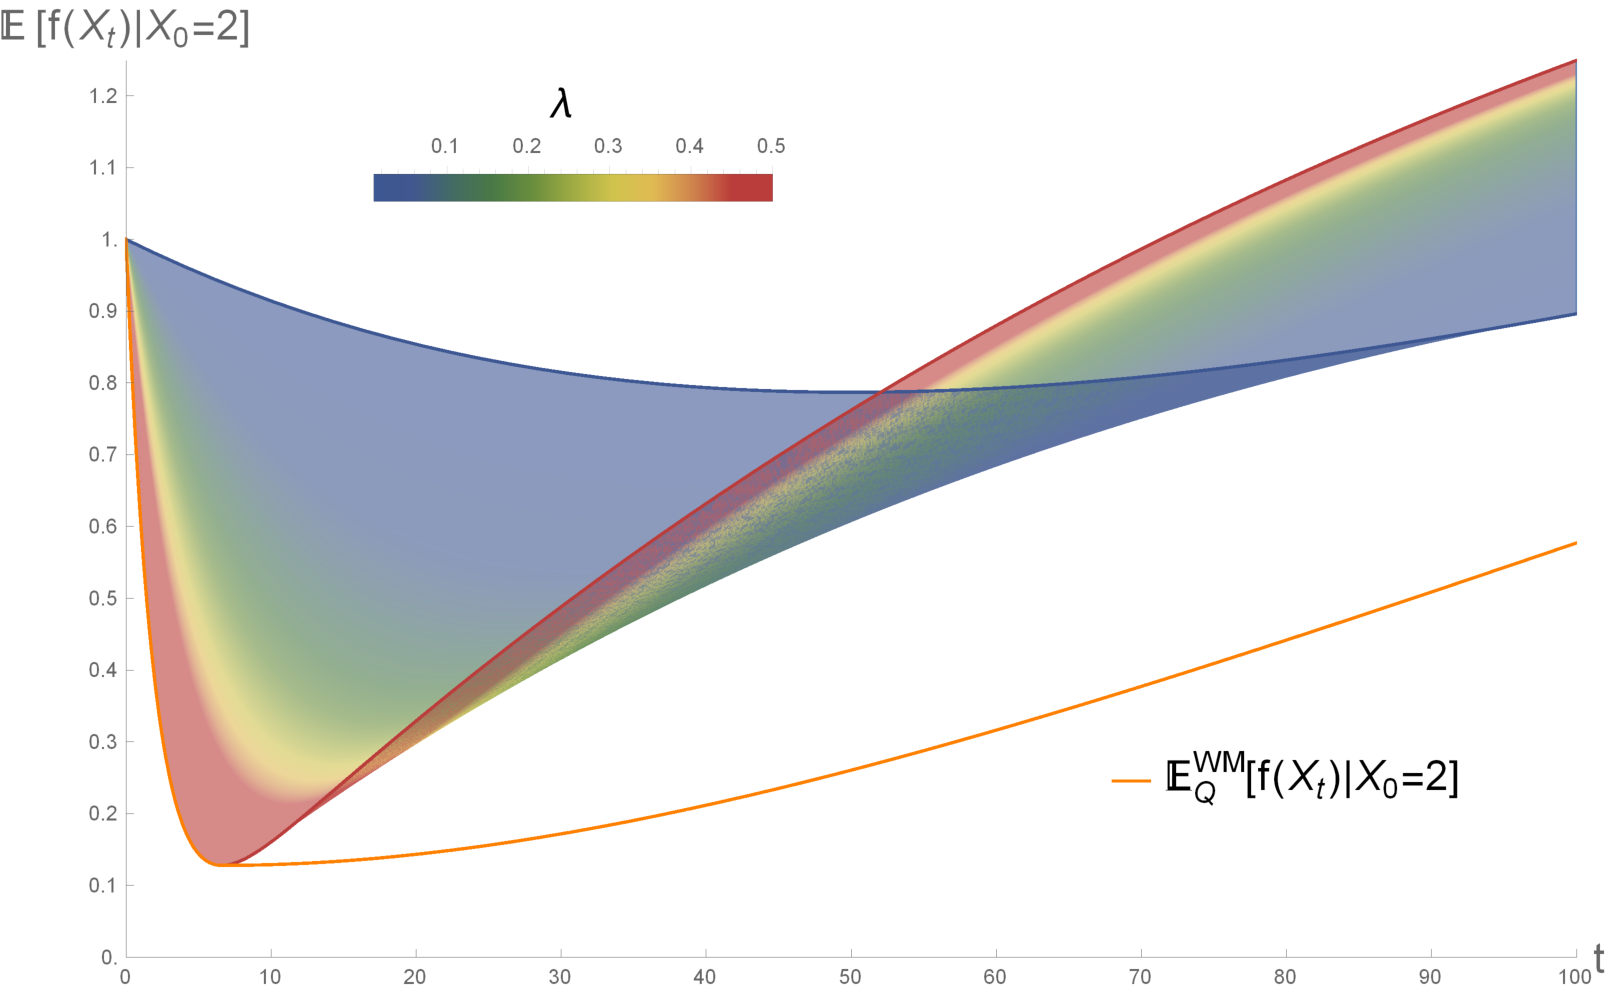
\includegraphics[width=106mm]{HomogeneousCounterExamplePicture}};
      \begin{scope}[x={(plot.south east)},y={(plot.north west)}]
        \draw[->] (0,0) -- (0,1.08) ;
        \node[left=0pt] at (0,1.04) {$q$};
        \draw[->] (0,0) -- (1.04,0) ;
        \node[below] at (1.06,0) {$t$}; 
        \draw (0,0) -- (0,-0.02);
        \node[below=3pt] at (0,0) {\small$0$};
        \draw (0.1,0) -- (0.1,-0.02);
        \node[below=3pt] at (0.1,0) {\small$10$};
        \draw (0.2,0) -- (0.2,-0.02);
        \node[below=3pt] at (0.2,0) {\small$20$};
        \draw (0.3,0) -- (0.3,-0.02);
        \node[below=3pt] at (0.3,0) {\small$30$};
        \draw (0.4,0) -- (0.4,-0.02);
        \node[below=3pt] at (0.4,0) {\small$40$}; 
        \draw (0.5,0) -- (0.5,-0.02);
        \node[below=3pt] at (0.5,0) {\small$50$}; 
        \draw (0.6,0) -- (0.6,-0.02);
        \node[below=3pt] at (0.6,0) {\small$60$}; 
        \draw (0.7,0) -- (0.7,-0.02);
        \node[below=3pt] at (0.7,0) {\small$70$}; 
        \draw (0.8,0) -- (0.8,-0.02);
        \node[below=3pt] at (0.8,0) {\small$80$}; 
        \draw (0.9,0) -- (0.9,-0.02);
        \node[below=3pt] at (0.9,0) {\small$90$}; 
        \draw (1,0) -- (1,-0.02);
        \node[below=3pt] at (1,0) {\small$100$}; 

        \draw (0,0) -- (-0.012,0);
        \node[left=3pt] at (0,0) {\small$0$};
        \draw (0,0.08) -- (-0.012,0.08);
        \node[left=3pt] at (0,0.08) {\small$0.1$};
        \draw (0,0.16) -- (-0.012,0.16);
        \node[left=3pt] at (0,0.16) {\small$0.2$};
        \draw (0,0.24) -- (-0.012,0.24);
        \node[left=3pt] at (0,0.24) {\small$0.3$};
        \draw (0,0.32) -- (-0.012,0.32);
        \node[left=3pt] at (0,0.32) {\small$0.4$};
        \draw (0,0.4) -- (-0.012,0.4);
        \node[left=3pt] at (0,0.4) {\small$0.5$};
        \draw (0,0.48) -- (-0.012,0.48);
        \node[left=3pt] at (0,0.48) {\small$0.6$};
        \draw (0,0.56) -- (-0.012,0.56);
        \node[left=3pt] at (0,0.56) {\small$0.7$};
        \draw (0,0.64) -- (-0.012,0.64);
        \node[left=3pt] at (0,0.64) {\small$0.8$};
        \draw (0,0.72) -- (-0.012,0.72);
        \node[left=3pt] at (0,0.72) {\small$0.9$};
        \draw (0,0.8) -- (-0.012,0.8);
        \node[left=3pt] at (0,0.8) {\small$1$};
        \draw (0,0.88) -- (-0.012,0.88);
        \node[left=3pt] at (0,0.88) {\small$1.1$};
        \draw (0,0.96) -- (-0.012,0.96);
        \node[left=3pt] at (0,0.96) {\small$1.2$};

		\node at (0.21,0.943) {$\lambda$};
        \draw (0.134,0.848) -- (0.134,0.86);
        \node at (0.134,0.887) {\scriptsize$0.1$};
        \draw (0.1812,0.848) -- (0.1812,0.86);
        \node at (0.1812,0.887) {\scriptsize$0.2$};
        \draw (0.2284,0.848) -- (0.2284,0.86);
        \node at (0.2284,0.887) {\scriptsize$0.3$};
        \draw (0.2756,0.848) -- (0.2756,0.86);
        \node at (0.2756,0.887) {\scriptsize$0.4$};
        \draw (0.3224,0.848) -- (0.3224,0.86);
        \node at (0.3224,0.887) {\scriptsize$0.5$};

        %\node at (0.06,0.88) {\footnotesize$0.01$};
        

        \node at (0.7,0.47) {$\underline{\mathbb{E}}_\rateset^\mathrm{WHM}[f(X_t)\,\vert\,X_0=a]$};
        \node at (0.82,0.23) {$\underline{\mathbb{E}}_\rateset^\mathrm{WM}[f(X_t)\,\vert\,X_0=a]$};
        \node at (0.87,0.15) {$~~~~=\underline{\mathbb{E}}_\rateset^\mathrm{W}[f(X_t)\,\vert\,X_0=a]$};
      \end{scope}
    \end{tikzpicture}
% 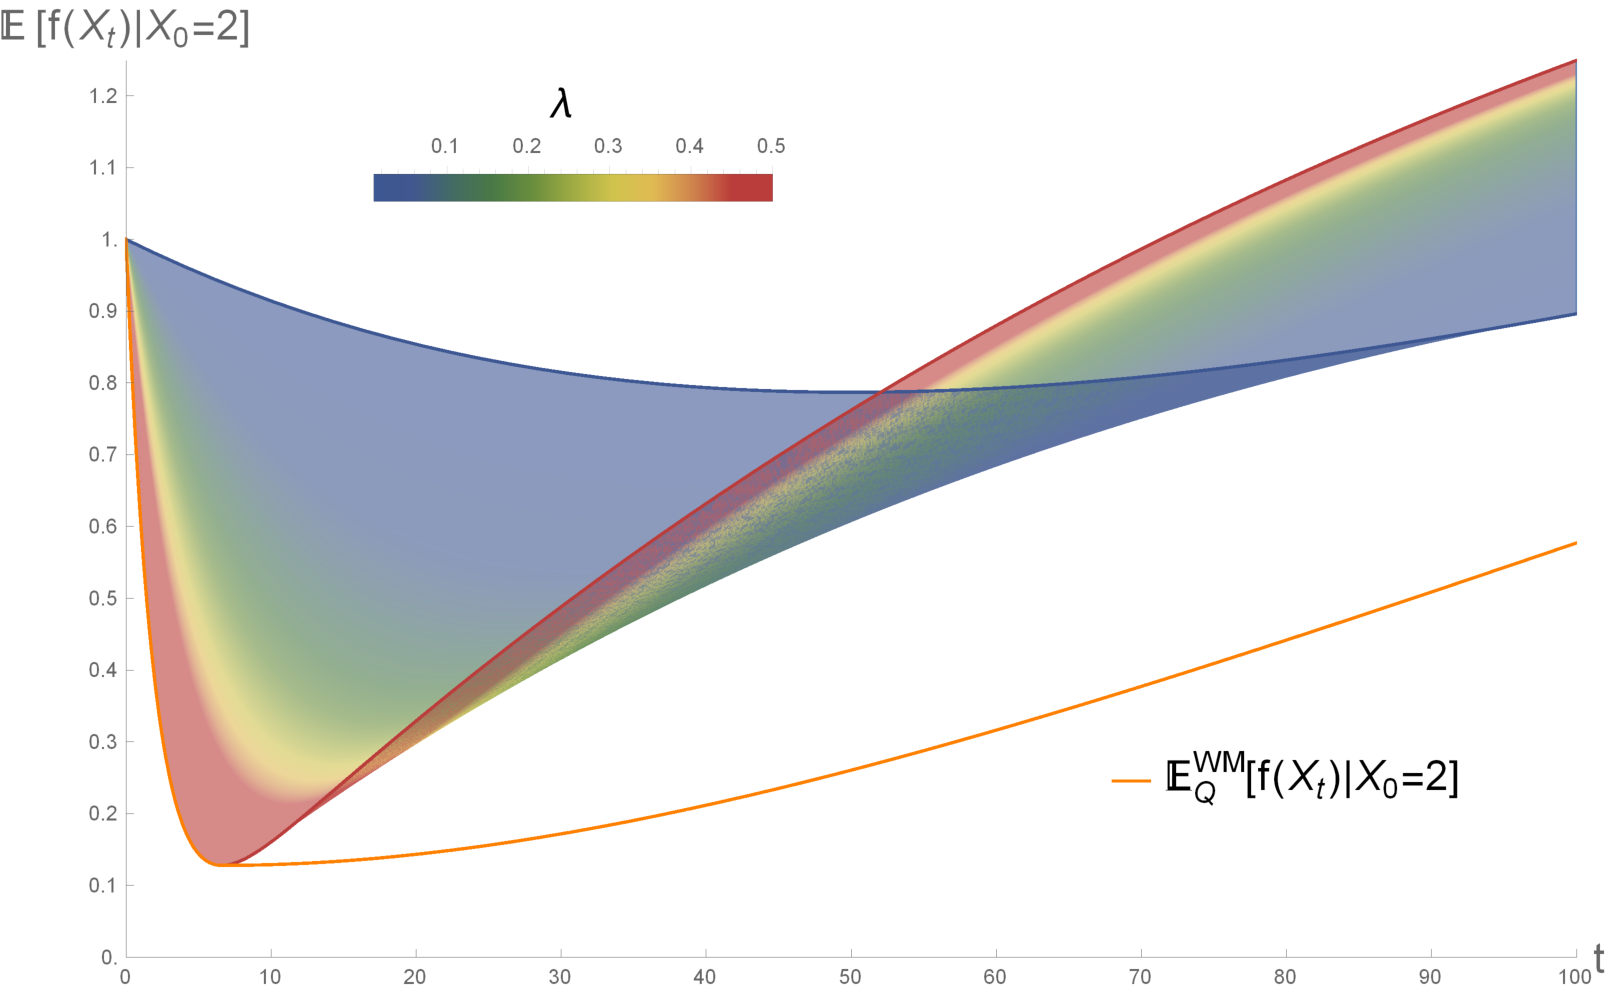
\includegraphics[width=\textwidth]{HomogeneousCounterExamplePicture}
\caption{Plot of the induced set of expected values $\mathbb{E}_P[f(X_t)\,\vert\,X_0=a]$, for time points $t\in[0,100]$, corresponding to all $P\in\whmprocesses_{\rateset}$ obtained as we vary $\lambda\in[0.01,0.5]$. Observe that the lower expectation with respect to this set is initially reached by choosing $\lambda=0.5$. This changes around the time-point $t\approx 6.6$, after which the minimizing value of $\lambda$ becomes a (changing) internal point of the interval $[0.01,0.5]$. The dashed line corresponds to the lower expectation with respect to the sets $\wmprocesses_\rateset$ and $\wprocesses_\rateset$, which also include non-homogeneous Markov chains and, for $\wprocesses_\rateset$, even more general processes. Note that the lower expectations with respect to $\whmprocesses_{\rateset}$, $\wmprocesses_{\rateset}$ and $\wprocesses_{\rateset}$ are all equal for $t<6.6$. However, as time evolves further, the lower expectation with respect to $\whmprocesses_{\rateset}$ starts to diverge from the other two.}
\label{fig:homogeneousCounterExample}
\end{figure}

\begin{exmp}\label{ex:homogeneousexample}
Consider an ordered ternary state space $\states\coloneqq \{a,b,c\}$,  let $f\in\gamblesX$ be defined as $f\coloneqq [1~0~2]^\top$---in the sense that $f(a)\coloneqq1$, $f(b)\coloneqq0$ and $f(c)\coloneqq2$---and consider the set of transition rate matrices
\vspace{4pt}
\begin{equation*}
\rateset \coloneqq \left\{ \left[\begin{array}{rrr}
-\lambda & \lambda & 0 \\
0 & -0.01 & 0.01 \\
0 & 0 & 0
\end{array}\right] \,:\,\lambda\in[0.01,0.5]\right\}.
\vspace{4pt}
\end{equation*}
Every process $P$ in the imprecise Markov chain $\whmprocesses_{\rateset,\,\mathcal{M}}$ is then a homogeneous Markov chain of which the unique transition rate matrix $Q$ is completely determined by some $\lambda$ in $[0.01,0.5]$. Furthermore, as we know from Remark~\ref{remark:expectationT} and Theorem~\ref{theo:homogeneoushasQ}, the conditional expectation $\mathbb{E}_P(f(X_t)\vert X_0=a)$ that corresponds to this homogeneous Markov chain is equal to $[e^{Q t}f](a)$. Due to this equality, it is a matter of applying some basic---yet cumbersome---algebra to find that 
\begin{align*}
\mathbb{E}_P[f(X_t)\vert X_0=a]
=
\begin{cases}
\displaystyle
2+e^{-\lambda t}+2\frac{e^{-\lambda t}-100\lambda e^{-\nicefrac{t}{100}}}{100\lambda-1}&\text{ if $\lambda\in(0.01,0.5]$}\\[8pt]
\displaystyle
2-e^{-\nicefrac{t}{100}}-\frac{1}{50}te^{-\nicefrac{t}{100}}&\text{ if $\lambda=0.01$.}
\end{cases}
\end{align*}
Obtaining the value of $\underline{\mathbb{E}}_{\rateset,\,\mathcal{M}}^{\mathrm{WHM}}[f(X_t)\,\vert\,X_0=a]$ now corresponds to minimising this expression as $\lambda$ ranges over the interval $[0.01,0.5]$. Figure~\ref{fig:homogeneousCounterExample} illustrates that, even in this simple ternary case, this minimisation problem is already non-trivial, because---depending on the value of $t$---the minimum is not guaranteed to obtained for one of the end points of $[0.01,0.5]$, but may only be achieved by an internal point. Nevertheless, in this simple case, $\underline{\mathbb{E}}_{\rateset,\,\mathcal{M}}^{\mathrm{WHM}}[f(X_t)\,\vert\,X_0=a]$ can of course be computed by brute force, leading to the solution that is depicted in Figure~\ref{fig:homogeneousCounterExample}. 

Figure~\ref{fig:homogeneousCounterExample} also depicts $\underline{\mathbb{E}}_{\rateset,\,\mathcal{M}}^{\mathrm{WM}}[f(X_t)\,\vert\,X_0=a]$ and $\underline{\mathbb{E}}_{\rateset,\,\mathcal{M}}^{\mathrm{W}}[f(X_t)\,\vert\,X_0=a]$, which happen to coincide. The reason why they coincide in this case, and the method by which we have computed them, will be explained in Section~\ref{sec:connections}. For now, it suffices to notice that for large enough values of $t$, their common value differs from $\underline{\mathbb{E}}_{\rateset,\,\mathcal{M}}^{\mathrm{WHM}}[f(X_t)\,\vert\,X_0=a]$, thereby illustrating that the first inequality in Proposition~\ref{prop:lower_exp_markov_bounded_by_nonmarkov} can indeed be strict.
% \begin{align*}
% \underline{\mathbb{E}}_{\rateset,\,\mathcal{M}}^{\mathrm{WHM}}[f(X_t)\,\vert\,X_0=]
% &=
% \inf\left\{ [e^{Q t}f](x_0)\,:\,Q\in\rateset\right\}\\
% &=
% \begin{cases}
% test
% \end{cases}
% \end{align*}
%The below picture should work for this example (y-axis is still labeled incorrectly though by a factor of 50). X-axis is time, y-axis is expected value conditional on $X_0=2$, the colored area is the set of $\{\mathbb{E}_P[f(X_t)\,\vert\,X_0=2]\,:\,P\in\whmprocesses_\rateset\}$, obtained by varying $\lambda\in[0.01,0.5]$, and the orange line is lower expectation for non-Markov \ictmc, $\underline{\mathbb{E}}_\rateset^\mathrm{WM}[f(X_t)\,\vert\,X_0=2]$. I feel this is a clear illustration that the lower expectations are different :)
%*** Mathematica actually breaks down when I try to use the build-in solver for this. Interestingly, it works perfectly fine for time points less than 6.6, which is around the point where the "desired-state" switch occurs and homogeneity breaks down. Anyway, I used a $1000\times 1000$-grid discretization of the above $\rateset$, then just optimized over that to find the answer.
%By comparison, for the non-homogeneous case, the optimization using Algorithm~\ref{alg:compute_singlevar}, with $\epsilon=10^{-3}$, gives
%\begin{equation*}
%\underline{\mathbb{E}}_{\rateset}^\mathrm{WM}[f(X_{10})\,\vert\,X_0=2] \approx 0.129\pm 10^{-3}\,,
%\end{equation*}
%which should establish the difference within error tolerances.
\exampleend
\end{exmp}

While numerically solving the type of non-linear optimization problems that are associated with $\underline{\mathbb{E}}^\mathrm{WHM}_{\rateset\,,\mathcal{M}}$ is feasible for sufficiently ``nice'' sets $\rateset$ in low dimensions---as was the case in our example---the computational complexity will in general quickly explode as the size of $\states$ increases.
Therefore, computing lower expectations for \ictmc's that are of the type $\smash{\whmprocesses_{\rateset,\,\mathcal{M}}}$ is typically intractable, and it is then necessary to resort to approximation methods. For the particular case where $\rateset$ corresponds to an interval matrix, such methods have been explored in, for example, References \cite{Goldsztejn2014} and~\cite{oppenheimer1988}. 

%In contrast, for lower expectations of the type $\smash{\underline{\mathbb{E}}_{\rateset,\,\mathcal{M}}^{\mathrm{WM}}}$ or $\smash{\underline{\mathbb{E}}_{\rateset,\,\mathcal{M}}^{\mathrm{W}}}$ as we will show later in this work, efficient computations are definitely possible.
%\exampleend
%\end{exmp}
%In fact, even for the particular case where $\rateset$ corresponds to an interval matrix, the problem is already NP-hard~\cite{Goldsztejn2014}.


In the remainder of this paper, we do not consider \ictmc's that are of the type $\smash{\whmprocesses_{\rateset,\,\mathcal{M}}}$. Instead, we will focus on the lower expectations $\smash{\underline{\mathbb{E}}_{\rateset,\mathcal{M}}^\mathrm{WM}}$ and $\smash{\underline{\mathbb{E}}_{\rateset,\mathcal{M}}^\mathrm{W}}$ that correspond to \ictmc's that are of the type $\smash{\wmprocesses_{\rateset,\,\mathcal{M}}}$ or $\smash{\wprocesses_{\rateset,\,\mathcal{M}}}$, and we will develop efficient methods for computing them. In order to do that, we start by introducing the notion of a lower transition operator.


%, having introduced \ictmc's of the type $\smash{\whmprocesses_{\rateset,\,\mathcal{M}}}$ only for the sake of completeness. %Of course, because of Proposition~\ref{prop:lower_exp_markov_bounded_by_nonmarkov}, $\smash{\underline{\mathbb{E}}_{\rateset,\mathcal{M}}^\mathrm{WM}}$ and $\smash{\underline{\mathbb{E}}_{\rateset,\mathcal{M}}^\mathrm{W}}$ both provide a lower bound for $\underline{\mathbb{E}}_{\rateset,\,\mathcal{M}}^\mathrm{WHM}$. However, this bounds will in general not be tight if one insists that the analysis should be done with respect to $\whmprocesses_{\rateset,\,\mathcal{M}}$. %However, since this latter \ictmc~does make the strictest---and, we would argue, most unrealistic---assumptions about the domain of interest, we do not consider this particularly problematic.





\section{Towards Lower Transition Operators for \ictmc's}
\label{sec:lowertrans}

%Having introduced lower expectations that correspond to sets of processes that may not be homogeneous and that may not even satisfy the Markov property, one might wonder how to compute these lower expectations, either numerically or for analytical purposes. Indeed, one of the aims of this paper is to provide methods with which such lower expectations can be tractably computed.

%Obviously, one way to compute a lower expectation is to work directly with the definition. That is, explicitly generate the entire set $\wmprocesses_{\rateset,\,\mathcal{M}}$ (or $\wprocesses_{\rateset,\,\mathcal{M}}$) for a given $\rateset$ and $\mathcal{M}$, compute expectations of a function $f$ for each element of this set, and then find the infimum of these expectations. It should be clear that this approach is fairly unwieldy, not in the least because for arbitrary $\rateset$ the corresponding set of processes may be infinite. Therefore, we will instead provide an alternative characterization of this lower expectation.

As explained in Remark~\ref{remark:expectationT}, the transition matrix $T_t^s$ of a stochastic process $P$ serves as an alternative representation of the expectation operator $\mathbb{E}_P[f(X_s)\,\vert\,X_t]$, in the sense that
\begin{equation}\label{eq:transitionmatrixasexpectation}
[T_t^sf](x_t)=\mathbb{E}_P[f(X_s)\,\vert\,X_t=x_t]
\text{ for all $f\in\gamblesX$ and $x_t\in\states$.}
\end{equation}
Furthermore, if $P$ is a well-behaved homogeneous Markov chain, then as explained in Section~\ref{sec:homogen_markov_chain}, $T_t^s$ is completely determined by a unique transition rate matrix $Q$, in the sense that $T_t^s=e^{Q(s-t)}$.

We will in this section introduce a generalization of these transition matrices and transition rate matrices, called \emph{lower transition operators} and \emph{lower transition rate operators}, respectively. Furthermore, and most importantly, we will introduce the notion of a \emph{corresponding lower transition operator}, which, much like in the precise homogeneous case, will be completely determined by some given lower transition rate operator. 

Further on in this paper, we will then  show that this type of lower transition operator serves as an alternative representation for the lower expectations of imprecise continuous-time Markov chains, thereby establishing an analogy with Equation~\eqref{eq:transitionmatrixasexpectation}. However, for now, in this section, we focus on introducing the relevant concepts, and on deriving this operator of interest. We end in Section~\ref{sec:properties_lower_trans} by showing that this operator satisfies a number of convenient properties.
%We will in this section introduce a \emph{lower transition operator}, which is a map from $\gamblesX$ to $\gamblesX$ that generalizes the notion of a transition matrix. We will here focus on introducing the relevant concepts, and showing that this operator of interest is well-defined. We end this section by establishing that this (family) of operators is in many ways intuitively comparable to the transition matrix system of a well-behaved homogeneous Markov chain. In Section~\ref{sec:connections} we will then establish the relation between this operator and lower expectations, and show that we can indeed use it to compute the quantities of interest. In Section~\ref{sec:prev_work} we will show how this operator is related to previous work from the literature.

\subsection{Lower Transition Operators}\label{subsec:lowertrans_rate}

The central concept that we will be interested in throughout this section is that of a lower transition operator $\lt$.

\begin{definition}[Lower Transition Operator]\label{def:coh_low_trans}
A map $\lt$ from $\gamblesX$ to $\gamblesX$ is called a \emph{lower transition operator} if, for all $f,g\in\gamblesX$, all $\lambda\in\realsnonneg$, and all $x\in\states$:
%\vspace{5pt}
\begin{enumerate}[label=LT\arabic*:,ref=LT\arabic*]
\item
$\left[\lt\,f\right](x)\geq\min\left\{f(y)\,\colon\,y\in\states\right\}$ \label{LT:bounded_min}
\item
$\left[\lt(f+g)\right](x)\geq \left[\lt\,f\right](x)+\left[\lt\,g\right](x)$; \label{LT:super_additive}
\item
$\left[\lt(\lambda f)\right](x)=\lambda\left[\lt\,f\right](x)$. \label{LT:homo}
\end{enumerate}
%\vspace{5pt}
\noindent We will use $\underline{\mathbb{T}}$ to denote the set of all lower transition operators.

Such lower transition operators furthermore satisfy the following properties---see Reference~\cite{DeBock:2016} for a proof. For any lower transition operator $\lt$, any $f_1,f_2\in\gamblesX$ and any two non-negatively homogeneous operators $A,B$ from $\gamblesX$ to $\gamblesX$:
\begin{enumerate}[label=LT\arabic*:,ref=LT\arabic*,start=4]
\item
$\norm{\lt} \leq 1$; \label{LT:norm_at_most_one}
\item
$f_1\geq f_2~\then~\lt f_1\geq\lt f_2$;\label{LT:monotonicity}
\item
$\norm{\lt A - \lt B} \leq \norm{A - B}$. \label{LT:differencenorm}
\end{enumerate}
\vspace{0pt}
\end{definition}

\begin{proposition}\label{lemma:compositioncoherence}
For any two lower transition operators $\lt,\underline{S}\in\underline{\mathbb{T}}$, their composition $\lt\,\underline{S}$ is again a lower transition operator.% $\left(\lt\,\underline{S}\right)\in\underline{\mathbb{T}}$.
\end{proposition}

The first thing to note is that any transition matrix $T$ will also satisfy properties~\ref{LT:bounded_min}-\ref{LT:homo}, and hence is also a lower transition operator. It is therefore clear that lower transition operators are a generalization of transition matrices.

A first way to motivate this specific generalization is to note the following. For any lower transition operator $\lt$ and any $x\in\states$, consider the map $\lt_x:\gamblesX\to\reals$, defined for all $f\in\gamblesX$ as
\begin{equation}\label{eq:lowerprevisionfromlt}
\lt_xf \coloneqq \left[\lt f\right](x)\,.
\end{equation}
Due to properties~\ref{LT:bounded_min}-\ref{LT:homo}, it then follows that $\lt_x$ is a map from $\gamblesX$ to $\reals$ that is super-additive, non-negatively homogeneous, and bounded below by the minimum operator. By definition~\cite[Definition~2.3.3]{Walley:1991vk}, that means that $\lt_x$ is a \emph{coherent lower prevision} on $\gamblesX$. Note that the term ``prevision'' here is a synonym for ``expectation''---be it with a different interpretation attached to it---so this essentially states that $\lt_x$ is a ``coherent lower expectation'' on $\gamblesX$.

For the reader that is unfamiliar with this notion of coherent lower previsions, this is perhaps best clarified as follows. Consider some arbitrary set $\mathcal{M}$ of probability mass functions on $\states$, and consider a map $\underline{\mathbb{E}}:\gamblesX\to\reals$, defined for all $f\in\gamblesX$ as
\begin{equation*}
\underline{\mathbb{E}}f \coloneqq \inf\left\{\sum_{x\in\states} p(x)f(x)\,:\,p\in\mathcal{M}\right\}\,.
\end{equation*}
We call this map $\underline{\mathbb{E}}$ the \emph{lower envelope} of $\mathcal{M}$, and it should be clear that this map computes a lower expectation with respect to $\mathcal{M}$. Furthermore, note that for any $p\in\mathcal{M}$, the quantity $\sum_{x\in\states}p(x)f(x)$ is bounded from below by $\min\{f(y):y\in\states\}$, and since this is true for any $p\in\mathcal{M}$, it follows that $\underline{\mathbb{E}}f$ is also bounded below by this minimum. Similarly, it is easily verified that $\underline{\mathbb{E}}$ is super-additive and non-negatively homogeneous, due to the properties of the $\inf$ operator. Hence, by the definition cited above, the lower expectation operator $\underline{\mathbb{E}}$ that corresponds to $\mathcal{M}$ is a coherent lower prevision on $\gamblesX$. 

Our consideration of the coherent lower prevision $\lt_x$  above is essentially the same idea, but \emph{without} considering explicitly any link to some set of probability mass functions $\mathcal{M}_x$. Suffice it to say that, for any coherent lower prevision $\lt_x$, such a set $\mathcal{M}_x$ will always exist~\cite[Section 10.2]{Huber:1981ch}. It should furthermore be noted that the qualifier ``coherent'' here has connections to the notion of coherence that appeared in Section~\ref{sec:cond_prob}, and that it can be given a direct gambling interpretation that resembles the one in Appendix~\ref{app:coherence}; we refer to~\cite{troffaes2013:lp,Walley:1991vk} for further discussion on this.

In any case, for our present purposes, it suffices to realise that, because $\lt_x$ is a coherent lower prevision for any $x\in\states$, the lower transition operator $\lt$ can be seen as a vector of coherent lower previsions. Therefore, and because each of these coherent lower previsions $\lt_x$ has some set $\mathcal{M}_x$ of probability mass functions of which $\lt_x$ computes the lower envelope, we can combine these sets of probability mass functions to form a set of transition matrices
\begin{equation*}
\mathfrak{T}=\{T\in\mathbb{T}\colon (\forall x\in\states)~T(x,\cdot)\in\mathcal{M}_x\}
\end{equation*}
of which $\lt$ is the lower envelope, in the sense that
\begin{equation*}
[\lt f](x) = \inf\{ [Tf](x)\,:\, T\in\mathfrak{T} \}~
\text{ for all $f\in\gamblesX$ and $x\in\states$.}
\end{equation*}
Due to the correspondence between transition matrices and conditional expectation operators---see Remark~\ref{remark:expectationT}---it should therefore be clear that lower transition operators are an intuitive starting point to try and find alternative characterizations for the lower expectations that correspond to an \ictmc. What remains is to find the specific lower transition operator $\lt$ whose set of dominating transition matrices $\mathfrak{T}$ corresponds to the set of transition matrices that is induced by a given \ictmc; the remainder of this section will provide the machinery required to do this.

%\begin{proposition}\label{lem:normlratefinite}
%For any lower transition rate operator $\lrate$, we have that $0\leq\norm{\lrate}<+\infty$.
%\end{proposition}
%
%\begin{proposition}\label{lemma:normofcoherenttrans}
%For any lower transition operator $\lt$, we have that $0\leq \norm{\lt}\leq 1$.
%\end{proposition}

We conclude with the following result about the set $\underline{\mathbb{T}}$ of all lower transition operators, which states that this set is a complete metric space with respect to our usual norm.

\begin{proposition}\label{lemma:completemetricspace}
The metric space $(\underline{\mathbb{T}},d)$ is complete with respect to the metric $d$ that is induced by our usual norm $\norm{\cdot}$.
\end{proposition}

\subsection{Lower Transition Rate Operators}\label{sec:connections_rate}

We next focus on the generalization of transition rate matrices $Q$ to lower transition rate operators $\lrate$, as follows.
\begin{definition}[Lower Transition Rate Operator]\label{def:coh_low_trans_rate}
A map $\lrate$ from $\gamblesX$ to $\gamblesX$ is called a \emph{lower transition rate operator} if, for all $f,g\in\gamblesX$, all $\lambda\in\realsnonneg$, all constant functions $\mu\in\gamblesX$, and all $x\in\states$:

%\vspace{5pt}
\begin{enumerate}[label=LR\arabic*:,ref=LR\arabic*]
\item\label{LR:constantzero}
$\left[\lrate\mu\right](x)=0$;
\item\label{LR:nondiagpos}
$\left[\lrate\ind{y}\right](x)\geq0$ for all $y\in\states$ such that $x\neq y$;
\item\label{LR:subadditive}
$\left[\lrate(f+g)\right](x)\geq\left[\lrate f\right](x)+\left[\lrate g\right](x)$;
\item\label{LR:homo}
$\left[\lrate(\lambda f)\right](x)= \lambda\left[\lrate f\right](x)$.
\end{enumerate}
%\vspace{5pt}
Such lower transition rate operators furthermore satisfy the following properties---see Reference~\cite{DeBock:2016} for a proof. For any lower transition rate operator $\lrate$ and any two non-negatively homogeneous operators $A,B$ from $\gamblesX$ to $\gamblesX$:
\begin{enumerate}[label=LR\arabic*:,ref=LR\arabic*,start=5]
\item
$\norm{\lrate} < +\infty$ \label{LR:normlratefinite};
\item
$\norm{\lrate A - \lrate B} \leq 2\norm{\lrate}\norm{A - B}.$ \label{LR:differenceofnorm}
\end{enumerate}
\vspace{0pt}
\end{definition}

Note that properties~\ref{LR:constantzero} and~\ref{LR:nondiagpos} essentially preserve properties~\ref{def:Q:sumzero} and~\ref{def:Q:nonnegoffdiagonal} from Definition~\ref{def:rate_matrix}. The main difference lies in the fact that a rate matrix $Q$ is a linear map, whereas properties~\ref{LR:subadditive} and~\ref{LR:homo} merely require that a lower transition rate operator $\lrate$ is super-additive and non-negatively homogeneous. Therefore, every rate matrix is clearly a lower transition rate operator, with the latter concept providing a generalization of the former.

A first reason why this specific generalization is of interest, is because it preserves the relation between transition matrices and rate matrices that was established in Propositions~\ref{prop:stochastic_from_rate_matrix} and~\ref{prop:rate_from_stochastic_matrix}. Indeed, the following two results generalise these relations to our current setting.

%**** We next establish that there is a correspondence between lower transition rate operators and lower transition operators that is analogous to the one found in Section~\ref{sec:trans_rate_matrices}.

\begin{proposition}[Reference {\cite[Proposition 5]{DeBock:2016}}]\label{lemma:normQsmallenough}
Consider any lower transition rate operator $\lrate$, and any $\Delta\in\realsnonneg$ such that $\Delta\norm{\lrate}\leq 1$. Then the operator $(I+\Delta\lrate)$ is a lower transition operator.
\end{proposition}

\begin{proposition}[Reference {\cite[Proposition 6]{DeBock:2016}}]\label{lemma:lower_trans_to_lower_rate}
Consider any lower transition operator $\lt$, and any $\Delta\in\realspos$. Then the operator $\nicefrac{1}{\Delta}(\lt - I)$ is a lower transition rate operator.
\end{proposition}

Now, in our discussion of lower transition operators in Section~\ref{subsec:lowertrans_rate}, we mentioned that lower transition operators can be interpreted as the lower envelope of a set of transition matrices. As we are about to show, there is a similar connection between lower transition rate operators and sets of rate matrices.

So consider any non-empty bounded set $\rateset\subseteq\mathcal{R}$ of rate matrices. Then for any $f\in\gamblesX$, if we let
\begin{equation}\label{eq:correspondinglowertrans}
[\lrate f](x)\coloneqq\inf\{[Qf](x)\colon Q\in\rateset\}
\text{ for all $x\in\states$},%\\[2mm],
\end{equation}
the resulting function $\lrate f$ is again an element of $\gamblesX$,\footnote{%Since $\rateset$ is non-empty, the components of $\lrate f$ cannot be $+\infty$.
Since $\rateset$ is bounded,~\ref{N:normAf} implies that, for all $Q\in\rateset$, $\norm{Qf}\leq\norm{Q}\norm{f}\leq\norm{\rateset}\norm{f}<+\infty$. Therefore, and since $\rateset$ is non-empty, the components of $\lrate f$ are bounded below by $-\norm{\rateset}\norm{f}$, which implies that $\lrate f$ is a real-valued function on $\states$.}
and therefore, $\lrate$ is a map from $\gamblesX$ to $\gamblesX$. We call this operator $\lrate$, as defined by Equation~\eqref{eq:correspondinglowertrans}, the \emph{lower envelope} of $\rateset$. It is a matter of straightforward verification to see that $\lrate$ is a lower transition rate operator.

\begin{proposition}\label{prop:lowerenvelopeislowertrans}
For any non-empty bounded set $\rateset\subseteq\mathcal{R}$ of rate matrices, the corresponding operator $\lrate\colon\gamblesX\to\gamblesX$, as defined by Equation~\eqref{eq:correspondinglowertrans}, is a lower transition rate operator.
\end{proposition}

\noindent
Inspired by this result, we will also refer to the lower envelope of $\rateset$ as the \emph{lower transition rate operator that corresponds to $\rateset$}. %As we have just seen, every non-empty bounded set $\rateset\subseteq\mathcal{R}$ of rate matrices has such a corresponding lower transition rate operator $\lrate$. 
However, this correspondence is not one-to-one. As the following example establishes, different non-empty bounded sets of rate matrices may have the same corresponding lower transition rate operator.

\begin{exmp}\label{example:different_sets_same_lower_rate}
For the sake of simplicity, we assume that the state space $\states$ has only two elements, which allows us to work with $2\times 2$ matrices. Consider now two rate matrices
\begin{equation*}
A\coloneqq\left[\begin{array}{rr}-1 & 1 \\2 & -2\end{array}\right]\quad\text{and}\quad
B\coloneqq\left[\begin{array}{rr}-3 & 3 \\1 & -1\end{array}\right]\,,
\vspace{7pt}
\end{equation*}
let $C\coloneqq \nicefrac{1}{2}(A+B)$ be their convex mixture, which is clearly also a rate matrix, and use these matrices to define the sets $\rateset_1\coloneqq\{A,B\}$ and $\rateset_2\coloneqq\{A,B,C\}$. Then clearly, $\rateset_1$ and $\rateset_2$ are two different, non-empty and bounded sets of rate matrices. Nevertheless, as we are about to show, the corresponding lower transition rate operators are identical.

Let $\lrate_1$ and $\lrate_2$ be the lower transition rate operators that correspond to $\rateset_1$ and $\rateset_2$, respectively, %We will show that $\lrate_1=\lrate_2$.
and consider any $f\in\gamblesX$. Equation~\eqref{eq:correspondinglowertrans} then implies that $\lrate_1f\leq Af$ and $\lrate_1f\leq Bf$, which in turn implies that $\lrate_1f\leq Cf$. Therefore, by applying Equation~\eqref{eq:correspondinglowertrans} once more, we find that $\lrate_1 f\leq\lrate_2 f$. Hence, since Equation~\eqref{eq:correspondinglowertrans} also trivially implies that $\lrate_2 f\leq\lrate_1 f$, we find that $\lrate_1 f=\lrate_2 f$. Since this is true for any $f\in\gamblesX$, we conclude that $\lrate_1=\lrate_2$.
\exampleend
\end{exmp}
Of course, this should not really be surprising---Example~\ref{example:different_sets_same_lower_rate} essentially establishes that different sets can have the same infimum. However, it does lead to a natural question: what do these different sets have in common?

Therefore, we next consider some fixed lower transition rate operator $\lrate$.
All the non-empty bounded sets $\rateset$ of rate matrices that have $\lrate$ as their lower envelope then share a common property: they consist of rate matrices $Q$ that dominate $\lrate$, in the sense that $Qf\geq\lrate f$ for all $f\in\gamblesX$. Therefore, each of these sets $\rateset$ is contained in the following set of dominating rate matrices:
\begin{equation}\label{eq:dominatingratematrices}
\rateset_{\lrate}\coloneqq
\left\{
Q\in\mathcal{R}
\colon
Qf\geq\lrate f\text{ for all $f\in\gamblesX$}
\right\}.
\end{equation}
As our next result shows, this set $\rateset_{\lrate}$ is non-empty and bounded, and has $\lrate$ as its lower envelope. Even stronger, the infimum in Equation~\eqref{eq:correspondinglowertrans} is reached---can be replaced by a minimum.

\begin{proposition}\label{prop:dominating_nonempty_bounded}
Consider a lower transition rate operator $\lrate$ and let $\rateset_{\lrate}$ be the corresponding set of dominating rate matrices, as defined by Equation~\eqref{eq:dominatingratematrices}. Then $\rateset_{\lrate}$ is non-empty and bounded and, for all $f\in\gamblesX$, there is some $Q\in\rateset_{\lrate}$ such that $\lrate f=Qf$.
\end{proposition}

\noindent
Because of this result, and since---as discussed above---every non-empty bounded set of rate matrices that has $\lrate$ as its lower envelope is a subset of $\rateset_{\lrate}$, it follows that $\rateset_{\lrate}$ is the largest non-empty bounded set of rate matrices that has $\lrate$ as its lower envelope.
Furthermore, as we show in Proposition~\ref{prop:dominatingproperties} below, this set $\rateset_{\lrate}$ is also closed and convex, and has what we call \emph{separately specified rows}. 

Intuitively, we say that a set $\rateset$ of rate matrices has separately specified rows if it is closed under taking arbitrary combinations of rows from its elements. More formally, if for every $x\in\states$ we let $\rateset_x\coloneqq\{Q(x,\cdot):Q\in\rateset\}$ denote the set of $x$-rows of the matrices in $\rateset$, then we say that $\rateset$ has separately specified rows if $\rateset$ contains every matrix $Q$ that can be constructed by selecting, for all $x\in\states$, an arbitrary row $Q(x,\cdot)$ from $\rateset_x$.

\begin{definition}\label{def:separatelyspecifiedrows}
A set of rate matrices $\rateset\subseteq\mathcal{R}$ has separately specified rows if
\begin{equation*}
\rateset=\left\{
Q\in\mathcal{R}
\colon
(\forall x\in\states)~Q(x,\cdot)\in\rateset_x\right\},
\end{equation*}
where, for every $x\in\states$, $\rateset_x\coloneqq\{Q(x,\cdot)\colon Q\in\rateset\}$ is some given set of rows from which the $x$-row $Q(x,\cdot)$ of the rate matrices $Q$ in $\rateset$ is selected, independently of the other rows.
\end{definition}

\begin{proposition}\label{prop:dominatingproperties}
Consider a lower transition rate operator $\lrate$ and let $\rateset_{\lrate}$ be the corresponding set of dominating rate matrices, as defined by Equation~\eqref{eq:dominatingratematrices}. Then $\rateset_{\lrate}$ is closed and convex, and has separately specified rows.
\end{proposition}

\noindent
These additional properties characterize $\rateset_{\lrate}$ completely, in the sense that no other set satisfies them.

\begin{proposition}\label{prop:dominating_unique_characterization}
Consider any non-empty, bounded, closed and convex set of rate matrices $\rateset\subseteq\mathcal{R}$ with separately specified rows that has $\lrate$ as its lower envelope. Then $\rateset=\rateset_{\lrate}$.
\end{proposition}

\begin{exmp}\label{ex:dominatingset}
Let $\rateset_1$ and $\rateset_2$ be constructed as in Example~\ref{example:different_sets_same_lower_rate}, and let $\lrate\coloneqq\lrate_1=\lrate_2$ be their common lower transition rate operator. As we are about to show, the corresponding set of dominating rate matrices $\rateset_{\lrate}$ is then equal to
\begin{equation}\label{eq:ex:dominatingset:globaldef}
\rateset^* \coloneqq \{Q\in\mathcal{R}\,:\,(\forall x\in\states)\, Q(x,\cdot)\in\rateset_x\},
\end{equation}
where, for all $x\in\states$, $\rateset_x$ is given by
\begin{equation}\label{eq:ex:dominatingset:localdef}
\rateset_x \coloneqq \left\{\lambda A(x,\cdot)+(1-\lambda)B(x,\cdot)\,:\,\lambda\in[0,1]\right\}.
\end{equation}

First of all, for any $Q\in\rateset^*$, $f\in\gamblesX$ and $x\in\states$, it follows from Equations~\eqref{eq:ex:dominatingset:globaldef} and~\eqref{eq:ex:dominatingset:localdef} that there is some $\lambda\in[0,1]$ such that
\begin{equation*}
[Qf](x)=\lambda[Af](x)+(1-\lambda)[Bf](x)
\geq\lambda[\lrate f](x)+(1-\lambda)[\lrate f](x)
=[\lrate f](x),
\end{equation*}
where the inequality holds because $\lrate$ is the lower envelope of $\rateset_1$. Since this is true for all $x\in\states$, we find that $Qf\geq\lrate f$. Since this is true for all $f\in\gamblesX$ and all $Q\in\rateset^*$, it follows that $\rateset^*\subseteq\rateset_{\lrate}$. 


Let now $\lrate^*$ be the lower transition rate operator that corresponds to $\rateset^*$ and consider any $f\in\gamblesX$. Then, because $\rateset^*\subseteq\rateset_{\lrate}$, we find that $\lrate^*f\geq\lrate f$. Similarly, since $\rateset_1$ is clearly a subset of $\rateset^*$, we find that $\lrate^*f\leq\lrate_1f$. Since $\lrate_1=\lrate$, it follows that $\lrate f\leq \lrate^*f\leq \lrate f$, and because this holds for any $f\in\gamblesX$, we conclude that $\lrate^*=\lrate$.


% Recall from Example~\ref{example:different_sets_same_lower_rate} that for all $f\in\gamblesX$, it holds that either $\lrate f=Af$, or $\lrate f=Bf$. Using a similar argument as we used there for the rate matrix $C$, it is clear that any convex combination $Q_\lambda\coloneqq \lambda A+(1-\lambda)B$, with $\lambda\in[0,1]$, is a rate matrix that dominates $\lrate$. Furthermore, because we there found that $[Af](1)\leq [Bf](1)$ if and only if $[Af](2)\leq[Bf](2)$, any matrix constructed by combining rows from $A$ and $B$ will dominate $\lrate$. For example, let $D$ be a rate matrix such that $D(1,\cdot)\coloneqq A(1,\cdot)$ and $D(2,\cdot)\coloneqq B(2,\cdot)$. Then, if $Af\leq Bf$, it also holds that $Af\leq Df$. Similarly, if $Bf\leq Af$, then also $Bf\leq Df$. A similar argument shows that the same is true for any matrix constructed by combining rows from different convex combinations of $A$ and $B$.

% From these ideas, we first construct two sets of rows. For all $x\in\states$, let
% \begin{equation*}
% \rateset_x \coloneqq \left\{\lambda A(x,\cdot)+(1-\lambda)B(x,\cdot)\,:\,\lambda\in[0,1]\right\}\,.
% \end{equation*}
% Let now $\rateset \coloneqq \{Q\in\mathcal{R}\,:\,(\forall x\in\states)\, Q(x,\cdot)\in\rateset_x\}$. Then, for all $Q\in\rateset$, $Q$ is such that
% \begin{equation*}
% Q=\left[\begin{array}{rr}-a & a \\ b& -b\end{array}\right]\,,\quad\text{where $a\in[1,3]$ and $b\in[1,2]$.}
% \end{equation*}
% The converse also holds; for all $a\in[1,3]$ and $b\in[1,2]$, there is a $Q\in\rateset$ that takes the above form. From this, it is clear that for all $Q\in\rateset$, it holds that $\lrate f\leq Qf$, for all $f\in\gamblesX$. 
%Furthermore, $\rateset^1\subset\rateset$ and $\rateset^2\subset\rateset$. Hence, $\rateset$ has $\lrate$ as its corresponding lower transition rate operator. 

It remains to show that $\smash{\rateset^*=\rateset_{\lrate}}$. One way to verify this is to consider any $Q'\notin\rateset^*$ and to then prove that there is some $f\in\gamblesX$ and some $x\in\states$ such that $[Q'f](x)<[\lrate f](x)$. We leave this method as an exercise for the reader, and note instead the following. $\rateset^*$ is clearly non-empty, bounded, closed, convex, has separately specified rows and, as we have just shown, has $\lrate$ as its lower transition rate operator. Therefore, by Proposition~\ref{prop:dominating_unique_characterization}, it follows that $\rateset^*=\rateset_{\lrate}$.
\exampleend
\end{exmp}

We conclude from all of this that non-empty bounded sets of rate matrices are more informative than lower transition rate operators, in the following sense. Different non-empty bounded sets of rate matrices $\rateset$ may have the same lower transition rate operator $\lrate$ and therefore, in general, knowledge of $\lrate$ does not suffice to reconstruct $\rateset$; we can only reconstruct an outer approximation $\rateset_{\lrate}$, which is guaranteed to include $\rateset$. This changes if, besides non-empty and bounded, $\rateset$ is also closed and convex and has separately specified rows. In that case, $\lrate$ serves as an alternative representation for $\rateset$ because, since $\rateset=\rateset_{\lrate}$, we can use $\lrate$ to reconstruct $\rateset$. In other words: there is a one-to-one correspondence between lower transition rate operators and non-empty, bounded, closed and convex sets of rate matrices that have separately specified rows.


% \noindent We conclude this section with the following result.
% \begin{proposition}\label{lemma:productiscoherent}
% Consider any $t,s\in\realsnonneg$ such that $t<s$, any lower transition rate operator $\lrate$, and any sequence $u\in\mathcal{U}_{[t,s]}$ of time points such that $\sigma(u)\leq\nicefrac{1}{\norm{\lrate}}$. Then
% \begin{equation*}
% \prod_{k=1}^n(I+\Delta_k\lrate)\coloneqq (I+\Delta_1\lrate)(I+\Delta_2\lrate)\cdots (I+\Delta_n\lrate)
% \end{equation*}
% is a lower transition operator.
% \end{proposition}
% \begin{proof}
% Trivial consequence of Propositions~\ref{lemma:normQsmallenough} and~\ref{lemma:compositioncoherence}.
% \end{proof}

%*** I WILL TURN ALL THESE LITLE PROPETIES INTO ONE PROPOSITION AND REFER TO MY CONVERGENCE PAPER FOR THEIR PROOF ***
%
%\begin{lemma}\label{lemma:differencenormofcoherenttransrate}
%Consider any two non-negatively homogeneous operators $A$, $B$ from $\gamblesX$ to $\gamblesX$, and let $\lrate$ be an arbitrary lower transition rate operator. Then, it holds that $\norm{\lrate A-\lrate B}\leq 2\norm{\lrate}\norm{A-B}$.
%\end{lemma}
%\begin{proof}
%*** {\bf TODO } *** This can be shown to follow from the definition of the norm and the properties of $\lrate$.
%\end{proof}

% \begin{lemma}\label{lemma:differencenormofcoherenttrans}
% Consider any two non-negatively homogeneous operators $A$, $B$ from $\gamblesX$ to $\gamblesX$, and let $\lt$ be an arbitrary lower transition operator. Then, it holds that $\norm{\lt A-\lt B}\leq \norm{A-B}$.
% \end{lemma}
% \begin{proof}
% *** {\bf TODO } *** This can be shown to follow from coherence.
% \end{proof}

\subsection{Corresponding Lower Transition Operators}

Proposition~\ref{lemma:normQsmallenough} already established that we can fairly easily construct a lower transition operator from a given lower transition rate operator $\lrate$: if $\Delta\geq0$ is sufficiently small, then $I+\Delta\lrate$ will be a lower transition operator. In this section, we construct a somewhat more complicated lower transition operator from a given lower transition rate operator, and it is this specific lower transition operator on which we will focus for the remainder of this work. In particular, we will introduce the \emph{lower transition operator corresponding to a given lower transition rate operator}.

To this end, we will assume here that we are given some arbitrary lower transition rate operator $\lrate$, and any two time points $t,s\in\realsnonneg$ such that $t\leq s$. For any $u\in\mathcal{U}_{[t,s]}$ such that $u=t_0,\ldots,t_n$, we then define the auxiliary operator
\begin{equation}\label{eq:aux_lower_trans}
\Phi_u\coloneqq\prod_{i=1}^n(I+\Delta_i\lrate)\,,
\end{equation}
where, as in Section~\ref{subsec:sequencesoftimepoints}, for every $i\in\{1,\ldots,n\}$, $\Delta_i= t_i-t_{i-1}$ denotes the difference between two consecutive time points in $u$, and $\sigma(u)\coloneqq \max\{\Delta_i:i\in\{1,\ldots,n\}\}$ is the maximum such difference. Clearly, if $\sigma(u)$ is small enough, Proposition~\ref{lemma:normQsmallenough} guarantees that each of the terms $I+\Delta_i\lrate$ is a lower transition operator, and it then follows from Proposition~\ref{lemma:compositioncoherence} that $\Phi_u$---since it is a composition of lower transition operators---is also a lower transition operator. The so-called \emph{lower transition operator corresponding to} $\lrate$ will be defined below as the limit of these lower transition operators $\Phi_u$, obtained as we take $u$ to be an increasingly finer partition of the interval $[t,s]$.

However, before we can do that, we first need to establish that this limit indeed exists. To this end, we start by providing a bound on the distance between two operators $\Phi_u$ and $\Phi_{u*}$.

\begin{proposition}\label{prop:differencebetweenu}
Consider any $t,s\in\realsnonneg$ with $t\leq s$, any $\delta\in\realspos$ such that $\delta\norm{\lrate}\leq1$, and any $u,u^*\in\mathcal{U}_{[t,s]}$ such that $\sigma(u)\leq\delta$ and $\sigma(u^*)\leq\delta$. Let $C\coloneqq s-t$. Then
\begin{equation*}
\norm{\Phi_u-\Phi_{u^*}}\leq 2\delta C\norm{\lrate}^2\,.
\end{equation*}\\[-27pt]
\end{proposition}

Note, therefore, that the distance $\norm{\Phi_u - \Phi_{u^*}}$ vanishes as we make $\sigma(u)$ and $\sigma(u^*)$ smaller and smaller. This allows us to state the following result.

\begin{corollary}\label{corol:cauchy}
For every sequence $\{u_i\}_{i\in\nats}$ in $\mathcal{U}_{[t,s]}$ such that $\lim_{i\to\infty}\sigma(u_i)=0$, the corresponding sequence $\{\Phi_{u_i}\}_{i\in\nats}$ is Cauchy.
\end{corollary}

Since we already know that, for partitions $u$ that are sufficiently fine, $\Phi_u$ is a lower transition operator, Proposition~\ref{lemma:completemetricspace} now implies that this Cauchy sequence converges to a limit, and that this limit is again a lower transition operator.

\begin{corollary}\label{corol:limitexistsandiscoherent}
For every sequence $\{u_i\}_{i\in\nats}$ in $\mathcal{U}_{[t,s]}$ such that $\lim_{i\to\infty}\sigma(u_i)=0$, the corresponding sequence $\{\Phi_{u_i}\}_{i\in\nats}$ converges to a lower transition operator.
\end{corollary}

Finally, as our next result establishes, this limit is unique, in the sense that it is independent of the choice of $\{u_i\}_{i\in\nats}$.

\begin{theorem}\label{theo:convergencelowerbound}
For any $t,s\in\realsnonneg$ such that $t\leq s$ and any lower transition rate operator $\lrate$, there is a unique lower transition operator $\lt\in\underline{\mathbb{T}}$ such that 
\begin{equation}\label{eq:theo:convergencelowerbound}
(\forall\epsilon>0)\,
(\exists\delta>0)\,
(\forall u\in\mathcal{U}_{[t,s]}\colon\sigma(u)\leq\delta)~\norm{\lt - \Phi_u}\leq\epsilon.
\end{equation}
\end{theorem}

Note that the $\epsilon-\delta$ expression in Theorem~\ref{theo:convergencelowerbound} is a limit statement. Specifically, it is a limit of operators $\Phi_{u}$ corresponding to increasingly finer partitions $u$ of the interval $[t,s]$. In the sequel, whenever such a unique limit exists and equals some lower transition operator $\lt$, we will denote it as
\begin{equation}\label{eq:net_limit_lower_trans}
\lim_{\sigma(u)\to0}\left\{\Phi_u\,\colon\,u\in\mathcal{U}_{[t,s]}\right\} = \lt\,.
\end{equation}
Here, the notation is understood to indicate that the limit of these operators $\Phi_{u}$ is independent of the exact choice of $\{u_i\}_{i\in\nats}$ in $\mathcal{U}_{[t,s]}$, so long as $\lim_{i\to\infty}\sigma(u_i)=0$.

We are now ready to define the \emph{lower transition operator corresponding to $\lrate$}, which is the operator in which we will be interested for the remainder of this work.

\begin{definition}[Corresponding Lower Transition Operator]\label{def:low_trans}
Consider any $t,s\in\realsnonneg$ such that $t\leq s$ and let $\lrate$ be an arbitrary lower transition rate operator. The \emph{corresponding lower transition operator} $\lbound_t^s$ is a map from $\gamblesX$ to $\gamblesX$, defined by
\begin{equation*}%\label{eq:lowerbound}
\lbound_t^s\coloneqq\lim_{\sigma(u)\to0}\left\{ \Phi_u\,\colon\,u\in\mathcal{U}_{[t,s]}\right\},
\end{equation*}
where the limit is understood as in Equation~\eqref{eq:net_limit_lower_trans}.
\end{definition}

\subsection{Properties of Corresponding Lower Transition Operators}\label{sec:properties_lower_trans}

We will next establish that this operator $L_t^s$ satisfies a number of convenient properties. In particular, we will focus on the family $\underline{\mathcal{T}}_{\lrate}$ of lower transition operators corresponding to a given lower transition rate operator $\lrate$.

\begin{definition}[Lower Transition Operator System]
Let $\lrate$ be an arbitrary lower transition rate operator. Then, the \emph{lower transition operator system} corresponding to $\lrate$ is the family $\underline{\mathcal{T}}_{\lrate}$ of lower transition operators $L_t^s$ corresponding to $\lrate$, defined for all $t,s\in\realsnonneg$, with $t\leq s$, as in Definition~\ref{def:low_trans}.
\end{definition}

Our first result is that this family $\smash{\underline{\mathcal{T}}_{\lrate}}$ satisfies the same semi-group property that was found to hold for the transition matrix system $\mathcal{T}_P$ of a Markov chain $P\in\mprocesses$ in Section~\ref{sec:cont_time_markov_chains}.

\begin{proposition}\label{prop:lower_trans_system_is_system}
Let $\lrate$ be an arbitrary lower transition rate operator, and let $\underline{\mathcal{T}}_{\lrate}$ be the corresponding lower transition operator system. Then, for all $t,r,s\in\realsnonneg$ such that $t\leq r\leq s$, it holds that
\begin{equation*}
L_t^s = L_t^rL_r^s\,.
\end{equation*}
Furthermore, for all $t\in\realsnonneg$, we have that $L_t^t=I$.
\end{proposition}

Our next result is that this family $\underline{\mathcal{T}}_{\lrate}$ is time-homogeneous:

\begin{proposition}\label{prop:lower_transition_is_homogeneous}
Let $\lrate$ be an arbitrary lower transition rate operator, and let $\smash{\underline{\mathcal{T}}_{\lrate}}$ be the corresponding lower transition operator system. Then, for all $t,s\in\realsnonneg$ such that $t\leq s$, we have that $L_t^s=L_0^{s-t}$.
%\begin{equation*}
%L_t^s = L_{t+\Delta}^{s+\Delta}\,.
%\end{equation*}
\end{proposition}

Finally, we find that the derivatives of these lower transition operators always exist, and that they furthermore satisfy the following simple equalities.

\begin{proposition}\label{prop:lower_transition_has_deriv}
Let $\lrate$ be an arbitrary lower transition rate operator, and let $\underline{\mathcal{T}}_{\lrate}$ be the corresponding lower transition operator system. Then, for all $t,s\in\realsnonneg$ such that $t\leq s$, it holds that\footnote{If $0=t<s$, the derivative with respect to $t$ is taken to be a right derivative. If $t=s$, the derivative with respect to $s$ is taken to be a right derivative and the derivative with respect to $t$ is taken to be a left derivative (or becomes meaningless if $t=0$).}
\begin{equation*}
\frac{\partial}{\partial t}\lbound_t^s=-\lrate\lbound_t^s\,\quad\text{and}\quad\frac{\partial}{\partial s}\lbound_t^s=\lrate\lbound_t^s.\vspace{7pt}
\end{equation*}
% Then $\frac{d}{dt}\lbound_t^s=-\lrate\lbound_t^s$ and $\frac{d}{ds}\lbound_t^s=\lbound_t^s\lrate$, meaning that
\end{proposition}
We would like to point out here that the derivatives in this result are not taken pointwise, but are taken with respect to the operator norm. For example, for $t=0$ and $s>0$, Proposition~\ref{prop:lower_transition_has_deriv} does not state that
\begin{equation}\label{eq:pointwisedifferential}
\frac{\partial}{\partial s}\lbound_0^sf=\lrate\lbound_0^sf
~\text{ for all $f\in\gamblesX$,}
\end{equation}
but rather that
\begin{equation}\label{eq:uniformdifferential}
\lim_{\Delta\to0}
\norm{\frac{L_0^{s+\Delta}-L_0^s}{\Delta}-\lrate L_0^s}=0.\vspace{6pt}
\end{equation}
Of these two statements, the latter is the strongest one, as it implies the former. Hence, although from an intuitive point of view, the reader may whish to interpret the results in Proposition~\ref{prop:lower_transition_has_deriv} as in Equation~\eqref{eq:pointwisedifferential}---which would be correct---one should keep in mind that from a technical point of view, the result is in fact stronger, and is intended to be read as in Equation~\eqref{eq:uniformdifferential}.

It is also worth noting that, as a consequence of Propositions~\ref{prop:lower_transition_has_deriv} and~\ref{prop:lower_trans_system_is_system}, the operator $L_t^s$ satisfies the following differential equation:
\begin{equation*}
\frac{\partial}{\partial s}L_t^s=\lrate L_t^s\,,\quad\quad L_t^t=I\,.
\end{equation*}
Observe, therefore, the strong correspondence between the operator $L_t^s$ corresponding to some $\lrate$, and the matrix exponential $e^{Q(s-t)}$ of a rate matrix $Q\in\mathcal{R}$. In particular, as is very well known~\cite[Equation 4.4]{van2006study}, this matrix exponential is the unique solution of the differential equation
\begin{equation*}
\frac{\partial}{\partial s}e^{Q(s-t)}=Qe^{Q(s-t)}\,,\quad\quad e^{Q(t-t)}=I\,.
\end{equation*}
Now, recall that any rate matrix $Q$ is also a lower transition rate operator. It then follows from the above that the lower transition operator $L_t^s$ that corresponds to this $\lrate=Q$ is given by $\smash{L_t^s=e^{Q(s-t)}}$. 
%Therefore, if $\lrate=Q$ for some $Q\in\mathcal{R}$, we find that the family $\smash{\underline{\mathcal{T}}_{\lrate}}$ is equal to $\mathcal{T}_Q$, which is the exponential transition matrix system from Definition~\ref{def:systemfromQ} that, by Corollary~\ref{cor:rate_has_unique_homogen_markov_process}, is known to correspond to a well-behaved homogeneous Markov chain $P\in\whmprocesses$. 
Hence, more generally, $L_t^s$ can be regarded as a generalized version of the matrix exponential of a transition rate matrix, and---with some slight abuse of terminology---can be considered to be the `matrix exponential' of the lower transition rate operator $\lrate$.

Another closely related observation is that, if $\lrate=Q$ for some $Q\in\mathcal{R}$, then the family $\smash{\underline{\mathcal{T}}_{\lrate}}$ is equal to $\mathcal{T}_Q$, which is the exponential transition matrix system from Definition~\ref{def:systemfromQ} that, by Corollary~\ref{cor:rate_has_unique_homogen_markov_process}, is known to correspond to a well-behaved homogeneous Markov chain $P\in\whmprocesses$. 
Interestingly, then, the family $\underline{\mathcal{T}}_{\lrate}$ maintains the convenient properties of differentiability, time-homogeneity, and ``Markovian-like'' factorization, when instead of some rate matrix $Q$ we replace it by a lower transition rate operator~$\lrate$.

Mathematical niceties aside, we are of course not really interested in the trivial case where $\lrate=Q$. Instead, we wish to use the lower transition operator $L_t^s$ to compute lower expectations for imprecise continuous-time Markov chains. We will show in the next section that this is indeed possible.%, provided that $\lrate$ is chosen properly.

\section{Connecting \ictmc's and Lower Transition Operators}\label{sec:connections}

As we know from Section~\ref{subsec:lowertrans_rate}, lower transition operators are essentially just lower envelopes of transition matrices. Combined with the fact that transition matrices are a convenient tool for representing and computing expectations in a Markov chain, it seems intuitive to expect that, similarly, lower transition operators can be used to represent and compute lower expectations in an imprecise Markov chain. We will show in this section that this is indeed the case. 

In particular, we establish in this section that for \ictmc's that are of the type $\smash{\wmprocesses_{\rateset,\mathcal{M}}}$ or $\smash{\wprocesses_{\rateset,\mathcal{M}}}$, with $\rateset$ separately specified, we can use the lower transition operator $L_t^s$ to represent and compute conditional lower expectations of functions $f(X_s)$ that depend on the state $X_s$ at a single time-point $s$ in the future. The treatment of more general functions is deferred to Section~\ref{sec:funcs_multi_time_points}.


% In the previous section, we introduced the lower transition operator $L_t^s$ corresponding to a given lower transition rate operator $\lrate$. As mentioned in the beginning of Section~\ref{sec:lowertrans}, we aim to use this lower transition operator as an alternative characterization of the lower expectation of a given \ictmc, with which this lower expectation can be tractably computed. We show in this section how to do this. Specifically, we explain in Section~\ref{sec:single_var_lower_exp} how the operator $L_t^s$ can be used as an alternative representation of lower expectations, and provide in Section~\ref{subsec:compute_single_var} a simple algorithm for the numerical computation of lower expectations using this operator.

%One of the objectives of this paper is to establish a connection between the operator $\lbound_t^s$ that we have just introduced, and the different types of imprecise continous-time Markov chains that were discussed in Section~\ref{sec:iCTMC}. Since the former is derived from a lower transition rate operator $\lrate$ and the latter are derived from a non-empty bounded set of rate matrices $\rateset$, an obvious first step is to investigate the connection between lower transition rate operators and non-empty bounded sets of rate matrices.

% $\rateset$ and $\lrate$. 
%In order to do that, we start by discussing some properties of sets of rate matrices.



%\section{Imprecise Continuous-Time Markov Chains}\label{sec:imp_markov}

%\subsection{New Version}

%This section contains the new, simplified proofs.

\subsection{Lower Transition Operators as a Representational Tool}\label{sec:single_var_lower_exp}

%*** blabla

%We first turn to the connection between the operator $L_t^s$ and lower expectations $\underline{\mathbb{E}}$ with respect to sets of (non-)Markov processes. Specifically, we will in this section focus on the lower expectation of functions defined on the state space at a single point in time. In Section~\ref{sec:funcs_multi_time_points} we will then use and generalize these results when we consider functions defined on the state space at multiple time points.

In order to establish a connection between the operator $L_t^s$ and the lower expectations that correspond to an \ictmc, it is important to realise that the latter is derived from a set $\rateset$ of transition rate matrices---as in Definition~\ref{def:process_sets}---whereas the former is derived from a lower transition rate operator $\lrate$---as in Definition~\ref{def:low_trans}. Therefore, we clearly need to start by creating a link between $\rateset$ and $\lrate$. Fortunately, we have already seen in Section~\ref{sec:connections_rate} that there is a strong connection between sets of rate matrices $\rateset$ and lower transition rate operators $\lrate$. In particular, any set $\rateset$ has a corresponding lower transition rate operator $\lrate$, which computes the lower envelope with respect to $\rateset$, as in Equation~\eqref{eq:correspondinglowertrans}. It is exactly this connection between sets of transition rate matrices and lower transition rate operators that we will use here to establish a connection between the operator $L_t^s$ and the lower expectations that correspond to an \ictmc.

To start with, as the following result shows, for any lower transition rate operator $\lrate$, the corresponding lower transition operator $L_t^s$ provides a lower bound on the conditional expectations $\mathbb{E}_P[f(X_s)\,\vert\,X_t=x_t,X_u=x_u]$ of any well-behaved stochastic process $\smash{P\in\wprocesses_\rateset}$ that is consistent with a set of rate matrices $\rateset$ that has $\lrate$ as its the lower envelope.

\begin{proposition}\label{theorem:nonmarkov_single_var_lower_bounded}
Consider a non-empty bounded set of rate matrices $\rateset$ whose corresponding lower transition rate operator is $\lrate$, and let $\smash{\underline{\mathcal{T}}_{\lrate}}$ be the corresponding lower transition operator system. Then, for any $\smash{P\in\wprocesses_\rateset}$, any $t,s\in\realsnonneg$ such that $t\leq s$, any $u\in\mathcal{U}_{<t}$, any $x_t\in\states$ and $x_u\in\states_u$, and any $f\in\gamblesX$:
\begin{equation*}
 \mathbb{E}_P[f(X_s)\,\vert\,X_t=x_t,X_u=x_u]\geq[L_{t}^s f](x_t).
\end{equation*}
\end{proposition}

%As this result shows, $L_t^sf$ is a lower bound on the expectation of a function $f\in\gamblesX$, with respect to a set of stochastic processes $\wprocesses_\rateset$ induced by some non-empty bounded set of rate matrices $\rateset$. 
Notice that this result is stated for stochastic processes $P$ in $\smash{\wprocesses_{\rateset}}$, whose initial distributions $P(X_0)$ are not required to belong to some given set of initial distributions $\mathcal{M}$. However, of course, since $\wprocesses_{\rateset,\,\mathcal{M}}$ is a clearly a subset of $\wprocesses_{\rateset}$, the same result also holds for any choice of such $\mathcal{M}$.

Our next result establishes that the bound in Proposition~\ref{theorem:nonmarkov_single_var_lower_bounded} is tight if $\rateset$ has separately specified rows. Specifically, we show that $L_t^sf$ can then be approximated to arbitrary precision by carefully choosing a Markov process $P$ from the set $\wmprocesses_{\rateset,\,\mathcal{M}}$.

\begin{proposition}\label{theorem:lower_markov_bound_is_tight}
Let $\mathcal{M}$ be a non-empty set of probability mass functions on $\states$, let $\rateset$ be a non-empty bounded set of rate matrices that has separately specified rows, with corresponding lower transition rate operator $\lrate$, and let $\smash{\underline{\mathcal{T}}_{\lrate}}$ be the corresponding lower transition operator system. Then for all $t,s\in\realsnonneg$ such that $t\leq s$, all $f\in\gamblesX$, and all $\epsilon\in\realspos$, there is a well-behaved Markov process $P\in\wmprocesses_{\rateset,\,\mathcal{M}}$ such that
\begin{equation*}
\abs{\mathbb{E}_P[f(X_s)\,\vert\,X_t=x_t]-[\lbound_t^sf](x_t)} < \epsilon
~\text{ for all $x_t\in\states$.}
\end{equation*}
\end{proposition}

Together, Propositions~\ref{theorem:nonmarkov_single_var_lower_bounded} and~\ref{theorem:lower_markov_bound_is_tight} establish a strong connection between the operator $L_t^s$ and the lower expectations that correspond to $\smash{\wmprocesses_{\rateset,\mathcal{M}}}$ or $\smash{\wprocesses_{\rateset,\mathcal{M}}}$. In particular, for separately specified $\rateset$, and for functions $f(X_s)$ that depend on the state $X_s$ at a single time-point $s$ in the future, these three objects end up being identical.

\begin{corollary}\label{cor:lower_operator_is_infimum}
Let $\mathcal{M}$ be a non-empty set of probability mass functions on $\states$, let $\rateset$ be a non-empty bounded set of rate matrices that has separately specified rows, with corresponding lower transition rate operator $\lrate$, and let $\mathcal{\underline{\mathcal{T}}_{\lrate}}$ be the corresponding lower transition operator system. Then, for all $t,s\in\realsnonneg$ such that $t\leq s$, all $u\in\mathcal{U}_{<t}$, $x_u\in\states_u$ and $x_t\in\states$, and all $f\in\gamblesX$:
\begin{align*}
\underline{\mathbb{E}}^{\mathrm{W}}_{\,\rateset,\,\mathcal{M}}[f(X_s)\,\vert\,X_t=x_t,X_u=x_u]=\underline{\mathbb{E}}^{\mathrm{WM}}_{\,\rateset,\,\mathcal{M}}[f(X_s)\,\vert\,X_t=x_t,X_u=x_u] =\left[L_t^sf\right](x_t).
 %&= \underline{\mathbb{E}}^{\mathrm{WM}}_{\,\rateset}[f(X_s)\,\vert\,X_t=x_t]\,,
\end{align*}\\[-25pt]
% and furthermore,
% \begin{equation*}
% \left[L_t^sf\right](x) = \underline{\mathbb{E}}^{\mathrm{W}}_{\,\rateset}[f(X_s)\,\vert\,X_t=x,X_u=x_u]\,.
% \end{equation*}
\end{corollary}

Hence, we find that there is indeed a correspondence between the operator $L_t^s$ and the lower expectations that correspond to \ictmc's.

This result also helps to clarify why we choose to call $\smash{\wprocesses_{\rateset,\mathcal{M}}}$ an imprecise Markov chain, despite the fact that it contains processes that do not satisfy the Markov property. In order to see that, observe that Corollary~\ref{cor:lower_operator_is_infimum} holds for \emph{all} histories $x_u\in\states_u$ and \emph{any} sequence of time points $u\in\mathcal{U}_{<t}$. Therefore, and because the definition of $L_t^s$ does not depend on this choice of $u$ and $x_u$, it follows that for $\rateset$ that are separately specified:
\vspace{3pt}
\begin{equation}\label{eq:impreciseMarkov1}
\underline{\mathbb{E}}_{\rateset,\mathcal{M}}^\mathrm{WM}[f(X_s)\,\vert\,X_t=x_t,X_u=x_u] = \underline{\mathbb{E}}_{\rateset,\mathcal{M}}^\mathrm{WM}[f(X_s)\,\vert\,X_t=x_t]\,\,\,
\end{equation}
and
\begin{equation}\label{eq:impreciseMarkov2}
\underline{\mathbb{E}}_{\rateset,\mathcal{M}}^\mathrm{W}[f(X_s)\,\vert\,X_t=x_t,X_u=x_u] = \underline{\mathbb{E}}_{\rateset,\mathcal{M}}^\mathrm{W}[f(X_s)\,\vert\,X_t=x_t].
\vspace{5pt}
\end{equation}
In other words, the conditional lower expectations $\underline{\mathbb{E}}_{\rateset,\mathcal{M}}^\mathrm{W}$ and $\underline{\mathbb{E}}_{\rateset,\mathcal{M}}^\mathrm{W}$ satisfy an \emph{imprecise Markov property}: conditional on the state at time $t$, the lower expectation of a function $f(X_s)$ at a future time point $s$ is functionally independent of the states at time points $u$ that precede $t$.
For the lower expectation $\smash{\underline{\mathbb{E}}_{\rateset,\mathcal{M}}^\mathrm{WM}}$, this is of course to be expected: since $\underline{\mathbb{E}}_{\rateset,\mathcal{M}}^\mathrm{WM}$ is the lower envelope of the set of Markov processes $\smash{\wmprocesses_{\rateset,\mathcal{M}}}$, it is not surprising that this lower envelope itself satisfies a Markov property as well. In fact, for this reason, Equation~\eqref{eq:impreciseMarkov1} is clearly also true if $\rateset$ does not have separately specified rows. The most important message here though is that $\smash{\underline{\mathbb{E}}_{\rateset,\mathcal{M}}^\mathrm{W}}$ also satisfies such an imprecise Markov property. In this case, this result is far from trivial, because the individual processes in $\smash{\wprocesses_{\rateset,\mathcal{M}}}$ are not required to---and usually do not---satisfy a Markov property. It remains an open question at this point whether Equation~\eqref{eq:impreciseMarkov2} also holds if $\rateset$ does not have separately specified rows.


That being said, Corollary~\ref{cor:lower_operator_is_infimum} also establishes that the correspondence between $\smash{L_t^s}$ and \ictmc's is not one-to-one. For starters, $L_t^s$ computes the lower expectation for two different sets of processes: $\wmprocesses_\rateset$ and $\wprocesses_\rateset$. Furthermore, we know from Section~\ref{sec:connections_rate} that different sets $\rateset_1$ and $\rateset_2$ may have the same corresponding lower transition rate operator $\lrate$. Hence, whenever this is the case, $L_t^s$ will---assuming the conditions in Corollary~\ref{cor:lower_operator_is_infimum} are met by both $\rateset_1$ and $\rateset_2$---compute the lower expectation with respect to the sets of stochastic processes $\wmprocesses_{\rateset_1}$, $\wmprocesses_{\rateset_2}$, $\wprocesses_{\rateset_1}$ and $\wprocesses_{\rateset_2}$.

A particularly interesting special case corresponds to the situation where $\rateset_1$ is a non-empty bounded set of rate matrices $\rateset$ that has separately specified rows, and $\rateset_2$ is its closed convex hull, which, because of Proposition~\ref{prop:dominating_unique_characterization}, is equal to $\rateset_{\lrate}$, where $\lrate$ is the lower transition rate operator that corresponds to $\rateset$. The two sets of transition rate matrices $\rateset$ and $\rateset_{\lrate}$ then clearly (i) have the same lower corresponding lower transition rate operator $\lrate$ and (ii) satisfy the conditions in Corollary~\ref{cor:lower_operator_is_infimum}. Therefore, it follows from the preceding argument that the resulting lower expectations are identical and, in particular, that
%For this reason, while building the model, it suffices to focus on assessing a closed and/or convex set $\rateset$, which should be easier to asses than a more detailed, ``fragmented'' parameter set.
%As an immediate consequence, we also find that for non-empty bounded sets of rate matrices $\rateset$ that have separately specified rows, it does not matter whether we use $\rateset$ or its closed convex hull. Therefore, and because it follows from Proposition~\ref{prop:dominating_unique_characterization} that this closed convex hull is equal to $\rateset_{\lrate}$.
%A second, even more specific special case is obtained if we let $\rateset_2$ be the closed convex hull of $\rateset$. 
\begin{equation*}
 \underline{\mathbb{E}}_{\,\rateset}^{\mathrm{WM}}[f(X_s)\,\vert\,X_{t}=x_t,X_u=x_u] = \underline{\mathbb{E}}_{\,\rateset_{\lrate}}^{\mathrm{W}}[f(X_s)\,\vert\,X_t=x_t,X_u=x_u]=[L_{t}^sf](x_t),
\end{equation*}
which in turn immediately implies that for any set of stochastic processes $\mathcal{P}$ such that $\smash{\wmprocesses_\rateset \subseteq \mathcal{P} \subseteq \wprocesses_{\rateset_{\lrate}}}$:
\begin{equation}\label{eq:EequalsLformathcalP}
 \underline{\mathbb{E}}[f(X_s)\,\vert\,X_{t}=x_t,X_u=x_u] =[L_{t}^sf](x_t),
\end{equation}
where $\underline{\mathbb{E}}$ is the lower expectation with respect to $\mathcal{P}$, as defined in Equation~\eqref{eq:genericlowerexpectation}.
%A useful consequence of this is that, if one is interested in the lower expectation with respect to, say, $\wprocesses_{\rateset}$, and if $\rateset$ is non-empty and bounded with separately specified rows, that convexifying or closing $\rateset$ will not influence the lower expectation for functions defined on a single time point. This is due to Proposition~\ref{prop:dominating_unique_characterization}, which states that if you do this, you obtain $\rateset=\rateset_{\lrate}$. This observation may be helpful for model specification, where a closed and/or convex specification of $\rateset$ might be easier to construct than a more ``fragmented'' parameter set.

A common feature of these sets of stochastic processes $\mathcal{P}$, is that each of their elements $P$ is well-behaved and consistent with $\rateset_{\lrate}$. An obvious question, then, is whether this feature is necessary in order for Equation~\eqref{eq:EequalsLformathcalP} to hold. The following result establishes that this is indeed the case. 

%*** This needs some rewording ***
%
%One somewhat unsurprising result is therefore that $L_t^s$ computes the lower expectation of functions $f\in\gamblesX$ with respect to sets of Markov processes $\mprocesses_\rateset$. The reason that this is to be expected is the previously established correspondence between $L_t^s$ and the solution of the differential equation introduced in {\bf DAMJANREF}, which was there shown to compute exactly this quantity.
%
%A rather more surprising result, perhaps, is that this \emph{same} operator also computes lower expectations with respect to sets $\processes_\rateset$ of non-Markov processes. Our next result strengthens this connection between $L_t^s$ and sets of non-Markov processes.

%In order to answer this question, we recall from Section~\ref{sec:connections_rate} that for a given lower transition rate operator $\lrate$, its set of dominating rate matrices $\rateset_{\lrate}$ is---by definition---the largest set of rate matrices that has $\lrate$ as its lower envelope. The following result shows that the set of all well-behaved stochastic processes that are consistent with this set of dominating rate matrices $\rateset_{\lrate}$ is the largest set of stochastic processes for which $L_t^s$ computes the lower expectation.

\begin{theorem}\label{theo:dominating_rate_processes_max_set}
Let $\lrate$ be an arbitrary lower transition rate operator, with $\rateset_{\lrate}$ its set of dominating rate matrices, and let $\smash{\underline{\mathcal{T}}_{\lrate}}$ be the corresponding lower transition operator system. Then the largest set of stochastic processes $\mathcal{P}$ for which the corresponding conditional lower expectation operator $\underline{\mathbb{E}}[\cdot\,\vert\,\cdot]$---as defined in Equation~\eqref{eq:genericlowerexpectation}---satisfies
\begin{equation*}
\underline{\mathbb{E}}[f(X_s)\,\vert\,X_t=x_t,X_u=x_u]=[L_t^sf](x_t)
\end{equation*}
for all $t,s\in\realsnonneg$ such that $t\leq s$, all $u\in\mathcal{U}_{<t}$, all $x_t\in\states$ and $x_u\in\states_u$, and every $f\in\gamblesX$, is the set $\wprocesses_{\rateset_{\lrate}}$.
\end{theorem}


We regard this result as a vindication for our choice to focus on \emph{well-behaved} stochastic processes---instead of more restricted ones, such as, say, continuous or differentiable stochastic processes. Since our aim here is to use $L_t^s$ as a representational and computational tool for lower expectations, it follows from this result that in order to be able to do this, it is indeed necessary to impose this minimal property of well-behavedness.%---but nothing more.

%processes allows us to characterize exactly those sets of stochastic processes for which we can do this. 

%Similar to our results from Section~\ref{sec:connections_rate}, we conclude from this that sets of stochastic processes are more informative than their corresponding lower expectations. In general, different sets $\wprocesses_\rateset$ of stochastic processes can have their lower expectations computed by the same lower transition operator $L_t^s$, and hence they necessarily have the same lower expectation. 
%
%Therefore, even if $L_t^s$ computes the lower expectation with respect to $\wprocesses_\rateset$, knowledge of $L_t^s$ does not in general suffice to reconstruct $\wprocesses_\rateset$. We can, however, construct an outer approximation which is guaranteed to contain $\wprocesses_\rateset$, as follows. From Proposition~\ref{prop:lower_transition_has_deriv}, we can find the lower transition rate operator $\lrate$ that characterizes $L_t^s$, using $\lim_{\Delta\to0^+}\nicefrac{1}{\Delta}(L_t^{t+\Delta}-I)=\lrate$. Using this operator $\lrate$, we can construct the set $\rateset_{\lrate}$ of rate matrices that dominate $\lrate$. Finally, we can construct the set $\wprocesses_{\rateset_{\lrate}}$. Because $L_t^s$ computes the lower expectation with respect to $\wprocesses_\rateset$, Theorem~\ref{theo:dominating_rate_processes_max_set} now guarantees that $\wprocesses_\rateset\subseteq\wprocesses_{\rateset_{\lrate}}$.
%
%This changes if the set $\wprocesses_\rateset$ is not only well-behaved, includes non-Markov processes, and is such that $\rateset$ is non-empty and bounded with separately specified rows, but furthermore is such that $\rateset$ is closed and convex. In that case, $L_t^s$ serves as an alternative characterization of $\wprocesses_\rateset$, because then, by Proposition~\ref{prop:dominating_unique_characterization}, it holds that $\wprocesses_\rateset=\wprocesses_{\rateset_{\lrate}}$.
%
%**** ergens voelt het wel nice om die karakterisatie in termen van de set $\wprocesses_\rateset$ zelf te doen, in plaats van in termen van $\rateset$. een resultaat zoals hieronder staat (in commentaar, in de latex file) zou daarvoor kunnen helpen.

%**** misschien nog zoiets toevoegen ergens? voor elke $\mathcal{P}\subset\processes$, (misschien rekening houden met $t,s,x_u$ om geldig te laten zijn),
%\begin{equation*}
%\mathcal{T}_{\mathcal{P}} \coloneqq \left\{T_{t,\,x_u}^s\,:\,P\in\mathcal{P}\right\}
%\end{equation*}
%
%dan, voor $\mathcal{T}_{\wprocesses_\rateset}$:
%\begin{align*}
%\rateset\neq \emptyset &\Leftrightarrow \mathcal{T}_{\wprocesses_\rateset}\neq\emptyset \\
%\rateset~\text{is closed} &\Leftrightarrow \mathcal{T}_{\wprocesses_\rateset}~\text{is closed} \\
%\rateset~\text{is convex} &\Leftrightarrow \mathcal{T}_{\wprocesses_\rateset}~\text{is convex} \\
%\rateset~\text{has s.s.r.} &\Leftrightarrow \mathcal{T}_{\wprocesses_\rateset}~\text{has s.s.r.}
%\end{align*}
%
%vervolgens laten zien dat als voor $\mathcal{P}\subset\wprocesses$ de set $\mathcal{T}_{\mathcal{P}}$ al die eigenschappen heeft, dat dan $\mathcal{P}=\wprocesses_{\rateset}$, waarbij $\rateset$ al die eigenschappen heeft en verder ook bounded is.
%
%dan als voor $\mathcal{P}\subset\wprocesses$ de set $\mathcal{T}_{\mathcal{P}}$ al die eigenschappen heeft, zijn $\mathcal{P}$, $L_t^s$ (en $\lrate$) allemaal even sterk, in de zin dat
%\begin{align*}
%\mathcal{P}&=\wprocesses_{\rateset} \Rightarrow \rateset \Rightarrow \lrate \Rightarrow \underline{\mathcal{T}}_{\lrate} \Rightarrow L_t^s \\
%L_t^s &\Rightarrow \lim_{\Delta\to0^+}\frac{1}{\Delta}(L_t^{t+\Delta} - I)=\lrate \Rightarrow \rateset_{\lrate}=\rateset \Rightarrow \wprocesses_{\rateset} = \mathcal{P} \\
%\lrate &\Rightarrow \underline{\mathcal{T}}_{\lrate} \Rightarrow L_t^s,\quad\text{and,}\quad \lrate\Rightarrow \rateset_{\lrate} \Rightarrow \wprocesses_{\rateset_{\lrate}} = \mathcal{P}
%\end{align*}

\subsection{Lower Transition Operators as a Computational Tool}\label{subsec:compute_single_var}

An important consequence of the fact that the lower expectations $\underline{\mathbb{E}}_{\,\rateset,\mathcal{M}}^{\mathrm{WM}}$ and $\underline{\mathbb{E}}_{\,\rateset,\mathcal{M}}^{\mathrm{W}}$ can be conveniently represented by the operator $L_t^s$---at least for functions of the state at a single time point in the future---is that we can focus our computational efforts on evaluating this operator $L_t^s$, thereby abstracting away all the technicalities of dealing with lower expectations with respect to sets of stochastic process. Of course, in practice, we are only interested in a finite precision approximation of $L_t^sf$, and we will therefore focus on computing $L_t^sf$ within some guaranteed $\epsilon$-bound.

The construction of the operator $L_t^s$ in Section~\ref{sec:lowertrans} already suggests how we can do this; namely, by using a finite-precision approximation of $L_t^s$ using the auxiliary operator $\Phi_u\coloneqq \prod_{i=1}^n(I+\Delta_i\lrate)$. Recall from Section~\ref{sec:lowertrans} that the approximation of $L_t^s$ by $\Phi_u$ becomes better as we take $u\in\mathcal{U}_{[t,s]}$ to be an increasingly finer partition of the interval $[t,s]$. The following result tells us exactly how fine this partition needs to be for a specific function $f\in\gamblesX$, in order to guarantee an $\epsilon$-error bound on $L_t^sf$.

\begin{proposition}\label{prop:approximation_error_bound}
Let $\lrate$ be a lower transition rate operator, choose any $t,s\in\realsnonneg$ such that $t\leq s$, and let $L_t^s$ be the lower transition operator corresponding to $\lrate$. Then for any $f\in\gamblesX$ and $\epsilon\in\realspos$, if we choose any $n\in\nats$ such that%Choose any $n\in\nats$ such that $n\geq\nicefrac{\left((s-t)^2\norm{\lrate}^2\norm{f}\right)}{\epsilon}$ and $n\geq(s-t)\norm{\lrate}$,
\begin{equation*}
n \geq\max\left\{
(s-t)\norm{\lrate},
\frac{1}{\epsilon}(s-t)^2\norm{\lrate}^2\norm{f}
\right\},
\end{equation*}
%and let $\Delta\coloneqq \nicefrac{(s-t)}{n}$. Then,
we are guaranteed that
\begin{equation*}
\norm{L_t^sf - \prod_{i=1}^n(I + \Delta\lrate)f} \leq \epsilon,
\end{equation*}
with $\Delta\coloneqq \nicefrac{(s-t)}{n}$.
\end{proposition}

Simply put, this result tells us that if we can compute the quantity $\lrate g$ for all $g\in\gamblesX$, then we can also approximate the quantity $L_t^sf$ to arbitrary precision, for any given $f\in\gamblesX$. Therefore, and due to our results in Section~\ref{sec:single_var_lower_exp}, by taking $\lrate$ to be the lower transition rate operator corresponding to a given set $\rateset$ that is non-empty and bounded and has separately specified rows, the non-linear optimization problem of computing $\underline{\mathbb{E}}_\rateset^\mathrm{WM}[f(X_s)\vert X_t]$ or $\underline{\mathbb{E}}_\rateset^\mathrm{W}[f(X_s)\vert X_t]$ reduces to a series of $n$ linear optimization problems to compute $\lrate g$, for certain $g\in\gamblesX$ and with $n\in\nats$ as in Proposition~\ref{prop:approximation_error_bound}.

In the remainder of this section, we will numerically illustrate this method of computing the conditional lower expectation of a given function $f\in\gamblesX$. In order to make this less abstract, we will provide these examples in the context of the simple disease model put forward in Example~\ref{ex:health_sick_exmp} in Section~\ref{sec:introduction}. To this end, we first construct a parameter set $\rateset$ that we will use in the examples to come.

%Due to the correspondence between $L_t^sf$ and lower expectations $\underline{\mathbb{E}}_\rateset^\mathrm{WM}[f(X_s)\vert X_t]$ and $\underline{\mathbb{E}}_\rateset^\mathrm{W}[f(X_s)\vert X_t]$, this therefore tells us how to compute---or at least approximate to arbitrary precision---these latter quantities.


%We will in this section provide some results on computational aspects, along with a number of worked numerical examples. To this end, we consider again the two-state model from Example~\ref{ex:health_sick_exmp} in Section~\ref{sec:introduction}, describing how a person periodically becomes ill. We start by setting some (arbitrarily chosen) numerical parameters that we will use throughout this section.

\begin{exmp}\label{exmp:example_rateset_simple_model}
Consider again the binary-state disease model from Example~\ref{ex:health_sick_exmp}, modeling a person periodically becoming sick and recovering after some time. The state-space here is of the form $\states=\{\text{{\tt healthy}},\text{{\tt sick}}\}$, and we wish to specify numerical values for the rate at which the two possible transitions occur; that is, the transitions from {\tt healthy} to {\tt sick}, and from {\tt sick} to {\tt healthy}.

If we were using a precise,homogeneous Markov chain $P\in\whmprocesses$, it would suffice to select a single rate matrix $Q\in\mathcal{R}$. In that case, and if we---arbitrarily---assume that the person becomes sick once a year, with sickness lasting for one week, this rate matrix would be of the form
\begin{equation*}
Q = \left[ \begin{array}{rr}
-\frac{1}{52} & \frac{1}{52} \\
1 & -1
\end{array}\right]\,,
\end{equation*}
with the unit-time being one week. That is, the person on average becomes sick once every 52 weeks, and recovers after one week on average.

However, instead of using a precise model, we here wish to use an imprecise continuous-time Markov chain to model this behaviour. Hence, we need to select a set of rate matrices $\rateset$. Suppose therefore that we feel confident in saying that the person becomes sick anywhere between one and three times per year, with sickness lasting anywhere from half a week to two weeks on average. This set of rate matrices can then be expressed as
\begin{equation}\label{eq:num_example_rateset_params}
\rateset = \left\{\left[\begin{array}{rr}
-a & a \\
b & -b
\end{array}\right]\,:\,a\in\left[\frac{1}{52},\frac{3}{52}\right], b\in\left[\frac{1}{2},2\right]\right\}\,,
\end{equation}
with the unit-time again being one week. Note that $\rateset$ here is clearly non-empty, bounded, closed, convex, and has separately specified rows. As such, this set will satisfy all the preconditions necessary to be used in the examples that follow.
\exampleend
\end{exmp}

%We will now focus on how to compute lower expectations with respect to imprecise continuous-time Markov chains induced by the set $\rateset$ from Example~\ref{exmp:example_rateset_simple_model}. To this end, consider the lower transition rate operator $\lrate$ corresponding to this $\rateset$. It should be clear that, for any function $f\in\gamblesX$, computing the quantity $\lrate f$ is relatively easy.

As mentioned above, Proposition~\ref{prop:approximation_error_bound} lets us reduce the computation of conditional lower expectations to a (finite) number of linear optimization problems to compute $\lrate g$, where $\lrate$ is the lower transition rate operator corresponding to $\rateset$, i.e.,
\begin{equation}\label{eq:lrate_optimization}
\lrate g = \inf\left\{ Qg : Q\in\rateset \right\}\,,
\end{equation}
as in Equation~\ref{eq:correspondinglowertrans} in Section~\ref{sec:connections_rate}.

Clearly, therefore, computing $\lrate g$ is a constrained linear optimization problem, where the exact form of these constraints---and hence the difficulty of solving this optimization problem---depends on the set $\rateset$. Note that, in the context of computing conditional lower expectations, we require $\rateset$ to have separately specified rows. This already reduces the complexity of the optimization, because this implies that, for all $x\in\states$, $[\lrate g](x)$ is given by
\begin{equation}\label{eq:lrate_optimization_separate}
[\lrate g](x) = \inf\left\{ Q(x,\cdot)g : Q(x,\cdot)\in\rateset_x\right\}\,,
\end{equation}
where $\rateset_x\coloneqq \{Q(x,\cdot) : Q\in\rateset\}$. In other words, requiring that $\rateset$ has separately specified rows allows us to perform the optimization in Equation~\ref{eq:lrate_optimization} component-wise, i.e. separately for each $x\in\states$. We will henceforth assume that the optimization problem in Equation~\ref{eq:lrate_optimization_separate} is solvable, although as mentioned above, the complexity of this problem will depend on the exact form of $\rateset_x$.

In the case of the set $\rateset$ from Example~\ref{exmp:example_rateset_simple_model}, as given by Equation~\eqref{eq:num_example_rateset_params}, the constraints that we are dealing with are simple box-constraints. Furthermore, because the state-space $\states$ contains only two states in this specific example model, computing $\lrate g$ is particularly easy, regardless of the choice of $g\in\gamblesX$. This is illustrated by the following example, where we also compute the quantity $\norm{\lrate}$ that is required for the numerical computations that follow.

\begin{exmp}\label{exmp:numerical_lrate}
Consider the set $\rateset$ from Example~\ref{exmp:example_rateset_simple_model}, given by Equation~\eqref{eq:num_example_rateset_params}. Let $\lrate$ be the lower transition rate operator corresponding to $\rateset$, and consider any $g\in\gamblesX$. We now want to solve
\begin{align*}
\lrate g &= \inf\{Qg\,:\,Q\in\rateset\} \\
 &= \inf\left\{\left[\begin{array}{rr}-a & a \\b & -b\end{array}\right]\left[\begin{array}{r} g(0) \\ g(1) \end{array}\right]\,:\,a\in\left[\frac{1}{52}, \frac{3}{52} \right],\,b\in\left[\frac{1}{2}, 2 \right]\right\} \\
 &= \inf\left\{ \left[\begin{array}{r} a\bigl(g(1) - g(0)\bigr) \\ b\bigl(g(0) - g(1) \bigr)\end{array} \right]\,:\,a\in\left[\frac{1}{52}, \frac{3}{52} \right],\,b\in\left[\frac{1}{2}, 2 \right]\right\}\,.
\end{align*}
From the above, it is readily seen that $\lrate g$ is always given by some $Q g$, with $Q\in\rateset$ such that $a\in\{\nicefrac{1}{52}, \nicefrac{3}{52}\}$ and $b\in\{\nicefrac{1}{2},2\}$. Hence, we only need to consider four different rate matrices $Q\in\rateset$ to find $\lrate g$ for any given $g\in\gamblesX$.

Using these observations, we will next compute $\norm{\lrate}$. We have that
\begin{align*}
\norm{\lrate} &= \sup\left\{ \norm{\lrate g}\,:\,g\in\gamblesX,\, \norm{g}=1 \right\} \\
 &= \sup\left\{ \max\left\{\abs{\left[\lrate g\right](x)}\,:\,x\in\states\right\}\,:\,g\in\gamblesX,\, \norm{g}=1 \right\}\,.
\end{align*}
Combining with the above expression for $\lrate g$, it should be clear that the supremum is in this case always reached by a $g\in\gamblesX$ such that either $g=[-1\,\,1]^\top$ or $g=[1\,\,-1]^\top$. Some arithmetic then reveals that $\norm{\lrate}=4$.
\exampleend
\end{exmp}

We now have everything in place to demonstrate the use of Proposition~\ref{prop:approximation_error_bound} for numerically computing conditional lower expectations. We start with the following example, where we compute the lower expectation of a specific function $f\in\gamblesX$ defined on a single time point.

\begin{exmp}\label{exmp:single_time_numerical}
Consider again the model and the set of rate matrices $\rateset$ from Example~\ref{exmp:example_rateset_simple_model}. We will here compute the lower probability of a person being sick one week from now, given that they are currently also sick. That is, we will be computing
\begin{equation*}
\underline{P}(X_1 = \text{{\tt sick}}\,\vert\,X_0=\text{{\tt sick}}) \equiv \underline{\mathbb{E}}[\ind{\text{{\tt sick}}}(X_1)\,\vert\,X_0=\text{{\tt sick}}] \equiv \left[L_0^1\ind{\text{{\tt sick}}}\right](\text{{\tt sick}})\,.
\end{equation*}
Proposition~\ref{prop:approximation_error_bound} tells us that we can compute this quantity using a fine enough partition of the time interval $[0,1]$. We will be using a maximum error for this computation of $\epsilon\coloneqq 10^{-3}$. Furthermore, the length of the time interval $(s-t)=1$, the function norm $\norm{\ind{\text{Sick}}}=1$, and due to our choice of $\rateset$, we have $\norm{\lrate} = 4$, as in Example~\ref{exmp:numerical_lrate}. In order to reach the desired maximum error, we therefore need to subdivide the time interval into at least $n$ steps, where
\begin{equation*}
n = \frac{(s-t)^2\norm{\lrate}^2\norm{\ind{\text{Sick}}}}{\epsilon} = \frac{1^2\cdot 4^2\cdot 1}{10^{-3}} = 1.6\times 10^4\,,
\end{equation*}
resulting in a step size of $\Delta=\nicefrac{(s-t)}{n}=1.6\times 10^{-4}$. Note that this choice of $n$ here also satisfies the requirement $n\geq (s-t)\norm{\lrate}$ from Proposition~\ref{prop:approximation_error_bound}. 

We now compute the quantity
\begin{equation*}
\prod_{i=1}^n(I + \Delta\lrate)\ind{\text{{\tt sick}}} = \prod_{i=1}^{16000}(I + \Delta\lrate)\ind{\text{{\tt sick}}} = \left(\prod_{i=1}^{15999}(I + \Delta\lrate)\right)\left((I+\Delta\lrate)\ind{\text{{\tt sick}}}\right)\,.
\end{equation*}
We start by computing the right-most factor on the right-hand side of this equation. First compute $\lrate\ind{\text{{\tt sick}}}$, as in Example~\ref{exmp:numerical_lrate}:
\begin{align*}
\lrate\ind{\text{{\tt sick}}} &= \inf\left\{ Q\ind{\text{{\tt sick}}}\,:\,Q\in\rateset \right\} = \inf\left\{ Q \left[\begin{array}{c} 0\\ 1 \end{array}\right]\,:\,Q\in\rateset \right\} \\
 &= \inf\left\{ \left[\begin{array}{rr}-a&a\\b&-b \end{array}\right] \left[\begin{array}{c} 0\\ 1 \end{array}\right]\,:\, a\in[\nicefrac{1}{52},\nicefrac{3}{52}],\,b\in[\nicefrac{1}{2},2]\right\} = \left[\begin{array}{c}\nicefrac{1}{52}\\2\end{array}\right]\,.
\end{align*}
Let now
\begin{align*}
g_1 \coloneqq (I + \Delta\lrate)\ind{\text{{\tt sick}}} &= \ind{\text{{\tt sick}}} + \Delta\lrate\ind{\text{{\tt sick}}} \\
 &= \left[\begin{array}{c}0\\1\end{array}\right] + 1.6\times 10^{-4}\cdot\left[\begin{array}{c}\nicefrac{1}{52}\\2\end{array}\right] = \left[\begin{array}{l} 0 + \nicefrac{1}{52}\cdot 1.6\times 10^{-4}\\ 1 + 2\cdot 1.6\times 10^{-4}\end{array}\right]\,.
\end{align*}
Having completed this first step, we have
\begin{equation*}
\prod_{i=1}^n(I + \Delta\lrate)\ind{\text{{\tt sick}}} = \prod_{i=1}^{15999}(I + \Delta\lrate)g_1 = \left(\prod_{i=1}^{15998}(I + \Delta\lrate)\right)\left((I+\Delta\lrate)g_1\right)\,.
\end{equation*}
We now repeat this process, computing the term $g_2\coloneqq(I+\Delta\lrate)g_1$. After $j$ steps, we then have
\begin{equation*}
\prod_{i=1}^n(I + \Delta\lrate)\ind{\text{{\tt sick}}} = \prod_{i=1}^{16000-j}(I + \Delta\lrate)g_j\,.
\end{equation*}
After repeating this process for $n$ steps, we have computed the term
\begin{equation*}
\prod_{i=1}^n(I + \Delta\lrate)\ind{\text{{\tt sick}}} = g_{n} \approx \left[\begin{array}{c}0.0083 \\ 0.1410\end{array}\right]\,,
\end{equation*}
from which we conclude that
\begin{align*}
\underline{P}(X_1 = \text{{\tt sick}}\,\vert\,X_0=\text{{\tt sick}}) &\equiv \left[L_0^1\ind{\text{{\tt sick}}}\right](\text{{\tt sick}})
= g_{n}(\text{{\tt sick}}) \pm \epsilon \approx 0.141 \pm 10^{-3}\,,
\end{align*}
where the second equality is due to the error bound guaranteed by Proposition~\ref{prop:approximation_error_bound}.
\exampleend
\end{exmp}

This iterative procedure for computing $L_t^sf$ is outlined in Algorithm~\ref{alg:compute_singlevar}. This algorithm first finds the number of steps required to reach the given precision $\epsilon$ (Line 2), and computes from this the corresponding step size $\Delta$ (Line 3). Starting with the function $g_0\coloneqq f$ (Line 4), the algorithm iteratively computes the function $g_i\coloneqq (I+\Delta\lrate)g_{(i-1)}$ (Line 6). After repeating this for $n$ steps (Line 5), the returned function $g_n$ (Line 8) corresponds to $L_t^sf\pm\epsilon$, due to Proposition~\ref{prop:approximation_error_bound}.

\begin{algorithm}[htb]
  \caption{Numerically compute $L_t^sf$ for any $f\in\gamblesX$.}
    \label{alg:compute_singlevar}
  \begin{algorithmic}[1]
    \Require{A non-empty, bounded set of rate matrices $\rateset$ with separately specified rows, two time points $t,s\in\realsnonneg$ such that $t\leq s$, a function $f\in\gamblesX$, and a maximum numerical error $\epsilon\in\realspos$.}    
\Ensure{A function $L_t^sf\pm \epsilon$ in $\gamblesX$.}
    \Statex
    \Function{ComputeLf}{$\rateset, t,s, f,\epsilon$}
      \State $n\gets \max\{\lceil\nicefrac{((s-t)^2\norm{\lrate}^2\norm{f})}{\epsilon}\rceil,\,\lceil (s-t)\norm{\lrate} \rceil \}$
		\State $\Delta\gets \nicefrac{(s-t)}{n}$
		\State $g_0 \gets f$
		\For{$i\in\{1,\ldots,n\}$}
		\State $g_i\gets g_{(i-1)} + \Delta\lrate g_{(i-1)}$
		\EndFor
      \State \Return{$g_n$}
    \EndFunction
  \end{algorithmic}
\end{algorithm}

\section{A General Framework for Computing Lower Expectations}\label{sec:funcs_multi_time_points}

%*** I removed this from Section~\ref{sec:multivar_notation} because $X_t$ was not yet defined at that point: ``For any such function $f\in\gambles(\states^{u\cup\{s\}})$, we will write $f(x_u,X_s)$ for the restriction of $f$ to $\states^{\{s\}}$ specific to the joint state assignment $x_u\in\states^u$. Thus, $f(x_u,X_s)$ corresponds to a $g\in\gambles(\states^{\{s\}})$ such that $g(x_s) = f(x_u,x_s)$ for all $x_s\in\states^{\{s\}}$.'' I guess that this section here would be a good place to incorporate it in... ***

Having shown in Section~\ref{sec:single_var_lower_exp} that the operator $L_t^s$ computes conditional lower expectations for functions $f\in\gamblesX$ defined on a single point in time, we will now turn our attention to functions defined on multiple time points. Because we are considering \emph{conditional} expectations, where the conditioning is done with respect to states in a (non-)Markov chain's history, it makes sense to distinguish between two different classes of functions defined at multiple time points. 

In Section~\ref{sec:function_single_future_multiple_past}, we first consider functions $f\in\gambles(\states_{u\cup s})$, and lower expectations of the form $\underline{\mathbb{E}}[f(x_u,X_s)\,\vert\,X_u=x_u]$. Thus, although the function $f$ depends on multiple time points, all but one of these time points are taken to be fixed due to the conditioning of the lower expectation.

This is then generalized in Section~\ref{sec:decomposition} to arbitrary functions $f\in\gambles(\states_{u\cup v})$ and lower expectations $\underline{\mathbb{E}}[f(x_u,X_v)\,\vert\,X_u=x_u]$, where the expectation is taken over an arbitrary number of time points. These results are then used in Section~\ref{sec:marginal_lower_exp} to show that we can also compute marginal lower expectations $\underline{\mathbb{E}}[f(X_u)]$ of arbitrary functions.

%First, in Section~\ref{sec:function_single_future_multiple_past}, we will consider functions defined on a single time point in a chain's future, and multiple time points in the chain's history. Thus, we will consider functions $f\in\gambles(\states^{u\cup\{s\}})$, and lower expectations of the form
%\begin{equation*}
%\underline{\mathbb{E}}\left[f(X_{t_0},\ldots,X_{t_n},X_s)\,\vert\,X_{t_0},\ldots,X_{t_n}\right]\,.
%\end{equation*}
%We will see that it is a straightforward implication of our results from Section~\ref{sec:single_var_lower_exp} that such lower expectations are computable using $L_t^s$, both with respect to sets of Markov chains and with respect to sets of non-Markov chains.
%
%In Section~\ref{sec:decomposition} we will generalize this to functions defined on multiple time points in a chain's future and history, considering functions $f\in\gambles(\states^{u\cup v})$ and lower expectations of the form
%\begin{equation*}
%\underline{\mathbb{E}}\left[f(X_{t_0},\ldots,X_{t_n},X_{s_0},\ldots,X_{s_m})\,\vert\,X_{t_0},\ldots,X_{t_n}\right]\,.
%\end{equation*}
%As we will see, for functions of this kind the lower expectations with respect to sets of non-Markov chains no longer correspond to those taken with respect to sets of Markov chains. One of the main results of this paper, however, is that we can still use the operator $L_t^s$ to compute lower expectations of this form if taken with respect to sets of non-Markov chains. We will see that this is because the optimization problem involved in computing lower expectations in some sense becomes simpler when we drop the Markov assumption.
%
%Finally, in Section~\ref{sec:tractability}, we will show that although $L_t^s$ provides us with a way to compute such lower expectations, doing so for general functions $f\in\gambles(\states^{u\cup v})$ is still computationally intractable. However, we then provide algorithms to tractably compute lower expectations for large and practically useful subclasses of $\gambles(\states^{u\cup v})$.

\subsection{Multi-Variable Functions on a Single Point in the Future}\label{sec:function_single_future_multiple_past}

We start by considering functions $f\in\gambles(\states_{u\cup s})$ defined on a single time point $s$ in a (non-)Markov chain's future, and multiple time points $u=t_0,\ldots,t_n$ in a chain's history. Observe that for any stochastic process $P$, the conditional expectation of such a function satisfies, for any $x_u\in\states_u$,
\begin{equation*}
\mathbb{E}_P[f(X_u,X_s)\,\vert\,X_u=x_u] = \mathbb{E}_P[f(x_u,X_s)\,\vert\,X_u=x_u]\,.
\end{equation*}
Therefore, and because a lower expectation is an infimum over such expectations, we find that also
\begin{equation*}
\underline{\mathbb{E}}[f(X_u,X_s)\,\vert\,X_u=x_u] = \underline{\mathbb{E}}[f(x_u,X_s)\,\vert\,X_u=x_u]\,.
\end{equation*}

Note that we have implicitly introduced a notational convention here; the function $f(x_u,X_s)$ is the restriction of a function $f\in\gambles(\states_{u\cup s})$ to the state $\states_s$, specific to the state assignment $x_u$. In other words, $f(x_u,X_s)$ corresponds to some $g_{x_u}\in\gambles(\states_s)$ such that $g_{x_u}(x_s)=f(x_u,x_s)$ for all $x_s\in\states_s$.
%Now, recall our notation from Section~\ref{sec:multivar_notation}; the function $f(x_u,X_s)$ is the restriction of a function $f\in\gambles(\states^{u\cup\{s\}})$ to the state $\states^{\{s\}}$, specific to the state assignment $x_u\in\states^u$. In other words, for all $x_u\in\states^u$, there is some function $g_{x_u}\in\gambles(\states^{\{s\}})$, such that $g_{x_u}(x_s)=f(x_u,x_s)$ for all $x_s\in\states^{\{s\}}$.
Therefore, we find that the problem of computing $\underline{\mathbb{E}}[f(x_u,X_s)\,\vert\,X_u=x_u]$ is in fact equivalent to computing $\underline{\mathbb{E}}[g_{x_u}(X_s)\,\vert\,X_u=x_u]$. 

Furthermore, because $g_{x_u}\in\gambles(\states_{s})=\gamblesX$, we already know from Section~\ref{sec:single_var_lower_exp} how to do this! In particular, we can do this by computing 
\begin{equation*}
\left[L_{t_n}^sg_{x_u}\right](x_{t_n}) = \underline{\mathbb{E}}_{\rateset,\,\mathcal{M}}^{\mathrm{WM}}[g_{x_u}(X_s)\,\vert\,X_{t_n}=x_{t_n}] = \underline{\mathbb{E}}_{\rateset,\,\mathcal{M}}^{\mathrm{W}}[g_{x_u}(X_s)\,\vert\,X_u=x_u]\,.
\end{equation*}
%recall from Section~\ref{sec:multivar_notation} that for operators from $\gamblesX$ to $\gamblesX$, and functions $f\in\gambles(\states^{u\cup\{s\}})$, we write
%\begin{equation*}
%\left[L_{t_n}^sf\right](x_u) \equiv \left[L_{t_n}^sf(x_u,X_s)\right](x_{t_n}) = \left[L_{t_n}^sg_{x_u}(X_s)\right](x_{t_n})\,.
%\end{equation*}
However, note that the quantity $[L_{t_n}^sg_{x_u}](x_{t_n})$ still depends on the \emph{entire} state assignment $x_u\in\states_u$, and not just on the state $x_{t_n}$.

In order to unify our notation, we therefore stipulate the following convention. For any $s\in\realspos$ and any $u\in\mathcal{U}_{<s}$ with $u\neq\emptyset$ such that $u=t_0,\ldots,t_n$, we allow $L_{t_n}^s$ to be applied to any $f\in\gambles(\states_{u\cup s})$, by applying it to the restriction of $f$ to the \emph{latest} time point at which it is defined---the time point $s$, in this case. Because this restriction depends on the state assignment $x_u$ at the other time points, the result is a function $[L_{t_n}^sf]\in\gambles(\states_u)$. In short, we stipulate for any $f\in\gambles(\states_{u\cup s})$ and any $x_u\in\states_u$, that
\begin{equation*}
[L_{t_n}^sf](x_u) \coloneqq [L_{t_n}^sg_{x_u}](x_{t_n}) \coloneqq [L_{t_n}^sf(x_u,X_s)](x_{t_n})\,.
\end{equation*}

The following now formalizes the fact that our previous results also apply to functions in $\gambles(\states_{u\cup s})$.

\begin{corollary}\label{cor:inf_works_for_single_future_var}
Let $\mathcal{M}$ be an arbitrary non-empty set of probability mass functions on $\states$, let $\rateset$ be an arbitrary non-empty bounded set of rate matrices that has separately specified rows, with corresponding lower transition rate operator $\lrate$, and let $\underline{\mathcal{T}}_{\lrate}$ be the corresponding lower transition operator system. Then, for all $s\in\realspos$, all $u\in\mathcal{U}_{<s}$ such that $u\neq\emptyset$, all $x_u\in\states_u$, and all $f\in\gambles(\states_{u\cup s})$,
\begin{equation*}
\left[L_{t_n}^s f\right](x_u) = \underline{\mathbb{E}}^{\mathrm{WM}}_{\,\rateset,\,\mathcal{M}}[f(x_u,X_s)\,\vert\,X_u=x_u]\,,
\end{equation*}
and furthermore,
\begin{equation*}
\left[L_{t_n}^s f\right](x_u) = \underline{\mathbb{E}}^\mathrm{W}_{\,\rateset,\,\mathcal{M}}[f(x_u,X_s)\,\vert\,X_u=x_u]\,.
\end{equation*}
\end{corollary}
\begin{proof}
*** still need to check this *** Immediate consequence of Corollary~\ref{cor:lower_operator_is_infimum}.
\end{proof}

Now, because the term $L_{t_n}^sf$ must be read as a separate application of the operator $L_{t_n}^s$ to each restriction of $f$ to $\states_s$, it follows that we can straightforwardly use Algorithm~\ref{alg:compute_singlevar} to numerically compute lower expectations $\underline{\mathbb{E}}^{\mathrm{WM}}_{\,\rateset,\,\mathcal{M}}[f(X_u,X_s)\,\vert\,X_u]$ and $\underline{\mathbb{E}}^{\mathrm{W}}_{\,\rateset,\,\mathcal{M}}[f(X_u,X_s)\,\vert\,X_u]$.
%Recall now from Section~\ref{sec:function_single_future_multiple_past} that we can also use the operator $L_t^s$ to compute lower expectations of functions $f\in\gambles(\states_{u\cup s})$ defined on a single time point $s$ in the future, and on multiple time points $u\in\mathcal{U}_{<s}$ in the process' history. This is done by separately applying the operator $L_t^s$ to each restriction of $f$ to $\states_s$, for every state assignment $x_u\in\states_u$. 
The method for this computation is outlined in Algorithm~\ref{alg:compute_singlevar_multiple_past}, which can be read as follows. 

The algorithm starts by constructing a new function $g\in\gambles(\states_u)$ (Line 2), which will be the result of the algorithm. Then, for each state assignment $x_u\in\states_u$ (Line 3), the value of $g(x_u)$ will be computed (Lines 4-6), as follows. First, we take the restriction of $f\in\gambles(\states_{u\cup s})$ to the state $\states_s$, for a specific state assignment $x_u$ (Line 4). Note that this $f_{x_u}\coloneqq f(x_u,X_s)$ is a function in $\gamblesX$, and we can therefore compute $L_{t_n}^sf_{x_u}$ using Algorithm~\ref{alg:compute_singlevar} (Line 5), where $t_n$ is the latest time point in $u$. The resulting function $\hat{f}_{x_u}\coloneqq L_{t_n}^sf_{x_u}$ is then a function in $\gambles(\states_{t_n})$, so it needs to be evaluated in $x_{t_n}\in x_u$ to find the correct value for $g(x_u)$ (Line 6). Using Proposition~\ref{prop:approximation_error_bound} and the notational convention stipulated above, the returned function $g$ (Line 8) then corresponds to $[L_{t_n}^sf \pm\epsilon]\in\gambles(\states_u)$, which, by Corollary~\ref{cor:inf_works_for_single_future_var}, corresponds to both $\underline{\mathbb{E}}_{\rateset}^\mathrm{WM}[f(X_u,X_s)\vert X_u]$ and $\underline{\mathbb{E}}_{\rateset}^\mathrm{W}[f(X_u,X_s)\vert X_u]$.

\begin{algorithm}[htb]
  \caption{Numerically compute $L_{t_n}^sf$ for any $f\in\gambles(\states_{u\cup s})$.}
    \label{alg:compute_singlevar_multiple_past}
  \begin{algorithmic}[1]
    \Require{A non-empty, bounded set of rate matrices $\rateset$ with separately specified rows, a time point $s\in\realsnonneg$, a sequence $u\in\mathcal{U}_{<s}$ with $u=t_0,\ldots,t_n$, a function $f\in\gambles(\states_{u\cup s})$, and a maximum numerical error $\epsilon\in\realspos$.}    
\Ensure{A function $L_{t_n}^sf\pm \epsilon$ in $\gambles(\states_u)$.}
    \Statex
    \Function{ComputeLuf}{$\rateset, u,s, f,\epsilon$}
      \State $g\gets g\in\gambles(\states_u)$ \Comment{Result will be a function $g\in\gambles(\states_u)$.}
		\For{$x_u\in\states_u$} \Comment{Compute $g(x_u)$ for all $x_u\in\states_u$} 
		\State $f_{x_u}\gets f(x_u,X_s)$ \Comment{Take restriction of $f$ to $\states_s$ for this $x_u$.}
		\State $\hat{f}_{x_u} \gets$ {\tt ComputeLF($\rateset, t_n,s,f_{x_u},\epsilon$)} \Comment{Compute $L_{t_n}^sf(x_u,X_s)\pm\epsilon$.}
		\State $g(x_u)\gets \hat{f}_{x_u}(x_{t_n})$ \Comment{Set $g(x_u)=[L_{t_n}^s f(x_u,X_s)](x_{t_n})\pm\epsilon$, with $x_{t_n}\in x_u$.}
		\EndFor
      \State \Return{$g$}
    \EndFunction
  \end{algorithmic}
\end{algorithm}

%Recall our notation from Section~\ref{sec:multivar_notation}; we write $f(x_{t_0},\ldots,x_{t_n},X_s)$ for the restriction of $f$ to $\states^{\{s\}}$ for a specific state assignment $(x_{t_0},\ldots,x_{t_n})$, and have defined
%\begin{equation*}
%\left[L_{t_n}^sf\right](x_{t_0},\ldots,x_{t_n}) \equiv \left[L_{t_n}^sf(x_{t_0},\ldots,x_{t_n},X_s)\right](x_{t_n})\,.
%\end{equation*}
%The following results are now direct implications of, and analogies to, our results from Section~\ref{sec:single_var_lower_exp}.
%
%\begin{proposition}\label{prop:multi_var_single_future_bounded}
%Let $\rateset$ be an arbitrary non-empty bounded set of rate matrices with corresponding lower transition rate operator $\lrate$, and let $\underline{\mathcal{T}}_{\lrate}$ be the family of lower transition operators corresponding to $\lrate$. Then, for any $P\in\wprocesses_\rateset$, any $s\in\realsnonneg$, any $u\in\mathcal{U}_{<s}$, any $x_u\in\states^u$, and any $f\in\gambles(\states^{u\cup\{s\}})$,
%\begin{equation*}
%\left[L_{t_n}^sf\right](x_{t_0},\ldots,x_{t_n}) \leq \mathbb{E}\left[f(x_{t_0},\ldots,x_{t_n},X_s)\,\vert\,X_{t_0}=x_{t_0},\ldots,X_{t_n}=x_{t_n}\right]\,.
%\end{equation*}
%\end{proposition}
%
%\begin{proposition}\label{prop:multi_var_single_future_tight}
%Let $\rateset$ be an arbitrary non-empty bounded set of rate matrices that has separately specified rows, with corresponding lower transition rate operator $\lrate$, and let $\underline{\mathcal{T}}_{\lrate}$ be the family of lower transition operators corresponding to $\lrate$. Then, for all $s\in\realsnonneg$, all $u\in\mathcal{U}_{<s}$, all $x_u\in\states^u$, all $f\in\gambles(\states^{u\cup\{s\}})$, and all $\epsilon\in\realspos$, there is a $P\in\wmprocesses_\rateset$ such that
%\begin{equation*}
%\abs{\left[L_{t_n}^sf\right](x_{t_0},\ldots,x_{t_n}) - \mathbb{E}\left[f(x_{t_0},\ldots,x_{t_n},X_s)\,\vert\,X_{t_0}=x_{t_0},\ldots,X_{t_n}=x_{t_n}\right]} < \epsilon\,.
%\end{equation*}
%\end{proposition}
%
%Note that this result is weaker than the corresponding Theorem~\ref{theorem:lower_markov_bound_is_tight} in Section~\ref{sec:single_var_lower_exp}. Specifically, this says that for a given history $x_u\in\states^u$, there is a $P\in\wmprocesses_\rateset$ that approaches $\left[L_{t_n}^sf\right](x_{t_0},\ldots,x_{t_n})$. This does not imply that there is a $P\in\wmprocesses_\rateset$ that approaches $\left[L_{t_n}^sf\right](x_{t_0},\ldots,x_{t_n})$ for \emph{all} histories! 
%
%We will see in Section~\ref{sec:decomposition} that this is exactly the reason that computing lower expectations with respect to sets of non-Markov processes is ``easy''; by dropping the Markov assumption, the corresponding optimization problems become solvable locally with respect to a given history. In contrast, the optimization over sets of Markov processes must there be done globally with respect to all possible histories, because they do not allow for minimizing selections specific to a given trajectory.
%
%For our present purposes, Proposition~\ref{prop:multi_var_single_future_tight} is still strong enough to imply the following result.
%
%\begin{proposition}
%In essentie, voor alle $f\in\gambles(\states^{u\cup\{s\}})$ en alle $\epsilon\in\realspos$, is er een $P\in\mprocesses_\rateset$ zodat
%\begin{equation*}
%\norm{L_t^s f - \mathbb{E}[f(X_{t_0},\ldots,X_{t_n},X_s)\,\vert\,X_{t_0,\ldots,t_n}]} < \epsilon\,.
%\end{equation*}
%\end{proposition}
%\begin{proof}
%{\bf TODO} This is immediate.
%\end{proof}
%
%\begin{corollary}\label{cor:inf_works_for_single_future_var}
%Let $\rateset$ be an arbitrary non-empty bounded set of rate matrices that has separately specified rows, with corresponding lower transition rate operator $\lrate$, and let $\underline{\mathcal{T}}_{\lrate}$ be the family of lower transition operators corresponding to $\lrate$. Then, for all $s\in\realsnonneg$, all $u\in\mathcal{U}_{<s}$, all $x_u\in\states^u$, and all $f\in\gambles(\states^{u\cup\{s\}})$,
%\begin{equation*}
%\left[L_{t_n}^s f\right](x_{t_0},\ldots,x_{t_n}) = \underline{\mathbb{E}}^{\mathrm{WM}}_{\,\rateset}[f(x_{t_0},\ldots,x_{t_n},X_s)\,\vert\,X_{t_0}=x_{t_0},\ldots,X_{t_n}=x_{t_n}]\,,
%\end{equation*}
%and furthermore,
%\begin{equation*}
%\left[L_{t_n}^s f\right](x_{t_0},\ldots,x_{t_n}) = \underline{\mathbb{E}}^\mathrm{W}_{\,\rateset}[f(x_{t_0},\ldots,x_{t_n},X_s)\,\vert\,X_{t_0}=x_{t_0},\ldots,X_{t_n}=x_{t_n}]\,.
%\end{equation*}
%\end{corollary}
%
%Thus, we see that the operator $L_t^s$ can also be used to compute lower expectations of functions $f\in\gambles(\states^{u\cup\{s\}})$, both with respect to sets of Markov processes and with respect to sets of non-Markov processes. We will now turn to functions defined on multiple time points in a process' future, where we will find this correspondence to no longer hold.
%

\subsection{Multi-Variable Functions on Multiple Points in the Future}\label{sec:decomposition}

We next consider functions $f\in\gambles(\states_{u\cup v})$, where $u=t_0,\ldots,t_n$ is a sequence of time points in a process' history, and $v=s_0,\ldots,s_m$ is a sequence of time points in a process' future; hence, we assume $s_0>t_n$. For functions of this kind, it---surprisingly---turns out that computing the lower expectation with respect to $\wprocesses_{\rateset,\,\mathcal{M}}$ is easier than for $\wmprocesses_{\rateset,\,\mathcal{M}}$. We will show in this section how to do this for the former set, as well as provide a counter example for the latter.

We have seen in the previous sections that we can use the operator $L_t^s$ to compute lower expectations of functions $f\in\gamblesX$ and $f\in\gambles(\states_{u\cup s})$, whenever $\rateset$ is non-empty, bounded, and has separately specified rows. We here show that if $\rateset$ is additionally convex, then we can do the same for functions $f\in\gambles(\states_{u\cup v})$.

Hence, we are now interested in computing the quantity
\begin{equation*}
\underline{\mathbb{E}}_{\rateset,\,\mathcal{M}}^{\mathrm{W}}[f(x_u,X_v)\,\vert\,X_u=x_u]\,.
\end{equation*}
Recall now from Theorem~\ref{theorem:decomposition_multivar} that if $\rateset$ is convex, we can decompose this lower expectation as
\begin{equation}\label{eq:nested_lower_exp_single_step}
\underline{\mathbb{E}}_{\rateset,\,\mathcal{M}}^{\mathrm{W}}[f(x_u,X_v)\,\vert\,X_u=x_u] = \underline{\mathbb{E}}_{\rateset,\,\mathcal{M}}^{\mathrm{W}}\bigl[ \underline{\mathbb{E}}_{\rateset,\,\mathcal{M}}^{\mathrm{W}}[f(x_u,X_v)\,\vert\,X_u=x_u,X_{v\setminus\{s_m\}}] \,\big\vert\,X_u=x_u\bigr]\,,
\end{equation}
where we use the notation $v=s_0,\ldots,s_m$. Observe that the inner lower expectation on the right-hand side of this equality is conditioned on all the time points $u$ and $v\setminus\{s_m\}$. Therefore, this lower expectation is only taken at a single time $s_m$. It therefore follows from Corollary~\ref{cor:inf_works_for_single_future_var} that, for all $x_{v\setminus\{s_m\}}\in\states_{v\setminus\{s_m\}}$,
\begin{equation*}
\left[L_{s_{m-1}}^{s_m}f\right]\left(x_u,x_{v\setminus\{s_m\}}\right) = \underline{\mathbb{E}}_{\rateset,\,\mathcal{M}}^{\mathrm{W}}[f(x_u,X_v)\,\vert\,X_u=x_u,X_{v\setminus\{s_m\}}=x_{v\setminus\{s_m\}}]\,.
\end{equation*}
Because this holds for all $x_{v\setminus\{s_m\}}\in\states_{v\setminus\{s_m\}}$, we can now replace the inner lower expectation in Equation~\eqref{eq:nested_lower_exp_single_step}, to obtain
\begin{equation*}
\underline{\mathbb{E}}_{\rateset,\,\mathcal{M}}^{\mathrm{W}}[f(x_u,X_v)\,\vert\,X_u=x_u] = \underline{\mathbb{E}}_{\rateset,\,\mathcal{M}}^{\mathrm{W}}\left[ \left[L_{s_{m-1}}^{s_m}f\right]\left(x_u,X_{v\setminus\{s_m\}}\right) \,\big\vert\,X_u=x_u\right]\,.
\end{equation*}
If we now recursively apply this process, we can repeatedly factor out the latest remaining time point $s_{m-1}, s_{m-2},\ldots,s_{0}$, and at each step replace the inner lower expectation with the operator $L_{s_{m-2}}^{s_{m-1}},L_{s_{m-3}}^{s_{m-2}},\ldots,L_{t_n}^{s_0}$. Because $v$ is finite, this process eventually stops, and we then obtain the following result.

%As the next example shows, the lower expectation of such functions, when taken with respect to a set $\wmprocesses_\rateset$ of Markov processes, no longer necessarily corresponds to the lower expectation taken with respect to a set $\wprocesses_\rateset$ of non-Markov processes.
%
%\begin{exmp}
%{\bf TODO} Example that sometimes $\underline{\mathbb{E}}^\mathrm{M}\neq \underline{\mathbb{E}}$ for functions $f\in\gambles(\states^{u\cup v})$.
%\exampleend
%\end{exmp}


%*** blabla, uitleg dat dit niet werkt over set van Markov chains

%*** blabla, dit kunnen we recursief doen totdat elke lower expectation nog maar een tijdpunt bevat. ergo, als $\rateset$ ook s.s.r. heeft, dan

\begin{corollary}\label{cor:composition_lower_trans}
Let $\mathcal{M}$ be an arbitrary non-empty set of probability mass functions on $\states$, let $\rateset$ be an arbitrary non-empty, bounded, and convex set of rate matrices that has separately specified rows, with corresponding lower transition rate operator $\lrate$, and let $\underline{\mathcal{T}}_{\lrate}$ be the corresponding lower transition operator system. 

Consider any $t\in\realsnonneg$, any $u\in\mathcal{U}_{<t}$ and $v\in\mathcal{U}_{\geq t}$ with $u=t_0,\ldots,t_n$ and $v={s_0,\ldots,s_m}$. Then, for any $f\in\gambles(\states_{u\cup v})$ and any $x_u\in\states_u$,
\begin{equation}\label{eq:composition_lower_trans}
\left[L_{t_n}^{s_0}L_{s_0}^{s_1}\cdots L_{s_{m-1}}^{s_m}f\right](x_u) = \underline{\mathbb{E}}^{\mathrm{W}}_{\,\rateset,\,\mathcal{M}}[f(x_u,X_v)\,\vert\,X_u=x_u]\,.
\end{equation}
\end{corollary}
\begin{proof}
Immediate consequence of Theorem~\ref{theorem:decomposition_multivar} and Corollary~\ref{cor:inf_works_for_single_future_var}.
\end{proof}

Observe, therefore, that we can use our lower transition operator to compute lower expectations of arbitrary functions $f\in\gambles(\states_{u\cup v})$ with respect to the set $\wprocesses_{\rateset,\,\mathcal{M}}$, whenever $\rateset$ is at least non-empty, bounded, convex, and has separately specified rows. Due to Proposition~\ref{prop:dominating_unique_characterization}, this requires that $\rateset\supseteq\text{int}(\rateset_{\lrate})$, the interior of the set of rate matrices $\rateset_{\lrate}$ that dominate the lower envelope $\lrate$ of $\rateset$. In other words, for arbitrary functions, the smallest set of stochastic processes---up to the initial distributions $\mathcal{M}$---for which our lower transition operator can compute the lower expectation is given by $\wprocesses_{\text{int}(\rateset_{\lrate})}$.

If $\rateset$ is furthermore closed, then by Proposition~\ref{prop:dominating_unique_characterization}, we have that $\rateset=\rateset_{\lrate}$. In that case, the lower expectation is taken with respect to $\wprocesses_\rateset=\wprocesses_{\rateset_{\lrate}}$ which, by Theorem~\ref{theo:dominating_rate_processes_max_set}, is exactly the largest set of stochastic processes for which our lower transition operator computes the lower expectation.

The difference between $\wprocesses_{\text{int}(\rateset_{\lrate})}$ and $\wprocesses_{\rateset_{\lrate}}$ is that the lower expectation of the latter set is actually a minimum---rather than an infimum---because, as mentioned in Section~\ref{subsec:ictmc_types}, this lower expectation is always reached by some $P\in\wprocesses_{\rateset_{\lrate}}$ since $\rateset_{\lrate}$ is non-empty, bounded, closed and convex.


The following example numerically illustrates the use of Corollary~\ref{cor:composition_lower_trans} for computing a function defined on multiple time points.

\begin{exmp}\label{exmp:num_multivar_func_nonmarkov}
Consider again the model and set of rate matrices $\rateset$ from Example~\ref{exmp:example_rateset_simple_model}. Suppose that we are now interested in the lower probability of the model being in the same state at two different time points. That is, we will be computing
\begin{equation*}
\underline{P}_{\rateset}^{\mathrm{W}}(X_1 = X_2\,\vert\, X_0) \equiv \underline{\mathbb{E}}_{\rateset}^{\mathrm{W}}[f(X_1,X_2)\,\vert\,X_0]\,,
\end{equation*}
where,
\begin{equation*}
f(X_1,X_2) \coloneqq \left\{\begin{array}{ll}
1 & \text{if $X_1 = X_2$, and} \\
0 & \text{otherwise.}
\end{array}\right.
\end{equation*}
Corollary~\ref{cor:composition_lower_trans} tells us that we can compute this lower expectation as
\begin{equation}\label{eq:num_example_composition}
\underline{\mathbb{E}}_{\rateset}^\mathrm{W}[f(X_1,X_2)\,\vert\,X_0] \equiv \left[L_0^1L_1^2f\right](X_0)\,.
\end{equation}
In order to compute this quantity, we now resolve this composition of operators $L_0^1L_1^2$ by starting from the latest time point, and working back to the earliest time point. Hence, we start by looking at the quantity $L_1^2f$. 

Note that $f$ is here a function defined on multiple time points, and hence we will use Algorithm~\ref{alg:compute_singlevar_multiple_past} to compute the quantity $L_1^2f$. So, we will apply $L_1^2$ separately to each restriction of $f$ to $\states_2$, for each different state assignment $x_1\in\states_1$. Thus, we have that $\left[L_1^2f\right](\text{{\tt healthy}}) = \left[L_1^2f(\text{{\tt healthy}}, X_2)\right](\text{{\tt healthy}})$, and similarly for $\left[L_1^2f\right](\text{{\tt sick}})$. Due to the definition of $f$, we therefore have that
\begin{align*}
\left[L_1^2f\right](\text{{\tt healthy}}) &= \left[L_1^2f(\text{{\tt healthy}}, X_2)\right](\text{{\tt healthy}}) = \left[L_1^2\ind{\text{{\tt healthy}}}(X_2)\right](\text{{\tt healthy}})\,,\\
 &\text{and,} \\
\left[L_1^2f\right](\text{{\tt sick}}) &= \left[L_1^2f(\text{{\tt sick}}, X_2)\right](\text{{\tt sick}}) = \left[L_1^2\ind{\text{{\tt sick}}}(X_2)\right](\text{{\tt sick}})\,.
\end{align*}
Using Proposition~\ref{prop:approximation_error_bound}, the quantities $L_1^2\ind{\text{{\tt healthy}}}$ and $L_1^2\ind{\text{{\tt sick}}}$ can now be computed using Algorithm~\ref{alg:compute_singlevar}, as done on Line 5 of Algorithm~\ref{alg:compute_singlevar_multiple_past}. We find that
\begin{equation*}
L_1^2 f = \left[\begin{array}{l}
\left[L_1^2\ind{\text{{\tt healthy}}}(X_2)\right](\text{{\tt healthy}}) \\
\left[L_1^2\ind{\text{{\tt sick}}}(X_2)\right](\text{{\tt sick}})
\end{array}\right] 
\approx \left[\begin{array}{c}
0.956 \\
0.141
\end{array}\right]\,.
\end{equation*}
Substituting this result into Equation~\eqref{eq:num_example_composition}, we have
\begin{equation*}
\underline{\mathbb{E}}_{\rateset}^\mathrm{W}[f(X_1,X_2)\,\vert\,X_0] \equiv \left[L_0^1L_1^2f\right](X_0) \approx \left[L_0^1 \left[\begin{array}{c}
0.956 \\
0.141
\end{array}\right]\right](X_0)\,.
\end{equation*}
In order to compute the lower expectation of interest, we apply Algorithm~\ref{alg:compute_singlevar} once more, finding that
\begin{equation*}
L_0^1\left[\begin{array}{c}
0.956 \\
0.141
\end{array}\right] \approx \left[\begin{array}{c}
0.920 \\
0.453
\end{array}\right]\,.
\end{equation*}
We therefore conclude that
\begin{align*}
\underline{P}_{\rateset}^{\mathrm{W}}(X_1 = X_2\,\vert\,X_0=\text{{\tt healthy}}) \approx 0.920,\quad\text{and,}\quad \underline{P}_{\rateset}^{\mathrm{W}}(X_1 = X_2\,\vert\,X_0=\text{{\tt sick}}) \approx 0.453\,.
\end{align*}
\exampleend
\end{exmp}

The general method for computing conditional lower expectations of functions $f\in\gambles(\states_{u\cup v})$ is outlined in Algorithm~\ref{alg:compute_multivar}. This algorithm starts by constructing a buffer $w\coloneqq v=s_0,\ldots,s_m$ of the time points for which the operators $L_{t_n}^{s_0},L_{s_1}^{s_2},\ldots,L_{s_{m-1}}^{s_m}$ have not yet been resolved, which initially corresponds to just $v$ (Line 2). We rename the function $f$ to $g_m$ for indexing purposes (Line 3). The algorithm then iteratively resolves the composition of operators in a backward fashion, working from the latest time point in $v$ back to the earliest time point in $v$ (Line 4). One step here amounts to removing the current latest remaining time point $s_i$ from the buffer $w$ (Line 5), and then computing the lower expectation $\underline{\mathbb{E}}_{\rateset}^\mathrm{W}[g_i(X_u,X_w,X_{s_i})\vert X_u,X_w]$ using Algorithm~\ref{alg:compute_singlevar_multiple_past}. The result of this computation is therefore a function $g_{(i-1)}\in\gambles(\states_{u\cup w})$. This iterative process corresponds to the repeated decomposition and resolution of lower expectations, as explained in the beginning of this section. After all time points $s_m,s_{m-1},\ldots,s_0$ have been resolved, the returned function $g_{(-1)}$ (Line 8) corresponds to $\underline{\mathbb{E}}_{\rateset}^\mathrm{W}[f(X_u,X_v)\vert X_u]\pm\epsilon$, due to Corollary~\ref{cor:composition_lower_trans} and Proposition~\ref{prop:approximation_error_bound}.

Note that the error bound of $\pm\epsilon$ holds because we compute each step using a maximum error of $\nicefrac{\epsilon}{m}$ (Line 6). That is, the finite-precision approximation-error scales linearly in the number of time points that have to be computed. We will not provide a formal proof of this claim, however this is easily verified by replacing $g_{(i-1)}$ in Line 6 with the true function $L_{s_{i-1}}^{s_i}g_i$, and keeping track of the compound error obtained from this substitution.

\begin{algorithm}[htb]
  \caption{Numerically compute $\underline{\mathbb{E}}_\rateset^\mathrm{W}[f(X_u,X_v)\,\vert\,X_u]$ for any $f\in\gambles(\states_{u\cup v})$.}
    \label{alg:compute_multivar}
  \begin{algorithmic}[1]
    \Require{A non-empty, bounded, and convex set of rate matrices $\rateset$ with separately specified rows, two sets of time points $u,v\in\mathcal{U}_\emptyset$ such that $u\leq v$, a function $f\in\gambles(\states_{u\cup v})$, and a maximum numerical error $\epsilon\in\realspos$.}
\Ensure{A function $\underline{\mathbb{E}}_\rateset^\mathrm{W}[f(X_u,X_v)\,\vert\,X_u]\pm\epsilon$ in $\gambles(\states_u)$.}
	 \Statex
    \Function{ComputeLowerExp}{$\rateset, u,v, f,\epsilon$}
		\State $w \gets v$ \Comment{Buffer for remaining time points.}
		\State $g_{m}\gets f$ \Comment{Buffer for function.}
%		\Statex
		\For{$i\in\{m,m-1,\ldots,0\}$}	\Comment{Iterate backward over $v=s_0,\ldots,s_m$.}
			\State $w \gets w\setminus s_i$ \Comment{Remove latest time point $s_i$ from $w$.}
			\State $g_{(i-1)}\gets ${\tt ComputeLuf}($\rateset,u\cup w,s_i,g_i,\nicefrac{\epsilon}{m}$)  \Comment{Compute $g_{(i-1)}\in\gambles(\states_{u\cup w})$.}
%			\Statex
		\EndFor
%		\Statex
		\State \Return{$g_{(-1)}$}\Comment{Result is a function in $\gambles(\states_u)$.}
    \EndFunction
  \end{algorithmic}
\end{algorithm}

As mentioned in the beginning of this section, we cannot use Corollary~\ref{cor:composition_lower_trans}---nor, therefore, Algorithm~\ref{alg:compute_multivar}---to compute lower expectations of functions $f\in\gambles(\states_{u\cup v})$ with respect to a set of Markov chains $\wmprocesses_\rateset$. We will numerically show this in the example below, but will first provide some intuition.

The core of the problem can already be illustrated using Algorithm~\ref{alg:compute_singlevar_multiple_past} for functions $f\in\gambles(\states_{u\cup s})$. There, for every state assignment $x_u\in\states_u$, we compute $L_{t_n}^sf(x_u,X_s)$. While Corollary~\ref{cor:inf_works_for_single_future_var} tells us that this does correspond to the lower expectation with respect to $\wmprocesses_{\rateset}$, that is, $[L_{t_n}^sf](x_{t_n})=\underline{\mathbb{E}}_\rateset^\mathrm{WM}[f(x_u,X_s)\vert X_u=x_u]$, this only holds for each specific history $x_u$ separately. That is, while there is a Markov chain $P\in\wmprocesses_\rateset$ with expectation $\mathbb{E}_P[f(x_u,X_s)\vert X_u=x_u]=[L_{t_n}^sf](x_{t_n})$---or at least approaching this infimum---there is not necessarily one Markov chain that does this for \emph{all} histories $x_u\in\states_u$ simultaneously.

In particular, for each $x_u\in\states_u$, we find $\underline{\mathbb{E}}_\rateset^\mathrm{WM}[f(x_u,X_s)\vert X_u=x_u]$ as a minimization over $\{\mathbb{E}_P[f(x_u,X_s)\vert X_u=x_u] : P\in\wmprocesses_\rateset\}$ for the specific restriction $f(x_u,X_s)$ of $f(X_u,X_s)$. Since $f(x_u,X_s)$ may take different values for each $x_u$, the minimizing process may therefore be different for each state assignment $x_u$. Therefore, in order to have a single minimizing process, we require in general that the probabilities of this process can depend on the entire state assignment $x_u$---and this is exactly what the Markov property prevents us from doing.

Now, in the case of functions $f\in\gambles(\states_{u\cup s})$, the conditional lower expectation $\underline{\mathbb{E}}_\rateset^\mathrm{WM}[f(X_u,X_s)\vert X_u]$ is still correctly given by these (separate) minimizing processes, due to the definition of the infimum---that is, the infimum does not require that it actually be reached. In particular, $L_{t_n}^sf$ is the greatest element of $\gambles(\states_u)$ that is not greater than $\mathbb{E}_P[f(X_u,X_s)\vert X_u]$ for all $P\in\wmprocesses_\rateset$, under the natural ordering on $\gambles(\states_u)$ that, for all $g,h\in\gambles(\states_u)$, $g\leq h$ if and only if $g(x_u)\leq h(x_u)$ for all $x_u\in\states_u$.

However, if we now consider functions $f\in\gambles(\states_{u\cup v})$, we also find a ``history''---or more aptly, \emph{trajectory}---dependence in the resolution of the time points in $v$. Non-Markov processes provide us with these additional degrees of freedom to let the probabilities depend on the specific trajectory $x_{u\cup v}\in\states_{u\cup v}$, which is why we \emph{can} use the operator $L_t^s$ to compute lower expectations of such functions for the set $\wprocesses_{\rateset}$.

The example below will show that, indeed, the lower expectation of the function from Example~\ref{exmp:num_multivar_func_nonmarkov}, with respect to $\wmprocesses_\rateset$, is different from the one that was found for $\wprocesses_\rateset$. This therefore shows by counterexample that Algorithm~\ref{alg:compute_multivar} is not in general applicable when working with sets of Markov chains. %Put differently, a composition of lower transition operators does not in general correspond to the lower expectation for such a set, i.e.,
%\begin{equation*}
%\left[L_{t_n}^{s_0}L_{s_0}^{s_1}\cdots L_{s_{m-1}}^{s_m}f\right](x_u) \neq \underline{\mathbb{E}}_\rateset^{\mathrm{WM}}[f(X_u,X_v)\,\vert\,X_u=x_u]\,,
%\end{equation*}
%in contrast to our results from Section~\ref{sec:decomposition} for the set $\wprocesses_\rateset$.

\begin{exmp} \label{exmp:num_counterexample_markov}
Consider again the model and set of rate matrices $\rateset$ from Example~\ref{exmp:example_rateset_simple_model}, and the function $f\in\gambles(\states_{\{1,2\}})$ from Example~\ref{exmp:num_multivar_func_nonmarkov} given by
\begin{equation*}
f(X_1,X_2) \coloneqq \left\{\begin{array}{ll}
1 & \text{if $X_1 = X_2$, and} \\
0 & \text{otherwise.}
\end{array}\right.
\end{equation*}
We will here compute the lower expectation $\underline{\mathbb{E}}_\rateset^{\mathrm{WM}}[f(X_1,X_2)\,\vert\,X_0]$ of this function with respect to the set $\wmprocesses_\rateset$ of Markov chains consistent with $\rateset$. We will then see that this lower expectation differs from the one found in Example~\ref{exmp:num_multivar_func_nonmarkov} for the set $\wprocesses_\rateset$.

One problem in doing this, is that we do not have a general method for computing such lower expectations for sets of Markov chains. Fortunately, in the very specific case of a binary-state model, as we use here, we can actually numerically solve the optimization problem given by the right-hand side of
\begin{equation*}
\underline{\mathbb{E}}_\rateset^{\mathrm{WM}}[f(X_1,X_2)\,\vert\,X_0] = \inf\left\{ \mathbb{E}_P[f(X_1,X_2)\,\vert\,X_0]\,:\,P\in\wmprocesses_\rateset\right\}.
\end{equation*}

This numerical approach was verified to work for simple functions $g\in\gamblesX$, i.e. functions defined on a single time point, for which Corollary~\ref{cor:lower_operator_is_infimum} tells us that the lower expectation should correspond to the quantity $L_t^sg$. Because Algorithm~\ref{alg:compute_singlevar} tells us how to compute this latter quantity, we could verify the precision of the numerical optimization employed here. In doing so, we found a numerical correspondence between the ``brute-force'' optimization over $\wmprocesses_\rateset$ and the computation using $L_t^s$, with deviations less than the $\epsilon$ error-bound used to compute the quantity $L_t^sg$.

Employing this ``brute-force'' optimization to the function $f$ that we are interested in here, we found that
\begin{align*}
\underline{P}_{\rateset}^{\mathrm{WM}}(X_1 = X_2\,\vert\,X_0=\text{{\tt healthy}}) \approx 0.939,\quad\text{and,}\quad \underline{P}_{\rateset}^{\mathrm{WM}}(X_1 = X_2\,\vert\,X_0=\text{{\tt sick}}) \approx 0.467\,.
\end{align*}

Comparing to the lower expectation for the set $\wprocesses_\rateset$ that was found in Example~\ref{exmp:num_multivar_func_nonmarkov}, we see that the lower expectations are indeed different for these two sets of processes. Furthermore, as was guaranteed by Proposition~\ref{prop:lower_exp_markov_bounded_by_nonmarkov}, the lower expectation for $\wprocesses_\rateset$ indeed provides a lower bound for the lower expectation with respect to $\wmprocesses_\rateset$.
\exampleend
\end{exmp}

We conclude with some remarks about the tractability of the algorithms presented in this section. In particular, observe that Algorithm~\ref{alg:compute_singlevar_multiple_past} and~\ref{alg:compute_multivar} have a runtime complexity that is exponential in the number of time points. That is, for the computation of the lower expectation of a function $f\in\gambles(\states_{u\cup v})$, this requires a separate execution of Algorithm~\ref{alg:compute_singlevar} for each $x_{u\cup v}\in\states_{u\cup v}$. If we write $u=t_0,\ldots,t_n$, $v=s_0,\ldots,s_m$, and let $\abs{\states}$ denote the number of states in $\states$, then, clearly, this requires $\abs{\states}^{n+m+2}$ executions of Algorithm~\ref{alg:compute_singlevar}. Of course, this should not really be surprising---even the simple enumeration of the different values of $f$ takes this many steps, so we cannot in general expect the computation of its lower expectation to be of a lower complexity.

%**** rewrite most things (everything) below
%
%An obvious question is therefore what the operator $L_t^s$ computes for functions of this form, as it clearly cannot compute both $\underline{\mathbb{E}}^{\mathrm{WM}}_{\,\rateset}$ and $\underline{\mathbb{E}}^\mathrm{W}_{\,\rateset}$. As we will see below, it turns out that we can use $L_t^s$ to compute the lower expectation of such functions with respect to sets of non-Markov processes. We start by showing that, using a composition of these operators, we can compute a lower bound with respect to a set $\wprocesses_\rateset$.
%\begin{proposition}\label{prop:multivar_bounded}
%Let $\rateset$ be an arbitrary non-empty bounded set of rate matrices with corresponding lower transition rate operator $\lrate$, and let $\underline{\mathcal{T}}_{\lrate}$ be the family of lower transition operators corresponding to $\lrate$. Then, for any $P\in\wprocesses_\rateset$, any $s,s'\in\realsnonneg$ such that $s<s'$, any $u\in\mathcal{U}_{<s}$ and $x_u\in\states^u$, any $v\in\mathcal{U}_{[s,s']}$, and any $f\in\gambles(\states^{u\cup v})$,
%\begin{equation*}
%\left[L_{t_n}^{s_0}L_{s_0}^{s_1}\cdots L_{s_{m-1}}^{s_m}f\right](x_{t_0},\ldots,x_{t_n}) \leq \mathbb{E}[f(x_{t_0},\ldots,x_{t_n},X_{s_0},\ldots,X_{s_m})\,\vert\,X_{t_0,\ldots,t_n}=x_{t_0,\ldots,t_n}]\,.
%\end{equation*}
%\end{proposition}
%
%Note that a direct implication of this, together with Proposition~\ref{prop:lower_exp_markov_bounded_by_nonmarkov}, is that $L_t^s$ can also be used to compute lower bounds on the expectation with respect to a set $\wmprocesses_\rateset$ of Markov processes. However, this bound will then in general not be tight, and hence will not correspond to the lower expectation.
%
%To see why, observe that in the term $[L_{t_n}^{s_0}L_{s_0}^{s_1}\cdots L_{s_{m-1}}^{s_m}f](x_{t_0},\ldots,x_{t_n})$, the operators $L_{s_{i-1}}^{s_i}$ can take on different values depending on the choice of $(x_{t_0},\ldots,x_{t_n},x_{s_0},\ldots,x_{s_{i-1}})$. Hence, to approach these values of $L_{s_{i-1}}^{s_i}$ from within a set $\wmprocesses$ of Markov processes, we have to be able to pick the approximating values such that they depend on the specific trajectory $(x_{t_0},\ldots,x_{t_n},x_{s_0},\ldots,x_{s_{i-1}})$, and this is exactly what the Markov condition prevents us from doing. As the next result shows, we can however approach this quantity from within a set $\wprocesses_\rateset$ of non-Markov processes.
%
%\begin{proposition}\label{prop:multivar_bound_tight}
%Let $\rateset$ be an arbitrary non-empty bounded set of rate matrices that has separately specified rows, with corresponding lower transition rate operator $\lrate$, and let $\underline{\mathcal{T}}_{\lrate}$ be the family of lower transition operators corresponding to $\lrate$. Then, for all $s,s'\in\realsnonneg$ such that $s<s'$, all $u\in\mathcal{U}_{<s}$, all $v\in\mathcal{U}_{[s,s']}$, all $f\in\gambles(\states^{u\cup v})$, and all $\epsilon\in\realspos$, there is a $P\in\wprocesses_\rateset$ such that
%\begin{equation*}
%\norm{L_{t_n}^{s_0}L_{s_0}^{s_1}\cdots L_{s_{m-1}}^{s_m}f - \mathbb{E}[f(X_{t_0},\ldots,X_{t_n},X_{s_0},\ldots,X_{s_m})\,\vert\,X_{t_0,\ldots,t_n}]} < \epsilon\,.
%\end{equation*}
%\end{proposition}
%
%\begin{corollary}\label{cor:inf_works_for_multivar}
%Let $\rateset$ be an arbitrary non-empty bounded set of rate matrices that has separately specified rows, with corresponding lower transition rate operator $\lrate$, and let $\underline{\mathcal{T}}_{\lrate}$ be the family of lower transition operators corresponding to $\lrate$. Then, for all $s,s'\in\realsnonneg$ such that $s<s'$, all $u\in\mathcal{U}_{<s}$ and $x_u\in\states^u$, all $v\in\mathcal{U}_{[s,s']}$, and all $f\in\gambles(\states^{u\cup v})$,
%\begin{equation*}
%\left[L_{t_n}^{s_0}L_{s_0}^{s_1}\cdots L_{s_{m-1}}^{s_m}f\right](x_{t_0},\ldots,x_{t_n}) = \underline{\mathbb{E}}^{\mathrm{W}}_{\,\rateset}[f(x_{t_0},\ldots,x_{t_n},X_{s_0},\ldots,X_{s_m})\,\vert\,X_{t_0,\ldots,t_n}=x_{t_0,\ldots,t_n}]\,.
%\end{equation*}
%\end{corollary}

\subsection{Marginal Lower Expectations}\label{sec:marginal_lower_exp}

Having shown in Section~\ref{sec:decomposition} how to compute \emph{conditional} lower expectations of functions defined on an arbitrary number of time points, we now consider how to compute \emph{marginal}---that is, unconditional---lower expectations of such functions. Thus, we consider a function $f\in\gambles(\states_u)$, with $u\in\mathcal{U}_{\emptyset}$, and are interested in the quantity $\underline{\mathbb{E}}[f(X_u)]$.

An astute reader may have noticed that all our previous results about computability with the operator $L_t^s$ hold for any choice of initial distributions $\mathcal{M}$. Therefore, and because the definition of $L_t^s$ does not rely on the choice of $\mathcal{M}$, it follows that conditional lower expectations with respect to $\wmprocesses_{\rateset,\,\mathcal{M}}$ and $\wprocesses_{\rateset,\,\mathcal{M}}$ are invariant to the choice of $\mathcal{M}$. In contrast, and unsurprisingly, marginal lower expectations do depend on this choice.


Nevertheless, the computation of marginal lower expectations is relatively straightforward when they are taken with respect to $\wprocesses_{\rateset,\,\mathcal{M}}$, assuming that $\rateset$ is non-empty, bounded, convex, and has separately specified rows. Note that these are the same requirements that we mentioned in Section~\ref{sec:decomposition} are necessary for computing conditional lower expectations of arbitrary functions. In what follows, we will explain how to compute $\underline{\mathbb{E}}_{\rateset,\,\mathcal{M}}^\mathrm{W}[f(X_u)]$ if $\rateset$ satisfies these assumptions.

Due to Theorem~\ref{theorem:decomposition_multivar}, we can rewrite\footnote{Technically, this requires that $f$ depends on the state at time $0$. However, if $0\notin u$, we can instead use the trivial extension of $f$ from $\states_{u}$ to a function $f^*$ on $\states_{0\cup u}$, such that $f(x_u)=f^*(x_0,x_u)$ for all $x_0\in\states_0$. Hence, we can assume without loss of generality that $0\in u$.} the marginal lower expectation $\underline{\mathbb{E}}_{\rateset,\,\mathcal{M}}^\mathrm{W}[f(X_u)]$ as
\begin{equation}\label{eq:marginal_decomp}
\underline{\mathbb{E}}_{\rateset,\,\mathcal{M}}^\mathrm{W}[f(X_u)] = \underline{\mathbb{E}}_{\rateset,\,\mathcal{M}}^\mathrm{W}[\underline{\mathbb{E}}_{\rateset,\,\mathcal{M}}^\mathrm{W}[f(X_u)\,\vert\,X_0]] = \underline{\mathbb{E}}_{\mathcal{M}}[\underline{\mathbb{E}}_{\rateset,\,\mathcal{M}}^\mathrm{W}[f(X_u)\,\vert\,X_0]]\,,
\end{equation}
where we have used $\underline{\mathbb{E}}_{\mathcal{M}}[g(X_0)]\coloneqq \inf\{\sum_{x\in\states}p(x)g(x)\,:\,p\in\mathcal{M}\}$. Note that the inner lower expectation in the right-hand side of Equation~\eqref{eq:marginal_decomp} is a conditional lower expectation which, due to Corollary~\ref{cor:composition_lower_trans}, is computable as
\begin{equation*}
\underline{\mathbb{E}}_{\rateset,\,\mathcal{M}}^\mathrm{W}[f(X_u)\,\vert\,X_0] = \left[L_{t_0}^{t_1}L_{t_1}^{t_2}\cdots L_{t_{n-1}}^{t_n}f\right](X_0) =: \hat{f}(X_0)\,,
\end{equation*}
with $u=t_0,\ldots,t_n$, and where we have assumed without loss of generality that $t_0=0$. Thus, we find that
\begin{equation*}
\underline{\mathbb{E}}_{\rateset,\,\mathcal{M}}^\mathrm{W}[f(X_u)] = \underline{\mathbb{E}}_{\mathcal{M}}[\hat{f}(X_0)] = \inf\left\{\sum_{x_0\in\states_0}p(x_0)\hat{f}(x_0)\,:\,p\in\mathcal{M} \right\}\,.
\end{equation*}
Hence, in order to compute the marginal lower expectation $\underline{\mathbb{E}}_{\rateset,\,\mathcal{M}}^\mathrm{W}[f(X_u)]$, it suffices to only compute the term $\hat{f}(X_0)$ once, which by Corollary~\ref{cor:composition_lower_trans} can be done with the operator $L_t^s$. What remains is a relatively straightforward linear optimization problem over the set $\mathcal{M}$, which is a well-known problem in the field of imprecise probability. We will henceforth assume that this problem is solvable, although the difficulty clearly depends on the exact choice of $\mathcal{M}$.

As two particular cases, we note that if $\mathcal{M}$ is the set of \emph{all} probability mass functions on $\states$, we have that
\begin{equation*}
\underline{\mathbb{E}}_{\rateset,\,\mathcal{M}}^\mathrm{W}[f(X_u)] = \underline{\mathbb{E}}_{\rateset}^\mathrm{W}[f(X_u)] = \min\Bigl\{  \underline{\mathbb{E}}_{\rateset}^\mathrm{W}[f(X_u)\,\vert\,X_0=x] \,:\,x\in\states\Bigr\}\,,
\end{equation*}
and, if instead $\mathcal{M}$ is a singleton set $\mathcal{M}=\{p\}$, then
\begin{equation*}
\underline{\mathbb{E}}_{\rateset,\,\{p\}}^\mathrm{W}[f(X_u)] = \sum_{x\in\states} \underline{\mathbb{E}}_{\rateset}^\mathrm{W}[f(X_u)\,\vert\,X_0=x]p(x)\,.
\end{equation*}

%**** Dit moet nog helemaal, maar we gaan laten zien dat $\underline{\mathbb{E}}^\mathrm{W}_{\rateset,\,\mathcal{M}}[f(X_u)]$ berekenbaar is voor alle $f\in\gambles(\states_u)$.
%
%*** paar observaties:
%
%als $0\in u$, dan
%\begin{align*}
%\underline{\mathbb{E}}[f(X_u)] &= \underline{\mathbb{E}}[\underline{\mathbb{E}}[f(X_u)\vert X_0]] \\
% &= \underline{\mathbb{E}}_\mathcal{M}[\underline{\mathbb{E}}[f(X_u)\vert X_0]] \\
% &= \inf\left\{ \sum_{x\in\states}\underline{\mathbb{E}}[f(X_u)\vert X_0=x]p(x) \,:\,p\in\mathcal{M} \right\}
%\end{align*}
%
%als $0\notin u$, neem de triviale uitbreiding $f(x_0,x_u)=f(x_u)$ voor alle $x_0\in\states_0$, en pas bovenstaande toe.


%**** notes about computational aspects/tractability, observation that decomposition reduces the problem to discrete-time computations, reference earlier work containing algorithms to compute this

%**** computation can also be brute-forced if state space and number of time points allow for it. Algorithm~\ref{alg:compute_multivar} does this, but this approach is exponential in the size of $v$; specifically the runtime is $O\left({\vert\states\vert}^{m+1}(s_m-t_0)^2\norm{\lrate}^2\norm{f}\epsilon^{-1}\right)$, with $u=t_0,t_1,\ldots,t_n$ and $v=s_0,s_1,\ldots,s_m$.

\section{Relation to Previous Work}\label{sec:prev_work}

%**** other related work: Markov Decision Processes, controlled Markov processes, differential inclusions, ....

To the best of our knowledge, the concept of imprecise continuous-time Markov chains was first introduced in the literature by the work of {\v{S}}kulj~\cite{Skulj:2015cq}. There, the idea was used to define $\lrate$ as a lower envelope of a set of rate matrices $\rateset$ that has separately specified rows. The notion of ``imprecise continuous-time Markov chains'' was then introduced specifically with respect to lower expectations of functions $f\in\gamblesX$. In particular, it was shown that, for a given $f\in\gamblesX$, the differential equation
\begin{align}\label{eq:damjans_diff}
\begin{split}
\frac{d \underline{f}_{\,s}}{d s} &\coloneqq \lrate\,\underline{f}_{\,s}\,,\quad
\underline{f}_{\,0} \coloneqq f\,,
\end{split}
\end{align}
has a unique solution, and that this solution corresponds to the lower envelope of the set of solutions $f_s$ of differential equations\footnote{{\v{S}}kulj actually uses so-called \emph{Dini derivatives}, rather then the ordinary partial derivative notation that we use here, for technical reasons having to do with the existence of these differentials. We omit this technicality here for the sake of brevity and intuition.} satisfying $f_0=f$ and $\nicefrac{\partial f_s}{\partial s}=Q_s f_s$, %, for all $s\in\realsnonneg$,
%\begin{equation*}
%\frac{\partial f_s}{\partial s} = Q_s f_s\,,
%\end{equation*}
with $Q_s\in\rateset$ some arbitrary rate matrix chosen at time $s$. In other words, it was shown that
\begin{equation*}
\underline{f}_s = \inf\left\{ f_s\in\gamblesX\,:\, f_0=f,\, \frac{\partial f_s}{\partial s}=Q_s f_s, \,Q_s\in\rateset \right\}\,,
\end{equation*}
with $\underline{f}_s$ the unique solution to Equation~\eqref{eq:damjans_diff}. 

The connection to ``imprecise continuous-time Markov chains'', then, was the idea that the set over which this infimum is taken corresponds to the set of expected values induced by a certain set of ``precise'' continuous-time Markov chains, which in turn is induced by the set $\rateset$. In other words, and using the notation from our current work, it was argued that
\begin{equation}\label{eq:damjans_lower}
\underline{f}_{\,s} = \underline{\mathbb{E}}_{\rateset}^{\mathrm{WM}}[f(X_s)\,\vert\,X_0]\,.
\end{equation}
However, the concept of a ``precise'' continuous-time Markov chain was never rigorously defined in Reference~\cite{Skulj:2015cq}, and no characterization or definition was given for how such a set of Markov chains would be induced by $\rateset$. As such, the connection between $\underline{f}_s$ and \ictmc's---in the sense of sets of ``precise'' continuous-time Markov chains---was largely based on intuition.

Our current work, then, extends these results in several ways. First, as shown by Proposition~\ref{prop:lower_transition_has_deriv}, the differential equation~\eqref{eq:damjans_diff} has a uniform solution, i.e. one that is independent of $f$, and this solution is given by the operator $L_0^s$ corresponding to $\lrate$. Second, Corollary~\ref{cor:lower_operator_is_infimum} confirms that Equation~\eqref{eq:damjans_lower} indeed holds, but furthermore shows that the solution $\underline{f}_{\,s}$ also corresponds to the lower expectation with respect to a set of non-Markov processes.

Our present work adds to these earlier results in several more ways. As mentioned above, the arguments in~\cite{Skulj:2015cq} were cast purely in terms of lower envelopes of expectation functionals; but side-stepped the question of which sets of processes these lower envelopes correspond to. In contrast, our work in Section~\ref{sec:iCTMC} makes explicit the sets of processes that we are dealing with, and Theorem~\ref{theo:dominating_rate_processes_max_set} exactly characterizes the largest set of processes for which our lower transition operator---and indeed the differential equation~\eqref{eq:damjans_diff}---computes a lower envelope.

Furthermore, this previous work only focused on functions $f\in\gamblesX$ defined at a single point in time. In contrast, our work in Section~\ref{sec:funcs_multi_time_points} extends these results to functions $f\in\gambles(\states_{u\cup v})$ defined at an arbitrary number of time points. We there also showed that it was, in fact, crucial to be aware of the exact set of processes with respect to which one is taking the lower expectation, because this influences whether or not this lower expectation can be computed using the operator $L_t^s$.

Finally, this earlier work provided several different methods to numerically compute the solution of the differential equation~\eqref{eq:damjans_diff}. The first method presented therein works similarly to our Algorithm~\ref{alg:compute_singlevar}, in that it computes a uniform partition $u=t_0,t_1,\ldots,t_n$ of the time interval $[0,s]$, so that at each step $t_i$, one only has to solve a relatively straightforward linear optimization problem. However, it turns out that our Algorithm~\ref{alg:compute_singlevar} is much more efficient, because the number of steps $n$ that we require in this partition is much smaller. 

For instance, for the numerical example presented at the end of~\cite[Section 4.1]{Skulj:2015cq}, {\v{S}}kulj finds that this partition requires more than $n=6000$ steps. In contrast, due to Proposition~\ref{prop:approximation_error_bound}, Algorithm~\ref{alg:compute_singlevar} requires only $n=100$ steps for that particular example. Similarly, in our Example~\ref{exmp:single_time_numerical} we found that we required $n=1.6\times 10^{4}$ steps. Applying the method from~\cite{Skulj:2015cq}, by comparison, requires that $n\approx 2.2\times 10^9$.

These observations may go some way in explaining a comment made by the authors of Reference~\cite{troffaes2015using}, in which they applied this method from Reference~\cite{Skulj:2015cq} in a practical application. In particular, they observed that the number of steps required to obtain empirically good results was much lower than was expected from the theoretical bound used to derive their algorithm.

The inefficiency of the above-mentioned uniform discretization method was also noted by {\v{S}}kulj himself, who therefore introduced two more methods to numerically compute $\underline{f}_s$. Recall that in the first method, the time interval $[0,s]$ was uniformly discretized, and at each time step $t_i$ an optimization was performed to find the $Q_{t_i}\in\rateset$ satisfying $Q_{t_i}\underline{f}_{t_i}=\lrate \underline{f}_{t_i}$. This $Q_{t_i}$ was then kept fixed over the interval $[t_i,t_{i+1}]$, so that $\underline{f}_{t_{i+1}}$ could be approximated as $\underline{\hat{f}}_{t_{i+1}} = e^{Q_{t_i}(t_{i+1}-t_i)}\underline{\hat{f}}_{t_{i}}$\footnote{Note that our Algorithm~\ref{alg:compute_singlevar} instead uses the linear approximation $\underline{\hat{f}}_{t_{i+1}} = \left(I+(t_{i+1}-t_i)Q_{t_i}\right)\underline{\hat{f}}_{t_{i}}$.}. 

Both {\v{S}}kulj's second and third method work with an adaptive discretization, which is based on the idea that the minimizing rate matrices $Q_{t_i}$ and $Q_{t_{i+1}}$ might be the same, assuming that $\underline{f}_{t_{i}}$ and $\underline{f}_{t_{i+1}}$ are sufficiently close. That is, the adaptive method tries to use the same rate matrix for as long as possible, which reduces the number of optimizations that need to be performed to find the $Q\in\rateset$ for which $Qf=\lrate \underline{f}_{s}$.

Because this adaptive discretization method is based on the idea that the $Q_{t_i}$ might remain relatively stable over some interval, this approach may have connections to earlier research~\cite{DeBock:2016} on the convergence of $L_0^s$ to a stationary operator as we take $s\to+\infty$. In particular, if a specific $L_0^s$ converges even for small $s$ **** {\bf ik krijg dit bruggetje niet helemaal rond}. This connection may therefore give rise to similar adaptive discretization algorithms, but which are instead based on the lower transition operator $L_0^s$.

%**** bovenstaande iets preciezer uitleggen, even ref op naslaan nog

%The third method, presented in {\bf SKULJ SECTION REF}, combines the uniform and adaptive discretization techniques into a single algorithm. In particular, this algorithm dynamically tries to partition the interval $[0,s]$, until a partition is either small enough to apply the second method, i.e. use a fixed $Q\in\rateset$ for the entire sub-interval, or until the sub-interval is sufficiently small so that the application of the first, i.e. uniform, method becomes more efficient than continuing the dynamic discretization.


%*** bruggetje naar convergentie paper, daar wat opmerkingen over

%This earlier work also contains several results that are useful to us. In particular, {\v{S}}kulj discusses several practical techniques to numerically compute, or approximate to arbitrary precision, the quantity $\underline{f}_{\,s}$ for a given $f\in\gamblesX$. Hence, because of the correspondence between $\underline{f}_{\,s}$ and $L_0^sf$, these results can be applied when numerically working with our lower transition operator.

%**** our proof in Section~\ref{sec:lowertrans} shows that we can numerically approximate to arbitrary precision using a fine enough partition of the intervals *** (Lemma~\ref{lemma:limitboundonL} and Proposition~\ref{prop:approximation_error_bound} make this precision specific) (we should mention that this bound is better than the one that is provided by Damjan! For example, for the numerical example at the end of Section 4.1 in his paper, he finds that $N$ should be more than $6000$, whereas our bound only needs $N=100$) Also, using his bound for our Example~\ref{exmp:single_time_numerical}, he requires $N$ to be more than $2.2\times 10^9$, whereas we need $1.6\times 10^4$.



\section{Conclusions \& Future Work}\label{sec:conclusions}

In this work, \emph{continuous-time stochastic processes} were defined within the framework of full conditional probabilities, and using the notion of coherent conditional probabilities. Using the concept of \emph{well-behaved} stochastic processes, we introduced a way to characterize the dynamics of such stochastic processes by means of their \emph{outer partial derivatives}---sets of \emph{rate matrices} that we have shown are non-empty, bounded and closed, and which describe the infinitesimal state-transition rate of these processes. In particular, these outer partial derivatives allow us to describe this behaviour without imposing differentiability assumptions on the conditional state-transition probabilities. We have seen that by imposing the Markov property on such stochastic processes, we obtain continuous-time Markov chains. Under the further assumption of time-homogeneity of the state-transition probabilities, we have re-derived, within the framework of full conditional probabilities, the well known homogeneous continuous-time Markov chains, which are those stochastic processes whose matrix of conditional state-transition probabilities $T_t^s$ is given by the matrix exponential $e^{Q(s-t)}$, for some rate matrix $Q\in\mathcal{R}$.

Using these definitions, we have defined \emph{imprecise continuous-time Markov chains} as sets of stochastic processes which are in a specific sense \emph{consistent} with a given set of rate matrices $\rateset\subset\mathcal{R}$. In particular, an \ictmc~is a set of stochastic processes whose outer partial derivatives are contained within such a set $\rateset$. We focused in this work on three specific types of \ictmc, namely the sets $\wprocesses_{\rateset}, \wmprocesses_{\rateset}$, and $\whmprocesses_{\rateset}$, which are the sets of all stochastic processes consistent with $\rateset$ and in addition, cumulatively satisfying well-behavedness, the Markov property, and time-homogeneity. We have investigated closure-properties of such sets of stochastic processes, in particular closure under recombination of known elements.

The concept of \emph{lower expectation} for \ictmc's was defined as the infimum expected value with respect to the set of expected values of some function $f$, induced by an \ictmc. We have shown that the difficulty of computing such lower expectations varies between the sets $\wprocesses_{\rateset}, \wmprocesses_{\rateset}$, and $\whmprocesses_{\rateset}$. For example, we have shown that the law of iterated lower expectation holds for $\wprocesses_{\rateset}$, but not for the other two sets.

In order to make the computation of such lower expectations tractable, we sought to provide an alternative characterization of lower expectation for \ictmc's by means of the specific \emph{lower transition operator} $L_t^s$. This operator was derived from a given \emph{lower transition rate operator} $\lrate$, and we investigated the connection between such operators $\lrate$ and sets of rate matrices $\rateset\subset\mathcal{R}$. In particular, we showed that such a $\lrate$ can be viewed as a lower envelope over a set of rate matrices, and that there is a one-to-one correspondence between lower transition rate operators $\lrate$ and sets of rate matrices $\rateset_{\lrate}$ which are non-empty, bounded, closed, convex, have \emph{separately specified rows}, and have $\lrate$ as their lower envelope. We have furthermore shown that the operator $L_t^s$ satisfies convenient algebraic properties like time-homogeneity, differentiability, and the semi-group property, and can be viewed as a generalization of the well-known matrix exponential. We also established that this operator corresponds to the uniform solution of the differential equation~\eqref{eq:damjans_diff}, which was used to characterize lower expectations for \ictmc's in earlier work in the literature.

We have shown that the operator $L_t^s$ derived from such a $\lrate$ computes the lower expectation for the \ictmc's $\wprocesses_{\rateset}$ and $\wmprocesses_{\rateset}$, whenever $\lrate$ corresponds to the lower envelope over the $\rateset$ which induces these \ictmc's, and when this $\rateset$ is non-empty, bounded and has separately specified rows. We have furthermore shown that we can use this operator $L_t^s$ to compute lower expectations of functions that depend on an arbitrary, but finite, number of time points, as well as for the computation of marginal lower expectations---so long as these lower expectations are taken with respect to $\wprocesses_{\rateset}$ and when $\rateset$ is additionally assumed to be convex. We provided tractable algorithms for the numerical computation of such lower expectations, which can be used to compute these quantities within a guaranteed $\epsilon$-error bound. 

Finally, we have shown that the \emph{largest} set of stochastic processes for which a given $L_t^s$ computes the lower expectation is the set $\wprocesses_{\rateset_{\lrate}}$; the set of all well-behaved stochastic processes consistent with the set $\rateset_{\lrate}$ of rate matrices that dominate the lower transition rate operator $\lrate$ from which this $L_t^s$ was derived. Furthermore, we have shown that the \emph{smallest} set of stochastic processes for which $L_t^s$ can compute the lower expectation, for arbitrary functions, is given by $\wprocesses_{\text{int}(\rateset_{\lrate})}$---which only differs with the above set of stochastic processes up to closure of the set of rate matrices with which it is consistent; $\text{int}(\rateset_{\lrate})$ is the interior of $\rateset_{\lrate}$. We argued that the difference between $\wprocesses_{\text{int}(\rateset_{\lrate})}$ and $\wprocesses_{\rateset_{\lrate}}$ is that the lower expectation of the latter set is actually a minimum, rather than an infimum, because it is always reached by some element of this set. We conclude from this that $\wprocesses_{\rateset_{\lrate}}$ can be viewed as the canonical \ictmc~corresponding to a given lower transition rate operator $L_t^s$.

In summary, then, we have provided in this work a generalization of continuous-time Markov chains to imprecise continuous-time Markov chains, which robustifies these models with respect to both numerical parameter assessments and simplifying assumptions of time-homogeneity, Markovian probabilistic independence, and differentiability of the state-transition probabilities. In particular, we introduced formal definitions of these concepts, analyzed their properties, and provided tools with which their lower expectation can be tractably computed. Therefore, this work can be seen as providing the required rigorous foundations for working with \ictmc's, both theoretically and practically. As such, we expect that it will provide plenty of avenues for future research. 

%For instance, we mentioned---but did not prove---that the difference between $\wprocesses_{\text{int}(\rateset_{\lrate})}$ and $\wprocesses_{\rateset_{\lrate}}$ is that the lower expectation of the latter \ictmc~is actually a minimum, rather than an infimum, because it will always be reached by the expectation of some stochastic process $P\in\wprocesses_{\rateset_{\lrate}}$. The proof of this claim relies on some technical results about closure properties relating to this set, and we aim to publish these results in future work.

*** I would discuss sigma-additivity things here: explain that this is possible with our approach by using Kolmogorovs extension theorem, say that this would allow us to consider for example the lower and upper expected time till absorbtion. (I promised to discuss this here in Section 4.2) ***

*** mention that we expect convexity to be unnecessary for some of the result that we have (for now) proved with convexity ***

Furthermore, recall from Section~\ref{sec:funcs_multi_time_points} that the computation of lower expectations of functions defined on multiple time points has a runtime complexity that is exponential in the number of these time points. However, this exponential runtime holds for Algorithm~\ref{alg:compute_multivar}, which works for \emph{arbitrary} functions. That is, it does not assume any structure of the function. In contrast, in many practical applications there will be some underlying structure of the functions that we are interested in. For instance, for time points $v=s_0,\ldots,s_m$, there may be functions $g_i\in\gambles(\states_{s_i})$, $i\in\{0,\ldots,m\}$, such that $f\in\gambles(\states_v)$ is of the form $f(x_v) = \sum_{i=0}^m g_i(x_{s_i})$ or $f(x_v) = \prod_{i=0}^m g_i(x_{s_i})$. It follows from earlier work on imprecise graphical models~\cite{de2015credal} that functions of this form can be computed in a runtime complexity that is \emph{linear} in the number of time points. We intend in future work to develop algorithms that use this property, and as such reduce the computational complexity of computing lower expectations of such functions. In particular, because the \emph{generalized Bayes-rule}~\cite{Walley:1991vk} is within this tractably-computable function class, this should make possible tractable inference algorithms for \ictmc's, as well as the further generalization to imprecise continuous-time \emph{hidden} Markov chains.



*** add acknowledgements, thank FWO for money, thank Alexander for some stimulating discussions ***

\textcolor{red}{*** the style of the references is not yet uniformized... (for example, abreviations of names sometimes have a dot after them, and sometimes not) According to the ancient rules of accademia, this is a task of the first author :-) ***}

%*** mogelijk nog opmerking over dat dit Hidden-ICTMCs mogelijk maakt omdat GBR in subklasse van berekenbare functies zit

%*** mogelijk iets over dat het handig kan zijn om voor berekenbaarheid nieuwe methodes te vinden om $\hat{f}_t^s$ numeriek uit te rekenen.


\bibliographystyle{plain} 
\bibliography{general}

\appendix

%\section{Proofs of results in Section~\ref{sec:prelim}}\label{app:prelim}

\section{A gambling interpretation for coherence}\label{app:coherence}

This appendix aims to provide a basic exposition of the gambling interpretation for coherent conditional probabilities. A more extensive discussion, which also provides some historic context, can be found in, among others, References~\cite{regazzini1985finitely,williams1975,Williams:2007eu, Vicig:2007gs,berti1991coherent, berti2002coherent}.

Basically, the idea is to interpret $P$ as a set of gambles on the actual---but unknown---value of $X$ in $\Omega$, which some bettor is willing to either buy or sell, and to impose a rationality criterion on this set of gambles.

Concretely, for every pair $(A,C)\in\mathcal{C}$, $P(A\vert C)$ is interpreted as a bettor's fair price for a ticket that yields a reward of one currency unit to its holder if the event $A$ occurs, conditional on the fact that $C$ happens. In other words, the bettor is willing to either sell or buy such ticket at this price, provided that she will be refunded should event $C$ not happen. Furthermore, it also assumed that the bettor's utility is linear, which implies that she is willing to vary the stakes of her bets arbitrarily.

%Stated mathematically, this means is willing to either receive or give away the uncertain reward

Suppose for example that the actual value of $X$ ends up being $\omega$. For each ticket that the bettor sold, she has then received $P(A\vert C)$ currency units in advance, but after the value of $X$ is revealed, she loses one currency unit if $A$ has happened, that is, she loses $\ind{A}(\omega)$ currency unit. Because all of this is conditional on $C$ happening, her net profit is $\ind{C}(\omega)(P(A\vert C) - \ind{A}(\omega))$, with negative profit being loss. Note that if $C$ does not happen, that is, if $\ind{C}(\omega)=0$, she neither gains nor loses anything. Since we also allow for arbitrary stakes, we conclude that for any $\lambda\in\realsnonneg$, the bettor is willing to accept the uncertain net profit $\lambda \ind{C}(\omega)(P(A\vert C) - \ind{A}(\omega))$.

Similarly, for each ticket that that the bettor buys, she first has to pay $P(A\vert C)$ to buy the ticket, but will then receive one unit of currency if $A$ happens. Her profit is then $\ind{A}(\omega) - P(A\vert C)$ per ticket. However, she only receives this profit if event $C$ also came to pass, and otherwise gets refunded. Hence, if we again take into account that the stake can be chosen arbitrarily, we find that for any $\lambda\in\realsnonneg$ the bettor is willing to accept the uncertain net profit $\lambda\ind{C}(\omega)(\ind{A}(\omega) - P(A\vert C))$. %Comparing to the above, it follows that for any given outcome $\omega$, her resulting profit from buying is equal to her loss from selling, and vice versa.

By combining the arguments for selling and buying, we conclude from the above that for any $\lambda\in\reals$, the bettor is willing to accept a bet in which she receives the uncertain net profit $\lambda\ind{C}(\omega)(P(A\vert C)-\ind{A}(\omega))$, with negative profit being loss.



%The idea is now that $P$ represents the fair prices for which the bettor is \emph{always} willing to buy or sell these gambles. Therefore, the bettor can be forced---by an adversarial gambler---
The final assumption is now that the bettor is willing to combine any finite number of such transactions. That is, if we consider any $n\in\nats$ and, for every $i\in\{1,\ldots,n\}$, some $\lambda_i\in\reals$ and $(A_i,C_i)\in\mathcal{C}$, then the bettor is willing to accept a bet in which her net profit is equal to
\begin{equation*}
\sum_{i=1}^n\lambda_i\ind{C_i}(\omega)\left(P(A_i\vert C_i) - \ind{A_i}(\omega)\right)\,.
\end{equation*}
%but \emph{only} if at least one of the conditioning events $C_i$ came true, i.e., if $\omega\in \cup_{i=1}^n C_i$. In particular, if $\omega\notin \cup_{i=1}^n C_i$, the bettor will get refunded for all tickets involved, and hence would not make a loss.
The coherence of $P$ is now equivalent to requiring that any such bet \emph{avoids sure loss}, in the sense that there exists at least one ``non-trivial'' outcome $\omega$ for which her total profit is non-negative, the trivial case being when none of the events $C_i$ happen---$\omega\notin\cup_{i=1}^n C_i$---because she then gets refunded completely. %However, to be coherent, the prices specifically have to avoid sure loss if (some) of the conditioning events do come true; there must always be an $\omega\in\cup_{i=1}^n C_i$ that yields non-negative profit.
%If the prices $P$ satisfy this criteria, they are called a coherent conditional probability.***

\section{Proofs of results in Section~\ref{sec:systems}}\label{app:systems}

\begin{proof}[Proof of Proposition~\ref{lemma:compositiontransitionmatrix}]
Simply check each of the properties.
\end{proof}


\begin{proof}[Proof of Proposition~\ref{prop:stochastic_from_rate_matrix}]
\ref{def:T:sumone} follows from \ref{def:Q:sumzero}: for all $x\in\states$, \ref{def:Q:sumzero} implies that
\begin{equation*}
%\sum_{y\in\states} T(x,y) = 
\sum_{y\in\states} [I + \Delta Q](x,y) = \sum_{y\in\states}I(x,y) + \Delta \sum_{y\in\states}Q(x,y) = 1+\Delta 0=1.
\end{equation*}
\ref{def:T:nonneg} follows from~\ref{def:Q:nonnegoffdiagonal} and because $0\leq \Delta\norm{Q} \leq 1$: for all $x,y\in\states$ such that $x\neq y$, $0\leq\Delta\norm{Q} \leq 1$ implies that $[I+\Delta Q](x,x)=1+\Delta Q(x,x)\geq 1-\Delta\norm{Q}\geq0$, and \ref{def:Q:nonnegoffdiagonal} and $\Delta\geq0$ imply that $[I+\Delta Q](x,y)=\Delta Q(x,y)\geq0$.
\end{proof}

\begin{proof}[Proof of Proposition~\ref{prop:rate_from_stochastic_matrix}]
This proof is analogous to that of Proposition~\ref{prop:stochastic_from_rate_matrix}; simply verify each of the properties in Definition~\ref{def:rate_matrix}.
\end{proof}

\begin{proof}[Proof of Proposition~\ref{prop:alternativedefforbounded}]
We start by proving that Equation~\eqref{eq:alternative_bounded} implies $\norm{\rateset}<+\infty$. %To this end, we first observe that for all $x\in\states$, Equation~\eqref{eq:alternative_bounded} implies that
% \begin{equation*}
% c_x\coloneqq\inf
% \end{equation*}
% For any $x\in\states$ and $Q\in\rateset$, it follows from Definition~\ref{def:rate_matrix} that
% \begin{equation*}
% \sum_{y\in\states\setminus\{x\}}\abs{Q(x,y)}
% =\sum_{y\in\states\setminus\{x\}}Q(x,y)
% =-Q(x,x)=\abs{Q(x,x)},
% \end{equation*}
% which implies that
% \begin{equation*}
% \sum_{y\in\states}\abs{Q(x,y)}=2\abs{Q(x,x)}\leq 2c.
% \end{equation*}
 To this end, assume that Equation~\eqref{eq:alternative_bounded} holds. Since $\states$ is finite, it then follows that
\begin{align*}
\norm{\rateset} = \sup\{\norm{Q}\,:\,Q\in\rateset\}
 &= \sup\left\{\max\left\{\sum_{y\in\states}\abs{Q(x,y)}\,:\,x\in\states\right\}\,:\,Q\in\rateset\right\} \\
 &= \max\left\{\sup\left\{\sum_{y\in\states}\abs{Q(x,y)}\,:\,Q\in\rateset\right\} \,:\,x\in\states\right\}.
\end{align*}Hence, there is some $x'\in\states$ such that
% \begin{equation*}
% \norm{\rateset} = \sup\left\{\sum_{y\in\states}\abs{Q(x',y)}\,:\,Q\in\rateset\right\}\,.
% \end{equation*}
% Consider this $x'$. Then,
\begin{align*}
\norm{\rateset} = \sup_{Q\in\rateset}\sum_{y\in\states}\abs{Q(x',y)}
&=\sup_{Q\in\rateset}\left(2\abs{Q(x',x')}\right)
 = 2\sup_{Q\in\rateset}\abs{Q(x',x')}\\
 &= -2\inf_{Q\in\rateset}\left(-\abs{Q(x',x')}\right)
 = -2\inf_{Q\in\rateset}Q(x',x')< +\infty\,,
\end{align*}
where the second and last equality follows from Definition~\ref{def:rate_matrix}, and the final inequality follows from Equation~\eqref{eq:alternative_bounded}.

We next show that $\norm{\rateset}<+\infty$ implies Equation~\eqref{eq:alternative_bounded}. To this end, consider any set of rate matrices $\rateset\subseteq\mathcal{R}$ such that $\norm{\rateset}<+\infty$, and assume \emph{ex absurdo} that Equation~\eqref{eq:alternative_bounded} is not true. Then clearly, there is some $x'\in\states$ and $Q'\in\rateset$ such that $Q'(x,x)<-\norm{\rateset}$. However, this implies that $\norm{\rateset}\geq\norm{Q'}\geq\abs{Q'(x,x)}>\norm{\rateset}$, which is a contradiction. Hence, it follows that Equation~\eqref{eq:alternative_bounded} must be true.
% $\norm{\rateset}<+\infty$, and consider any $x\in\states$. Then,
% \begin{align*}
% \inf\{Q(x,x)\,:\,Q\in\rateset\} &\geq \inf\left\{ \min\{Q(y,y)\,:\,y\in\states \}\,:\,Q\in\rateset \right\} \\
%  &\geq \inf\left\{ \min\{2\cdot Q(y,y)\,:\,y\in\states \}\,:\,Q\in\rateset \right\} \\
%  &= \inf\left\{ -\max\{-2\cdot Q(y,y)\,:\,y\in\states \}\,:\,Q\in\rateset \right\} \\
%  &= \inf\left\{ -\max\{2\cdot \abs{Q(y,y)}\,:\,y\in\states \}\,:\,Q\in\rateset \right\} \\
%  &= \inf\left\{ -\max\left\{ \sum_{z\in\states}\abs{Q(y,z)}\,:\,y\in\states \right\}\,:\,Q\in\rateset \right\} \\
%  &= \inf\left\{ -\norm{Q}\,:\,Q\in\rateset \right\} \\
%  &= -\sup\left\{ \norm{Q}\,:\,Q\in\rateset \right\} \\
%  &= -\norm{\rateset} > -\infty\,,
% \end{align*}
% where the first and second inequalities follow from the fact that, by Definition~\ref{def:rate_matrix}, $Q(y,y)$ is non-positive, the third equality also follows from Definition~\ref{def:rate_matrix}, and the final inequality follows from the fact that $\rateset$ is bounded. Because the $x\in\states$ was arbitrary, Equation~\eqref{eq:alternative_bounded} now follows.
\end{proof}

\begin{lemma}{\cite[Theorem 2.1.1]{norris1998markov}}\label{lemma:deriv_exponential_trans}
For any $Q\in\mathcal{R}$, we have that
\begin{equation*}
{\frac{d}{d \Delta}e^{Q\Delta}}\big\vert_{\Delta=0} \coloneqq \lim_{\Delta\to 0}\frac{1}{\Delta}(e^{Q\Delta}-I)= Q.
\end{equation*}
\end{lemma}

\begin{proof}[Proof of Proposition~\ref{prop:systemQ}]
We start by showing that $\mathcal{T}_Q$ is a transition matrix system. Because of Proposition~\ref{prop:stochastic_from_exponential}, $\mathcal{T}_Q$ is clearly a family of transition matrices. Consider now any $t,r,s\in\realsnonneg$ such that $t\leq r\leq s$. It then follows from the definition of $\mathcal{T}_Q$ and~\cite[Theorem 2.1.1]{norris1998markov} that $T_t^s=T_t^rT_r^s$, and $T_t^t=I$. Because the $t,r,s$ are arbitrary, it follows from Definition~\ref{def:trans_mat_system} that $\mathcal{T}_Q$ is a transition matrix system.

To prove that $\mathcal{T}_Q$ is well-behaved, note that for any $t\in\realsnonneg$, because of Definition~\ref{def:systemfromQ},
\begin{align*}
\limsup_{\Delta\to 0^+}\frac{1}{\Delta}\norm{T_t^{t+\Delta}-I} 
%= \norm{\frac{\partial}{\partial s}\left[T_t^s\right]\Big\vert_{s=t}} 
&=\limsup_{\Delta\to 0^+}\norm{\frac{1}{\Delta}(T_t^{t+\Delta}-I)-Q+Q}\\
&\leq\limsup_{\Delta\to 0^+}\norm{\frac{1}{\Delta}(T_t^{t+\Delta}-I)-Q}+\norm{Q}  
= \norm{Q} < \infty\,,
\end{align*}
where the first inequality follows from Proposition~\ref{prop:norm_properties}, the second equality follows from Lemma~\ref{lemma:deriv_exponential_trans} and the final inequality follows from the fact that $Q$ is real-valued. Because this holds for any $t\in\realsnonneg$, the first condition in Equation~\eqref{eq:wellbehavedtransitionmatrixsystem} is satisfied. A similar argument shows that also the second condition is satisfied for all $t\in\realspos$, and hence $\mathcal{T}_Q$ is well-behaved.
\end{proof}

\begin{proof}[Proof of Proposition~\ref{prop:restr_trans_mat_system_if_semigroup}]
If $\mathcal{T}^{\mathbf{I}}$ is a restricted transition matrix system, then, by definition, it is the restriction to $\mathbf{I}$ of some transition matrix system $\mathcal{T}$. Therefore, the `only if' part of this result follows trivially from Definition~\ref{def:trans_mat_system}.

For the `if' part, we need to prove that for any family of transition matrices $\mathcal{T}^{\mathbf{I}}$ such that, for all $t,r,s\in\mathbf{I}$ with $t\leq r\leq s$, it holds that $T_t^s = T_t^rT_r^s$ and $T_t^t=I$, there is a transition matrix system $\mathcal{T}$ that coincides with $\mathcal{T}^{\mathbf{I}}$ on $\mathbf{I}$. In order to prove this, it suffices to show that the unique family of transition matrices $\mathcal{T}$ that coincides with $\mathcal{T}^{\mathbf{I}}$ on $\mathbf{I}$ and that is otherwise defined by
\begin{equation}\label{eq:prop:restr_trans_mat_system_if_semigroup}
T_t^s
\coloneqq
\begin{cases}
I &\text{ if $s<\min \mathbf{I}$}\\
T_{\min\textbf{I}}^s &\text{ if $t<\min\textbf{I}$ and $s\in\textbf{I}$}\\
T_{\min\textbf{I}}^{\sup\textbf{I}} &\text{ if $t<\min\textbf{I}$ and $\sup\textbf{I}<s$}\\
T_t^{\sup\textbf{I}}
&\text{ if $t\in\textbf{I}$ and $\sup\textbf{I}<s$}\\
I &\text{ if $\sup\mathbf{I}<t$}
\end{cases}
~~~\text{ for $t,s\in\realsnonneg$ with $t\leq s$ and $[t,s]\not\subseteq\mathbf{I}$,}
\end{equation}
is a transition matrix system. This is a matter of straightforward verification.
\end{proof}

\begin{proof}[Proof of Proposition~\ref{prop:well_restr_trans_mat_system_if_limsup}]
% Consider any closed interval $\mathbf{I}\subseteq\realsnonneg$, and let $\mathcal{T}^{\mathbf{I}}$ be a restricted transition matrix system defined on $\mathbf{I}$. Then $\mathcal{T}^{\mathbf{I}}$ is well-behaved if and only if
% \begin{equation*}%\label{eq:wellbehavedrestrictedtransitionmatrixsystem}%\label{eq:wellbehavedhistorictransitionmatrix}
% (\forall t\in\mathbf{I}^+)~\limsup_{\Delta\to 0^{+}}\frac{1}{\Delta}\norm{T_{t}^{t+\Delta}-I}<+\infty\,
% \text{~and~}
% (\forall t\in\mathbf{I}^-)~\limsup_{\Delta\to 0^{+}}\frac{1}{\Delta}\norm{T_{t-\Delta}^t-I}<+\infty\,,
% \end{equation*}
% where $\mathbf{I}^+\coloneqq\mathbf{I}\setminus\{\sup\mathbf{I}\}$ and $\mathbf{I}^-\coloneqq\mathbf{I}\setminus\{\min\mathbf{I}\}$.%\footnote{Since $\mathbf{I}$ may not have a maximum $\max\mathbf{I}$, for example if $\mathbf{I}=\realsnonneg$, we consider its supremum $\sup\mathbf{I}$.}
If $\mathcal{T}^{\mathbf{I}}$ is well-behaved, then, by definition, it is the restriction to $\mathbf{I}$ of a well-behaved transition matrix system $\mathcal{T}$. Therefore, the `only if' part of this result follows trivially from Definition~\ref{def:well_behaved_trans_mat_system}.

For the `if' part, we need to show that for any restricted transition matrix system $\mathcal{T}^\mathbf{I}$ on $\mathbf{I}$ that satisfies Equation~\eqref{eq:wellbehavedrestrictedtransitionmatrixsystem}, there is a well-behaved transition matrix system $\mathcal{T}$ that coincides with $\mathcal{T}^\mathbf{I}$ on $\mathbf{I}$. Let $\mathcal{T}$ be constructed as in the proof of Proposition~\ref{prop:restr_trans_mat_system_if_semigroup}. Then, as explained in that proof, $\mathcal{T}$ is a transition matrix system that coincides with $\mathcal{T}^{\mathbf{I}}$ on $\mathbf{I}$. Therefore, it suffices to prove that $\mathcal{T}$ is well-behaved. We start by proving the first part of Equation~\eqref{eq:wellbehavedtransitionmatrixsystem}. So consider any $t\in\realsnonneg$. If $t\in\mathbf{I}^+$, then the desired inequality follows from Equation~\eqref{eq:wellbehavedrestrictedtransitionmatrixsystem}. If $t\notin\mathbf{I}^+$, then either $t<\min\mathbf{I}$ or $t\geq\sup\mathbf{I}$, and therefore, for sufficiently small $\Delta>0$, it follows from Equation~\eqref{eq:prop:restr_trans_mat_system_if_semigroup} that $T_t^{t+\Delta}=I$, thereby making the desired inequality trivially true. We second part of Equation~\eqref{eq:wellbehavedtransitionmatrixsystem} can be proved similarly.
\end{proof}

\begin{proof}[Proof of Proposition~\ref{prop:concat_restr_trans_mat_systems_is_system}]
For all $t,s\in\mathbf{I}\cup\mathbf{J}$ such that $t\leq s$, it follows from Proposition~\ref{lemma:compositiontransitionmatrix} that the matrix $T_t^s$ that corresponds to $\mathcal{T}^{\mathbf{I}\cup\mathbf{J}}$ is a transition matrix. Furthermore, for all $t\in\mathbf{I}\cup\mathbf{J}$, we have that either $t\in\mathbf{I}$ or $t\in\mathbf{J}$. In either case, we have that $T_t^t=I$, because either $T_t^t=\presuper{i}T_t^t=I$ or $T_t^t=\presuper{j}T_t^t=I$, with $\presuper{i}T_t^t$ and $\presuper{j}T_t^t$ corresponding to $\mathcal{T}^{\mathbf{I}}$ and $\mathcal{T}^{\mathbf{J}}$, respectively. Next, we show that for all $t,q,s\in\mathbf{I}\cup\mathbf{J}$ with $t\leq q\leq s$, it holds that
\begin{equation*}
T_t^s = T_t^qT_q^s\,.
\end{equation*}
If both $t,s\in\mathbf{I}$ or if both $t,s\in\mathbf{J}$, this clearly holds. Therefore, we may assume that $t\in\mathbf{I}$ and $s\in\mathbf{J}$. Suppose furthermore that $q\in\mathbf{I}$. Then, from the definition of the concatenation operator $\otimes$, we have that $T_q^s=T_q^rT_r^s$, with $r=\max\mathbf{I}=\min\mathbf{J}$. Because $t,q,r\in\mathbf{I}$, we know that $T_t^qT_q^r=T_t^r$, and hence, by the definition of the concatenation operator,
\begin{equation*}
T_t^qT_q^s = T_t^qT_q^rT_r^s = T_t^rT_r^s = T_t^s\,.
\end{equation*}
An exactly analogous argument proves the case for $q\in\mathbf{J}$. Therefore, it follows from Proposition~\ref{prop:restr_trans_mat_system_if_semigroup} that $\mathcal{T}^{\mathbf{I}\cup\mathbf{J}}$ is a restricted transition matrix system.

It remains to prove that if $\mathcal{T}^{\mathbf{I}}$ and $\mathcal{T}^{\mathbf{J}}$ are both well-behaved, then $\mathcal{T}^{\mathbf{I}\cup\mathbf{J}}$ is also well-behaved. Due to proposition~\ref{prop:well_restr_trans_mat_system_if_limsup}, it suffices to prove Equation~\eqref{eq:wellbehavedrestrictedtransitionmatrixsystem}. We only prove the left part of this equation, that is, we prove that
\begin{equation*}
\left(\forall t\in(\mathbf{I}\cup\mathbf{J})^+\right)~\limsup_{\Delta\to0^+}\norm{\frac{1}{\Delta}\left(T_t^{t+\Delta} - I\right)} < +\infty.
\end{equation*}
The proof for the right part of Equation~\eqref{eq:wellbehavedrestrictedtransitionmatrixsystem} is completely analogous. So consider any $t\in(\mathbf{I}\cup\mathbf{J})^+$. Since $\sup\mathbf{I}=\max\mathbf{I}=\min\mathbf{J}$, it follows that
\begin{equation*}
(\mathbf{I}\cup\mathbf{J})^+
\coloneqq
(\mathbf{I}\cup\mathbf{J})\setminus\{\sup(\mathbf{I}\cup\mathbf{J})\}=(\mathbf{I}\cup\mathbf{J})\setminus\{\sup\mathbf{J}\}
=(\mathbf{I}\setminus\sup\mathbf{I})\cup(\mathbf{J}\setminus\sup\mathbf{J})=\mathbf{I}^+\cup\mathbf{J}^+.
\end{equation*}
Therefore, without loss of generality, we may assume that $t\in\mathbf{I}^+$. The desired result now follows by applying Proposition~\ref{prop:well_restr_trans_mat_system_if_limsup} to the well-behaved restricted transition matrix system $\mathcal{T}^\mathbf{I}$.
% $\coloneqq(\mathbf{I}\cup\mathbf{J})\setminus\{\sup(\mathbf{I}\cup\mathbf{J})\}=\mathbf{I}\cup\mathbf{J}\setminus\{\sup\mathbf{J}\}$. If $t\in\mathbf{I}^+\coloneqq$
% Because this clearly holds for all $t\in\mathbf{I}\setminus\{r\}$ and all $t\in\mathbf{J}\setminus\{r\}$, the interesting case is to show that this holds for $t=r$. However, for all $\Delta\in\realspos$ we have that $T_r^{r+\Delta}$ corresponds to $\mathcal{T}^{\mathbf{J}}$, and $T_{r-\Delta}^{r}$ corresponds to $\mathcal{T}^{\mathbf{I}}$. Because both $\mathcal{T}^{\mathbf{I}}$ and $\mathcal{T}^{\mathbf{J}}$ are well-behaved, we find that $\mathcal{T}^{\mathbf{I}\cup\mathbf{J}}$ is also well-behaved at $t=r$. Hence, $\mathcal{T}^{\mathbf{I}\cup\mathbf{J}}$ is well-behaved.
\end{proof}

The following lemma states a very useful norm inequality that we will use repeatedly in the proofs in this work. This result states that the distance between two composed transition matrices $T_1T_2\cdots T_n$ and $S_1S_2\cdots S_n$ is bounded from above by the sum of the distances $\norm{T_i - S_i}$ of their component transition matrices.

\begin{lemma}\label{lemma:recursive}
Let $T_1,\ldots,T_n$ and $S_1,\ldots,S_n$ be two finite sequences of transition matrices. Then
\begin{equation*}
\norm{\prod_{i=1}^nT_i - \prod_{i=1}^nS_i} \leq \sum_{i=1}^n \norm{T_i - S_i}.
\end{equation*}
\end{lemma}
\begin{proof}
This is a special case of Lemma~\ref{lemma:recursive_lower_trans}, which states a more general version. We have included this version separately because Lemma~\ref{lemma:recursive_lower_trans} uses concepts that, on a chronological reading of this paper, would be undefined at this point.
%We provide a proof by induction. Clearly, Equation~\eqref{eq:lemma_recursive_inequality} holds for $n=1$. Suppose that it holds for $n=k-1$. We show that it then also holds for $n=k$.
%\begin{align*}
%\norm{\prod_{i=1}^nA_i - \prod_{i=1}^nB_i} &= \norm{\prod_{i=1}^nA_i - \left(\prod_{i=1}^{n-1}A_i\right)B_n + \left(\prod_{i=1}^{n-1}A_i\right)B_n - \prod_{i=1}^nB_i} \\
% &\leq \norm{\prod_{i=1}^nA_i - \left(\prod_{i=1}^{n-1}A_i\right)B_n} + \norm{\left(\prod_{i=1}^{n-1}A_i\right)B_n - \prod_{i=1}^nB_i} \\
% &= \norm{\left(\prod_{i=1}^{n-1}A_i\right)(A_n - B_n)} + \norm{\left(\prod_{i=1}^{n-1}A_i - \prod_{i=1}^{n-1}B_i\right)B_n} \\
% &\leq \norm{\prod_{i=1}^{n-1}A_i}\norm{A_n - B_n} + \norm{\prod_{i=1}^{n-1}A_i - \prod_{i=1}^{n-1}B_i}\norm{B_n} \\
% &\leq \norm{A_n - B_n} + \norm{\prod_{i=1}^{n-1}A_i - \prod_{i=1}^{n-1}B_i} \\
% &\leq \norm{A_n - B_n} + \sum_{i=1}^{n-1}\norm{A_i - B_i} = \sum_{i=1}^{n}\norm{A_i - B_i}\,.
%\end{align*}
%Here, in the second-to-last inequality, we used the fact that $\norm{A_i}\leq 1$ and $\norm{B_i}\leq 1$ for all $i\in\{1,\ldots,n\}$. In the final inequality, we used the induction hypothesis.
\end{proof}

\begin{proof}[Proof of Proposition~\ref{lemma:restricted_trans_mat_system_cauchy_converges}]
Consider any sequence $\{\mathcal{T}_i^{\mathbf{I}}\}_{i\in\nats}$ in $\mathbb{T}^{\mathbf{I}}$ that is Cauchy. We will prove that this sequence converges to a limit that belongs to $\mathbb{T}^{\mathbf{I}}$. For all $i\in\nats$ and any $t,s\in\mathbf{I}$ such that $t\leq s$, we will use $\presuper{i}T_t^s$ to denote the transition matrix that corresponds to $\mathcal{T}_i^{\mathbf{I}}$. 

Since $\{\mathcal{T}_i^{\mathbf{I}}\}_{i\in\nats}$ is Cauchy, %we know that
% \begin{equation*}
% (\forall\epsilon\in\realspos)\,(\exists n\in\nats)\,(\forall k,\ell > n)~d(\mathcal{T}_k^{\mathbf{I}},\mathcal{T}_\ell^{\mathbf{I}}) < \epsilon,
% \end{equation*}
%and therefore, 
it follows from Equation~\eqref{eq:trans_mat_system_metric} that
\begin{equation}\label{eq:lemma:restricted_trans_mat_system_cauchy_converges:consequenceofCauchy}
(\forall\epsilon\in\realspos)\,(\exists n_\epsilon\in\nats)\,(\forall k,\ell > n_\epsilon)\,(\forall t,s\in\mathbf{I}\colon t\leq s)
~\norm{\presuper{k}T_t^s-\presuper{\ell}T_t^s} < \epsilon.
\end{equation}
Clearly, for any $t,s\in\mathbf{I}$ such that $t\leq s$, this implies that the sequence $\{\presuper{i}T_t^s\}_{i\in\nats}$ is Cauchy. Since the set of all transition matrices---of the same finite dimension---is trivially complete, this implies that the sequence $\{\presuper{i}T_t^s\}_{i\in\nats}$ has a limit $T_t^s$, and that this limit is a transition matrix. We use $\mathcal{T}^{\mathbf{I}}$ to denote the family of transition matrices that consists of these limits. %We will now prove that $\mathcal{T}_*^{\mathbf{I}}$ is a restricted transition matrix system.

Fix any $t,r,s\in \mathbf{I}$ such that $t\leq r\leq s$. Then for any $i\in\nats$, because $\mathcal{T}_i^{\mathbf{I}}$ is a restricted transition matrix system, we know  that $\presuper{i}T_t^t=I$ and $\presuper{i}T_t^s=\presuper{i}T_t^r\presuper{i}T_r^s$, which implies that $\norm{T_t^t-I}=\norm{T_t^t-\presuper{i}T_t^t}$ and, due to Lemma~\ref{lemma:recursive}, that
\begin{align*}
\norm{T_t^s-T_t^rT_r^s}
&\leq
\norm{T_t^s-\presuper{i}T_t^s}+\norm{\presuper{i}T_t^r\presuper{i}T_r^s-T_t^rT_r^s}\\
&\leq
\norm{T_t^s-\presuper{i}T_t^s}
+
\norm{\presuper{i}T_t^r-T_t^r}
+
\norm{\presuper{i}T_r^s-T_r^s}.
\end{align*}
Since we also know that $\lim_{i\to+\infty}\presuper{i}T_t^t=T_t^t$, $\lim_{i\to+\infty}\presuper{i}T_t^s=T_t^s$, $\lim_{i\to+\infty}\presuper{i}T_t^r=T_t^r$ and $\lim_{i\to+\infty}\presuper{i}T_r^s=T_r^s$, this implies that $\norm{T_t^t-I}=0$ and $\norm{T_t^s-T_t^rT_r^s}=0$, or equivalently, that $T_t^t=I$ and $T_t^s=T_t^rT_r^s$. Since this is true for any $t,r,s\in I$ such that $t\leq r\leq s$, and because we already know that that the family $\mathcal{T}^{\mathbf{I}}$ consists of transition matrices, it follows from Proposition~\ref{prop:restr_trans_mat_system_if_semigroup} that $\mathcal{T}^{\mathbf{I}}$ is a restricted transition matrix system.
In the remainder of this proof, we will show that $\mathcal{T}^{\mathbf{I}}=\lim_{i\to\infty}\mathcal{T}_i^{\mathbf{I}}$. 

Fix any $\epsilon>0$ and consider the corresponding $n_\epsilon\in\nats$ whose existence is guaranteed by Equation~\eqref{eq:lemma:restricted_trans_mat_system_cauchy_converges:consequenceofCauchy}. Fix any $k>n_\epsilon$. For any $t,s\in\mathbf{I}$ such that $t\leq s$, it then follows from Equation~\eqref{eq:lemma:restricted_trans_mat_system_cauchy_converges:consequenceofCauchy} that, for all $\ell>n_\epsilon$:
\begin{equation*}
\norm{\presuper{k}T_t^s-T_t^s}
\leq
\norm{\presuper{k}T_t^s-\presuper{\ell}T_t^s}
+
\norm{\presuper{\ell}T_t^s-T_t^s} < \epsilon+\norm{\presuper{\ell}T_t^s-T_t^s}.
\end{equation*}
Since $\lim_{\ell\to+\infty}\presuper{\ell}T_t^s=T_t^s$, this implies that $\norm{\presuper{k}T_t^s-T_t^s}\leq\epsilon$. Since this is true for all $t,s\in\mathbf{I}$ such that $t\leq s$, it follows from Equation~\eqref{eq:trans_mat_system_metric} that $d(\mathcal{T}_k^{\mathbf{I}},\mathcal{T}^{\mathbf{I}})\leq\epsilon$. Since $\epsilon>0$ was arbitrary, we conclude that
\begin{equation*}
(\forall\epsilon\in\realspos)\,(\exists n_\epsilon\in\nats)\,(\forall k > n_\epsilon)~d(\mathcal{T}_k^{\mathbf{I}},\mathcal{T}^{\mathbf{I}})\leq\epsilon,
\end{equation*}
which implies that $\mathcal{T}^{\mathbf{I}}=\lim_{i\to\infty}\mathcal{T}_i^{\mathbf{I}}$.
\end{proof}


% \begin{proof}[Proof of Proposition~\ref{prop:fullcoherent}]
% Since $\power$ is clearly an algebra of events, it follows from Reference~\cite{berti1991coherent} that $P$ is a coherent conditional probability if and only if it satisfies the conditions~\ref{lem:alt_axiom_prob_1}-\ref{lem:alt_axiom_prob_3} in Lemma~\ref{lemma:alt_axiom_prob}. The result now follows directly from Lemma~\ref{lemma:alt_axiom_prob}.
% \end{proof}


% \begin{lemma}\label{lemma:alt_axiom_prob}
% Let $P$ be any map from $\power\times\nonemptypower$ to $\reals$. Then, $P$ is a full conditional probability if and only if it satisfies
% \begin{enumerate}[label=P\arabic*:,ref=P\arabic*]
% \item $P(\cdot\,\vert\,C)$ is a non-negative, additive function on $\power$, for all $C\in\nonemptypower$;\label{lem:alt_axiom_prob_1}
% \item $P(A\,\vert\,C)=1$ for all $A\in\power$ and $C\in\nonemptypower$ such that $C\subseteq A$;\label{lem:alt_axiom_prob_2}
% \item $P(A\cap D\,\vert\,C)=P(A\,\vert\,D\cap C)P(D\,\vert\,C)$ for all $A\in\power$ and $C,D\cap C\in\nonemptypower$.\label{lem:alt_axiom_prob_3}
% \end{enumerate}
% Note that because $\power$ and $\nonemptypower$ both contain subsets of $\Omega$, the subset and intersection relations in~\ref{lem:alt_axiom_prob_2} and~\ref{lem:alt_axiom_prob_3} are properly defined.
% \end{lemma}
% \begin{proof}
% We start by proving the ``if" direction; if $P$ satisfies~\ref{lem:alt_axiom_prob_1}-\ref{lem:alt_axiom_prob_3}, it is a full conditional probability, i.e., it then satisfies~\ref{def:coh_prob_1}-\ref{def:coh_prob_4}.

% Property~\ref{def:coh_prob_1} is immediate from~\ref{lem:alt_axiom_prob_2}. Furthermore, property~\ref{def:coh_prob_3} is the formal definition of (finite-)additivity from~\ref{lem:alt_axiom_prob_1}. The non-negativity in~\ref{def:coh_prob_2} follows from the non-negativity in~\ref{lem:alt_axiom_prob_1}. To fully prove~\ref{def:coh_prob_2}, it remains to show that for all $A\in\power$ and all $C\in\nonemptypower$, it holds that $P(A\,\vert\,C)\leq 1$. Note that $A\cap A^c=\emptyset$, where $A^c$ denotes the complement of $A$ in $\Omega$. Hence, by~\ref{def:coh_prob_3}, we have $P(A\,\vert\,C)+P(A^c\,\vert\,C)=P(A\cup A^c\,\vert\,C)=P(\Omega\,\vert\,C)=1$, where the last equality follows from~\ref{lem:alt_axiom_prob_2}, since $C\subseteq \Omega$. Hence, by non-negativity of $P(A\,\vert\,C)$ and $P(A^c\,\vert\,C)$, we find that $P(A\,\vert\,C)\leq 1$.

% For property~\ref{def:coh_prob_4}, take any $A\in\power$ and any $C,D\in\nonemptypower$ such that $A\subseteq D\subseteq C$. Then clearly, $A\cap D=A$ and $D\cap C=D$. Hence, it also holds that $D\cap C\in\nonemptypower$. Therefore, by property~\ref{lem:alt_axiom_prob_3}, we have that $P(A\,\vert\,C)=P(A\cap D\,\vert\,C)=P(A\,\vert\,D\cap C)P(D\,\vert\,C)=P(A\,\vert\,D)P(D\,\vert\,C)$, which confirms~\ref{def:coh_prob_4}.

% We now prove the other direction; if $P$ satisfies~\ref{def:coh_prob_1}-\ref{def:coh_prob_4}, it also satisfies~\ref{lem:alt_axiom_prob_1}-\ref{lem:alt_axiom_prob_3}.

% The non-negativity in~\ref{lem:alt_axiom_prob_1} follows from~\ref{def:coh_prob_2}. The (finite-)additivity is equal to~\ref{def:coh_prob_3}, which concludes the proof for~\ref{lem:alt_axiom_prob_1}.

% For property~\ref{lem:alt_axiom_prob_2}, take any $A\in\power$ and any $C\in\nonemptypower$ such that $C\subseteq A$. Let $B\coloneqq A\setminus C$. Then clearly, $B\in\power$, $B\cup C=A$, and $B\cap C=\emptyset$. Hence, we have $P(A\,\vert\,C)=P(B\cup C\,\vert\,C)$, and by~\ref{def:coh_prob_3}, we have $P(B\cup C\,\vert\,C)=P(B\,\vert\,C)+P(C\,\vert\,C)$. Using properties~\ref{def:coh_prob_1} and~\ref{def:coh_prob_2}, it then follows that $P(B\,\vert\,C)=0$, and furthermore, $P(A\,\vert\,C)=P(B\cup C\,\vert\,C)=1$, confirming~\ref{lem:alt_axiom_prob_2}. 

% For property~\ref{lem:alt_axiom_prob_3}, we first show that $P(A\cap C\,\vert\,C) = P(A\,\vert\,C)$ for all $A\in\power$ and all $C\in\nonemptypower$. To show this, take any $A\in\power$, any $C\in\nonemptypower$, and let $B\coloneqq A\setminus(A\cap C)$. Then clearly, $A=B\cup(A\cap C)$ and $B\cap (A\cap C)=\emptyset$. Hence, by~\ref{def:coh_prob_3}, we have
% \begin{align*}
% P(A\,\vert\,C) = P(B\cup(A\cap C)\,\vert\,C)= P(B\,\vert\,C) + P(A\cap C\,\vert\,C).
% \end{align*}
% It remains to show that $P(B\vert\,C)=0$. Note that because $B=A\setminus(A\cap C)$, it follows that $B\cap C=\emptyset$. Therefore, by~\ref{def:coh_prob_3},
% \begin{align*}
% P(B\cup C\,\vert\,C)=P(B\,\vert\,C) + P(C\,\vert\,C) \\
% P(B\cup C\,\vert\,C)=P(B\,\vert\,C) + 1\,,
% \end{align*}
% using~\ref{def:coh_prob_1}. Since $0\leq P(B\,\vert\,C)$ and $P(B\cup C\,\vert\,C)\leq 1$ by~\ref{def:coh_prob_2}, it follows that $P(B\,\vert\,C)=0$. Hence,
% \begin{align*}
% P(A\,\vert\,C) = P(B\cup(A\cap C)\,\vert\,C)= P(B\,\vert\,C) + P(A\cap C\,\vert\,C) = P(A\cap C\,\vert\,C)\,.
% \end{align*}

% Now, to prove property~\ref{lem:alt_axiom_prob_3}, take any $A\in\power$ and any $C,D\cap C\in\nonemptypower$. Let $E\coloneqq A\cap D\cap C$, and let $G\coloneqq D\cap C$. Then clearly, $E\subseteq G\subseteq C$. Hence, by~\ref{def:coh_prob_4},
% \begin{align*}
% P(E\,\vert\,C) &= P(E\,\vert\,G)P(G\,\vert\,C) \\
% P(A\cap D\cap C\,\vert\,C) &= P(A\cap D\cap C\,\vert\,D\cap C)P(D\cap C\,\vert\,C)\,.
% \end{align*}
% Using the previously established property, we have that $P(A\cap D\cap C\,\vert\,C)=P(A\cap D\,\vert\,C)$, $P(A\cap D\cap C\,\vert\,D\cap C)=P(A\,\vert\,D\cap C)$, and $P(D\cap C\,\vert\,C)=P(D\,\vert\,C)$. Hence, we find
% \begin{align*}
% P(A\cap D\cap C\,\vert\,C) &= P(A\cap D\cap C\,\vert\,D\cap C)P(D\cap C\,\vert\,C) \\
% P(A\cap D\,\vert\,C) &= P(A\,\vert\,D\cap C)P(D\,\vert\,C)\,,
% \end{align*}
% which proves~\ref{lem:alt_axiom_prob_3}.
% \end{proof}

\begin{lemma}\label{lemma:linearpartofexponential}
Consider any $Q\in\mathcal{R}$ and any $\Delta\geq0$. Then,
\begin{equation*}
\norm{e^{Q\Delta}-(I+\Delta Q)}\leq
\Delta^2\norm{Q}^2.
\end{equation*}
\end{lemma}
\begin{proof}
This is a special case of Lemma~\ref{lemma:quadraticboundonL}, which states a more general version. We have included this version separately because Lemma~\ref{lemma:quadraticboundonL} uses concepts that, on a chronological reading of this paper, would be undefined at this point.
%To avoid trivialities, we assume that $\Delta\neq 0$ and $\norm{Q}\neq 0$. 
%
%Recall the $\epsilon-\delta$ limit expression for the matrix exponential, given by Equation~\eqref{eq:matrix_exp_limit}. Now, consider any $\epsilon\in\realspos$, and let $\delta^*\coloneqq\min\{\nicefrac{1}{\norm{Q}},\delta\}$, where $\delta$ satisfies Equation~\eqref{eq:matrix_exp_limit}. Take any $u\in\mathcal{U}_{[0,\Delta]}$ such that $\sigma(u)<\delta^*$. Then, clearly,
%\begin{align*}
%\norm{e^{Q\Delta}-(I+\Delta Q)} &\leq \norm{e^{Q\Delta} - \prod_{i=1}^n(I+\Delta_iQ)} + \norm{\prod_{i=1}^n(I+\Delta_iQ) - (I+\Delta Q)} \\
% &< \norm{\prod_{i=1}^n(I+\Delta_iQ) - (I+\Delta Q)} + \epsilon\,.
%\end{align*}
%Furthermore, because $Q$ is a rate matrix, it is easily verified that $Q$ satisfies~\ref{LR:constantzero}--\ref{LR:nondiagpos}. Hence, $Q$ is also a lower transition rate operator. Therefore, and because $\sigma(u)<\delta^*\leq\nicefrac{1}{\norm{Q}}$, it follows from Lemma~\ref{lemma:justthelinearpart} that
%\begin{equation*}
%\norm{\prod_{i=1}^n(I+\Delta_iQ) - (I+\Delta Q)} \leq \Delta^2\norm{Q}^2\,.
%\end{equation*}
%Hence, we find
%\begin{equation*}
%\norm{e^{Q\Delta}-(I+\Delta Q)} < \Delta^2\norm{Q}^2 + \epsilon\,.
%\end{equation*}
%Because this holds for any $\epsilon\in\realspos$, the statement in the lemma  follows.
\end{proof}

\begin{lemma}\label{lemma:linearboundonexponential}
Consider any $Q\in\mathcal{R}$ and any $\Delta\geq0$. Then,
\begin{equation*}
\norm{e^{Q\Delta}-I}\leq
\Delta\norm{Q}.
\end{equation*}
\end{lemma}
\begin{proof}
This is a special case of Lemma~\ref{lemma:linearboundonL}, which states a more general version. We have included this version separately because Lemma~\ref{lemma:linearboundonL} uses concepts that, on a chronological reading of this paper, would be undefined at this point.
\end{proof}

\begin{lemma}\label{lemma:differencebetweenexponentials}
If $Q_1,Q_2\in\mathcal{R}$ and $\Delta\in\realsnonneg$, then $\norm{e^{Q_1\Delta}-e^{Q_2\Delta}}\leq\Delta\norm{Q_1-Q_2}$.
\end{lemma}
\begin{proof}
Consider any $n\in\nats$. It then follows from Lemma~\ref{lemma:recursive} that
\begin{equation*}
\norm{e^{Q_1\Delta}-e^{Q_2\Delta}}
=\norm{\prod_{k=1}^n e^{Q_1\frac{\Delta}{n}}-\prod_{k=1}^n e^{Q_2\frac{\Delta}{n}}}
\leq\sum_{k=1}^n\norm{e^{Q_1\frac{\Delta}{n}}-e^{Q_2\frac{\Delta}{n}}}
=
n\norm{e^{Q_1\frac{\Delta}{n}}-e^{Q_2\frac{\Delta}{n}}}.
\end{equation*}
which, since we know from Lemma~\ref{lemma:linearpartofexponential} that
\begin{align*}
\norm{e^{Q_1\frac{\Delta}{n}}-e^{Q_2\frac{\Delta}{n}}}
&\leq
\norm{e^{Q_1\frac{\Delta}{n}}-(I+\frac{\Delta}{n}Q_1)}
+
\norm{\frac{\Delta}{n}(Q_1-Q_2)}
+\norm{(I+\frac{\Delta}{n}Q_2)-e^{Q_2\frac{\Delta}{n}}}\\
&\leq\frac{\Delta^2}{n^2}\norm{Q_1}^2
+
\frac{\Delta}{n}\norm{Q_1-Q_2}
+
\frac{\Delta^2}{n^2}\norm{Q_2}^2,
\end{align*}
implies that
\begin{equation*}
\norm{e^{Q_1\Delta}-e^{Q_2\Delta}}
\leq
\frac{\Delta^2}{n}\norm{Q_1}^2
+
\Delta\norm{Q_1-Q_2}
+
\frac{\Delta^2}{n}\norm{Q_2}^2.
\end{equation*}
The result now follows by taking the limit for $n$ going to infinity.
\end{proof}

\begin{proof}[Proof of Example~\ref{exmp:limit_trans_mat_system}]
Fix any $i\in\nats$. We will prove that $d(\mathcal{T}_i,\mathcal{T}_{i-1})\leq\delta_i\norm{Q_i-Q_{i-1}}$. Fix any $t,s\in\realsnonneg$ such that $t\leq s$, and let $\presuper{i}T_t^s$ and $\presuper{i-1}T_t^s$ be the transition matrices that correspond to $\mathcal{T}_i$ and $\mathcal{T}_{i-1}$, respectively. 
We now consider three cases. The first case is $t\geq\delta_i$. It then follows from Equation~\eqref{eq:def:sequenceinexample3} that $\norm{\presuper{i}T_t^s-\presuper{i-1}T_t^s}=0$. The second case is $s\leq\delta_i$. It then follows from Equation~\eqref{eq:def:sequenceinexample3} and Lemma~\ref{lemma:differencebetweenexponentials} that
\begin{equation*}
\norm{\presuper{i}T_t^s-\presuper{i-1}T_t^s}
=\norm{e^{Q_i(s-t)}-e^{Q_{i-1}(s-t)}}
\leq (s-t)\norm{Q_i-Q_{i-1}}\leq\delta_i\norm{Q_i-Q_{i-1}}.
%=\norm{e^{Q_1\Delta}-e^{Q_2\Delta}}
\end{equation*}
The third case is $t\leq\delta_i\leq s$. We then find that
\begin{align*}
\norm{\presuper{i}T_t^s-\presuper{i-1}T_t^s}
=\norm{\presuper{i}T_t^{\delta_i}\presuper{i}T_{\delta_i}^s-\presuper{i-1}T_t^{\delta_i}\presuper{i-1}T_{\delta_i}^s}
&\leq
\norm{\presuper{i}T_t^{\delta_i}-\presuper{i-1}T_t^{\delta_i}}
+
\norm{\presuper{i}T_{\delta_i}^s-\presuper{i-1}T_{\delta_i}^s}\\
&=\norm{\presuper{i}T_t^{\delta_i}-\presuper{i-1}T_t^{\delta_i}}
\leq\delta_i\norm{Q_i-Q_{i-1}},
\end{align*}
where the first inequality follows from Lemma~\ref{lemma:recursive}, the second equality follows from the first case above, and the last inequality follows from the second case above. Hence, in all three cases, we find that $\norm{\presuper{i}T_t^s-\presuper{i-1}T_t^s}\leq\delta_i\norm{Q_i-Q_{i-1}}$. Since this inequality holds for any $t,s\in\realsnonneg$ such that $s\geq t$, it now follows from Equation~\eqref{eq:trans_mat_system_metric} that $d(\mathcal{T}_i,\mathcal{T}_{i-1})\leq\delta_i\norm{Q_i-Q_{i-1}}$.
\end{proof}

% \begin{lemma}\label{lemma:uniformelywellbehaved}
% Consider a non-empty bounded set $\rateset$ of rate matrices and let $P\in\wmprocesses_{\rateset,\,\mathcal{M}}$ be a well-behaved Markov chain that is consistent with $\rateset$. 
% Then, for any $t,s\in\realsnonneg$ such that $t\leq s$, we have that $\norm{T_t^s-I}\leq(s-t)\norm{\rateset}$.
% \end{lemma}
% \begin{proof}
% If $t=s$, the result is trivial because we know from Proposition~\ref{prop:Markovhassystem} and Definition~\ref{def:trans_mat_system} that $T_t^s=I$. Hence, without loss of generality, we may assume that $t<s$. Fix any $\epsilon>0$. Since $t<s$, it follows from Lemma~\ref{lemma:bound_on_linear_approx_partition} that there is some $u\in\mathcal{U}_{[t,t+\Delta]}$ with $u=t_0,\ldots,t_n$ and $t=t_0<\ldots< t_n=s$ such that, for all $i\in\{1,\ldots,n\}$, there is some $Q_i\in\rateset$ such that $\norm{T_{t_{i-1}}^{t_i} - (I+\Delta_iQ_i)} < \Delta_i\epsilon$, and therefore also
% \begin{equation*}
% \norm{T_{t_{i-1}}^{t_i} - I}
% \leq\norm{T_{t_{i-1}}^{t_i} - (I+\Delta_iQ_i)}+\Delta_i\norm{Q_i} < \Delta_i\epsilon+\Delta_i\norm{\rateset}=\Delta_i(\epsilon+\norm{\rateset}),
% \end{equation*}
% with $\Delta_i\coloneqq t_{i}-t_{i-1}$. Since it follows from Proposition~\ref{prop:Markovhassystem} and Definition~\ref{def:trans_mat_system} that $T_t^s=\prod_{i=1}^n T_{t_{i-1}}^{t_i}$ and that, for all $i\in\{1,\dots,n\}$, $T_{t_{i-1}}^{t_i}$ and $I$ are transition matrices, we infer from Lemma~\ref{lemma:recursive} that
% \begin{align*}
% \norm{T_t^s-I}
% =\norm{\prod_{i=1}^nT_{t_{i-1}}^{t_i}-\prod_{i=1}^n I}
% \leq\sum_{i=1}^n\norm{T_{t_{i-1}}^{t_i}-I}
% <
% \sum_{i=1}^n
% \Delta_i(\epsilon+\norm{\rateset})
% %=\left(\sum_{i=1}^n\Delta_i\right)
% %(\epsilon+\norm{\rateset})
% =(s-t)(\epsilon+\norm{\rateset}).
% \end{align*}
% Since $\epsilon>0$ is arbitrary, it follows that $\norm{T_t^s-I}\leq(s-t)\norm{\rateset}$.
% \end{proof}

\section{Proofs and Lemmas for Section~\ref{sec:stochastic_processes}}\label{app:stoch_proc}

\begin{proof}[Proof of \ref{def:coh_prob_2b}-\ref{def:coh_prob_5}]
Consider any $A\in\power$ and $C\in\nonemptypower$. It then follows from \ref{def:coh_prob_1} and \ref{def:coh_prob_3} that
\vspace{-7pt}
\begin{equation}\label{eq:extracohprop1}
P(A\vert C)
=P(A\cup C\vert C)-P(C\setminus A\vert C)
=1-P(C\setminus A\vert C)
\end{equation}\\[-20pt]
and
\begin{equation}\label{eq:extracohprop2}
P(A\cap C\vert C)
=P(C\vert C)-P(C\setminus A\vert C)
=1-P(C\setminus A\vert C).
\vspace{6pt}
\end{equation}
\ref{def:coh_prob_2b} follows from Equation~\eqref{eq:extracohprop1} and~\ref{def:coh_prob_2}. \ref{def:coh_prob_7} follows from Equations~\eqref{eq:extracohprop1} and~\eqref{eq:extracohprop2}. \ref{def:coh_prob_8} follows from \ref{def:coh_prob_3}, by letting $B\coloneqq\emptyset$. \ref{def:coh_prob_5} follows trivially from \ref{def:coh_prob_1}.
\end{proof}


%*** Next 2 Lemmas use old definitions, ignore for now please
%
%\begin{lemma}
%For any $t\in\realsnonneg$, let $\mathcal{A}_{>t}$ be the algebra of subsets of $\Omega$ generated by all the elementary events $(X_s=x)= \{\omega\in\Omega\,:\,\omega(s)=x\}$, for all $x\in\states$ and all $s>t$. Consider any pairwise-disjoint sequence $\{A_i\}_{i\in\nats}$ such that $A_i\in\mathcal{A}_{>t}$ for all $i\in\nats$ and $A_i\cap A_j=\emptyset$ for all $i,j\in\nats$ with $i\neq j$, and for which $\cup_{i=1}^\infty A_i\in\mathcal{A}_{>t}$. Then, there is some $n\in\nats$ such that, for all $j>n$, it holds that $A_j=\emptyset$.
%\end{lemma}
%\begin{proof}
%{\bf TODO}, but fairly trivial since $\mathcal{A}_{>t}$ is the algebra generated by all elementary events.
%\end{proof}
%
%\begin{lemma}\label{lem:stoch_process_sigma_add_on_algebra}
%Let $P:\mathcal{C}^{\mathrm{SP}}\to\reals$ be a stochastic process, where $\mathcal{C}^{\mathrm{SP}}$ is defined as in Definition~\ref{def:stoch_process}. Then, for all $t\in\realsnonneg$ and all $C\in\mathcal{F}_{\leq t}$, the map $P(\cdot\,\vert\,C):\mathcal{A}_{>t}\to\reals$ is $\sigma$-additive on $\mathcal{A}_{>t}$, meaning that for every pairwise-disjoint sequence $\{A_i\}_{i\in\nats}$ such that $A_i\in\mathcal{A}_{>t}$ for all $i\in\nats$ and $A_i\cap A_j=\emptyset$ for all $i,j\in\nats$ with $i\neq j$, and for which $\cup_{i=1}^\infty A_i\in\mathcal{A}_{>t}$, it holds that
%\begin{equation*}
%P\left(\bigcup_{i=1}^\infty A_i\,\Big\vert\,C\right) = \sum_{i=1}^\infty P(A_i\,\vert\,C)\,.
%\end{equation*}
%\end{lemma}
%\begin{proof}
%Consider any $t\in\realsnonneg$, any $C\in\mathcal{F}_{\leq t}$, and any pairwise-disjoint sequence $\{A_i\}_{i\in\nats}$ in $\mathcal{A}_{>t}$ such that $\cup_{i=1}^\infty A_i\in\mathcal{A}_{>t}$. Then, by Lemma {\bf REF}, there is some $n\in\nats$ such that, for all $j>n$, it holds that $A_j=\emptyset$. Hence, we find that the claim reduces to
%\begin{align*}
%P\left(\bigcup_{i=1}^\infty A_i\,\Big\vert\,C\right) &= \sum_{i=1}^\infty P(A_i\,\vert\,C) \\
%P\left(\bigcup_{i=1}^n A_i\,\Big\vert\,C\right) &= \sum_{i=1}^n P(A_i\,\vert\,C) + \sum_{i=n+1}^\infty P(A_i\,\vert\,C) \\
%P\left(\bigcup_{i=1}^n A_i\,\Big\vert\,C\right) &= \sum_{i=1}^n P(A_i\,\vert\,C) + \sum_{i=n+1}^\infty P(\emptyset\,\vert\,C) \\
%P\left(\bigcup_{i=1}^n A_i\,\Big\vert\,C\right) &= \sum_{i=1}^n P(A_i\,\vert\,C)\,,
%\end{align*}
%which we know to be true from finite-additivity of $P(\cdot\,\vert\,C)$.
%
%**** Maybe expand this last argument a bit by linking it to~\ref{def:coh_prob_3}.
%\end{proof}

\begin{proof}[Proof of Corollary~\ref{corol:coherentextendable}]
First assume that $P$ can be extended to a full conditional probability $P^*$. Theorem~\ref{theo:fullcoherent} then implies that $P^*$ is a coherent conditional probability, and therefore, since $P$ is the restriction of $P^*$ to $\mathcal{C}$, it clearly follows from Definition~\ref{def:coherence} that $P$ is a coherent conditional probability.

Conversely, if $P$ is a coherent conditional probability on $\mathcal{C}$, it follows from Theorem~\ref{theo:largerdomain} that $P$ can be extended to a coherent conditional probability $P^*$ on $\power\times\nonemptypower$, which, because of Theorem~\ref{theo:fullcoherent}, is a full conditional probability.
\end{proof}
\begin{proof}[Proof of Corollary~\ref{corol:processiffrestriction}]
Trivial consequence of Corollary~\ref{corol:coherentextendable}.
\end{proof}
\begin{proof}[Proof of Proposition~\ref{prop:stochasticprocess:simpleproperties}]
The first part of the statement follows trivially from Corollary~\ref{corol:processiffrestriction} and Definitions~\ref{def:stoch_matrix} and \ref{def:cond_prob}. The second part is an immediate consequence of Definition~\ref{def:well-behaved} and Equation~\eqref{eq:normofmatrix}.
\end{proof}


\begin{proof}[Proof of Proposition~\ref{prop:boundednon-emptyandclosed}]
We only give the proof for $\smash{\overline{\partial}_{+}
{T^t_{t,\,x_u}}}$. The proof for $\smash{\overline{\partial}_{-}
{T^t_{t,\,x_u}}}$ is completely analogous. The proof for $\smash{\overline{\partial}
{T^t_{t,\,x_u}}}$ then follows trivially because a union of two bounded, non-empty and closed sets is always bounded, non-empty and closed itself.

We start by establishing the boundedness of $\smash{\overline{\partial}_{+}
{T^t_{t,\,x_u}}}$. Since $P$ is well-behaved, it follows from Proposition~\ref{prop:stochasticprocess:simpleproperties} that there is some $B>0$ and $\delta>0$ such that
\begin{equation}\label{eq:boundedbyB}
(\forall 0<\Delta<\delta)
~
\norm{\frac{1}{\Delta}
(T^{t+\Delta}_{t,\,x_u}-I)}
=
\frac{1}{\Delta}
\norm{
(T^{t+\Delta}_{t,\,x_u}-I)}
\leq B.
\end{equation}
Consider now any $Q\in\smash{\overline{\partial}_{+}
{T^t_{t,\,x_u}}}$. Because of Equation~\eqref{eq:rightouterderivative}, $Q$ is the limit of a sequence of matrices $\{Q_k\}_{k\in\nats}$, defined by
\begin{equation}\label{eq:sequenceofQsinproof}
Q_k\coloneqq\frac{1}{\Delta_k}
(T^{t+\Delta_k}_{t,\,x_u}-I)
\text{~~for all $k\in\nats$}.
\end{equation}
Because of Equation~\eqref{eq:boundedbyB}, the norms $\norm{Q_k}$ of these matrices are eventually (for large enough $k$) bounded above by $B$. Hence, it follows that $\norm{Q}\leq B$. Since this is true for any $Q\in\smash{\overline{\partial}_{+}
{T^t_{t,\,x_u}}}$, we find that $\smash{\overline{\partial}_{+}
{T^t_{t,\,x_u}}}$ is bounded.


In order to prove that $\smash{\overline{\partial}_{+}
{T^t_{t,\,x_u}}}$ is non-empty, we consider any sequence $\{\Delta_k\}_{k\in\nats}\to0^+$. The corresponding sequence of matrices $\{Q_k\}_{k\in\nats}$, as defined by Equation~\eqref{eq:sequenceofQsinproof}, is then bounded because $P$ is well-behaved---see Proposition~\ref{prop:stochasticprocess:simpleproperties}---and therefore, it follows from the Bolzano-Weierstrass theorem that it has a convergent subsequence $\{Q_{k_i}\}_{i\in\nats}$ of which we denote the limit by $Q^*$. Hence, we have found a sequence $\{\Delta_{k_i}\}_{i\in\nats}\to0^+$ such that $\{Q_{k_i}\}_{i\in\nats}\to Q^*$.
Since we know from Lemma~\ref{prop:rate_from_stochastic_matrix} that each of the matrices in $\{Q_{k_i}\}_{i\in\nats}$ is a rate matrix, the limit $Q^*$ is also a rate matrix, which therefore clearly belongs to $\smash{\overline{\partial}_{+}
{T^t_{t,\,x_u}}}$.

We end by showing that $\smash{\overline{\partial}_{+}
{T^t_{t,\,x_u}}}$ is closed, or equivalently, that for any converging sequence $\{Q^*_k\}_{k\in\nats}$, of rate matrices in $\smash{\overline{\partial}_{+}
{T^t_{t,\,x_u}}}$, the limit point $Q^*\coloneqq\lim_{k\to+\infty}Q^*_k$ is again an element of $\smash{\overline{\partial}_{+}
{T^t_{t,\,x_u}}}$. The argument goes as follows. First, since each of the rate matrices $Q^*_k$ belongs to the bounded set $\smash{\overline{\partial}_{+}
{T^t_{t,\,x_u}}}$, their limit $Q^*$ is a (real-valued) rate matrix. Next, for any $k\in\nats$, since $Q_k^*\in\smash{\overline{\partial}_{+}
{T^t_{t,\,x_u}}}$, it follows from Equation~\eqref{eq:rightouterderivative} that there is some $0<\Delta_k<\nicefrac{1}{k}$ such that $\norm{Q_k-Q^*_k}\leq\nicefrac{1}{k}$, with $Q_k$ defined as in Equation~\eqref{eq:sequenceofQsinproof}.
Consider now the sequences $\{Q_k\}_{k\in\nats}$ and $\{\Delta_k\}_{k\in\nats}$. Then on the one hand, we find that 
\begin{align*}
0
\leq
\limsup_{k\to+\infty}\norm{Q^*-Q_k}
&\leq
\limsup_{k\to+\infty}\norm{Q^*-Q^*_k}+\limsup_{k\to+\infty}\norm{Q^*_k-Q_k}\\
&=\limsup_{k\to+\infty}\norm{Q^*-Q^*_k}+\lim_{k\to+\infty}\nicefrac{1}{k}
=\limsup_{k\to+\infty}\norm{Q^*-Q^*_k}
=0,
\end{align*}
which implies that sequence $\{Q_k\}_{k\in\nats}$ converges to $Q^*$. On the other hand, we have that $\lim_{k\to+\infty}\Delta_k=0$. Hence, because of Definition~\ref{def:outerpartialderivatives}, it follows that $Q^*\in\smash{\overline{\partial}_{+}
{T^t_{t,\,x_u}}}$.
\end{proof}

\begin{proof}[Proof of Proposition~\ref{prop:outerderivativebehaveslikelimit}]
Fix any $\epsilon>0$.
Assume \emph{ex absurdo} that
\begin{equation*}
(\forall\delta>0)(\exists0<\Delta<\delta)
(\forall Q\in\overline{\partial}_{+}
{T^t_{t,\,x_u}})
\norm{\frac{1}{\Delta}
(T^{t+\Delta}_{t,\,x_u}-I)-Q}\geq\epsilon.
\end{equation*}
Clearly, this implies the existence of a sequence $\{\Delta_k\}_{k\in\nats}\to0^+$ such that
\begin{equation}\label{eq:boundednonelement}
\norm{Q_k-Q}\geq\epsilon
\text{~~for all $k\in\nats$ and all $Q\in\overline{\partial}_{+}
{T^t_{t,\,x_u}}$},
\end{equation}
with $Q_k$ defined as in Equation~\eqref{eq:sequenceofQsinproof}. As we know from the proof of Proposition~\ref{prop:boundednon-emptyandclosed}, the sequence $\{Q_k\}_{k\in\nats}$ has a convergent subsequence $\{Q_{k_i}\}_{i\in\nats}$ of which the limit $Q^*$ belongs to $\overline{\partial}_{+}
{T^t_{t,\,x_u}}$. On the one hand, since $\lim_{i\to+\infty}Q_{k_i}=Q^*$, we now have that $\lim_{i\to+\infty}\norm{Q_{k_i}-Q^*}=0$. On the other hand, since $Q^*\in\overline{\partial}_{+}
{T^t_{t,\,x_u}}$, it follows from Equation~\eqref{eq:boundednonelement} that $\lim_{i\to+\infty}\norm{Q_{k_i}-Q^*}\geq\epsilon>0$. From this contradiction, it follows that there must be some $\delta_1>0$ such that Equation~\eqref{eq:outerderivativebehaveslikelimit1} holds for all $0<\Delta<\delta_1$. Similarly, using a completely analogous argument, we infer that if $t\neq0$, there must be some $\delta_2>0$ such that Equation~\eqref{eq:outerderivativebehaveslikelimit2} holds for all $0<\Delta<\delta_2$. Now let $\delta\coloneqq\min\{\delta_1,\delta_2\}$ if $t\neq0$ and let $\delta\coloneqq\delta_1$ if $t=0$.
\end{proof}

\begin{proof}[Proof of Corollary~\ref{corol:outersingleton}]
This follows trivially from Proposition~\ref{prop:outerderivativebehaveslikelimit}.
\end{proof}

\section{Proofs and Lemmas for Section~\ref{sec:cont_time_markov_chains}}

\begin{proof}[Proof of Proposition~\ref{prop:Markovhassystem}]
Consider any Markov chain $P\in\mprocesses$, with $\mathcal{T}_P$ its corresponding family of transition matrices. Then, because $P$ is a stochastic process, it follows from Proposition~\ref{prop:stochasticprocess:simpleproperties} that $T_t^t=I$ for all $t\in\realsnonneg$. 

Consider now any $t,r,s\in\realsnonneg$ with $t\leq r\leq s$. We need to show that $T_t^s=T_t^rT_r^s$. If $t=r$, we have that $T_t^s=T_t^rT_r^s=IT_r^s=T_t^s$, and hence the result follows trivially. Similarly, the claim is trivial for $r=s$. Hence, it remains to show that the claim holds for $t < r < s$. It follows from Definition~\ref{def:markov_property} that for all $x_t,x_r,x_s\in\states$,
\begin{equation*}
P(X_s=x_s\,\vert\,X_r=x_r,X_t=x_t) = P(X_s=x_s\,\vert\,X_r=x_r)\,.
\end{equation*}
Furthermore, because $P$ is a stochastic process, it follows from Corollary~\ref{corol:processiffrestriction} that $P$ satisfies~\ref{def:coh_prob_6} and~\ref{def:coh_prob_3} on its domain. From~\ref{def:coh_prob_6}, we infer that
\begin{align*}
P(X_s=x_s,X_r=x_r\,\vert\,X_t=x_t) &= P(X_s=x_s\,\vert\,X_r=x_r,X_t=x_t)P(X_r=x_r\,\vert\,X_t=x_t) \\
 &= P(X_s=x_s\,\vert\,X_r=x_r)P(X_r=x_r\,\vert\,X_t=x_t)\,,
\end{align*}
where the second equality used the Markov property. From~\ref{def:coh_prob_3}, we infer that
\begin{equation*}
P(X_s=x_s\,\vert\,X_t=x_t) = \sum_{x_r\in\states} P(X_s=x_s,X_r=x_r\,\vert\,X_t=x_t)\,.
\end{equation*}
From the definition of $\mathcal{T}_P$ in Definition~\ref{def:trans_matrix}, it now follows that, for any $x_t,x_s\in\states$,
\begin{align*}
T_t^s(x_t,x_s) &= P(X_s=x_s\,\vert\,X_t=x_t) = \sum_{x_r\in\states} P(X_s=x_s,X_r=x_r\,\vert\,X_t=x_t) \\
 &= \sum_{x_r\in\states} P(X_s=x_s\,\vert\,X_r=x_r)P(X_r=x_r\,\vert\,X_t=x_t) = \sum_{x_r\in\states} T_t^r(x_t,x_r) T_r^s(x_r,x_s)\,,
\end{align*}
and hence, by the rules of matrix multiplication, we find that $T_t^s=T_t^rT_r^s$. Therefore, and because the $t,r,s\in\realsnonneg$ were arbitrary, $\mathcal{T}_P$ is a transition matrix system.

The fact that $\mathcal{T}_P$ is well-behaved if and only if $P$ is well-behaved follows immediately from Definition~\ref{def:well_behaved_trans_mat_system} and Proposition~\ref{prop:stochasticprocess:simpleproperties} because the Markov property implies that $T_{t,\,x_u}^{t+\Delta}=T_{t}^{t+\Delta}$ and $T_{t-\Delta,\,x_u}^{t}=T_{t-\Delta}^{t}$.
\end{proof}

\begin{proof}[Proof of Theorem~\ref{theo:uniqueMarkovchain}]
Let
\begin{multline*}
\mathcal{C}\coloneqq\{
(X_s=y,X_u=x_u)\in\mathcal{C}^{\mathrm{SP}}
\colon 
u\in\mathcal{U}_\emptyset,~s>u,~x_u\in\states_u,~y\in\states
\}\\
\cup
\{
(X_0=y,X_\emptyset=x_\emptyset)\in\mathcal{C}^{\mathrm{SP}}\colon y\in\states
\}
\end{multline*}
and consider a real-valued function $\tilde{P}$ on $\mathcal{C}$ that is defined by 
\begin{equation}\label{eq:theo:uniqueMarkovchain:prob_func}
\tilde{P}(X_s=y\vert X_u=x_u)
%=
%\tilde{P}(X_s=y\vert X_{t_0}=x_{0}, \dots, X_{t_n}=x_{n})
\coloneqq
\begin{cases}
p(y)&\text{~if $u=\emptyset$}\\
T_{\max u}^s(x_{\max u},y)&\text{~otherwise}
\end{cases}
\text{~~~for all $(X_s=y,X_u=x_u)\in\mathcal{C}$.}
\end{equation}


We first prove that $\tilde{P}$ is a coherent conditional probability on $\mathcal{C}$. So consider any $n\in\nats$ and, for all $i\in\{1,\dots,n\}$, choose $(A_i,C_i)=(X_{s_i}=y_i,X_{u_i}=x_{u_i})\in\mathcal{C}$ and $\lambda_i\in\reals$. We need to show that
\begin{equation}\label{eq:theo:uniqueMarkovchain:coh1}
\max\left\{\sum_{i=1}^n\lambda_i\ind{C_i}(\omega)\bigl(\tilde{P}(A_i\vert C_i)-\ind{A_i}(\omega)\bigr)~\Bigg\vert~\omega\in C_0\right\}\geq0,
\end{equation}
with $C_0\coloneqq\cup_{i=1}^nC_i$.
Since every sequence $u_i$ is finite, there is some finite set $w=\{w_0,w_1,\dots,w_m\}\subset\reals_{\geq0}$ of time points, with $m\in\nats$, such that $0=w_0<w_1<\dots<w_m$ and, for all $i\in\{1,\dots,n\}$, $u_i\subseteq w$ and $s_i\in w$.
Let $P_w$ be the restriction of $\tilde{P}$ to $\mathcal{C}_w$, with $\mathcal{C}_w$ defined as in Lemma~\ref{lemma:simplechaincoherence}. Then since $P_w$ clearly satisfies the conditions of Lemma~\ref{lemma:simplechaincoherence}, it follows that $P_w$ is a coherent conditional probability. Because of Theorem~\ref{theo:largerdomain}, this implies that $P_w$ can be extended to a coherent conditional probability $\tilde{P}_w$ on $\power\times\nonemptypower$, which, because of Theorem~\ref{theo:fullcoherent}, is also a full conditional probability. Since $\tilde{P}_w$ is a coherent conditional probability, it now follows from Definition~\ref{def:coherence} that
\begin{equation}\label{eq:theo:uniqueMarkovchain:coh2}
\max\left\{\sum_{i=1}^n\lambda_i\ind{C_i}(\omega)\bigl(\tilde{P}_w(A_i\vert C_i)-\ind{A_i}(\omega)\bigr)~\Bigg\vert~\omega\in C_0\right\}\geq0.
\end{equation}
By comparing Equations~\eqref{eq:theo:uniqueMarkovchain:coh1} and~\eqref{eq:theo:uniqueMarkovchain:coh2}, we see that in order to prove that $\tilde{P}$ is coherent, it suffices to show that, for all $i\in\{1,\dots,n\}$, $\tilde{P}_w(A_i\vert C_i)=\tilde{P}(A_i\vert C_i)$. So fix any $i\in\{1,\dots,n\}$. If $u_i=\emptyset$, then $s_i=0=w_0$ and therefore $(A_i,C_i)\in\mathcal{C}_w$, which implies that $\tilde{P}_w(A_i\vert C_i)=P_w(A_i\vert C_i)=\tilde{P}(A_i\vert C_i)$. If $u_i\neq\emptyset$, then since $u_i\subseteq w$, $s_i\in w$ and $s_i>u_i$, it follows from Lemma~\ref{lemma:simplechainextend} that $\tilde{P}_w(A_i\vert C_i)=\tilde{P}(A_i\vert C_i)$. Hence, $\tilde{P}$ is a coherent conditional probability on $\mathcal{C}$.

% \begin{equation*}
% \tilde{P}_w(A_i\vert C_i)
% =\tilde{P}_w(X_{s_i}=y_i\vert X_{u_i}=x_{u_i})
% =\tilde{P}_w(X_{s_i}=y_i\vert X_{t_0}=x_{0}, \dots, X_{t_n}=x_{n})
% =T_{t_n}^s(x_n,y)
% =
% =P_w(A_i\vert C_i)
% =\tilde{P}(A_i\vert C_i)
% \end{equation*}


Therefore, due to Theorem~\ref{theo:largerdomain}, and because $\mathcal{C}\subseteq\mathcal{C}^\mathrm{SP}$, $\tilde{P}$ can be extended to a coherent conditional probability $P$ on $\mathcal{C}^\mathrm{SP}$, which, according to Definition~\ref{def:stoch_process}, is a stochastic process. Due to Equation~\eqref{eq:theo:uniqueMarkovchain:prob_func}, this implies that $P$ is a Markov chain such that $\mathcal{T}_P=\mathcal{T}$ and, for all $y\in\states$, $P(X_0=y)=p(y)$. Lemma~\ref{lemma:samepandTissameP} implies that this Markov chain is unique and, since $\mathcal{T}_P=\mathcal{T}$, Proposition~\ref{prop:Markovhassystem} implies that $\mathcal{T}$ is well-behaved if and only if $P$ is well-behaved.
\end{proof}

\begin{lemma}\label{lemma:simplechaincoherence}
Let $w=\{w_0,w_1,\dots,w_m\}\subset\reals_{\geq0}$ be a finite set of time points, with $m\in\nats_0$, such that $w_0<w_1<\dots<w_m$.
Let $P_w$ be a real-valued function on
\begin{equation*}
\mathcal{C}_w\coloneqq
\left\{
(X_{w_j}=y,X_u=x_u)
\colon 
j\in\{0,\dots,m\},~
u=\{w_0,\dots,w_{j-1}\},~
y\in\states,~
x_u\in\states_u
\right\}
\end{equation*}
such that, for any $j\in\{0,\dots,m\}$, $u=\{w_0,\dots,w_{j-1}\}$ and $x_u\in\states_u$, $P_w(X_{w_j}=x\,\vert X_u=x_u)$, as a function of $x\in\states$, is a probability mass function on $\states$. Then $P_w$ is a coherent conditional probability.% on $\mathcal{C}_w$.
\end{lemma}
\begin{proof}
We provide a proof by induction. Assume that this statement is true for any $m'<m$---this is trivially the case for $m=0$. We will show that this implies that it is also true for $m$.

Consider any $n\in\nats$ and, for all $i\in\{1,\dots,n\}$, choose $(A_i,C_i)\in\mathcal{C}_w$ and $\lambda_i\in\reals$. We need to show that
\begin{equation}\label{eq:lemma:simplechaincoherence:TB}
\max\left\{\sum_{i=1}^n\lambda_i\ind{C_i}(\omega)\bigl(P_w(A_i\vert C_i)-\ind{A_i}(\omega)\bigr)~\Bigg\vert~\omega\in C_0\right\}\geq0,
\end{equation}
with $C_0\coloneqq\cup_{i=1}^nC_i$. %Clearly, without loss of generality, we may assume that for any $i_1,i_2\in\{1,\dots,n\}$ such that $i_1\neq i_2$, $(A_{i_1},C_{i_1})\neq(A_{i_2},C_{i_2})$.

For any $i\in\{1,\dots,n\}$, since $(A_i,C_i)\in\mathcal{C}_w$, there is some $j_i\in\{0,\dots,m\}$ and, for all $\ell\in\{0,\dots,j_i\}$, some $z_{\ell,i}\in\states$ such that
\begin{equation*}
A_i=(X_{w_{j_i}}=z_{j_i,i})
\text{~~and~~}
C_i=(X_{w_{0}}=z_{0,i}, \dots, X_{w_{j_i-1}}=z_{j_i-1,i}).
\end{equation*}
Let $S=\left\{i\in\{1,\dots,n\}\colon j_i<m\right\}$. If $S\neq\emptyset$, then by the induction hypothesis, we know that
\begin{equation*}
\max\left\{\sum_{i\in S}\lambda_i\ind{C_i}(\omega)\bigl(P_w(A_i\vert C_i)-\ind{A_i}(\omega)\bigr)~\Bigg\vert~\omega\in C_0^*\right\}\geq0,
\end{equation*}
with $C_0^*\coloneqq\cup_{i\in S}C_i$. It follows that there is some $\omega^*\in C_0^*\subseteq C_0$ such that
\begin{equation}\label{eq:lemma:simplechaincoherence:supremumreached}
\sum_{i\in S}\lambda_i\ind{C_i}(\omega^*)\bigl(P_w(A_i\vert C_i)-\ind{A_i}(\omega^*)\bigr)\geq0.
\end{equation}
If $S=\emptyset$, then let $\omega^*$ be any element of $C_0$. Equation~\eqref{eq:lemma:simplechaincoherence:supremumreached} is then trivially satisfied. Hence, in all cases, we have found some $\omega^*\in C_0$ that satisfies Equation~\eqref{eq:lemma:simplechaincoherence:supremumreached}.


Let $C^*\coloneqq\cap_{1\leq \ell<m}(X_{w_\ell}=\omega^*(w_\ell))$ and $S^*\coloneqq\{i\in\{1,\dots,n\}\colon C_i=C^*\}$. Then by the assumptions of this lemma, there is some probability mass function $p$ on $\states$ such that, for all $x\in\states$, $P_w(X_{w_m}=x\vert C^*)=p(x)$. 
For all $x\in\states$, let $\lambda_x\coloneqq\sum_{\{i\in S^*\colon z_{m,i}=x\}}\lambda_i$.
Since $p$ is a probability mass function, it then follows that
\begin{equation*}
\sum_{i\in S^*}\lambda_i P_w(A_i\vert C^*)
=
\sum_{x\in\states}
\lambda_x p(x)
\geq
\sum_{x\in\states} \left(\min_{y\in\states}\lambda_y\right) p(x)
=
\left(\min_{y\in\states}\lambda_y\right)\sum_{x\in\states}p(x)
=\min_{y\in\states}\lambda_y.
\end{equation*}
Now let $y^*$ be any element of $\states$ such that $\min_{y\in\states}\lambda_y=\lambda_{y^*}$ (since $\states$ is finite, this is always possible). Let $\omega^{**}$ be any path in $\Omega$ such that $\omega^{**}\in C^*$ and $\omega^{**}(w_m)=y^*$; Equation~\eqref{eq:path_exists_for_finite_points} guarantees that this $\omega^{**}\in\Omega$ exists. Then
\begin{equation*}
\sum_{i\in S^*}\lambda_i\bigl(P_w(A_i\vert C^*)-\ind{A_i}(\omega^{**})\bigr)
\geq
\min_{y\in\states}\lambda_y
-\sum_{i\in S^*}\lambda_i\ind{A_i}(\omega^{**})
=\lambda_{y^*}-\lambda_{y^*}=0,
\end{equation*}
where the first equality holds because, for every $i\in S^*$, $A_i=(X_{w_m}=z_{m,i})$.

Let $S^{**}\coloneqq\{1,\dots,n\}\setminus(S\cup S^*)$. Since $\omega^{**}\in C^*$, we find that $\ind{C_i}(\omega^{**})=\ind{C_i}(\omega^{*})$ and $\ind{A_i}(\omega^{**})=\ind{A_i}(\omega^{*})$ for all $i\in S$, that $\ind{C_i}(\omega^{**})=1$ for all $i\in S^{*}$, and that $\ind{C_i}(\omega^{**})=0$ for all $i\in S^{**}$. Hence, it follows from Equation~\eqref{eq:lemma:simplechaincoherence:supremumreached} that
\begin{equation*}
\sum_{i=1}^n\lambda_i\ind{C_i}(\omega^{**})\bigl(P_w(A_i\vert C_i)-\ind{A_i}(\omega^{**})\bigr)
\geq
\sum_{i\in S^*}\lambda_i\bigl(P_w(A_i\vert C^*)-\ind{A_i}(\omega^{**})\bigr).
\end{equation*}
By combining this inequality with the previous one, we find that in order to show that Equation~\eqref{eq:lemma:simplechaincoherence:TB} holds, it suffices to prove that $\omega^{**}\in C_0$. 

In order to prove this, it suffices to notice that the question of whether or not a path $\omega\in\Omega$ belongs to $C_0$, only depends on the values $\omega(t)$ of $\omega$ at time points $t\in\{w_0,\dots,w_{m-1}\}$. Indeed, since we infer from $\omega^{**}\in C^*$ that the value of $\omega^*$ and $\omega^{**}$ at these time points is the same, and because $\omega^*\in C_0$, this implies that $\omega^{**}\in C_0$.
\end{proof}

\begin{lemma}\label{lemma:simplechainextend}
Let $w=\{w_0,w_1,\dots,w_m\}\subset\reals_{\geq0}$ be a finite set of time points, with $m\in\nats_0$, such that $w_0<w_1<\dots<w_m$. Let $\mathcal{T}$ be a transition matrix system and let $\tilde{P}_w$ be any full conditional probability such that for all $j\in\{1,\dots,m\}$ and $x_{w_{\ell}}\in\states$, $\ell\in\{0,\dots,j\}$:
\begin{equation*}
\tilde{P}_w(X_{w_j}=x_{w_j}\vert X_{w_0}=x_{w_0},\dots,X_{w_{j-1}}=x_{w_{j-1}})=T_{w_{j-1}}^{w_j}(x_{w_{j-1}},x_{w_j}).
\end{equation*}
Then for any $s\in w$ and $u\subseteq w$ such that $s>u$ and $u\neq\emptyset$, any $y\in\states$ and any $x_u\in\states_u$, we have that
\begin{equation*}
\tilde{P}_w(X_s=y\vert X_u=x_u)
=T_{\max u}^s(x_{\max u},y).
\end{equation*}
\end{lemma}
\begin{proof}
Since $\emptyset\neq u\subseteq w$, $s\in w$ and $s>u$, it follows that there is some $j\in\{1,\dots,m\}$ such that $s=w_j$ and $u\subseteq\{w_0,\dots,w_{j-1}\}$.

We provide a proof by induction. If $s=w_1$, then $u=\{w_0\}$, and therefore, the result follows trivially from the assumptions in this lemma. Assume now that the result is true for $s=w_j$, with $1\leq j<m$. We will prove that this implies that it is also true for $s=w_{j+1}$. We consider two cases: $\max u=w_j$ and $\max u<w_j$.

If $\max u=w_j$, then with $v\coloneqq\{w_0,\dots,w_j\}\setminus u$:
\begin{align*}
\tilde{P}_w(X_{w_{j+1}}=y\vert X_u=x_u)
&=\sum_{z_{v}\in\states_{v}}\tilde{P}_w(X_{w_{j+1}}=y, X_{v}=z_{v}\vert X_u=x_u)\\
&=\sum_{z_{v}\in\states_{v}}
\tilde{P}_w(X_{w_{j+1}}=y\vert X_u=x_u, X_{v}=z_{v})
\tilde{P}_w(X_{v}=z_{v}\vert X_u=x_u)\\
&=\sum_{z_{v}\in\states_{v}}
T_{\max u}^{w_{j+1}}(x_{\max u},y)
\tilde{P}_w(X_{v}=z_{v}\vert X_u=x_u)\\[-1mm]
&\quad\quad\quad\quad\quad\quad
=T_{\max u}^{w_{j+1}}(x_{\max u},y)
\sum_{z_{v}\in\states_{v}}
\tilde{P}_w(X_{v}=z_{v}\vert X_u=x_u)\\[-1mm]
&\quad\quad\quad\quad\quad\quad\quad\quad\quad\quad\quad\quad\quad\quad\quad\quad~~~
=T_{\max u}^{w_{j+1}}(x_{\max u},y),
\end{align*}
where the first equality follows from~\ref{def:coh_prob_3}, the second equality follows from \ref{def:coh_prob_6}, the third equality follows from the assumptions in this lemma and the fact that $\max u=w_j$, and the last equality follows from \ref{def:coh_prob_3} and~\ref{def:coh_prob_5}.

If $\max u<w_j$, then with $v\coloneqq\{w_0,\dots,w_{j-1}\}\setminus u$:
\begin{align*}
&\tilde{P}_w(X_{w_{j+1}}=y\vert X_u=x_u)\\[1,5mm]
&=\sum_{z_{w_j}\in\states}
\sum_{z_{v}\in\states_{v}}
\tilde{P}_w(X_{w_{j+1}}=y, X_{w_j}=z_{w_j}, X_v=z_v\vert X_u=x_u)\\
&=\sum_{z_{w_j}\in\states}
\sum_{z_{v}\in\states_{v}}
\tilde{P}_w(X_{w_{j+1}}=y\vert X_u=x_u, X_{w_j}=z_{w_j}, X_v=z_v)\\[-4mm]
&\quad\quad\quad\quad\quad\quad\quad\quad\quad\quad\quad~\,
\tilde{P}_w(X_v=z_v\vert X_u=x_u, X_{w_j}=z_{w_j})
\tilde{P}_w(X_{w_j}=z_{w_j}\vert X_u=x_u)\\[4mm]
&=\sum_{z_{w_j}\in\states}
\sum_{z_{v}\in\states_{v}}
T_{w_j}^{w_{j+1}}(z_{w_j},y)
\tilde{P}_w(X_v=z_v\vert X_u=x_u, X_{w_j}=z_{w_j})
\tilde{P}_w(X_{w_j}=z_{w_j}\vert X_u=x_u)\\
&=\sum_{z_{w_j}\in\states}
\sum_{z_{v}\in\states_{v}}
T_{w_j}^{w_{j+1}}(z_{w_j},y)
\tilde{P}_w(X_v=z_v\vert X_u=x_u, X_{w_j}=z_{w_j})
T_{\max u}^{w_{j}}(x_{\max u},z_{w_j})\\
&=\sum_{z_{w_j}\in\states}
T_{w_j}^{w_{j+1}}(z_{w_j},y)
T_{\max u}^{w_{j}}(x_{\max u},z_{w_j})
\sum_{z_{v}\in\states_{v}}
\tilde{P}_w(X_v=z_v\vert X_u=x_u, X_{w_j}=z_{w_j})
\\
&=\sum_{z_{w_j}\in\states}
T_{w_j}^{w_{j+1}}(z_{w_j},y)
T_{\max u}^{w_{j}}(x_{\max u},z_{w_j})
=T_{\max u}^{w_{j+1}}(x_{\max u},y),
\end{align*}
where the first equality follows from~\ref{def:coh_prob_3}, the second equality follows from \ref{def:coh_prob_6}, the third equality follows from the assumptions in this lemma, the fourth equality follows from the induction hypothesis, the sixth equality follows from \ref{def:coh_prob_3} and~\ref{def:coh_prob_5}, and the last equality follows from Equation~\eqref{eq:transmatrixproduct}.
\end{proof}

\begin{lemma}\label{lemma:samepandTissameP}
Consider two Markov chains $P_1,P_2\in\mprocesses$ such that $\mathcal{T}_{P_1}=\mathcal{T}_{P_2}$ and, for all $y\in\states$, $P_1(X_0=y)=P_2(X_0=y)$. Then $P_1=P_2$.
\end{lemma}
\begin{proof}
Let $\mathcal{T}\coloneqq\mathcal{T}_{P_1}=\mathcal{T}_{P_2}$ be the common transition matrix system of $P_1$ and $P_2$ and let $p$ be their common initial probability mass function, as defined by $p(y)\coloneqq P_1(X_0=y)=P_2(X_0=y)$ for all $y\in\states$. Let $\tilde{P}$ be a real-valued function on $\mathcal{C}$, with $\mathcal{C}$ and $\tilde{P}$ defined as in the proof of Theorem~\ref{theo:uniqueMarkovchain}. It then follows from Definition~\ref{def:markov_property} that the restriction of $P_1$ and $P_2$ to $\mathcal{C}$ is equal to $\tilde{P}$. Furthermore, for any $s>0$, $y\in\states$ and $j\in\{1,2\}$, we find that
\begin{align*}
P_j(X_s=y)
=\sum_{x\in\states}P_j(X_s=y, X_0=x)
&=\sum_{x\in\states}P_j(X_s=y\vert X_0=x)P_j(X_0=x)\\
&=\sum_{x\in\states}\tilde{P}(X_s=y\vert X_0=x)\tilde{P}(X_0=x).
\end{align*}
Hence, the restrictions of $P_1$ and $P_2$ to
\begin{align*}
\mathcal{C}^*
\coloneqq&\mathcal{C}\cup
\{
(X_s=y,X_\emptyset=x_\emptyset)
\colon 
s\in\reals_{>0},~y\in\states
\}\\
=&\{
(X_s=y,X_u=x_u)
\colon 
u\in\mathcal{U},~s\in\reals_{\geq0},~s>u,~x_u\in\states_u,~y\in\states
\}
\end{align*}
are identical. We denote this common restriction by $\tilde{P}^*$.

Consider now any $(A,X_u=x_u)\in\mathcal{C}^\mathrm{SP}$. Then since $A\in\mathcal{A}_u$, there is some finite set of time points $v=\{v_1,v_2,\dots,v_n\}\subseteq\reals_{\geq0}$, with $n\in\nats$, such that $\max u<v_1<v_2<\dots<v_n$, and some set $S\subseteq\states_{u\cup v}$ such that $A=\cup_{z_{u\cup v}\in S}(X_{u\cup v}=z_{u\cup v})$. 
Let $S_v\coloneqq\{z_v\in\states_v\colon (x_u,z_v)\in S\}$.
For any $j\in\{1,2\}$, we then find that
\begin{align*}
P_j(A\vert X_u=x_u)
&=\sum_{z_{u\cup v}\in S}
P_j(X_{u\cup v}=z_{u\cup v}\vert X_u=x_u)\\
%&=\sum_{z_{v}\in S_v}
%P_1(X_{u}=x_{u}, X_v=z_v\vert X_u=x_u)\\
%&=\sum_{z_{v}\in S_v}
%P_1(X_v=z_v\vert X_u=x_u)\\
&=\sum_{z_{v}\in S_v}
P_j(X_{v_1}=z_{v_1}, X_{v_2}=z_{v_2}, \dots, X_{v_n}=z_{v_n}\vert X_u=x_u)\\[-1mm]
&=\sum_{z_{v}\in S_v}
\,\,
\prod_{i=1}^n
\,\,
P_j(X_{v_i}=z_{v_i}\vert X_u=x_u, X_{v_1}=z_{v_1}, \dots, X_{v_{i-1}}=z_{v_{i-1}})\\
&=\sum_{z_{v}\in S_v}
\,\,
\prod_{i=1}^n
\,\,
\tilde{P}^*(X_{v_i}=z_{v_i}\vert X_u=x_u, X_{v_1}=z_{v_1}, \dots, X_{v_{i-1}}=z_{v_{i-1}}),
\end{align*}
which implies that $P_1(A\vert X_u=x_u)=P_2(A\vert X_u=x_u)$. Since this is the case for any $(A,X_u=x_u)\in\mathcal{C}^\mathrm{SP}$, it follows that $P_1=P_2$.
\end{proof}

\begin{proof}[Proof of Corollary~\ref{cor:rate_has_unique_homogen_markov_process}]
Since we know from Proposition~\ref{prop:systemQ} that $\mathcal{T}_Q$ is a well-behaved transition matrix system, it follows from Theorem~\ref{theo:uniqueMarkovchain} that there is a unique Markov chain $P\in\mprocesses$ such that $\mathcal{T}_P=\mathcal{T}_Q$ and, for all $y\in\mathcal{X}$, $P(X_0=y)=p(y)$, and that this Markov chain is furthermore well-behaved. Since it---trivially---follows from Definition~\ref{def:systemfromQ} that $\mathcal{T}_Q$ satisfies Equation~\eqref{eq:homogeneousMarkov}, Definition~\ref{def:homogeneousMarkov} implies that $P$ is homogeneous.
\end{proof}

\begin{proof}[Proof of Theorem~\ref{theo:homogeneoushasQ}]
Because of Proposition~\ref{prop:boundednon-emptyandclosed}, we know that $\overline{\partial}_{+}
{T^0_{0}}$ is a non-empty bounded set of rate matrices, which implies that there is some real $B>0$ such that $\norm{Q'}\leq B$ for all $Q'\in\overline{\partial}_{+}
{T^0_{0}}$. Let $Q$ be any element of $\overline{\partial}_{+}
{T^0_{0}}$.


Fix any $c\geq0$, $\epsilon>0$ and $\delta>0$. 
It then follows from Proposition~\ref{prop:outerderivativebehaveslikelimit} and~\ref{N:homogeneous} that there is some $\delta^*>0$ such that
\begin{equation}
\label{eq:homogeneoushasQ1}
(\forall 0<\Delta^*<\delta^*)
~
(\exists Q^*\in\overline{\partial}_{+}
{T^0_{0}})
~
\norm{T_0^{\Delta^*}-(I+\Delta^*Q^*)}<\Delta^*\epsilon.
\end{equation}
Furthermore, because of Equation~\eqref{eq:rightouterderivative} and~\ref{N:homogeneous}, there is some $0<\Delta<\min\{\delta,\delta^*\}$ such that
\begin{equation}
\label{eq:homogeneoushasQ2}
\norm{T^{\Delta}_{0}-(I+\Delta Q)}<\Delta\epsilon.
\end{equation}
If we now define $n\coloneqq\lfloor\nicefrac{c}{\Delta}\rfloor$ and $d\coloneqq c-n\Delta$, then $n\Delta\leq c<(n+1)\Delta$ and therefore also $0\leq d<\Delta$. Because of Proposition~\ref{prop:Markovhassystem}, Equation~\eqref{eq:transmatrixproduct} and Definition~\ref{def:homogeneousMarkov}, we know that
\begin{equation*}
T_0^c=\left(
\prod_{j=1}^{n}
T_{(j-1)\Delta}^{j\Delta}
\right)
T_{n\Delta}^c
=\left(T_0^{\Delta}\right)^{n}
T_0^{d}
\end{equation*}
and therefore, it follows from Lemma~\ref{lemma:recursive} that
\begin{equation}
\label{eq:homogeneoushasQ3}
\norm{
	e^{Qc}-T_0^c
}
=
\norm{
\left(T_0^{\Delta}\right)^{n}
T_0^{d}
-
\left(
e^{Q\Delta}
\right)^{n}
e^{Qd}
}
\leq
n\norm{T_0^{\Delta}-e^{Q\Delta}}
+\norm{T_0^{d}-e^{Qd}}.
\end{equation}
From Equation~\eqref{eq:homogeneoushasQ2} and Lemma~\ref{lemma:linearpartofexponential}, we infer that
\begin{equation}
\label{eq:homogeneoushasQ4}
\norm{T_0^{\Delta}-e^{Q\Delta}}
\leq
\norm{T_0^{\Delta}-(I+\Delta Q)}
+
\norm{(I+\Delta Q)-e^{Q\Delta}}
\leq
\Delta\epsilon
+
\Delta^2\norm{Q}^2.
\end{equation}
Since $d<\Delta<\delta^*$, we infer from Equation~\eqref{eq:homogeneoushasQ1} that there is some $Q^*\in\overline{\partial}_{+}
{T^0_{0}}$ such that $\norm{T_0^{d}-(I+d Q^*)}<d\epsilon$. Hence, also using Lemma~\ref{lemma:linearpartofexponential}, we find that
\begin{align}
\norm{T_0^{d}-e^{Qd}}
&\leq
\norm{T_0^{d}-(I+d Q^*)}
+
\norm{(I+d Q^*)-(I+d Q)}
+
\norm{(I+d Q)-e^{Qd}}\notag\\
&\leq
d\epsilon+d\norm{Q^*-Q}
+d^2\norm{Q}^2
\leq
d\epsilon+d\norm{Q^*}
+d\norm{Q}
+d^2\norm{Q}^2.\label{eq:homogeneoushasQ5}
\end{align}
By combining Equations~\eqref{eq:homogeneoushasQ3}, \eqref{eq:homogeneoushasQ4} and~\eqref{eq:homogeneoushasQ5}, it follows that
\begin{equation*}
\norm{
	e^{Qc}-T_0^c
}
\leq
n\Delta\epsilon
+
n\Delta^2\norm{Q}^2
+
d\epsilon
+d\norm{Q^*}
+d\norm{Q}
+d^2\norm{Q}^2.
\end{equation*}
Taking into account that $\norm{Q}\leq B$, $\norm{Q^*}\leq B$, $n\Delta\leq c$ and $d<\Delta<\delta$, this implies that
\begin{equation*}
\norm{
	e^{Qc}-T_0^c
}
\leq
c\epsilon
+
c\delta B^2
+
\delta\epsilon
+2\delta B
+\delta^2 B^2.
\end{equation*}
Since this is true for any $\epsilon>0$ and $\delta>0$, it follows that $\norm{e^{Qc}-T_0^c}\leq0$, which implies that $T_0^c=e^{Qc}$. Since this is true for all $c\geq0$, it follows from Definition~\ref{def:homogeneousMarkov} that
\begin{equation}\label{eq:homogeneoushasQ6}
T_t^s=T_0^{s-t}=e^{Q(s-t)}
\text{~~for all $0\leq t\leq s$,}
\end{equation}
or equivalently, that $\mathcal{T}_P=\mathcal{T}_Q$.

Finally, we prove that $Q$ is unique. Assume \emph{ex absurdo} that this is not the case, or equivalently, that there are rate matrices $Q_1$ and $Q_2$, with $Q_1\neq Q_2$, such that $\mathcal{T}_P=\mathcal{T}_{Q_1}$ and $\mathcal{T}_P=\mathcal{T}_{Q_2}$. For all $\Delta>0$, we then have that $T_0^\Delta=e^{Q_1\Delta}=e^{Q_2\Delta}$, and therefore, it follows from Lemma~\ref{lemma:deriv_exponential_trans} that $\partial_+T_0^0=Q_1$ and $\partial_+T_0^0=Q_2$, which implies that $Q_1=Q_2$. From this contradiction, it follows that $Q$ is indeed unique.
\end{proof}

\begin{proof}[Proof of Proposition~\ref{prop:Q_is_singleton_deriv_for_homogen}]
The result about the partial derivatives is an immediate consequence of Lemma~\ref{lemma:deriv_exponential_trans} and the fact that $T^{t+\Delta}_{t}=T^{t}_{t-\Delta}=e^{Q\Delta}$. The result about the outer partial derivatives then follows from Corollary~\ref{corol:outersingleton}.
\end{proof}

% \begin{proof}[Proof of Proposition~\ref{prop:finite_different_rate_matrix_has_process}]
% *** MOET IK NOG DOEN ***
% \end{proof}


\section{Proofs and Lemmas for Section~\ref{sec:iCTMC}}

\begin{proof}[Proof of Proposition~\ref{prop:markov_set_subset_of_nonmarkov_set}]This is immediate from Definitions~\ref{def:consistent_process_set} and~\ref{def:process_sets} and the fact that $\whmprocesses\subseteq\wmprocesses\subseteq\wprocesses$.
\end{proof}

\begin{proof}[Proof of Proposition~\ref{prop:nonhomogeneous_in_process_set}]
Proposition~\ref{prop:finite_different_rate_matrix_has_process} implies the existence of a process $P\in\wmprocesses$ such that $P(X_0=y)$ for all $y\in\mathcal{X}$ and such that $\mathcal{T}_P$ satisfies Equation~\eqref{eq:nonhomogen_in_process_set_system_composition}. It remains to show that $P\in\wmprocesses_{\rateset,\,\mathcal{M}}$. Because of Equation~\eqref{eq:consistentwmprocessesalternative}, and since we already know that $p\in\mathcal{M}$, this means that we have to show that $\smash{\overline{\partial}}T_t^t\subseteq\rateset$ for all $t\in\realsnonneg$. To this end, consider any $t\in\realsnonneg$.

We consider several cases. If $t<t_0$, then $\smash{\overline{\partial}}T_t^t$ corresponds to $\mathcal{T}_{Q_0}^{[0,t_0]}$, and it then follows from Proposition~\ref{prop:Q_is_singleton_deriv_for_homogen} that $\smash{\overline{\partial}}T_t^t=\{Q_0\}\subseteq\rateset$. If $t>t_n$, then $\smash{\overline{\partial}}T_t^t$ corresponds to $\smash{\mathcal{T}_{Q_{n+1}}^{[t_n,\infty)}}$, in which case $\smash{\overline{\partial}}T_t^t=\{Q_{n+1}\}\subseteq\rateset$. Similarly, if there is some $i\in\{1,\ldots,n\}$ such that $t\in(t_{i-1},t_i)$, then $\smash{\overline{\partial}}T_t^t$ corresponds to $\smash{\mathcal{T}_{Q_i}^{[t_{i-1},t_i]}}$, and therefore $\smash{\overline{\partial}}T_t^t=\{Q_i\}\subseteq\rateset$. 
The only remaining case is when $t=t_i\neq0$ for some $i\in\{0,\ldots,n\}$. In this case, we have that $\smash{\overline{\partial}}_+T_t^t=\{Q_{i+1}\}$ and, if $t\neq0$, that $\smash{\overline{\partial}}_-T_t^t=\{Q_i\}$, and therefore, it follows from Definition~\ref{def:direc_partial_deriv} that $\smash{\overline{\partial}}T_t^t\subseteq\rateset$.
% Because this covers all the possible cases, in summary, we have found that $\smash{\overline{\partial}}T_t^t\subseteq\rateset$ for all $t\in\realsnonneg$, and hence $P\in\wmprocesses_\rateset$.
\end{proof}


\begin{proof}[Proof of Theorem~\ref{theo:aanelkaarplakken}]
This proof is rather lengthy, and consists of two parts. First, we will show that there exists a stochastic process $P$ that satisfies Equations~\eqref{eq:theo:aanelkaarplakken:equalsfirst} and~\eqref{eq:theo:aanelkaarplakken:equalssecond}, by constructing it as the extension of a coherent conditional probability on a set of events $\mathcal{C}\subset\mathcal{C}^\mathrm{SP}$. Next, we will finish the proof by showing that $P\in\wprocesses_{\rateset,\,\mathcal{M}}$, as desired.

Let $\mathcal{C}\coloneqq\mathcal{C}_\emptyset\cup(\bigcup_{x_u\in\states_u}\mathcal{C}_{x_u})$, with
\begin{multline}\label{eq:theo:aanelkaarplakken:firstpartofdomain}
\mathcal{C}_\emptyset\coloneqq
\{(A,X_v=x_v)\in\mathcal{C}^{\mathrm{SP}}\colon v\in\mathcal{U}_{< \max u}\text{~and~}\\A\in\left\langle
\left\{
(X_t=x)
\colon
x\in\states,t\in[0,\max u]
\right\}
\right\rangle\}
\end{multline}
and, for all $x_u\in\states_u$,
\begin{equation}\label{eq:theo:aanelkaarplakken:secondpartofdomain}
\mathcal{C}_{x_u}\coloneqq\{
(A,X_v=x_v)\in\mathcal{C}^\mathrm{SP}
\colon
u\subseteq v\in\mathcal{U},\,
x_{v\setminus u}\in\states_{v\setminus u},\,
 A\in\mathcal{A}_{u\cup(v\setminus[0,\max u])}
\}
\end{equation}
Consider a real-valued function $\tilde{P}$ on $\mathcal{C}$ that is defined, for all $(A,X_v=x_v)\in\mathcal{C}$, by
\begin{equation}\label{eq:theo:aanelkaarplakken:defPtilde}
\tilde{P}(A\vert X_v=x_v)
\coloneqq
\begin{cases}
P_\emptyset(A\vert X_v=x_v)&\text{~if $(A,X_v=x_v)\in\mathcal{C}_\emptyset$}\\
P_{x_u}(A\vert 
X_{u\cup(v\setminus[0,\max u])}=x_{u\cup(v\setminus[0,\max u])})&\text{~if $(A,X_v=x_v)\in\mathcal{C}_{x_u}$}\,.
\end{cases}
\end{equation}


We first prove that $\tilde{P}$ is a coherent conditional probability on $\mathcal{C}$. So consider any $n\in\nats$ and, for all $i\in\{1,\dots,n\}$, choose $(A_i,C_i)\in\mathcal{C}$ and $\lambda_i\in\reals$. We need to show that
\begin{equation}\label{eq:theo:aanelkaarplakken:coh}
\max\left\{\sum_{i=1}^n\lambda_i\ind{C_i}(\omega)\bigl(\tilde{P}(A_i\vert C_i)-\ind{A_i}(\omega)\bigr)~\Bigg\vert~\omega\in C_0\right\}\geq0,
\end{equation}
with $C_0\coloneqq\cup_{i=1}^nC_i$.

Let $S^*\coloneqq\left\{i\in\{1,\dots,n\}\colon(A_i,C_i)\in\mathcal{C}_\emptyset\right\}$. We first consider the case $S^*\neq\emptyset$. Then since $P_\emptyset$ is a stochastic process, it follows from Equation~\eqref{eq:theo:aanelkaarplakken:defPtilde} and Definitions~\ref{def:stoch_process} and~\ref{def:coherence} that
\begin{equation*}%\label{eq:theo:aanelkaarplakken:cohfirstpart}
\max\left\{\sum_{i\in S^*}\lambda_i\ind{C_i}(\omega)\bigl(\tilde{P}(A_i\vert C_i)-\ind{A_i}(\omega)\bigr)~\Bigg\vert~\omega\in C^*\right\}\geq0,
\end{equation*}
with $C^*\coloneqq\cup_{i\in S^*}C_i$. Therefore, there is some $\omega^*\in C^*$ such that
\begin{equation}\label{eq:theo:aanelkaarplakken:geqfirstpart}
\sum_{i\in S^*}\lambda_i\ind{C_i}(\omega^*)\bigl(\tilde{P}(A_i\vert C_i)-\ind{A_i}(\omega^*)\bigr)\geq0.
\end{equation}
If $S^*=\emptyset$, we let $\omega^*$ be any element of $C_0$ (this is always possible, because $C_0\neq\emptyset$). Clearly, this path $\omega^*$ will then also satisfy Equation~\eqref{eq:theo:aanelkaarplakken:geqfirstpart}---because the left-hand side is a sum over an empty set and therefore zero.


Now let $x_u^*\in\states_u$ be defined by $x_u^*\coloneqq \omega^*\vert_u$.
Then for all $i\in\{1,\dots,n\}$ such that $(A_i,C_i)\in\mathcal{C}_{x_u^*}$, we know from Equation~\eqref{eq:theo:aanelkaarplakken:secondpartofdomain} that there are $u\subseteq v_i\in\mathcal{U}$ and $x_{v_i\setminus u}\in\states_{v_i\setminus u}$ such that
\begin{equation}\label{eq:theo:aanelkaarplakken:Cisplit}
C_i=(X_u=x_u^*)\cap(X_{v_i\setminus u}=x_{v_i\setminus u})=C_i^*\cap C_i^{**},\vspace{2mm}
\end{equation}
with $C_i^{*}\coloneqq
%(X_u=x_u^*)\cap
(X_{(v_i\setminus u)\cap [0,\max u]}=x_{(v_i\setminus u)\cap [0,\max u]})$, and
\begin{equation}\label{eq:theo:aanelkaarplakken:Cistarstar}
C_i^{**}\coloneqq(X_u=x_u^*)\cap(X_{v_i\setminus [0,\max u]}=x_{v_i\setminus [0,\max u]})\,.
\end{equation}
Using this notation, we define
\begin{equation}\label{eq:theo:aanelkaarplakken:Sstarstardef}
S^{**}\coloneqq
\{
i\in\{1,\dots,n\}
\colon
(A_i,C_i)\in\mathcal{C}_{x_u^*}
\text{~and~}
\ind{C_i^*}(\omega^*)=1
\}.
\end{equation}


We first consider the case $S^{**}\neq\emptyset$. Since $P_{x_u^*}$ is a stochastic process, it then follows from Definitions~\ref{def:stoch_process} and~\ref{def:coherence} that
\begin{equation*}%\label{eq:theo:aanelkaarplakken:secondpart}
\max\left\{\sum_{i\in S^{**}}\lambda_i\ind{C_i^{**}}(\omega)\bigl(P_{x_u^*}(A_i\vert C_i^{**})-\ind{A_i}(\omega)\bigr)~\Bigg\vert~\omega\in C^{**}\right\}\geq0,
\end{equation*}
with $C^{**}\coloneqq\cup_{i\in S^{**}}C_i^{**}$. Because of Equation~\eqref{eq:theo:aanelkaarplakken:defPtilde}, this implies that
\begin{equation*}%\label{eq:theo:aanelkaarplakken:secondpart}
\max\left\{\sum_{i\in S^{**}}\lambda_i\ind{C_i^{**}}(\omega)\bigl(\tilde{P}(A_i\vert C_i)-\ind{A_i}(\omega)\bigr)~\Bigg\vert~\omega\in C^{**}\right\}\geq0,
\end{equation*}
which allows us to infer that there is some $\omega^{**}\in C^{**}$ such that
\begin{equation}\label{eq:theo:aanelkaarplakken:geqsecondpart}
\sum_{i\in S^{**}}\lambda_i\ind{C_i^{**}}(\omega^{**})\bigl(\tilde{P}(A_i\vert C_i)-\ind{A_i}(\omega^{**})\bigr)\geq0.
\end{equation}
Furthermore, since $\omega^{**}\in C^{**}$, Equation~\eqref{eq:theo:aanelkaarplakken:Cistarstar} implies that
\begin{equation}\label{eq:theo:aanelkaarplakken:starstarniceonu}
\omega^{**}\vert_u=x_u^* = \omega^{*}\vert_u\,.
%\text{~~for all $t\in u$.}
\end{equation}
If $S^{**}=\emptyset$, we let $\omega^{**}=\omega^{*}$. Clearly, also in this case, $\omega^{**}$ satisfies Equations~\eqref{eq:theo:aanelkaarplakken:geqsecondpart} and~\eqref{eq:theo:aanelkaarplakken:starstarniceonu}.

For any $i\in\{1,\ldots,n\}$, because $(A_i,C_i)\in\mathcal{C}$, there exists some finite sequence of time points $w_{C_i}\in\mathcal{U}$ such that $C_i$ only depends on the time points in $w_{C_i}$. Furthermore, it follows from Equations~\eqref{eq:theo:aanelkaarplakken:firstpartofdomain} and~\eqref{eq:theo:aanelkaarplakken:secondpartofdomain} that $A_i$ is an element of some algebra $\mathcal{A}$ that is generated by a set of events that only depend on a finite number of time points. Therefore, there is also some finite sequence of time points $w_{A_i}\in\mathcal{U}$, such that $A_i$ only depends on the time points in $w_{A_i}$. If we now let $w_i\coloneqq w_{A_i}\cup w_{C_i}$, then $(A_i,C_i)$ only depends on the (finite) sequence of time points $w_i$.

Because this holds for any $i\in\{1,\ldots,n\}$, this implies the existence of some finite sequence $w\in\mathcal{U}$ such that $w_i\subseteq w$ for all $i\in\{1,\ldots,n\}$.

Now let $\omega^{***}\in\Omega$ be any path such that, for all $s\in w$,
\begin{equation*}%\label{eq:theo:aanelkaarplakken:omegatriplestar}
\omega^{***}(s)\coloneqq
\begin{cases}
\omega^{*}(s) & \text{if $s<\max u$}\\
\omega^{**}(s) & \text{if $s\geq \max u$}
\end{cases}
%\text{~~~for all $s\in w$.}
\end{equation*}
Equation~\eqref{eq:path_exists_for_finite_points} guarantees that this $\omega^{***}\in\Omega$ exists. Furthermore, because of Equation~\eqref{eq:theo:aanelkaarplakken:starstarniceonu}, we know that, for all $s\in w$,
\begin{equation}\label{eq:theo:aanelkaarplakken:triplestarpartone}
\omega^{***}(s)=\omega^*(s)
\text{~~if $s\in [0,\max u]$}\vspace{-3mm}
\end{equation}
and
\begin{equation}\label{eq:theo:aanelkaarplakken:triplestarparttwo}
\omega^{***}(s)=\omega^{**}(s)
\text{~~if $s\in u\cup [\max u,+\infty)$}
\vspace{2mm}
\end{equation}
and therefore, it follows from Equation~\eqref{eq:theo:aanelkaarplakken:Cisplit} that
\begin{equation}\label{eq:theo:aanelkaarplakken:triplestarequivalence}
\omega^{***}\in C_i
\Leftrightarrow
(\omega^{***}\in C_i^*
\text{~and~}
\omega^{***}\in C_i^{**})
\Leftrightarrow
(\omega^{*}\in C_i^*
\text{~and~}
\omega^{**}\in C_i^{**})
\end{equation}
for all $i\in\{1,\dots,n\}$ such that $(A_i,C_i)\in\mathcal{C}_{x_u^*}$.

%*** still need to finish the stuff below ***

Next, for any $i\in S^*$, we infer from Equation~\eqref{eq:theo:aanelkaarplakken:firstpartofdomain} that the value of $\ind{A_i}(\omega^{***})$ and $\ind{C_i}(\omega^{***})$ is completely determined by $\omega^{***}(t)$, $t\in(w\cap[0,\max u])$. Therefore, it follows from Equations~\eqref{eq:theo:aanelkaarplakken:geqfirstpart} and ~\eqref{eq:theo:aanelkaarplakken:triplestarpartone} that 
\begin{equation}\label{eq:theo:aanelkaarplakken:geqfirstparttriplestar}
\sum_{i\in S^*}\lambda_i\ind{C_i}(\omega^{***})\bigl(\tilde{P}(A_i\vert C_i)-\ind{A_i}(\omega^{***})\bigr)
%=
%\sum_{i\in S^*}\lambda_i\ind{C_i}(\omega^{*})\bigl(\tilde{P}(A_i\vert C_i)-\ind{A_i}(\omega^{*})\bigr)
\geq0.
\end{equation}

Similarly, for any $i\in S^{**}$, 
Equations~\eqref{eq:theo:aanelkaarplakken:triplestarequivalence} and~\eqref{eq:theo:aanelkaarplakken:Sstarstardef} imply that $\ind{C_i}(\omega^{***})=\ind{C_i^{**}}(\omega^{**})$,
and Equations~\eqref{eq:theo:aanelkaarplakken:secondpartofdomain} and~\eqref{eq:theo:aanelkaarplakken:triplestarparttwo} imply that $\ind{A_i}(\omega^{***})=\ind{A_i}(\omega^{**})$. Therefore, it follows from Equation~\eqref{eq:theo:aanelkaarplakken:geqsecondpart} that
\begin{equation}\label{eq:theo:aanelkaarplakken:geqsecondparttriplestar}
\sum_{i\in S^{**}}\lambda_i\ind{C_i}(\omega^{***})\bigl(\tilde{P}(A_i\vert C_i)-\ind{A_i}(\omega^{***})\bigr)
\geq0.
\end{equation}

Consider now any $i\in\{1,\dots,n\}$ such that $i\notin S^*$ and $i\notin S^{**}$. Since $i\notin S^*$, there is some $x_u\in\states_u$ such that $(A_i,C_i)\in\mathcal{C}_{x_u}$. If $x_u= x_u^*$, then since $i\notin S^{**}$, it follows from Equation~\eqref{eq:theo:aanelkaarplakken:Sstarstardef} that $\ind{C_i^*}(\omega^*)=0$, and therefore, Equation~\eqref{eq:theo:aanelkaarplakken:triplestarequivalence} implies that $\ind{C_i}(\omega^{***})=0$. 
If $x_u\neq x_u^*$, then $(X_u=x_u)\cap(X_u=x_u^*)=\emptyset$, and therefore, since $(A_i,C_i)\in\mathcal{C}_{x_u}$ implies that $C_i\subseteq (X_u=x_u)$, it follows that $C_i\cap (X_u=x_u^*)=\emptyset$. Since it follows from Equations~\eqref{eq:theo:aanelkaarplakken:starstarniceonu} and~\eqref{eq:theo:aanelkaarplakken:triplestarparttwo} that $\omega^{***}(t)=x_t^*$ for all $t\in u$, this implies that $\omega^{***}\notin C_i$, and therefore, we find that $\ind{C_i}(\omega^{***})=0$.
Hence, in all cases, we find that $\ind{C_i}(\omega^{***})=0$. Since this is true for any $i\in\{1,\dots,n\}$ such that $i\notin S^*$ and $i\notin S^{**}$, it follows from Equations~\eqref{eq:theo:aanelkaarplakken:geqfirstparttriplestar} and~\eqref{eq:theo:aanelkaarplakken:geqsecondparttriplestar} that
\begin{equation}\label{eq:theo:aanelkaarplakken:geqtotal}
\sum_{i=1}^n\lambda_i\ind{C_i}(\omega^{***})\bigl(\tilde{P}(A_i\vert C_i)-\ind{A_i}(\omega^{***})\bigr)\geq0.
\end{equation}

We will now prove that $\omega^{***}\in C_0$. We consider two cases: $S^*\neq\emptyset$ and $S^*=\emptyset$. First assume that $S^*\neq\emptyset$. In that case, we have that $\omega^*\in C^*$, which implies that there is some $i\in S^*$ such that $\omega^*\in C_i$. It then follows from Equations~\eqref{eq:theo:aanelkaarplakken:firstpartofdomain} and~\eqref{eq:theo:aanelkaarplakken:triplestarpartone} that $\omega^{***}\in C_i\subseteq C_0$. 
Next, assume that $S^*=\emptyset$. In that case, we have that $\omega^*\in C_0$, which implies that there is some $i\in\{1,\dots,n\}$ such that $\omega^*\in C_i$. Since $(A_i,C_i)\in\mathcal{C}$ and $S^*=\emptyset$, there is some $x_u\in\states_u$ such that $(A_i,C_i)\in\mathcal{C}_{x_u}$ and, since Equation~\eqref{eq:theo:aanelkaarplakken:secondpartofdomain} implies that $x_t=\omega^*(t)$ for all $t\in u$, it follows that $x_u=x_u^*$. We conclude from this that $(A_i,C_i)\in\mathcal{C}_{x_u^*}$. Furthermore, since $\omega^*\in C_i\subseteq C_i^*$, we know that $\ind{C_i^*}(\omega^*)=1$. Therefore, it follows from Equation~\eqref{eq:theo:aanelkaarplakken:Sstarstardef} that $S^{**}\neq\emptyset$, which implies that $\omega^{**}\in C^{**}$. Hence, there is some $j\in S^{**}$ such that $\omega^{**}\in C_j^{**}$ and, since $j\in S^{**}$, we also know that $\ind{C_j^*}(\omega^*)=1$, or equivalently, that $\omega^*\in C_j^*$. By combining this with Equation~\eqref{eq:theo:aanelkaarplakken:triplestarequivalence}, it follows that $\omega^{***}\in C_j\subseteq C_0$.
So, in all cases, we find that $\omega^{***}\in C_0$. By combining this with Equation~\eqref{eq:theo:aanelkaarplakken:geqtotal}, it follows that Equation~\eqref{eq:theo:aanelkaarplakken:coh} holds, and therefore, that $\tilde{P}$ is coherent.


Since $\tilde{P}$ is coherent, and because $\mathcal{C}\subseteq\mathcal{C}^\mathrm{SP}$, it now follows from Theorem~\ref{theo:largerdomain} and Definition~\ref{def:stoch_process} that $\tilde{P}$ can be extended to a stochastic process $P$. Furthermore, since $P$ coincides with $\tilde{P}$ on $\mathcal{C}$, it follows from Equation~\eqref{eq:theo:aanelkaarplakken:defPtilde} that $P$ satisfies Equations~\eqref{eq:theo:aanelkaarplakken:equalsfirst} and~\eqref{eq:theo:aanelkaarplakken:equalssecond}. This concludes the first part of this proof.

In the remainder of this proof, we will show that $P\in\wprocesses_{\rateset,\,\mathcal{M}}$, as desired. To this end, let $P^*$ be any full conditional probability that coincides with $P$ on $\smash{\mathcal{C}^{\mathrm{SP}}}$; Corollary~\ref{corol:processiffrestriction} implies that such a full conditional probability always exists.

Now observe that due to Equation~\eqref{eq:theo:aanelkaarplakken:firstpartofdomain}, we have for all $x\in\states$ that $(X_0=y,X_{\emptyset}=x_{\emptyset})\in\mathcal{C}_{\emptyset}$. Therefore, and because of Equation~\eqref{eq:theo:aanelkaarplakken:defPtilde}, we find that
\begin{equation*}
P(X_0=y)=P(X_0=y\,\vert\,X_{\emptyset}=x_{\emptyset})=P_{\emptyset}(X_0=y\,\vert\,X_{\emptyset}=x_{\emptyset})=P_{\emptyset}(X_0=y)
\text{ for all $y\in\states$,}
\end{equation*}
which together with the fact that $P_{\emptyset}\in\wprocesses_{\rateset,\,\mathcal{M}}$, implies that $P(X_0)\in\mathcal{M}$. Hence, in order to prove that $\smash{P\in\wprocesses_{\rateset,\,\mathcal{M}}}$, it remains to show that $P$ is well-behaved as well as consistent with $\rateset$.

In order to do this, we start by establishing an important equality.
Consider any $w\in\mathcal{U}$ and $s\in\reals_{\geq0}$ such that $w<s$ and $u<s$. Then for all $x_w\in\states_w$ and $y\in\states$, we have that
\begin{align}\label{eq:theo:aanelkaarplakken:convexcombo}
P&(X_s=y\vert X_w=x_w)
=P^*(X_s=y\vert X_w=x_w)\notag\\
&=
\sum_{x_{u\setminus w}\in\states_{u\setminus w}}
P^*(X_s=y,
X_{u\setminus w}=x_{u\setminus w}
\vert X_w=x_w)\notag\\
&=
\sum_{x_{u\setminus w}\in\states_{u\setminus w}}
P^*(X_s=y\vert
X_{u\setminus w}=x_{u\setminus w}, X_w=x_w)
P^*(X_{u\setminus w}=x_{u\setminus w}
\vert X_w=x_w)\notag\\
&=
\sum_{x_{u\setminus w}\in\states_{u\setminus w}}
P^*(X_s=y\vert
X_{u}=x_{u}, X_{w\setminus u}=x_{w\setminus u})
P^*(X_{u\setminus w}=x_{u\setminus w}
\vert X_w=x_w)\notag\\
&=
\sum_{x_{u\setminus w}\in\states_{u\setminus w}}
P(X_s=y\vert
X_{u}=x_{u}, X_{w\setminus u}=x_{w\setminus u})
P^*(X_{u\setminus w}=x_{u\setminus w}
\vert X_w=x_w)\notag\\
&=
\sum_{x_{u\setminus w}\in\states_{u\setminus w}}
\tilde{P}(X_s=y\vert
X_{u}=x_{u}, X_{w\setminus u}=x_{w\setminus u})
P^*(X_{u\setminus w}=x_{u\setminus w}
\vert X_w=x_w)\notag\\
&=
\sum_{x_{u\setminus w}\in\states_{u\setminus w}}
P_{x_u}(X_s=y\vert
X_{u}=x_{u}, X_{w\setminus [0,\max u]}=x_{w\setminus [0,\max u]})
P^*(X_{u\setminus w}=x_{u\setminus w}
\vert X_w=x_w)\notag\\[-3mm]
%&=
%\sum_{x_{u\setminus w}\in\states^{u\setminus w}}
%P_{x_u}(X_s=y\vert
%X_{u\cup(w\setminus[0,\max u])}=x_{u\cup(w\setminus[0,\max u])})
%P(X_{u\setminus w}=x_{u\setminus w}
%\vert X_w=x_w)
\end{align}

Using this equality, we will next show that for small enough $\Delta\in\realspos$, the transition matrices $T_{t,x_v}^{t+\Delta}$ and $T_{t-\Delta,x_v}^t$ corresponding to $P$ can each be written as a (different) convex combination of transition matrices corresponding to processes in $\smash{\wprocesses_{\rateset,\,\mathcal{M}}}$.

Formally, we will show that for any $t\geq0$, $v\in\mathcal{U}_{<t}$ and $x_v\in\states_v$, there is some finite index set $\mathcal{I}$, some $v^*\in\mathcal{U}_{<t}$, a set of non-negative coefficients $(\lambda_i)_{i\in \mathcal{I}}$ that sum to one, a set of stochastic processes $({}^iP\in\wprocesses_{\rateset,\,\mathcal{M}})_{i\in \mathcal{I}}$ and a set of state instantiations $({}^ix_{v^*}\in\states_{v^*})_{i\in \mathcal{I}}$ such that
\begin{equation}\label{eq:theo:aanelkaarplakken:convexTright}
(\exists \delta>0)~(\forall 0<\Delta<\delta)~~
T_{t,x_v}^{t+\Delta}
=\sum_{i\in \mathcal{I}}\lambda_i
{}^iT_{t,{}^ix_{v^*}}^{t+\Delta}
\end{equation}
and, similarly, that for any $t>0$, $v\in\mathcal{U}_{<t}$ and $x_v\in\states_v$, there is some finite index set $\mathcal{I}$, some $v^*\in\mathcal{U}_{<t}$, a set of non-negative coefficients $(\lambda_i)_{i\in \mathcal{I}}$ that sum to one, a set of stochastic processes $({}^iP\in\wprocesses_{\rateset,\,\mathcal{M}})_{i\in \mathcal{I}}$ and a set of state instantiations $({}^ix_{v^*}\in\states_{v^*})_{i\in \mathcal{I}}$ such that
\begin{equation}\label{eq:theo:aanelkaarplakken:convexTleft}
(\exists \delta>0)~(\forall 0<\Delta<\delta)~~
T_{t-\Delta,x_v}^{t}
=\sum_{i\in \mathcal{I}}\lambda_i
{}^iT_{t-\Delta,{}^ix_{v^*}}^{t}.
\end{equation}

We start by constructing the convex combination that satisfies Equation~\eqref{eq:theo:aanelkaarplakken:convexTright}. So consider any $t\geq0$, $v\in\mathcal{U}_{<t}$ and $x_v\in\states_v$.
We distinguish between two cases: $t<\max u$ and $t\geq\max u$. If $t<\max u$, then for all $\Delta\in(0,\max u-\max v)$ and $x,y\in\states$, we see that $(X_{t+\Delta}=y,(X_t=x, X_v=x_v))\in\mathcal{C}_\emptyset$, and therefore, since $P$ is an extension of $\tilde{P}$, it follows from Equation~\eqref{eq:theo:aanelkaarplakken:defPtilde} that
\begin{equation*}
P(X_{t+\Delta}=y\vert X_t=x, X_v=x_v)
=P_\emptyset(X_{t+\Delta}=y\vert X_t=x, X_v=x_v).
\end{equation*}
Hence, if we let $\mathcal{I}\coloneqq\{i\}$, $v^*\coloneqq v$, $\lambda_i\coloneqq 1$, ${}^iP\coloneqq P_\emptyset$ and ${}^ix_{v^*}\coloneqq x_v$, Equation~\eqref{eq:theo:aanelkaarplakken:convexTright} is satisfied by choosing $\delta\coloneqq \max u-\max v$.
If $t\geq \max u$, then for all $\Delta>0$, it follows from Equation~\eqref{eq:theo:aanelkaarplakken:convexcombo} (with $s\coloneqq t+\Delta$ and $w\coloneqq v\cup t$) that
\begin{align*}
&P(X_{t+\Delta}=y\vert X_t=x, X_v=x_v)\\
&~~~~=
\sum_{x_{u\setminus(v\cup t)}\in\states_{u\setminus(v\cup t)}}
P_{x_u}(X_{t+\Delta}=y\vert X_t=x, 
X_{(u\setminus t)\cup(v\setminus [0,\max u])}= 
x_{(u\setminus t)\cup(v\setminus [0,\max u])})\\[-4mm]
&\quad\quad\quad\quad\quad\quad\quad\quad\quad\quad\quad\quad\quad\quad\quad\quad\quad\quad
P^*(X_{u\setminus(v\cup t)}=x_{u\setminus(v\cup t)}
\vert X_t=x, X_v=x_v).
\end{align*}
Therefore, if we let $\mathcal{I}\coloneqq\states_{u\setminus(v\cup t)}$, $v^*\coloneqq (u\setminus t)\cup(v\setminus [0,\max u])$ and, for all $x_{u\setminus(v\cup t)}\in \mathcal{I}$,
\begin{equation*}
\lambda_{x_{u\setminus(v\cup t)}}
\coloneqq P^*(X_{u\setminus(v\cup t)}=x_{u\setminus(v\cup t)}
\vert X_t=x, X_v=x_v),
\end{equation*}
${}^{x_{u\setminus(v\cup t)}}P=P_{x_u}$ and ${}^{x_{u\setminus(v\cup t)}}x_{v^*}\coloneqq
x_{(u\setminus t)\cup(v\setminus [0,\max u])}$, Equation~\eqref{eq:theo:aanelkaarplakken:convexTright} is satisfied for any $\delta>0$.
Hence, Equation~\eqref{eq:theo:aanelkaarplakken:convexTright} can be satisfied both when $t<\max u$ and when $t\geq \max u$.

We will next construct the convex combination that satisfies Equation~\eqref{eq:theo:aanelkaarplakken:convexTleft}. So, consider any $t>0$, $v\in\mathcal{U}_{<t}$ and $x_v\in\states_v$.
We again distinguish between two cases: $t\leq\max u$ and $t>\max u$. If $t\leq\max u$, then for all $\Delta\in(0,t-\max v)$ and $x,y\in\states$, we see that $(X_{t}=y,(X_{t-\Delta}=x, X_v=x_v))\in\mathcal{C}_\emptyset$, and therefore, since $P$ is an extension of $\tilde{P}$, it follows from Equation~\eqref{eq:theo:aanelkaarplakken:defPtilde} that
\begin{equation*}
P(X_{t}=y\vert X_{t-\Delta}=x, X_v=x_v)
=P_\emptyset(X_{t}=y\vert X_{t-\Delta}=x, X_v=x_v).
\end{equation*}
Hence, if we let $\mathcal{I}\coloneqq\{i\}$, $v^*\coloneqq v$, $\lambda_i\coloneqq 1$, ${}^iP\coloneqq P_\emptyset$ and ${}^ix_{v^*}\coloneqq x_v$, Equation~\eqref{eq:theo:aanelkaarplakken:convexTleft} is satisfied by choosing $\delta\coloneqq t-\max v$.
If $t>\max u$, then for all $\Delta\in(0,t-\max(v\cup u))$, it follows from Equation~\eqref{eq:theo:aanelkaarplakken:convexcombo} (with $s\coloneqq t$ and $w\coloneqq v\cup {t-\Delta}$) that
\begin{align*}
&P(X_{t}=y\vert X_{t-\Delta}=x, X_v=x_v)\\
&~~~~=
\sum_{x_{u\setminus v}\in\states_{u\setminus v}}
P_{x_u}(X_{t}=y\vert X_{t-\Delta}=x, 
X_{u\cup(v\setminus [0,\max u])}= 
x_{u\cup(v\setminus [0,\max u])})\\[-4mm]
&\quad\quad\quad\quad\quad\quad\quad\quad\quad\quad\quad\quad\quad\quad\quad\quad\quad\quad
P^*(X_{u\setminus v}=x_{u\setminus v}
\vert X_{t-\Delta}=x, X_v=x_v).
\end{align*}
Therefore, if we let $\mathcal{I}\coloneqq\states_{u\setminus v}$, $v^*\coloneqq u\cup(v\setminus [0,\max u])$ and, for all $x_{u\setminus v}\in \mathcal{I}$,
\begin{equation*}
\lambda_{x_{u\setminus v}}
\coloneqq P^*(X_{u\setminus v}=x_{u\setminus v}
\vert X_{t-\Delta}=x, X_v=x_v),
\end{equation*}
${}^{x_{u\setminus v}}P=P_{x_u}$ and ${}^{x_{u\setminus v}}x_{v^*}\coloneqq
x_{ u\cup(v\setminus [0,\max u])}$, Equation~\eqref{eq:theo:aanelkaarplakken:convexTleft} is satisfied by choosing $\delta\coloneqq t-\max(v\cup u)$.
Hence, Equation~\eqref{eq:theo:aanelkaarplakken:convexTleft} can be satisfied both when $t\leq \max u$ and when $t>\max u$.


Therefore, indeed, as claimed before, both $T_{t,x_v}^{t+\Delta}$ and $T_{t-\Delta,x_v}^t$ can be written as a convex combination of transition matrices corresponding to elements of $\smash{\wprocesses_{\rateset,\,\mathcal{M}}}$---assuming that $\Delta$ is small enough.
We will now use this fact to prove that $P$ is well-behaved and consistent with $\mathcal{Q}$.

We start by proving that $P$ is well-behaved. First consider any $t\geq0$, $v\in\mathcal{U}_{<t}$ and $x_v\in\states_v$, and consider the indexed set $\{{}^iP\in\wprocesses_{\rateset,\,\mathcal{M}}\}_{i\in \mathcal{I}}$ of stochastic processes whose transition matrices appear in the convex combination that satisfies  Equation~\eqref{eq:theo:aanelkaarplakken:convexTright}. Then,
\begin{equation}\label{eq:theo:aanelkaarplakken:wellbehavedTright}
\begin{aligned}
\limsup_{\Delta\to 0^{+}}\frac{1}{\Delta}\norm{T_{t,x_v}^{t+\Delta}-I} &= \limsup_{\Delta\to 0^{+}}\frac{1}{\Delta}\norm{\sum_{i\in \mathcal{I}}\lambda_i{}^iT_{t,{}^ix_{v^*}}^{t+\Delta}-I} \\
 & \leq\sum_{i\in \mathcal{I}}\lambda_i\limsup_{\Delta\to 0^{+}}\frac{1}{\Delta}\norm{{}^iT_{t,{}^ix_{v^*}}^{t+\Delta}-I}
<+\infty\,,
\end{aligned}
\end{equation}
where the last inequality follows from Proposition~\ref{prop:stochasticprocess:simpleproperties} and the fact that every process ${}^iP$ that appears in this combination is well-behaved.

Similarly, for any $t>0$, $v\in\mathcal{U}_{<t}$ and $x_v\in\states_v$, Equation~\eqref{eq:theo:aanelkaarplakken:convexTleft} can be satisfied with a convex combination of transition matrices corresponding to well-behaved processes, which implies that
\begin{equation}\label{eq:theo:aanelkaarplakken:wellbehavedTleft}
\begin{aligned}
\limsup_{\Delta\to 0^{+}}\frac{1}{\Delta}\norm{T_{t-\Delta,x_v}^t-I} &= \limsup_{\Delta\to 0^{+}}\frac{1}{\Delta}\norm{\sum_{i\in \mathcal{I}}\lambda_i{}^iT_{t-\Delta,{}^ix_{v^*}}^{t}-I} \\
 &\leq\sum_{i\in \mathcal{I}}\lambda_i\limsup_{\Delta\to 0^{+}}\frac{1}{\Delta}\norm{{}^iT_{t-\Delta,{}^ix_{v^*}}^t-I}
<+\infty.
\end{aligned}
\end{equation}
Because the $t\in\realsnonneg$, $v\in\mathcal{U}_{<t}$ and $x_v\in\states_v$ in Equation~\eqref{eq:theo:aanelkaarplakken:wellbehavedTright}, and the $t\in\realspos$, $v\in\mathcal{U}_{<t}$ and $x_v\in\states_v$ in Equation~\eqref{eq:theo:aanelkaarplakken:wellbehavedTleft} are arbitrary, by invoking Proposition~\ref{prop:stochasticprocess:simpleproperties}, it follows that $P$ is well-behaved.

We end by proving that $P$ is consistent with $\rateset$. Assume \emph{ex absurdo} that $P$ is not consistent with $\rateset$, or equivalently, that there are $t\geq0$, $v\in\mathcal{U}_{<t}$, $x_v\in\states_v$ and $Q^*\in\mathcal{R}$ such that $Q^*\in\overline{\partial}
{T^t_{t,\,x_v}}$ and $Q^*\notin\rateset$. We will show that this leads to a contradiction. 
We consider two (possibly overlapping) cases: $\smash{Q^*\in\overline{\partial}_{+}
{T^t_{t,\,x_v}}}$ and $\smash{Q^*\in\overline{\partial}_{-}
{T^t_{t,\,x_v}}}$.

If $\smash{Q^*\in\overline{\partial}_{+}
{T^t_{t,\,x_v}}}$, it follows from Equation~\eqref{eq:rightouterderivative} that there is a sequence $\{\Delta_j\}_{j\in\nats}\to0^+$ such that
\begin{equation}\label{eq:theo:aanelkaarplakken:Qstar}
\lim_{j\to+\infty}
\frac{1}{\Delta_j}
(T^{t+\Delta_j}_{t,\,x_v}-I)
=Q^*
\end{equation}
Consider the $\mathcal{I}$, $v^*\in\mathcal{U}_{<t}$, $\{\lambda_i\}_{i\in \mathcal{I}}$, $\{{}^iP\in\wprocesses_{\rateset,\,\mathcal{M}}\}_{i\in \mathcal{I}}$, $\{{}^ix_{v^*}\}_{i\in \mathcal{I}}$ and $\delta$ that satisfy Equation~\eqref{eq:theo:aanelkaarplakken:convexTright}. Fix any $i\in \mathcal{I}$. Since ${}^iP$ is well-behaved, the sequence
\begin{equation*}%\label{eq:theo:aanelkaarplakken:fixingsubsequence}
\left\{\frac{1}{\Delta_j}
({}^iT^{t+\Delta_j}_{t,\,{}^ix_{v^*}}-I)\right\}_{j\in\nats}
\end{equation*}
is bounded, and therefore, the Bolzano-Weierstra{\ss} theorem implies that it has a convergent subsequence, of which we denote the limit by $Q_i$. Hence, without loss of generality---simply remove the indexes $j$ that do not correspond to the subsequence---we may assume that
\begin{equation}\label{eq:theo:aanelkaarplakken:fixingsubsequence}
\lim_{j\to+\infty}\frac{1}{\Delta_j}
({}^iT^{t+\Delta_j}_{t,\,{}^ix_{v^*}}-I)=Q_i.
\end{equation}
Since we know from Proposition~\ref{prop:rate_from_stochastic_matrix} that $Q_i$ is a limit of rate matrices, $Q_i$ is also a rate matrix, and therefore, it follows from Equation~\eqref{eq:rightouterderivative} that $Q_i\in\smash{\overline{\partial}_{+}
{{}^iT^t_{t,\,{}^ix_{v^*}}}}$, which, since ${}^iP$ is consistent with $\rateset$, implies that $Q_i\in\rateset$. By repeating this argument for every other $i\in \mathcal{I}$, we obtain a set of rate matrices $\{Q_i\in\rateset\}_{i\in \mathcal{I}}$ such that, without loss of generality, Equation~\eqref{eq:theo:aanelkaarplakken:fixingsubsequence} holds for every $i\in \mathcal{I}$. Additionally, since $\lim_{j\to\infty}\Delta_j=0$, we may assume without loss of generality that $0<\Delta_j<\delta$ for all $j\in\nats$. Equations~\eqref{eq:theo:aanelkaarplakken:convexTright} and~\eqref{eq:theo:aanelkaarplakken:fixingsubsequence} now imply that
\begin{equation*}
\lim_{j\to+\infty}
\frac{1}{\Delta_j}
(T_{t,x_v}^{t+\Delta_j}-I)
=\lim_{j\to+\infty}
\frac{1}{\Delta_j}
(\sum_{i\in \mathcal{I}}\lambda_i
{}^iT_{t,{}^ix_{v^*}}^{t+\Delta_j}-I)
%=
%\sum_{i\in I}\lambda_i
%\lim_{j\to+\infty}
%\frac{1}{\Delta_j}
%({}^iT_{t,x_u}^{t+\Delta_j}-I)
=\sum_{i\in I}\lambda_i Q_i,
\end{equation*}
which, because of Equation~\eqref{eq:theo:aanelkaarplakken:Qstar}, implies that $Q^*=\sum_{i\in \mathcal{I}}\lambda_i Q_i$. Since $\rateset$ is convex, this implies that $Q^*\in\rateset$, a contradiction. Recall that this contradiction was derived from the assumption that $Q^*\in\overline{\partial}_{+}
{T^t_{t,\,x_v}}$.

If instead $\smash{Q^*\in\overline{\partial}_{-}
{T^t_{t,\,x_v}}}$, a completely analogous argument leads to the same contradiction: simply use Equations~\eqref{eq:leftouterderivative} and~\eqref{eq:theo:aanelkaarplakken:convexTleft} instead of Equations~\eqref{eq:rightouterderivative} and~\eqref{eq:theo:aanelkaarplakken:convexTright}, respectively, and adapt the rest of the argument accordingly. Since the two cases $Q^*\in\overline{\partial}_{+}
{T^t_{t,\,x_v}}$ and $\smash{Q^*\in\overline{\partial}_{-}
{T^t_{t,\,x_v}}}$ both lead to a contradiction, we conclude that our ex absurdo assumption must be false, or equivalently, that $P$ is consistent with $\rateset$. 

Hence, since we already know that $P$ is a well-behaved stochastic process such that $P(X_0)\in\mathcal{M}$, it follows that $P\in\wprocesses_{\rateset,\,\mathcal{M}}$.
\end{proof}

\begin{proof}[Proof of Proposition~\ref{prop:lower_exp_markov_bounded_by_nonmarkov}]
This result is an immediate consequence of Proposition \ref{prop:markov_set_subset_of_nonmarkov_set} and Definition~\ref{def:lower_exp}.
\end{proof}

\begin{proof}[Proof of Theorem~\ref{theorem:decomposition_multivar}]
Let $g(X_u,X_v)\coloneqq\underline{\mathbb{E}}^{\mathrm{W}}_{\rateset,\,\mathcal{M}}\left[f(X_u,X_v,X_w)\vert\,X_u,X_v\right]$ and fix any $x_u\in\states_u$.
For any $P\in\wprocesses_{\rateset,\,\mathcal{M}}$, it then follows from the basic properties of expectations (which follow from~\ref{def:coh_prob_2}--\ref{def:coh_prob_6}) and Definition~\ref{def:lower_exp} that
\begin{align*}
\mathbb{E}_P\left[f(X_u,X_v,X_w)\vert\,x_u\right] = \mathbb{E}_P\bigl[\mathbb{E}_P\left[f(X_u,X_v,X_w)\vert\,X_u,X_v\right]\vert\,x_u\bigr] 
 &\geq \mathbb{E}_P\bigl[g(X_u,X_v)\vert\,x_u\bigr] \\
 &\geq \underline{\mathbb{E}}^{\mathrm{W}}_{\rateset,\,\mathcal{M}}\bigl[g(X_u,X_v)\vert\,x_u\bigr].
\end{align*}\\[-20pt]
Since $P\in\wprocesses_{\rateset,\,\mathcal{M}}$ is arbitrary, this implies that
\begin{equation}\label{eq:theorem:decomposition_multivar:easyinequality}
\underline{\mathbb{E}}^{\mathrm{W}}_{\rateset,\,\mathcal{M}}\left[f(X_u,X_v,X_w)\vert\,x_u\right] \geq \underline{\mathbb{E}}^{\mathrm{W}}_{\rateset,\,\mathcal{M}}\bigl[g(X_u,X_v)\vert\,x_u\bigr].
\end{equation}

% To prove Equation~\eqref{eq:lower_exp_factorizes}, it therefore remains to show that, for all $\epsilon\in\realspos$, there is some $P\in\wprocesses_\rateset$ such that
% \begin{equation*}
% \norm{\mathbb{E}\left[f(X_u,X_v)\,\vert\,X_u\right] - \underline{\mathbb{E}}^{\mathrm{W}}_\rateset\bigl[\underline{\mathbb{E}}^{\mathrm{W}}_\rateset\left[f(X_u,X_v)\,\vert\,X_u,X_{v\setminus w}\right]\,\vert\,X_u\bigr]} < \epsilon\,.
% \end{equation*}
\noindent
Now fix any $\epsilon\in\realspos$.
% Due to the definition of the norm, we have to show that
% \begin{equation*}
% \max\left\{\abs{\mathbb{E}\left[f(x_u,X_v)\,\vert\,x_u\right] - \underline{\mathbb{E}}^{\mathrm{W}}_\rateset\bigl[\underline{\mathbb{E}}^{\mathrm{W}}_\rateset\left[f(x_u,X_v)\,\vert\,x_u,X_{v\setminus w}\right]\,\vert\,x_u\bigr]}\,:\,x_u\in\states^u\right\} < \epsilon\,.
% \end{equation*}
% Let now $z\coloneqq v\setminus w$. For any $x_u\in\states^u$, consider
% \begin{equation*}
% \underline{\mathbb{E}}^{\mathrm{W}}_\rateset\bigl[\underline{\mathbb{E}}^{\mathrm{W}}_\rateset[f(x_u,X_z,X_w)\,\vert\,x_u,X_z]\,\big\vert\,x_u\bigr] = \inf\{\mathbb{E}\bigl[\underline{\mathbb{E}}^{\mathrm{W}}_\rateset[f(x_u,X_z,X_w)\,\vert\,x_u,X_z]\,\big\vert\,x_u\bigr]\,:\,P\in\wprocesses_\rateset\}\,.
% \end{equation*}
Then due to Definition~\ref{def:lower_exp}, there is some $P_\emptyset\in\wprocesses_{\rateset,\,\mathcal{M}}$ such that
\begin{equation}\label{eq:theorem:decomposition_multivar:firsthalfprob}
\mathbb{E}_{P_\emptyset}\bigl[g(x_u,X_v)\vert\,x_u\bigr]
=\mathbb{E}_{P_\emptyset}\bigl[g(X_u,X_v)\vert\,x_u\bigr] < \underline{\mathbb{E}}^{\mathrm{W}}_{\rateset,\,\mathcal{M}}\bigl[g(X_u,X_v)\big\vert\,x_u\bigr]
+\nicefrac{\epsilon}{2},
\end{equation}
where the first equality follows from the basic properties of expectations. Similarly, for all $x_{v}\in\states_v$, there is some $P_{x_v}\in\wprocesses_{\rateset,\,\mathcal{M}}$ such that
\begin{equation}\label{eq:theorem:decomposition_multivar:secondhalfprob}
\mathbb{E}_{P_{x_v}}\left[f(X_u,X_v,X_w)\vert\,x_u,x_v\right] < \underline{\mathbb{E}}^{\mathrm{W}}_{\rateset,\,\mathcal{M}}\left[f(X_u,X_v,X_w)\vert\,x_u,x_v\right]+\nicefrac{\epsilon}{2}=g(x_u,x_v)+\nicefrac{\epsilon}{2}.
\end{equation}
Since $\rateset$ is non-empty, bounded, and convex, Theorem~\ref{theo:aanelkaarplakken} now implies the existence of a process $P\in\wprocesses_{\rateset,\,\mathcal{M}}$ such that for all $x_v\in\states_v$ and $x_w\in\states_w$:
\begin{equation*}
P(X_v=x_v\,\vert\,X_u=x_u) = P_\emptyset(X_v=x_v\,\vert\,X_u=x_u)
\end{equation*}\\[-20pt]
and
\begin{equation*}
P(X_w=x_w\,\vert\,X_u=x_u,X_v=x_v) = P_{x_v}(X_w=x_w\,\vert\,X_u=x_u,X_v=x_v)\vspace{6pt}
\end{equation*}
and therefore also, due to Equations~\eqref{eq:theorem:decomposition_multivar:firsthalfprob} and~\eqref{eq:theorem:decomposition_multivar:secondhalfprob},
\begin{equation*}%\label{eq:theorem:decomposition_multivar:firsthalfexp}
\mathbb{E}_P[g(x_u,X_v)\vert\,x_u]
%&=\sum_{x_v\in\states^v}g(x_u,x_v)P(X_v=x_v\vert X_u=x_u)\\
%&=\sum_{x_v\in\states^v}g(x_u,x_v)P_\emptyset(X_v=x_v\vert X_u=x_u)
=\mathbb{E}_{P_\emptyset}[g(x_u,X_v)\vert\,x_u]
< \underline{\mathbb{E}}^{\mathrm{W}}_{\rateset,\,\mathcal{M}}\bigl[g(X_u,X_v)\big\vert\,x_u\bigr]
+\nicefrac{\epsilon}{2}
\end{equation*}\\[-20pt]
and
\begin{equation*}%\label{theorem:decomposition_multivar:secondhalfexp}
\mathbb{E}_P[f(X_u,X_v,X_w)\vert\,x_u,x_v]
%&=\sum_{x_w\in\states^w}f(x_u,x_v,x_w)P(X_w=x_w\vert\,X_u=x_u, X_v=x_v)\\
%&=\sum_{x_w\in\states^w}f(x_u,x_v,x_w)P_{x_v}(X_w=x_w\vert\, X_u=x_u, X_v=x_v)\\
=\mathbb{E}_{P_{x_v}}[f(X_u,X_v,X_w)\vert\, x_u,x_v]
<g(x_u,x_v)+\nicefrac{\epsilon}{2}.\vspace{6pt}
\end{equation*}
Hence, we find that
\begin{align*}
\mathbb{E}_P\bigl[\mathbb{E}_P\left[f(X_u,X_v,X_w)\vert\,x_u,X_v\right]\vert\,x_u\bigr]
%&\leq
% \mathbb{E}\bigl[g(x_u,X_v)+\nicefrac{\epsilon}{2}\,\big\vert\,x_u\bigr]\\
\leq
\mathbb{E}_P\bigl[g(x_u,X_v)\,\big\vert\,x_u\bigr]+\nicefrac{\epsilon}{2}
< \underline{\mathbb{E}}^{\mathrm{W}}_{\rateset,\,\mathcal{M}}\bigl[g(X_u,X_v)\big\vert\,x_u\bigr]
+\epsilon.
\end{align*}
Since $\epsilon$ was arbitrary, and because
\begin{equation*}
\underline{\mathbb{E}}^{\mathrm{W}}_{\rateset,\,\mathcal{M}}\left[f(X_u,X_v,X_w)\vert\,x_u\right]
\leq
\mathbb{E}_P\left[f(X_u,X_v,X_w)\vert\,x_u\right] = \mathbb{E}_P\bigl[\mathbb{E}_P\left[f(X_u,X_v,X_w)\vert\,x_u,X_v\right]\vert\,x_u\bigr],
\end{equation*}
this implies that
$\underline{\mathbb{E}}^{\mathrm{W}}_{\rateset,\,\mathcal{M}}\left[f(X_u,X_v,X_w)\vert\,x_u\right]\leq\underline{\mathbb{E}}^{\mathrm{W}}_{\rateset,\,\mathcal{M}}\bigl[g(X_u,X_v)\big\vert\,x_u\bigr]$ and therefore, because of Equation~\eqref{eq:theorem:decomposition_multivar:easyinequality}, that $\underline{\mathbb{E}}^{\mathrm{W}}_{\rateset,\,\mathcal{M}}\left[f(X_u,X_v,X_w)\vert\,x_u\right]=\underline{\mathbb{E}}^{\mathrm{W}}_{\rateset,\,\mathcal{M}}\bigl[g(X_u,X_v)\big\vert\,x_u\bigr]$. Since $x_u$ was arbitrary, this implies that $\underline{\mathbb{E}}^{\mathrm{W}}_{\rateset,\,\mathcal{M}}\left[f(X_u,X_v,X_w)\vert\,X_u\right]=\underline{\mathbb{E}}^{\mathrm{W}}_{\rateset,\,\mathcal{M}}\bigl[g(X_u,X_v)\big\vert\,X_u\bigr]$. The result is now immediate because $g(X_u,X_v)=\underline{\mathbb{E}}^{\mathrm{W}}_{\rateset,\,\mathcal{M}}\left[f(X_u,X_v,X_w)\vert\,X_u,X_v\right]$. 
% Finally, consider an arbitrary $P_{X_u}\in\wprocesses_\rateset$, and the processes $P_{X_w,X_z,x_u}$ for all $x_u\in\states^u$. Theorem~{\bf REF} then implies the existence of some $P_{X_w,X_z,X_u}$ such that, for all $x_u\in\states^u$, all $x_z\in\states^z$, and all $x_w\in\states^w$,
% \begin{align*}
% P_{X_w,X_z,X_u}(X_z=x_z\,\vert\,X_u=x_u) &= P_{X_w,X_z,x_u}(X_z=x_z\,\vert\,X_u=x_u) \\
%  &= P_{X_z,x_u}(X_z=x_z\,\vert\,X_u=x_u)\,, \\
% \text{and,} \\
% P_{X_w,X_z,X_u}(X_w=x_w\,\vert\,X_u=x_u,X_z=x_z) &= P_{X_w,X_z,x_u}(X_w=x_w\,\vert\,X_u=x_u,X_z=x_z) \\
%  &= P_{X_w,x_z,x_u}(X_w=x_w\,\vert\,X_u=x_u,X_z=x_z)\,.
% \end{align*}
% For notational convenience, denote $P\coloneqq P_{X_w,X_z,X_u}$.
% It remains to show that $P$ satisfies equation REF. To this end, assume \emph{ex absurdo} that it does not. This implies the existence of some $x_u\in\states^u$, for which
% \begin{equation*}
% \epsilon \leq \abs{\mathbb{E}\left[f(x_u,X_v)\,\vert\,x_u\right] - \underline{\mathbb{E}}^{\mathrm{W}}_\rateset\bigl[\underline{\mathbb{E}}^{\mathrm{W}}_\rateset\left[f(x_u,X_v)\,\vert\,x_u,X_{v\setminus w}\right]\,\vert\,x_u\bigr]}\,.
% \end{equation*}
% This implies that
% \begin{align*}
%  &\quad \underline{\mathbb{E}}^{\mathrm{W}}_\rateset\bigl[\underline{\mathbb{E}}^{\mathrm{W}}_\rateset\left[f(x_u,X_v)\,\vert\,x_u,X_{v\setminus w}\right]\,\vert\,x_u\bigr] \\
%  &\leq \mathbb{E}\left[f(X_u,X_v)\,\vert\,x_u\right] - \epsilon \\
%  &= \mathbb{E}\bigl[\mathbb{E}[f(x_u,X_z,X_w)\,\vert\,x_u,X_z]\,\big\vert\,x_u\bigr] - \epsilon \\
%  &= \sum_{x_z\in\states^z}P(X_z=x_z\,\vert\,X_u=x_u)\mathbb{E}[f(x_u,x_z,X_w)\,\vert\,x_u,x_z] - \epsilon \\
%  &= \sum_{x_z\in\states^z}P_{X_z,x_u}(X_z=x_z\,\vert\,X_u=x_u)\mathbb{E}_{X_w,x_z,x_u}[f(x_u,x_z,X_w)\,\vert\,x_u,x_z] - \epsilon\,,
% \end{align*}
% where in the last step we applied Equation REF. Using Equation REF, we therefore find that
% \begin{align*}
%  &\quad \underline{\mathbb{E}}^{\mathrm{W}}_\rateset\bigl[\underline{\mathbb{E}}^{\mathrm{W}}_\rateset\left[f(x_u,X_v)\,\vert\,x_u,X_{v\setminus w}\right]\,\vert\,x_u\bigr] \\
%  &\leq \sum_{x_z\in\states^z}P_{X_z,x_u}(X_z=x_z\,\vert\,X_u=x_u)\mathbb{E}_{X_w,x_z,x_u}[f(x_u,x_z,X_w)\,\vert\,x_u,x_z] - \epsilon \\
%  &= \sum_{x_z\in\states^z}P_{X_z,x_u}(X_z=x_z\,\vert\,X_u=x_u)\left(\mathbb{E}_{X_w,x_z,x_u}[f(x_u,x_z,X_w)\,\vert\,x_u,x_z] - \frac{\epsilon}{2}\right) - \frac{\epsilon}{2} \\
%  &< \sum_{x_z\in\states^z}P_{X_z,x_u}(X_z=x_z\,\vert\,X_u=x_u)\underline{\mathbb{E}}^{\mathrm{W}}_\rateset\left[f(x_u,x_z,X_w)\,\vert\,x_u,x_z\right] - \frac{\epsilon}{2} \\
%  &= \mathbb{E}_{X_z,x_u}\bigl[\underline{\mathbb{E}}^{\mathrm{W}}_\rateset\left[f(x_u,X_z,X_w)\,\vert\,x_u,X_z\right] \,\vert\,x_u\bigr] - \frac{\epsilon}{2}\,.
% \end{align*}
% Therefore, and due to Equation REF, we finally find
% \begin{align*}
% \underline{\mathbb{E}}^{\mathrm{W}}_\rateset\bigl[\underline{\mathbb{E}}^{\mathrm{W}}_\rateset\left[f(x_u,X_v)\,\vert\,x_u,X_{v\setminus w}\right]\,\vert\,x_u\bigr] &< \mathbb{E}_{X_z,x_u}\bigl[\underline{\mathbb{E}}^{\mathrm{W}}_\rateset\left[f(x_u,X_z,X_w)\,\vert\,x_u,X_z\right] \,\vert\,x_u\bigr] - \frac{\epsilon}{2} \\
%  &< \underline{\mathbb{E}}^{\mathrm{W}}_\rateset\bigl[\underline{\mathbb{E}}^{\mathrm{W}}_\rateset\left[f(x_u,X_z,X_w)\,\vert\,x_u,X_z\right] \,\vert\,x_u\bigr] \\
%  &= \underline{\mathbb{E}}^{\mathrm{W}}_\rateset\bigl[\underline{\mathbb{E}}^{\mathrm{W}}_\rateset\left[f(x_u,X_v)\,\vert\,x_u,X_{v\setminus w}\right]\,\vert\,x_u\bigr]\,,
% \end{align*}
% a contradiction. Hence, it follows that indeed
% \begin{equation*}
% \norm{\mathbb{E}\left[f(X_u,X_v)\,\vert\,X_u\right] - \underline{\mathbb{E}}^{\mathrm{W}}_\rateset\bigl[\underline{\mathbb{E}}^{\mathrm{W}}_\rateset\left[f(X_u,X_v)\,\vert\,X_u,X_{v\setminus w}\right]\,\vert\,X_u\bigr]} < \epsilon\,.
% \end{equation*}
% Because the $\epsilon$ was arbitrary, together with Equation REF, it then follows that
% \begin{align*}
% \underline{\mathbb{E}}^{\mathrm{W}}_\rateset[\underline{\mathbb{E}}^{\mathrm{W}}_\rateset [f(x_u,X_v)\,\vert\,x_u,X_{v\setminus w}]\,\vert\,x_u] %&= \inf\{\mathbb{E}\bigl[\mathbb{E}\left[f(X_u,X_v)\,\vert\,X_u,X_{v\setminus w}\right]\,\vert\,x_u\bigr]\,:\,P\in\wprocesses_\rateset\} \\
%  &= \inf\{\mathbb{E}\left[f(X_u,X_v)\,\vert\,x_u\right]\,:\,P\in\wprocesses_\rateset\} \\
%  &= \underline{\mathbb{E}}^{\mathrm{W}}_\rateset\left[f(X_u,X_v)\,\vert\,x_u\right]\,.
% \end{align*}
\end{proof}

%Below, we prove a number of lemmas that are required for the proof of Theorem~\ref{theorem:restricted_transmatsystem_space_compact_if_Q_closed}, as well as for some other results in later sections. Lemmas~\ref{lemma:bound_on_linear_approx_partition}-\ref{lemma:uniformelywellbehaved} give a number of norm inequalities that provide bounds on how well we can approximate the transition matrices of stochastic processes consistent with some set of rate matrices $\rateset$, using linear approximations of the form $(I+\Delta Q)$.






% \begin{claim}\label{claim:composition_restricted_trans_mat_sys_in_set}
% For all $i\in\{1,\ldots,n\}$, choose some $\mathcal{T}_i^{[t_{i-1},t_i]}\in\mathbb{T}_i$. Then,
% \begin{equation*}
% \left(\mathcal{T}_1^{[t_{0},t_1]} \otimes \mathcal{T}_2^{[t_{1},t_2]} \cdots \otimes \mathcal{T}_n^{[t_{n-1},t_n]}\right) \in \mathbb{T}_\rateset^{[t,s]}\,.
% \end{equation*}
% \end{claim}
% \begin{proof}[Proof of Claim~\ref{claim:composition_restricted_trans_mat_sys_in_set}]
% For all $i\in\{1,\ldots,n\}$, choose some $\mathcal{T}_i^{[t_{i-1},t_i]}\in\mathbb{T}_i$. Let
% \begin{equation*}
% \mathcal{T}^{[t,s]}\coloneqq \mathcal{T}_1^{[t_{0},t_1]} \otimes \mathcal{T}_2^{[t_{1},t_2]} \cdots \otimes \mathcal{T}_n^{[t_{n-1},t_n]}\,.
% \end{equation*}
% Because for all $i\in\{1,\ldots,n\}$ we have that $\mathcal{T}_i^{[t_{i-1},t_i]}$ is a well-behaved restricted transition matrix system, it follows from Proposition~\ref{prop:concat_restr_trans_mat_systems_is_system} that $\mathcal{T}^{[t,s]}$ is a well-behaved restricted transition matrix system defined on $[t,s]$.

% We now have to show that $\mathcal{T}^{[t,s]} \in \mathbb{T}_\rateset^{[t,s]}$. To this end, consider any $Q\in\rateset$, and let $\mathcal{T}_Q$ be the transition matrix system corresponding to $Q$, defined as in Definition~\ref{def:systemfromQ}. Let
% \begin{align*}
% \mathcal{T} &\coloneqq \mathcal{T}_Q^{[0,t]}\otimes \mathcal{T}^{[t,s]} \otimes \mathcal{T}_Q^{[s,\infty)} \\
%  &= \mathcal{T}_Q^{[0,t]}\otimes \mathcal{T}_1^{[t_{0},t_1]} \otimes \mathcal{T}_2^{[t_{1},t_2]} \cdots \otimes \mathcal{T}_n^{[t_{n-1},t_n]} \otimes \mathcal{T}_Q^{[s,\infty)} \\
%  &= \mathcal{T}_Q^{[0,t]}\otimes \mathcal{T}_{Q_1}^{[t_{0},t_1]} \otimes \mathcal{T}_{Q_2}^{[t_{1},t_2]} \cdots \otimes \mathcal{T}_{Q_n}^{[t_{n-1},t_n]} \otimes \mathcal{T}_Q^{[s,\infty)} \,,
% \end{align*}
% for the corresponding rate matrices $Q_1,\ldots,Q_n\in\rateset_{\epsilon'}\subseteq\rateset$. Then, it follows from Lemma~\ref{prop:nonhomogeneous_in_process_set} that there is some $P\in\wmprocesses_\rateset$ such that $\mathcal{T}_P=\mathcal{T}$. Because $P\in\wmprocesses_\rateset$, it follows that the restricted transition matrix system satisfies $\mathcal{T}^{[t,s]}=\mathcal{T}_P^{[t,s]}\in\mathbb{T}_\rateset^{[t,s]}$.
% \end{proof}

% \begin{proof}[Proof of Claim~\ref{claim:lemma_total_bounded_full_interval_error}]
% Consider any $i\in\{1,\ldots,n\}$. Then, with $T_{t_{i-1}}^{t_i}\in\mathcal{T}^{[t,s]}$ and $S_{t_{i-1}}^{t_i}\in\mathcal{S}^{[t,s]}$, it follows from Equation~\eqref{eq:lemma_total_bounded_full_interval_error_linear} that there is some $Q_i\in\rateset$ such that
% \begin{align*}
% \norm{T_{t_{i-1}}^{t_i} - S_{t_{i-1}}^{t_i}} &\leq \norm{T_{t_{i-1}}^{t_i} - (I+\Delta_iQ_i)} + \norm{(I+\Delta_iQ_i) - S_{t_{i-1}}^{t_i}} \\
%  &\leq \norm{T_{t_{i-1}}^{t_i} - (I+\Delta_iQ_i)} + \norm{(I+\Delta_iQ_i) - (I+\Delta_i\widetilde{Q}_i)} + \norm{(I+\Delta_i\widetilde{Q}_i) - S_{t_{i-1}}^{t_i}} \\
%  &< \frac{\Delta_i\epsilon^*}{6C} + \Delta_i\epsilon' + \norm{(I+\Delta_i\widetilde{Q}_i) - S_{t_{i-1}}^{t_i}} \\
%  &= \frac{\Delta_i\epsilon^*}{6C} + \Delta_i\epsilon' + \norm{(I+\Delta_i\widetilde{Q}_i) - e^{\widetilde{Q}_i\cdot\Delta_i}} \\
%  &\leq \frac{\Delta_i\epsilon^*}{6C} + \Delta_i\epsilon' + \Delta_i^2\norm{\rateset}^2\,,
% \end{align*}
% where the strict equality follows from the definition of $\mathcal{S}^{[t,s]}$, and the final inequality follows from Lemma~\ref{lemma:linearpartofexponential}. Furthermore, because $\Delta_i\leq\sigma(u)<\delta^*\leq\nicefrac{\epsilon^*}{(6C\norm{\rateset}^2)}$, we have that
% \begin{equation*}
% \norm{T_{t_{i-1}}^{t_i} - S_{t_{i-1}}^{t_i}} < \frac{\Delta_i\epsilon^*}{6C} + \Delta_i\epsilon' + \Delta_i^2\norm{\rateset}^2 < 2\frac{\Delta_i\epsilon^*}{6C} + \Delta_i\epsilon' = \frac{\Delta_i\epsilon^*}{3C} + \Delta_i\epsilon'\,.
% \end{equation*}
% \end{proof}

% \begin{proof}[Proof of Claim~\ref{claim:lemma_total_bounded_sub_interval_error}]
% Consider any $i\in\{1,\ldots,n\}$, and any $q,r\in[t_{i-1},t_i]$ such that $q\leq r$. Consider the transition matrices $T_q^r\in\mathcal{T}^{[t,s]}$ and $S_q^r\in\mathcal{S}^{[t,s]}$. Then, because $(r-q)\leq\Delta_i\leq\sigma(u)<\delta^*\leq\delta$, it follows from Equation~\ref{eq:lemma_total_bounded_uniform_delta} that there is some $Q\in\rateset$ such that
% \begin{align*}
% \norm{T_q^r - S_q^r} &< \frac{(r-q)\epsilon^*}{6C} + \norm{(I+(r-q)Q) - S_q^r} \\
%  &\leq \frac{(r-q)\epsilon^*}{6C} + \norm{(I+(r-q)Q) - (I+(r-q)\widetilde{Q}_i)} + \norm{(I+(r-q)\widetilde{Q}_i) - S_q^r} \\
%  &\leq \frac{(r-q)\epsilon^*}{6C} + 2(r-q)\norm{\rateset} + \norm{(I+(r-q)\widetilde{Q}_i) - S_q^r} \\
%  &= \frac{(r-q)\epsilon^*}{6C} + 2(r-q)\norm{\rateset} + \norm{(I+(r-q)\widetilde{Q}_i) - e^{\widetilde{Q}_i\cdot(r-q)}} \\
%  &\leq \frac{(r-q)\epsilon^*}{6C} + 2(r-q)\norm{\rateset} + (r-q)^2\norm{\rateset}^2 \\
%  &\leq \frac{\Delta_i\epsilon^*}{6C} + 2(r-q)\norm{\rateset} + \Delta_i^2\norm{\rateset}^2 \\
%  &\leq \frac{\Delta_i\epsilon^*}{6C} + 2(r-q)\norm{\rateset} + \frac{\Delta_i\epsilon^*}{6C}\,,
% \end{align*}
% where the last inequality follows from the fact that $\Delta_i\leq\sigma(u)<\delta^*\leq\nicefrac{\epsilon^*}{(6C\norm{\rateset}^2)}$. Hence, and because $(r-q)\leq\Delta_i\leq\sigma(u)<\delta^*\leq\nicefrac{\epsilon^*}{12\norm{\rateset}}$, we have
% \begin{equation*}
% \norm{T_q^r - S_q^r} < \frac{\Delta_i\epsilon^*}{3C} + 2\Delta_i\norm{\rateset} < \frac{\Delta_i\epsilon^*}{3C} + \frac{\epsilon^*}{6}\,.
% \end{equation*}
% \end{proof}

%\begin{corollary}\label{cor:restricted_trans_mat_system_totally_bounded_if_Q_bounded}
%Consider a non-empty bounded set of rate matrices $\rateset$ and any $t,s\in\realsnonneg$ such that $t\leq s$. Let $d$ be the metric that is defined in Equation~\eqref{eq:trans_mat_system_metric}. The metric space $\smash{(\mathbb{T}_\rateset^{[t,s]},d)}$ is then totally bounded.
%\end{corollary}
%\begin{proof}
%Let $\rateset'$ denote the convex hull of $\rateset$. Then, clearly, $\rateset'$ is a non-empty, bounded, and convex set of rate matrices. Furthermore, since $\rateset\subseteq\rateset'$, we know that $\mathbb{T}_\rateset^{[t,s]}\subseteq \mathbb{T}_{\rateset'}^{[t,s]}$. Because any subspace of a totally bounded metric space is itself totally bounded \cite[top of p.175]{book:metricspaces}, the result now follows trivially from Lemma~\ref{lemma:restricted_trans_mat_system_totally_bounded_if_Q_bounded_convex}.
% $\mathbb{T}_{\widetilde{\rateset}}^{[t,s]}$ is totally bounded. Therefore, and because any subset of a totally bounded set is itself totally bounded~*** {\bf CITE} ***, it follows that $\mathbb{T}_\rateset^{[t,s]}$ is totally bounded as well.
%\end{proof}

%\begin{proof}[Proof of Theorem~\ref{theorem:restricted_transmatsystem_space_compact_if_Q_closed}]
%Since a metric space is compact if and only if it is complete and totally bounded~\cite[Theorem 5.1.7]{book:metricspaces}, this result is an immediate consequence of Lemma~\ref{lemma:restricted_trans_mat_system_complete_if_Q_closed} and Corollary~\ref{cor:restricted_trans_mat_system_totally_bounded_if_Q_bounded}.
%\end{proof}


\section{Proofs and Lemmas for Section~\ref{sec:lowertrans}}

\begin{proof}[Proof of Proposition~\ref{lemma:compositioncoherence}]
Consider any $f,g\in\gamblesX$, $\lambda\in\realsnonneg$ and $x\in\states$. Since $\underline{T}$ and $\underline{S}$ are lower transition operators, they both satisfy~\ref{LT:bounded_min}, and therefore, we find that
\begin{align*}
[\underline{T}\underline{S}f](x)
&\geq
\min\{[\underline{S}f](y)\colon y\in\states\}\\
&\geq
\min\{\min\{f(z)\colon z\in\states\}\colon y\in\states\}
=
\min\{f(z)\colon z\in\states\},
\end{align*}
which implies that $\underline{T}\underline{S}$ satisfies~\ref{LT:bounded_min} as well. 
Similarly, $\underline{T}\underline{S}$ satisfies~\ref{LT:super_additive} because
\begin{align*}
[\underline{T}\underline{S}(f+g)](x)
\geq
[\underline{T}(\underline{S}f+\underline{S}g)](x)
\geq
[\underline{T}\underline{S}f](x)
+
[\underline{T}\underline{S}g](x),
\end{align*}
where the first inequality follows from~\ref{LT:monotonicity} and the fact that $\underline{S}$ satisfies~\ref{LT:super_additive}, and where the second inequality follows from the fact that $\underline{T}$ satisfies~\ref{LT:super_additive}.
Finally, since $\underline{T}$ and $\underline{S}$ both satisfy~\ref{LT:homo}, it follows that $\underline{T}\underline{S}$ also satisfies~\ref{LT:homo}, because
\begin{align*}
[\underline{T}\underline{S}(\lambda f)](x)
=
[\underline{T}(\lambda\underline{S}f)](x)
=
\lambda[\underline{T}\underline{S}f](x).
\end{align*}
We conclude that $\underline{T}\underline{S}$ satisfies~\ref{LT:bounded_min}-\ref{LT:homo}, and therefore, because of Definition~\ref{def:low_trans}, it is a lower transition operator.
\end{proof}

We require the following two results for the proof of Proposition~\ref{lemma:completemetricspace}.

\begin{lemma}\cite[Proposition~1]{DeBock:2016}\label{lemma:lowertrans_if_pointwise_limit}
Consider any sequence $\{\lt_i\}_{i\in\nats}$ of lower transition operators such that $\lt f=\lim_{i\to\infty}\lt_i f$ for all $f\in\gamblesX$. Then $\lt$ is a lower transition operator.
\end{lemma}

\begin{lemma}\cite[Proposition~2]{DeBock:2016}\label{lemma:lowertrans_limit_iff_pointwise_limit}
Let $\lt$ be a lower transition operator, and consider any sequence $\{\lt_i\}_{i\in\nats}$ of lower transition operators. Then, $\lt=\lim_{i\to\infty}\lt_i$ if and only if $\lt f=\lim_{i\to\infty}\lt_i f$ for all $f\in\gamblesX$.
\end{lemma}

\begin{proof}[Proof of Proposition~\ref{lemma:completemetricspace}]
Consider any sequence $\{\lt_i\}_{i\in\nats}$ of lower transition operators that is Cauchy with respect to the operator norm $\norm{\cdot}$. We will prove that $\{\lt_i\}_{i\in\nats}$ converges to a limit $\lt\colon\gamblesX\to\gamblesX$ that is itself a lower transition operator.

Consider any $f\in\gamblesX$ and $x\in\states$. For any $k,\ell\in\nats$, \eqref{N:normAf} then implies that
\begin{equation*}
\abs{[\lt_k f](x)-[\lt_\ell f](x)}
\leq\norm{\lt_k f-\lt_\ell f}
=\norm{(\lt_k-\lt_\ell)f}
\leq\norm{\lt_k-\lt_\ell}\norm{f}.
\end{equation*}
Therefore, and because $\{\lt_i\}_{i\in\nats}$ is Cauchy with respect to the norm $\norm{\cdot}$, it follows that $\{[\lt_i f](x)\}_{i\in\nats}$ is Cauchy with respect to the norm $\abs{\cdot}$. Hence, since $\reals$ is (well known to be) complete with respect to the topology that is induced by $\abs{\cdot}$, we find that $\{[\lt_i f](x)\}_{i\in\nats}$ converges to a limit in $\reals$, which we will denote by $[\lt f](x)$. Let $\lt f$ be the unique function in $\gamblesX$ that has $[\lt f](x)$, $x\in\states$, as its components. Then clearly, $\lt f=\lim_{i\to+\infty}\lt_if$. 

Let $\lt\colon\gamblesX\to\gamblesX$ be the unique operator that maps any $f\in\gamblesX$ to $\lt f$. It then follows from Lemma~\ref{lemma:lowertrans_if_pointwise_limit} that $\lt$ is a lower transition operator. Therefore, and because we already know that $\lt f=\lim_{i\to+\infty}\lt_i f$ for all $f\in\gamblesX$, it now follows from Lemma~\ref{lemma:lowertrans_limit_iff_pointwise_limit} that $\lim_{i\to+\infty}\lt_i=\lt$.
% Since $\{\lt_i\}_{i\in\nats}$ is cauchy with respect to $\norm{\cdot}$, we know that
% \begin{equation}\label{eq:lemma:completemetricspace:cauchy}
% (\forall\epsilon\in\realspos)\,(\exists n_\epsilon\in\nats)\,(\forall k,\ell > n_\epsilon)
% ~\norm{\lt_k-\lt_\ell} < \epsilon.
% \end{equation}
\end{proof}

%THIS IS AN OLDER VERSION OF THE PROOF ABOVE
% \begin{proof}[Proof of Proposition~\ref{lemma:completemetricspace}]
% For all $\lt\in\underline{\mathcal{T}}$ and $x\in\states$, define $\lt_x:\gamblesX\rightarrow\reals$ by
% \begin{equation*}
% \lt_x(f) \coloneqq \lt(f)(x)\text{~~for all $f\in\gamblesX$}
% \end{equation*}
% and let $\underline{\mathcal{T}}_x\coloneqq\left\{\lt_x\,:\,\lt\in\underline{\mathcal{T}}\right\}$ for all $x\in\states$. Then clearly, any $\lt\in\underline{\mathcal{T}}$ is a finite vector of elements $\lt_1\in\underline{\mathcal{T}}_1,\ldots,\lt_m\in\underline{\mathcal{T}}_m$, and $\underline{\mathcal{T}}=\underline{\mathcal{T}}_1\times\cdots\times \underline{\mathcal{T}}_m$.

% Furthermore, for all $x\in\states$ and all $\lt_x\in\underline{\mathcal{T}}_x$, because of Definition~\ref{def:coh_low_trans}, $\lt_x$ is a map from $\gamblesX$ to $\reals$ that is super-additive, positively homogeneous, and bounded below by the minimum operator. Hence, by definition~\cite[Definition~2.3.3]{Walley:1991vk}, $\lt_x$ is a coherent lower prevision on $\gamblesX$, and $\underline{\mathcal{T}}_x$ corresponds to the space of all coherent lower previsions on $\gamblesX$.

% Let now $\gambles_{\leq1}(\states)\coloneqq\left\{f\in\gamblesX\,:\,\forall x\in\states, 0\leq f(x)\leq 1\right\}$ be the set of non-negative functions $f\in\gamblesX$ with $\norm{f}\leq 1$. It was previously shown~\cite{DeBock:2015ck} that the metric space $(\underline{\mathcal{T}}_x,d_x)$ is compact under the topology generated by the metric $d_x$, defined for all $\lt_x,\underline{S}_x\in\underline{\mathcal{T}}_x$ by
% \begin{equation*}
% d_x(\lt_x,\underline{S}_x) \coloneqq \sup\bigl\{ \abs{\lt_xf - \underline{S}_xf} \,:\,f\in\gambles_{\leq1}(\states) \bigr\}\,.
% \end{equation*}
% Now consider the metric $d_x^*$, which we define for all $\lt_x,\underline{S}_x\in\underline{\mathcal{T}}_x$ by
% \begin{equation*}
% d_x^*(\lt_x,\underline{S}_x) \coloneqq \sup\left\{ \abs{\lt_xf - \underline{S}_xf}\,:\, f\in\gamblesX, \norm{f}=1\right\}\,.
% \end{equation*}
% It is fairly easy to see that for all $\lt_x,\underline{S}_x\in\underline{\mathcal{T}}_x$, we have that
% \begin{equation*}
% d_x(\lt_x,\underline{S}_x) \leq d_x^*(\lt_x,\underline{S}_x) \leq 2d_x(\lt_x,\underline{S}_x)\,,
% \end{equation*}
% from which it follows that any subset of $\underline{\mathcal{T}}_x$ that is open with respect to $d_x$ is also open with respect to $d_x^*$. Hence, $d_x$ and $d_x^*$ generate the same topology on $\underline{\mathcal{T}}_x$, and therefore because $(\underline{\mathcal{T}}_x, d_x)$ is compact, so is $(\underline{\mathcal{T}}_x,d_x^*)$. Because $(\underline{\mathcal{T}}_x,d_x^*)$ is a metric space, compactness now implies that $(\underline{\mathcal{T}}_x,d_x^*)$ is complete.

% Therefore~\cite[Theorem 10.5.1]{OSearcoid:2006}, and because $\underline{\mathcal{T}}$ is a finite product of $\underline{\mathcal{T}}_1,\ldots,\underline{\mathcal{T}}_m$, the metric space $(\underline{\mathcal{T}},D)$ is complete under any metric $D$ that is \emph{conserving}~\cite[Definition 1.6.2]{OSearcoid:2006} with respect to $d_1^*,\ldots,d_m^*$. For $D$ to be conserving, it suffices to show that for all $\lt,\underline{S}\in\underline{\mathcal{T}}$,
% \begin{equation*}
% D(\lt, \underline{S}) = \max_{x\in\states}\bigl\{d_x^*(\lt_x, \underline{S}_x)\bigr\}\,.
% \end{equation*}
% Consider the metric $d$ on $\underline{\mathcal{T}}$ that is induced by $\norm{\cdot}$. We have, for any $\lt,\underline{S}\in\underline{\mathcal{T}}$, 
% \begin{align*}
% d(\lt,\underline{S}) &= \norm{\lt - \underline{S}} \\
% % &= \sup\left\{ \norm{\lt f - \underline{S}f}\,:\,f\in\gamblesX, \norm{f}=1 \right\} \\
% % &= \sup\left\{ \max_{x\in\states}\{\abs{\lt(f)(x) - \underline{S}(f)(x)}\}\,:\,f\in\gamblesX, \norm{f}=1 \right\} \\
%  &= \sup\left\{ \max_{x\in\states}\{\abs{\lt_xf - \underline{S}_xf}\}\,:\,f\in\gamblesX, \norm{f}=1 \right\} \\
%  &=  \max_{x\in\states}\bigl\{\sup\left\{\abs{\lt_xf - \underline{S}_xf}\,:\,f\in\gamblesX, \norm{f}=1 \bigr\}\right\} \\
%  &=  \max_{x\in\states}\left\{d_x^*(\lt_x, \underline{S}_x)\right\}\,.
% \end{align*}
% Thus, $d$ is conserving with respect to $d_1^*,\ldots,d_m^*$, and hence $(\underline{\mathcal{T}},d)$ is complete.
% \end{proof}

% \begin{lemma}\label{lemma:justtheindicator}
% Consider any sequence $0<\Delta_i\leq\nicefrac{1}{\norm{\lrate}}$, $i=1,\dots,n$, and let $\Delta\coloneqq\sum_{i=1}^n\Delta_i$. Then
% \begin{equation*}
% \norm{\prod_{i=1}^n(I+\Delta_i\lrate)-I}\leq\Delta\norm{\lrate}.
% \end{equation*}
% \end{lemma}
% \begin{proof}
% \begin{align*}
% \norm{\prod_{i=1}^n(I+\Delta_i\lrate)-I}
% &=\norm{\prod_{i=1}^n(I+\Delta_i\lrate)-\prod_{i=1}^{n-1}(I+\Delta_i\lrate)+\prod_{i=1}^{n-1}(I+\Delta_i\lrate)-I}\\
% &\leq\norm{\prod_{i=1}^n(I+\Delta_i\lrate)-\prod_{i=1}^{n-1}(I+\Delta_i\lrate)}+\norm{\prod_{i=1}^{n-1}(I+\Delta_i\lrate)-I}\\
% &\leq\norm{(I+\Delta_n\lrate)-I}+\norm{\prod_{i=1}^{n-1}(I+\Delta_i\lrate)-I}\\
% &=\Delta_n\norm{\lrate}+\norm{\prod_{i=1}^{n-1}(I+\Delta_i\lrate)-I}
% \end{align*}
% where the last inequality follows from Lemma~\ref{lemma:differencenormofcoherenttrans}. By repeating this argument over and over again (actually, by induction), we find that
% \begin{align*}
% \norm{\prod_{i=1}^n(I+\Delta_i\lrate)-I}
% \leq \Delta_n\norm{\lrate} +\Delta_{n-1}\norm{\lrate}+\cdots
% +\Delta_1\norm{\lrate}
% =\Delta\norm{\lrate}.
% \end{align*}
% \end{proof}

\begin{proof}[Proof of Proposition~\ref{prop:lowerenvelopeislowertrans}]
Consider any $Q\in\rateset$. It then follows from Definition~\ref{def:rate_matrix} that the matrix $Q$, when regarded as a map from $\gamblesX$ to $\gamblesX$, satisfies \ref{LR:constantzero}--\ref{LR:homo}. Since each of these properties is preserved under taking lower envelopes, it follows that $\lrate$ satisfies \ref{LR:constantzero}--\ref{LR:homo}, which means that $\lrate$ is a lower transition rate operator.
\end{proof}

\begin{proof}[Proof of Proposition~\ref{prop:dominating_nonempty_bounded}]
We will start by showing that, for every $f\in\gamblesX$, there is some $\smash{Q\in\rateset_{\lrate}}$ such that $\lrate f=Qf$. To this end, fix any $f\in\gamblesX$. Now choose $\Delta>0$ small enough such that $\smash{0\leq\Delta\norm{\lrate}\leq 1}$ (this always possible because of property~\ref{LR:normlratefinite}) and define $\lt\coloneqq I+\Delta\lrate$. Since $\lrate$ is a lower transition rate operator, it then follows from Proposition~\ref{lemma:normQsmallenough} that $\lt$ is a lower transition operator. For any $x\in\states$, we now consider the operator $\lt_x\colon\gamblesX\to\reals$, as defined by Equation~\eqref{eq:lowerprevisionfromlt}, which is a coherent lower prevision. Because of \cite[Theorem~3.3.3(b)]{Walley:1991vk}, this implies the existence of an expectation operator $\mathbb{E}_x$ on $\gamblesX$---Reference~\cite{Walley:1991vk} calls this a linear prevision on $\gamblesX$---such that $\mathbb{E}_xg\geq\lt_xg$ for all $g\in\gamblesX$ and $\mathbb{E}_xf=\lt_xf$. Let $P_x$ be the unique probability mass function that corresponds to $\mathbb{E}_x$. For all $x,y\in\states$, we now let $T(x,y)\coloneqq P_x(y)\coloneqq \mathbb{E}_x(\ind{y})$. Then $T$ is clearly a transition matrix. Furthermore, for every $x\in\states$ and $g\in\gamblesX$, we have that $(Tg)(x)=\mathbb{E}_xg$. Hence, it follows that $Tg\geq\lt g$ for all $g\in\gamblesX$ and that $Tf=\lt f$. Now let $Q\coloneqq\nicefrac{1}{\Delta}(T-I)$, which, because of Proposition~\ref{prop:rate_from_stochastic_matrix}, is a rate matrix. Since $Tf=\lt f$, it then follows that
\begin{equation*}
Qf=\frac{1}{\Delta}(Tf-f)=\frac{1}{\Delta}(\lt f-f)=\lrate f.
\end{equation*}
Similarly, since $Tg\geq\lt g$ for all $g\in\gamblesX$, it follows that $Qg\geq\lrate g$, or equivalently, since $Q$ is a rate matrix, that $Q\in\rateset_{\lrate}$. Since $f$ was arbitrary, this proves that, for all $f\in\gamblesX$, there is some $Q\in\rateset_{\lrate}$ such that $Qf=\lrate f$. Since $\gamblesX$ is non-empty, this clearly also implies that $\rateset_{\lrate}$ is non-empty.

We end this proof by showing that $\rateset_{\lrate}$ is bounded. Consider any $x\in\states$. Then for all $Q\in\rateset_{\lrate}$, we have that $Q(x,x)=[Q\ind{x}](x)\geq[\lrate\ind{x}](x)$, which implies that
\begin{equation*}
\inf\left\{Q(x,x)\colon Q\in\rateset_{\lrate}\right\}\geq[\lrate\ind{x}](x)>-\infty.
\end{equation*}
Since $x\in\states$ is arbitrary, Proposition~\ref{prop:alternativedefforbounded} now guarantees that $\rateset_{\lrate}$ is bounded. 
\end{proof}

\begin{proof}[Proof of Proposition~\ref{prop:dominatingproperties}]
We start by showing that $\rateset_{\lrate}$ is closed, or equivalently, that for any converging sequence $\{Q_i\}_{i\in\nats}$ in $\rateset_{\lrate}$, the limit $Q\coloneqq\lim_{i\to+\infty}Q_i$ is again an element of $\rateset_{\lrate}$. Since $\{Q_i\}_{i\in\nats}$ belongs to the bounded set of rate matrices $\rateset_{\lrate}$---see Proposition~\ref{prop:dominating_nonempty_bounded}---we know that the limit $Q$ is a real-valued matrix, and therefore, since~\ref{def:Q:sumzero} and~\ref{def:Q:nonnegoffdiagonal} are clearly both preserved under taking limits, $Q$ is a rate matrix. Now, assume \emph{ex absurdo} that $Q\notin\rateset_{\lrate}$. Then, by Equation~\eqref{eq:dominatingratematrices}, there is some $f\in\gamblesX$ and some $x\in\states$ such that $\smash{\left[Qf\right](x) < \left[\lrate f\right](x)}$, and therefore some $\epsilon\in\realspos$ such that $[Qf](x) + \epsilon < [\lrate f](x)$. Hence, since $\lim_{i\to+\infty}Q_i=Q$, there is some $i^*\in\nats$ such that $[Q_{i^*}f](x) <[Qf](x) + \epsilon<[\lrate f](x)$. Since $Q_{i^*}\in\rateset_{\lrate}$, this is a contradiction. Therefore, $Q\in\rateset_{\lrate}$, and because the converging sequence $\{Q_i\}_{i\in\nats}$ was arbitrary, this proves that $\rateset_{\lrate}$ is closed.

Next, we show that $\rateset_{\lrate}$ is convex, or equivalently, that for any two rate matrices $Q_1,Q_2\in\rateset_{\lrate}$, and any $\lambda\in[0,1]$, the matrix $Q_\lambda\coloneqq\lambda Q_1 + (1-\lambda)Q_2$ is again an element of $\rateset_{\lrate}$. It is easily verified from Definition~\ref{def:rate_matrix} that $Q_\lambda$ is a rate matrix. Furthermore, for any $f\in\gamblesX$, we find that
\begin{equation*}
Q_\lambda f=\lambda Q_1f+(1-\lambda)Q_2f\geq\lambda \lrate f+(1-\lambda)\lrate f=\lrate f,
\end{equation*}
where the inequality holds because $Q_1$ and $Q_2$ belong to $\rateset_{\lrate}$. Hence, it follows from Equation~\eqref{eq:dominatingratematrices} that $Q_\lambda\in\rateset_{\lrate}$.

We finally show that $\rateset_{\lrate}$ has separately specified rows. For all $x\in\states$, let $\rateset_x\coloneqq\{Q(x,\cdot)\,:\,Q\in\rateset_{\lrate}\}$. Consider now any rate matrix $Q$ such that, for all $x\in\states$, $Q(x,\cdot)\in\rateset_x$ and assume \emph{ex absurdo} that $\smash{Q\notin\rateset_{\lrate}}$. Equation~\eqref{eq:dominatingratematrices} then implies the existence of some $f\in\gamblesX$ and $x\in\states$ such that $\smash{\left[Qf\right](x) < \left[\lrate f\right](x)}$. Since $Q(x,\cdot)\in\rateset_x$, this in turn implies that there is some $Q'\in\rateset_{\lrate}$ such that $\left[Q'f\right](x) < \left[\lrate f\right](x)$, a contradiction. Hence we find that $Q\in\rateset_{\lrate}$.
\end{proof}

\begin{lemma}\label{lemma:rows_nonempty_bounded_closed_convex}
Let $\rateset$ be a non-empty, bounded, closed and convex set of rate matrices. Then, for all $x\in\states$, $\rateset_x\coloneqq\{Q(x,\cdot)\,:\,Q\in\rateset\}$ is a non-empty, bounded, closed, and convex subset of $\gamblesX$.
\end{lemma}
\begin{proof}
Fix any $x\in\states$. The non-emptiness, boundedness and convexity of $\rateset_x$ then follows trivially from the fact that $\rateset$ is non-empty, bounded and convex. It remains to show that $\rateset_x$ is closed. Consider therefore any sequence $\{Q_i\}_{i\in\nats}$ in $\rateset$ such that $\{Q_i(x,\cdot)\}_{i\in\nats}$ converges to a limit $Q_{\infty}(x,\cdot)$. We need to prove that $Q_{\infty}(x,\cdot)\in\rateset_x$.

Since $\{Q_i\}_{i\in\nats}$ belongs to the---closed and bounded and therefore---compact set $\rateset$, it has a convergent subsequence $\{Q_{i_k}\}_{k\in\nats}$ whose limit $Q^*$ belongs to $\rateset$. Since $\{Q_i(x,\cdot)\}_{i\in\nats}$ converges to $Q_{\infty}(x,\cdot)$, it follows that $Q^*(x,\cdot)=Q_{\infty}(x,\cdot)$, which, since $Q^*\in\rateset$, implies that $Q_{\infty}(x,\cdot)\in\rateset_x$.
% First, for any $y\in\states$ such that $y\neq x$, choose some $Q(y,\cdot)\in\rateset_{y}$. Next, for any $i\in\nats$, let $\hat{Q}_i$ be the unique rate matrix such that $\hat{Q}_i(x,\cdot)=Q_i(x,\cdot)$ and, for all $y\in\states$ such that $y\neq x$, $\hat{Q}_i(y,\cdot)=Q(y,\cdot)$. Since $\rateset$ has separately specified rows, the sequence $\{\hat{Q}_i\}_{i\in\nats}$ belongs to $\rateset$, and therefore, since $\rateset$ is closed, 
%  Since $\rateset$ has separately specified rows, and because $\hat{Q}_i(y,\cdot)\in\rateset_y$ for all $y\in\states$ and all $i\in\nats$, we then have that $\hat{Q}_i\in\rateset$, for all $i\in\nats$.
% Furthermore, in the sequence $\{\hat{Q}_i\}_{i\in\nats}$, only the $x$-th row is changing. Therefore, because $\{Q_i(x,\cdot)\}_{i\in\nats}$ is converging, so is $\{\hat{Q}_i\}_{i\in\nats}$. In particular, $\{\hat{Q}_i(x,\cdot)\}_{i\in\nats}\to Q^*(x,\cdot)$. Let $Q^*\coloneqq\lim_{i\to+\infty}\hat{Q}_i$. Because $\rateset$ is closed, and $\{\hat{Q}_i\}_{i\in\nats}$ is in $\rateset$, it follows that $Q^*\in\rateset$. Therefore, we find that $Q^*(x,\cdot)\in\rateset_x$.
\end{proof}

\begin{proof}[Proof of Proposition~\ref{prop:dominating_unique_characterization}]
Since $\rateset$ has $\lrate$ as its lower envelope, it follows from Equation~\eqref{eq:dominatingratematrices} that $\rateset\subseteq\rateset_{\lrate}$. Assume \emph{ex absurdo} that $\rateset\subset\rateset_{\lrate}$, or equivalently, that there is some $Q\in\rateset_{\lrate}$ such that $Q\notin\rateset$. Consider now any such $Q$.

Because $\rateset$ has separately specified rows, it follows from $Q\notin\rateset$ that there is some $x\in\states$ such that $Q(x,\cdot)\notin\rateset_x\coloneqq\{Q'(x,\cdot)\,:\,Q'\in\rateset\}$. Furthermore, since $\rateset$ is non-empty, bounded, closed and convex, it follows from Lemma~\ref{lemma:rows_nonempty_bounded_closed_convex} that $\rateset_x$ is a non-empty, bounded, closed and convex subset of $\gamblesX$, and therefore, since $\gamblesX$ is a normed linear space and $Q(x,\cdot)\notin\rateset_x$, it follows from the separating hyperplane theorem~\cite[Chapter 14, Corollary 25]{Royden:2010vn} that there is a linear operator $\psi\colon\gamblesX\to\reals$ such that
\begin{equation}\label{eq:prop:dominating_unique_characterization:C}
\psi(Q(x,\cdot))<\inf\{\psi(q)\colon q\in\rateset_x\}=\colon C.
\end{equation}
Now let $f\in\gamblesX$ be defined by $f(y)\coloneqq\psi(\ind{y})$ for all $y\in\states$. Then for any $\epsilon>0$, since $\rateset$ has $\lrate$ as its lower envelope, and because of Equation~\eqref{eq:correspondinglowertrans}, there is some $Q^*\in\rateset$ such that $[Q^*f](x)\leq[\lrate f](x)+\epsilon$, and therefore also
\begin{equation*}
C
\leq\psi(Q^*(x,\cdot))
%=\psi\left(\sum_{y\in\states}Q_q(x,y)\ind{y}\right)
=\sum_{y\in\states}Q^*(x,y)\psi(\ind{y})
=\sum_{y\in\states}Q^*(x,y)f(y)
=[Q^* f](x)\leq[\lrate f](x)+\epsilon.
\end{equation*}
Since $\epsilon>0$ is arbitrary, this implies that $C\leq[\lrate f](x)$ and, by combining this with Equation~\eqref{eq:prop:dominating_unique_characterization:C}, it follows that
\begin{equation*}
[Qf](x)
=\sum_{y\in\states}Q(x,y)f(y)
=\sum_{y\in\states}Q(x,y)\psi(\ind{y})
=\psi(Q(x,\cdot))
<C\leq[\lrate f](x).
\end{equation*}
This implies that $Qf\not\geq\lrate f$, and therefore, that $Q\notin\rateset_{\lrate}$, a contradiction.
% Note that we can interpret $\rateset_x\subset\reals^m$ as a subset of the vector space $\reals^m$, where $m$ is the size of $\states$. Furthermore, because $\rateset_x$ is closed and bounded, we have that $\rateset_x$ is compact. Because $Q(x,\cdot)\notin\rateset_x$, the (non-empty, closed, convex) singleton set $\{Q(x,\cdot)\}$ is clearly disjoint from $\rateset_x$.
% Therefore, by the hyperplane separation theorem\footnote{That is, by one of them.} ({\bf REF}), there must be some $f\in\gamblesX$ and some $c_1,c_2\in\reals$, with $c_1<c_2$, such that $Q(x,\cdot)f = [Qf](x) \leq c_1$, and such that, for all $Q'(x,\cdot)\in\rateset_x$, $Q'(x,\cdot)f = [Q'f](x) \geq c_2$.
% This clearly implies that, for all $Q'\in\rateset$, it holds that $[Qf](x) \leq c_1 < c_2 \leq [Q'f](x)$. In turn, this implies the existence of some $\epsilon\in\realspos$ for which $[Qf](x) + \epsilon < [Q'f](x)$, for all $Q'\in\rateset$. Because $\lrate$ is the lower envelope of $\rateset$, by Equation~\eqref{eq:correspondinglowertrans}, we therefore find that $[Qf](x) < [\lrate f](x)$. Hence, we have found a $f\in\gamblesX$ and a $x\in\states$, such that for some $Q\in\rateset_{\lrate}$, it holds that $[Qf](x) < [\lrate f](x)$. By Equation~\eqref{eq:dominatingratematrices}, this is a contradiction, and hence $\rateset=\rateset_{\lrate}$.
\end{proof}

In order to prove the norm inequality stated by Proposition~\ref{prop:differencebetweenu}, we first give a number of norm inequalities that are more conveniently proved separately. These inequalities are stated by Lemmas~\ref{lemma:recursive_lower_trans}-\ref{lemma:differencebetweennested} and Corollary \ref{corol:differencebetweennestedintermsofu} below.

We start with the following result, which states that the distance between two composed lower transition operators $\lt_1\lt_2\cdots\lt_n$ and $\underline{S}_1\underline{S}_2\cdots\underline{S}_n$ is bounded from above by the sum of the distances $\norm{\lt_i - \underline{S}_i}$ between their components. Note that this result is a generalized version of Lemma~\ref{lemma:recursive}, which until this point has remained unproven. To see that the result below indeed implies Lemma~\ref{lemma:recursive}, simply recall from Section~\ref{subsec:lowertrans_rate} that every transition matrix $T$ is also a lower transition operator.

\begin{lemma}\label{lemma:recursive_lower_trans}
Consider two finite sequences $\underline{T}_1,\ldots,\underline{T}_n$ and $\underline{S}_1,\ldots,\underline{S}_n$ of lower transition operators. Then
\begin{equation}\label{eq:lemma_recursive_inequality}
\norm{\prod_{i=1}^n\underline{T}_i - \prod_{i=1}^n\underline{S}_i} \leq \sum_{i=1}^n \norm{\underline{T}_i - \underline{S}_i}.
\end{equation}
\end{lemma}
\begin{proof}
We provide a proof by induction. Clearly, Equation~\eqref{eq:lemma_recursive_inequality} holds for $n=1$. Suppose that it holds for $n-1$. We show that it then also holds for $n$.
\begin{align*}
\norm{\prod_{i=1}^n\underline{T}_i - \prod_{i=1}^n\underline{S}_i} &= \norm{\prod_{i=1}^n\underline{T}_i - \left(\prod_{i=1}^{n-1}\underline{T}_i\right)\underline{S}_n + \left(\prod_{i=1}^{n-1}\underline{T}_i\right)\underline{S}_n - \prod_{i=1}^n\underline{S}_i} \\
 &\leq \norm{\prod_{i=1}^n\underline{T}_i - \left(\prod_{i=1}^{n-1}\underline{T}_i\right)\underline{S}_n} + \norm{\left(\prod_{i=1}^{n-1}\underline{T}_i\right)\underline{S}_n - \prod_{i=1}^n\underline{S}_i} \\
 &= \norm{\left(\prod_{i=1}^{n-1}\underline{T}_i\right)\underline{T}_n - \left(\prod_{i=1}^{n-1}\underline{T}_i\right)\underline{S}_n} + \norm{\left(\prod_{i=1}^{n-1}\underline{T}_i - \prod_{i=1}^{n-1}\underline{S}_i\right)\underline{S}_n} \\
 &\leq \norm{\underline{T}_n - \underline{S}_n} + \norm{\prod_{i=1}^{n-1}\underline{T}_i - \prod_{i=1}^{n-1}\underline{S}_i}\norm{\underline{S}_n} \\
 &\leq \norm{\underline{T}_n - \underline{S}_n} + \norm{\prod_{i=1}^{n-1}\underline{T}_i - \prod_{i=1}^{n-1}\underline{S}_i} \\
 &\leq \norm{\underline{T}_n - \underline{S}_n} + \sum_{i=1}^{n-1}\norm{\underline{T}_i - \underline{S}_i} = \sum_{i=1}^{n}\norm{\underline{T}_i - \underline{S}_i}\,.
\end{align*}
Here, in the second inequality, we applied Proposition~\ref{lemma:compositioncoherence} and properties~\ref{N:normAB} and~\ref{LT:differencenorm}. In the third inequality, we used property~\ref{LT:norm_at_most_one}. In the final inequality, we used the induction hypothesis.
\end{proof}

\begin{lemma}\label{lemma:justthelinearpart}
Consider a lower transition rate operator $\lrate$ and, for all $i\in\{1,\ldots,n\}$, some $\Delta_i\geq0$ such that $\Delta_i\norm{\lrate}\leq1$. Let $\Delta\coloneqq\sum_{i=1}^n\Delta_i$. Then
\begin{equation*}
\norm{\prod_{i=1}^n(I+\Delta_i\lrate)-(I+\Delta\lrate)}\leq\Delta^2\norm{\lrate}^2.
\end{equation*}
\end{lemma}
\begin{proof}
%To avoid trivialities, we will assume that $\norm{\lrate}\neq 0$.
We provide a proof by induction. For $n=1$, the result is trivial. So consider the case $n\geq2$ and assume that the result is true for $n-1$. 

For all $i\in\{2,\dots,n\}$, since $\Delta_i\norm{\lrate}\leq1$, it follows from Proposition~\ref{lemma:normQsmallenough} that $I$ and $(I+\Delta_i\lrate)$ are lower transition operators. Therefore,
\begin{multline*}
\norm{\prod_{i=1}^n(I+\Delta_i\lrate)-(I+\Delta\lrate)}\\
\begin{aligned}
&=\norm{\prod_{i=2}^n(I+\Delta_i\lrate)+\Delta_1\lrate\prod_{i=2}^n(I+\Delta_i\lrate)-(I+\sum_{i=2}^n\Delta_i\lrate)-\Delta_1\lrate}\\
&\leq\norm{\prod_{i=2}^n(I+\Delta_i\lrate)-(I+\sum_{i=2}^n\Delta_i\lrate)}+\norm{\Delta_1\lrate\prod_{i=2}^n(I+\Delta_i\lrate)-\Delta_1\lrate}\\
&\leq(\sum_{i=2}^n\Delta_i)^2\norm{\lrate}^2
+2\Delta_1\norm{\lrate}
\norm{\prod_{i=2}^n(I+\Delta_i\lrate)-I}\\
&\leq(\sum_{i=2}^n\Delta_i)^2\norm{\lrate}^2
+2\Delta_1\norm{\lrate}
\sum_{i=2}^n
\norm{(I+\Delta_i\lrate)-I}\\
% &=(\sum_{i=2}^n\Delta_i)^2\norm{\lrate}^2
% +2\Delta_1\norm{\lrate}
% \sum_{i=2}^n
% \Delta_i\norm{\lrate}\\
&=(\sum_{i=2}^n\Delta_i)^2\norm{\lrate}^2
+\Big(2\Delta_1
\sum_{i=2}^n
\Delta_i\Big)\norm{\lrate}^2
\leq\Big(
\Delta_1+\sum_{i=2}^n\Delta_i
\Big)^2\norm{\lrate}^2
=\Delta^2\norm{\lrate}^2,
\end{aligned}
\end{multline*}\\[3pt]
where the second inequality follows from the induction hypothesis and property~\ref{LR:differenceofnorm}, and the third inequality follows from Lemma~\ref{lemma:recursive_lower_trans}.
\end{proof}


% \begin{proof}
% \begin{align*}
% &\norm{\prod_{i=1}^n(I+\Delta_i\lrate)-(I+\Delta\lrate)}\\
% &=\norm{\prod_{i=2}^n(I+\Delta_i\lrate)+\Delta_1\lrate\left(\prod_{i=2}^n(I+\Delta_i\lrate)\right)-(I+\sum_{i=2}^n\Delta_i\lrate)-\Delta_1\lrate}\\
% &\leq\norm{\prod_{i=2}^n(I+\Delta_i\lrate)-(I+\sum_{i=2}^n\Delta_i\lrate)}+\norm{\Delta_1\lrate\left(\prod_{i=2}^n(I+\Delta_i\lrate)\right)-\Delta_1\lrate}\\
% &\leq\norm{\prod_{i=2}^n(I+\Delta_i\lrate)-(I+\sum_{i=2}^n\Delta_i\lrate)}+\Delta_1\norm{\lrate\left(\prod_{i=2}^n(I+\Delta_i\lrate)\right)-\lrate}\\
% &\leq\norm{\prod_{i=2}^n(I+\Delta_i\lrate)-(I+\sum_{i=2}^n\Delta_i\lrate)}+\Delta_1 2\norm{\lrate}\norm{\prod_{i=2}^n(I+\Delta_i\lrate)-I},
% \end{align*}
% where the last inequality follows from Lemma~\ref{lemma:differencenormofcoherenttransrate}. Due to Lemma~\ref{lemma:justtheindicator}, this implies that
% \begin{align*}
% &\norm{\prod_{i=1}^n(I+\Delta_i\lrate)-(I+\Delta\lrate)}\\
% &\leq\norm{\prod_{i=2}^n(I+\Delta_i\lrate)-(I+\sum_{i=2}^n\Delta_i\lrate)}+\Delta_1 2\norm{\lrate}\left(\sum_{i=2}^n\Delta_i\right)\norm{\lrate}\\
% &=\norm{\prod_{i=2}^n(I+\Delta_i\lrate)-(I+\sum_{i=2}^n\Delta_i\lrate)}+2\norm{\lrate}^2\Delta_1\left(\sum_{i=2}^n\Delta_i\right).
% \end{align*}
% By continuing in this way (applying induction) we find that
% \begin{align*}
% &\norm{\prod_{i=1}^n(I+\Delta_i\lrate)-(I+\Delta\lrate)}\\
% &\leq
% \norm{\prod_{i=n}^n(I+\Delta_i\lrate)-(I+\sum_{i=n}^n\Delta_i\lrate)}
% +2\norm{\lrate}^2\Delta_{n-1}\left(\sum_{i=n}^n\Delta_i\right)
% +\cdots
% +2\norm{\lrate}^2\Delta_1\left(\sum_{i=2}^n\Delta_i\right)\\
% &=2\norm{\lrate}^2\Delta_{n-1}\left(\sum_{i=n}^n\Delta_i\right)
% +\cdots
% +2\norm{\lrate}^2\Delta_1\left(\sum_{i=2}^n\Delta_i\right)\\
% &=2\norm{\lrate}^2\sum_{k=1}^n\Delta_k\sum_{i=k+1}^n\Delta_i\\
% &\leq2\norm{\lrate}^2\frac{1}{2}\left(\sum_{k=1}^n\Delta_k\right)^2=\Delta^2\norm{\lrate}^2
% \end{align*}
% \end{proof}

\begin{lemma}\label{lemma:differencebetweennested}
For any $k\in\{1,\dots,n\}$, consider a sequence $\Delta_{k,i}\geq 0$, $i\in\{1,\dots,n_k\}$, and let $\Delta_k\coloneqq\sum_{i=1}^{n_k}\Delta_{k,i}$. Let $C\coloneqq\sum_{k=1}^n\Delta_k$ and let $\delta\coloneqq\max_{k=1}^n\Delta_k$. Then for any lower transition rate operator $\lrate$ such that $\delta\norm{\lrate}\leq1$:
\begin{equation*}
\norm{\prod_{k=1}^n\left(\prod_{i=1}^{n_k}(I+\Delta_{k,i}\lrate)\right)
-
\prod_{k=1}^n(I+\Delta_k\lrate)
}
\leq\delta C\norm{\lrate}^2.
\end{equation*}
\end{lemma}
\begin{proof}
For any $k\in\{1,\dots,n\}$, we know that $\Delta_{k,i}\norm{\lrate}\leq\Delta_k\norm{\lrate}\leq\delta\norm{\lrate}\leq1$ for all $i\in\{1,\dots,n_k\}$, and therefore, it follows from Propositions~\ref{lemma:normQsmallenough} and~\ref{lemma:compositioncoherence} that $\prod_{i=1}^{n_k}(I+\Delta_{k,i}\lrate)$ and $(I+\Delta_k\lrate)$ are lower transition operators. Hence,
\begin{align*}
\norm{\prod_{k=1}^n\left(\prod_{i=1}^{n_k}(I+\Delta_{k,i}\lrate)\right)
-
\prod_{k=1}^n(I+\Delta_k\lrate)
}
&\leq
\sum_{k=1}^n
\norm{
	\left(\prod_{i=1}^{n_k}(I+\Delta_{k,i}\lrate)\right)
	-
	(I+\Delta_k\lrate)
}\\
&\leq
\sum_{k=1}^n
\Delta_k^2\norm{\lrate}^2
\leq
\sum_{k=1}^n
\delta\Delta_k\norm{\lrate}^2
=\delta C\norm{\lrate}^2,
\end{align*}
where the first inequality follows from Lemma~\ref{lemma:recursive_lower_trans} and the second inequality follows from Lemma~\ref{lemma:justthelinearpart}.
\end{proof}

\begin{corollary}\label{corol:differencebetweennestedintermsofu}
Let $\lrate$ be a lower transition rate operator. Consider any $t,s\in\realsnonneg$ such that $t\leq s$ and any $u\in\mathcal{U}_{[t,s]}$ such that $\sigma(u)\norm{\lrate}\leq 1$. Then for all $u'\in\mathcal{U}_{[t,s]}$ such that $u\subseteq u'$:
\begin{equation*}
\norm{\Phi_u-\Phi_{u'}}\leq\sigma(u)(s-t)\norm{\lrate}^2.\vspace{5pt}
\end{equation*}
\end{corollary}
\begin{proof}
This result is trivial if $s=t$, because then $u=u'=\{t\}=\{s\}$. Hence, without loss of generality, we assume that $s>t$, which implies that $u=(t_0,\dots,t_n)$, with $n\in\nats$, $t_0=t$ and $t_n=s$.
Since $u\subseteq u'$, we know that, for all $k\in\{1,\dots,n\}$, there is some sequence $\Delta_{k,i}> 0$, $i\in\{1,\dots,n_k\}$, with $n_k\in\nats$ and $\Delta_k=\sum_{i=1}^{n_k}\Delta_{k,i}\leq\sigma(u)$, such that $\sum_{k=1}^n\Delta_k=s-t$,
\begin{equation*}
\Phi_{u'}\coloneqq\prod_{k=1}^n\left(\prod_{i=1}^{n_k}(I+\Delta_{k,i}\lrate)\right)
\text{~~and~~}
\Phi_{u}\coloneqq\prod_{k=1}^n(I+\Delta_{k}\lrate).
\end{equation*}
Because of Lemma~\ref{lemma:differencebetweennested}, this implies that $\norm{\Phi_{u'}-\Phi_u}\leq\sigma(u)(s-t)\norm{\lrate}^2$. 
\end{proof}


\begin{proof}[Proof of Proposition~\ref{prop:differencebetweenu}]
Consider any $u'\in\mathcal{U}_{[t,s]}$ that is finer than $u$ and $u^*$, meaning that the timepoints it consists of contain the timepoints in $u$ and the timepoints in $u^*$. For example, let $u'$ be the ordered union of the timepoints in $u$ and $u^*$. Corollary~\ref{corol:differencebetweennestedintermsofu} then implies that $\smash{\norm{\Phi_{u}-\Phi_{u'}}\leq\delta C\norm{\lrate}^2}$ and $\smash{\norm{\Phi_{u^*}-\Phi_{u'}}\leq\delta C\norm{\lrate}^2}$, and therefore, it follows that
\begin{equation*}
\norm{\Phi_{u}-\Phi_{u^*}}
%=
%\norm{\Phi_{u}-\Phi_{u'}+\Phi_{u'}-\Phi_{u^*}}
\leq
\norm{\Phi_{u}-\Phi_{u'}}
+
\norm{\Phi_{u'}-\Phi_{u^*}}
\leq2\delta C\norm{\lrate}^2.\vspace{-10pt}
\end{equation*}
\end{proof}


\begin{proof}[Proof of Corollary~\ref{corol:cauchy}]
By definition of a Cauchy sequence, we need to show that
\begin{equation*}
(\forall \epsilon>0)(\exists n\in\nats)(\forall i,j\geq n)
\norm{\Phi_{u_i}-\Phi_{u_j}}<\epsilon.
\end{equation*}
Therefore, fix any $\epsilon\in\realspos$, and choose $\delta\in\realspos$ such that $\smash{2\delta(s-t)\norm{\lrate}^2<\epsilon}$ and $\delta\norm{\lrate}\leq 1$ [this is clearly always possible]. Because $\lim_{i\to\infty}\sigma(u_i)=0$, there is some $n\in\nats$ such that, for all $i\geq n$, $\sigma(u_i)\leq\delta$. Consider any $i,j\geq n$. It then follows from Proposition~\ref{prop:differencebetweenu} that
\begin{equation*}
\norm{\Phi_{u_i}-\Phi_{u_j}} \leq 2\delta(s-t)\norm{\lrate}^2 < \epsilon\,.
\end{equation*}
\end{proof}

\begin{proof}[Proof of Corollary~\ref{corol:limitexistsandiscoherent}]
Since $\lim_{i\to\infty}\sigma(u_i)=0$, and due to Propositions~\ref{lemma:normQsmallenough} and~\ref{lemma:compositioncoherence} and property~\ref{LR:normlratefinite}, there is some index $n$ such that the sequence $\Phi_{u_n},\Phi_{u_{n+1}},\ldots$ consists of lower transition operators. Due to Corollary~\ref{corol:cauchy}, this sequence is Cauchy and therefore, because of Proposition~\ref{lemma:completemetricspace}, this sequence has a limit that is also a lower transition operator. Since the limit starting from $n$ and the limit starting from $1$ are identical (initial elements do not influence the limit), we find that the sequence $\left\{\Phi_{u_i}\right\}_{i\in\nats}$ has a limit, and that this limit is a lower transition operator.
\end{proof}

\begin{proof}[Proof of Theorem~\ref{theo:convergencelowerbound}]
Let $\{u_i\}_{i\in\nats}$ be any sequence in $\mathcal{U}_{[t,s]}$ such that $\lim_{i\to\infty}\sigma(u_i)=0$. Because of Corollary~\ref{corol:limitexistsandiscoherent}, the sequence $\{\Phi_{u_i}\}_{i\in\nats}$ then converges to a lower transition operator, which we denote by $\lt$. 

Let $C\coloneqq s-t$, fix any $\epsilon>0$, and choose any $\delta>0$ such that $\smash{4\delta C\norm{\lrate}^2<\epsilon}$ and $\delta\norm{\lrate}\leq1$ [this is clearly always possible].
% \begin{equation*}
% \delta\coloneqq\min\left\{\frac{\epsilon}{4C\norm{\lrate}^2},\frac{1}{\norm{\lrate}}\right\}.
% \end{equation*}
Since $\lim_{i\to+\infty}\Phi_{u_i}=\lt$ and $\lim_{i\to\infty}\sigma(u_i)=0$, there is some $i^*\in\nats$ such that
\begin{equation}\label{eq:theo:convergencelowerbound:proof}
\sigma(u_{i^*})\leq\delta\text{ and }\norm{\lt - \Phi_{u_{i^*}}}\leq\frac{\epsilon}{2}.
\end{equation}
Consider now any $u\in\mathcal{U}_{[t,s]}$ such that $\sigma(u)\leq\delta$. Then
\begin{equation*}
\norm{\lt - \Phi_u}\leq\norm{\lt-\Phi_{u_{i^*}}}
+\norm{\Phi_{u_{i^*}}-\Phi_u}
\leq\frac{\epsilon}{2}+2\delta C\norm{\lrate}^2\leq\epsilon,
\end{equation*}
where the second inequality follows from Equation~\eqref{eq:theo:convergencelowerbound:proof} and Proposition~\ref{prop:differencebetweenu}.

It remains to show that $\lt$ is unique. Therefore, let $\lt'$ be any lower transition operator that satisfies Equation~\eqref{eq:theo:convergencelowerbound}. Then clearly, for any $\epsilon>0$, there is some $u\in\mathcal{U}_{[t,s]}$ such that $\norm{\lt-\Phi_u}\leq\epsilon$ and $\norm{\lt'-\Phi_u}\leq\epsilon$, and therefore also $\norm{\lt-\lt'}\leq2\epsilon$. Since $\epsilon>0$ is arbitrary, this implies that $\norm{\lt-\lt'}=0$, or equivalently, that $\lt=\lt'$. Because this holds for every $\lt'$ that satisfies Equation~\eqref{eq:theo:convergencelowerbound}, it follows that $\lt$ is the unique operator satisfying this equation.
% In summary, we have shown that there is lower transition operator $\lt$ such that
% \begin{equation*}
% (\forall\epsilon>0)\,
% (\exists\delta>0)\,
% (\forall u\in\mathcal{U}_{[t,s]}\colon\sigma(u)<\delta)~\norm{\lt - \Phi_u}<\epsilon\,.
% \end{equation*}
\end{proof}

We following lemma restates the norm inequality given by Corollary~\ref{corol:differencebetweennestedintermsofu}, so that it can be used with lower transition operators $L_t^s$. In effect, it therefore provides a bound on how well we can approximate the operator $L_t^s$ using an operator $\Phi_u$ constructed using a finite partition $u\in\mathcal{U}_{[t,s]}$ of the interval $[t,s]$. In particular, this approximation improves as we take $u$ to be increasingly finer, that is, as we decrease $\sigma(u)$.

\begin{lemma}\label{lemma:limitboundonL}
Let $\lrate$ be a lower transition rate operator. Then for any $t,s\in\realsnonneg$ such that $t\leq s$ and any $u\in\mathcal{U}_{[t,s]}$ such that $\sigma(u)\norm{\lrate}\leq 1$:
\begin{equation*}
\norm{L_t^s-\Phi_{u}}\leq\sigma(u)(s-t)\norm{\lrate}^2.\vspace{5pt}
\end{equation*}
\end{lemma}
\begin{proof}
Fix any $\epsilon>0$. Because of Definition~\ref{def:low_trans}, there is some $u'\in\mathcal{U}_{[t,s]}$ such that $u\subseteq u'$ and $\norm{L_t^s-\Phi_{u'}}\leq\epsilon$. By combining this with Corollary~\ref{corol:differencebetweennestedintermsofu}, it follows that
\begin{equation*}
\norm{L_t^s-\Phi_{u}}
\leq
\norm{L_t^s-\Phi_{u'}}
+
\norm{\Phi_{u'}-\Phi_{u}}
\leq\epsilon+
\sigma(u)(s-t)\norm{\lrate}^2.
\end{equation*}
Since $\epsilon>0$ is arbitrary, the result is now immediate.
\end{proof}

\begin{proof}[Proof of Proposition~\ref{prop:lower_trans_system_is_system}]
Consider any $t\in\realsnonneg$. Then $\mathcal{U}_{[t,t]}$ contains only a single degenerate sequence of time points $u$, which consists of the single time point $t$, and for this sequence $u$, we trivially have that $\Phi_u=I$ and $\sigma(u)=0$. Therefore, it follows from Definition~\ref{def:low_trans} that $L_t^t=I$.

% *** STILL NEED TO CHECK THIS ***
% We start by showing that for all $t\in\realsnonneg$, it holds that $L_t^t=I$. To this end, consider any $t\in\realsnonneg$. Then, the set $\mathcal{U}_{[t,t]}$ of sequences of time points that partition the interval $[t,t]$ only contains degenerate sequences. That is, for all $u\in\mathcal{U}_{[t,t]}$, it holds that $t_0=t_1=\cdots=t_n=t$. Therefore, the corresponding differences $\Delta_1,\ldots,\Delta_n$ satisfy $\Delta_j=0$ for all $j\in\{1,\ldots,n\}$. Hence, $\lim_{i\to\infty}\sigma(u_i)=0$ trivially holds for any sequence $\{u_i\}_{i\in\nats}$ in $\mathcal{U}_{[t,t]}$. Consider now any such sequence $\{u_i\}_{i\in\nats}$ in $\mathcal{U}_{[t,t]}$. Then, for all $i\in\nats$, we have
% \begin{equation*}
% \Phi_{u_i} = \prod_{k=1}^n(I+\Delta_k\lrate) = \prod_{k=1}^n I = I\,.
% \end{equation*}
% Hence, $\lim_{i\to\infty}\Phi_{u_i}=I$, and by Theorem~\ref{theo:convergencelowerbound}, it now follows that $L_t^t=\lim_{i\to\infty}\Phi_{u_i}=I$.

Consider now any $t,r,s,\in\realsnonneg$ such that $t\leq r\leq s$. It remains to show that $L_t^s=L_t^rL_r^s$. If $t=r$ or $r=s$, this follows trivially from the first part of this proof. Hence, without loss of generality, we may assume that $t<r<s$.

Fix any $\delta>0$ such that $\delta\norm{\lrate}\leq1$. Since $r>t$, there is some $0<\Delta_1<\delta$ and $n_1\in\nats$ such that $\Delta_1 n_1=r-t$. Similarly, since $s>r$, there is some $0<\Delta_2<\delta$ and $n_2\in\nats$ such that $\Delta_2 n_2=s-r$. Furthermore, because of Propositions~\ref{lemma:normQsmallenough} and~\ref{lemma:compositioncoherence}, $(I+\Delta_1\lrate)^{n_1}$ and $(I+\Delta_1\lrate)^{n_1}$ are lower transition operators. Hence, we find that
\begin{align*}
&\norm{L_t^s-L_t^rL_r^s}
\leq
\norm{L_t^s-(I+\Delta_1\lrate)^{n_1}(I+\Delta_2\lrate)^{n_2}}
+
\norm{(I+\Delta_1\lrate)^{n_1}(I+\Delta_2\lrate)^{n_2}-L_t^rL_r^s}\\
&~~~~~~~~\leq
\norm{L_t^s-(I+\Delta_1\lrate)^{n_1}(I+\Delta_2\lrate)^{n_2}}
+
\norm{(I+\Delta_1\lrate)^{n_1}-L_t^r}
+
\norm{(I+\Delta_2\lrate)^{n_2}-L_r^s}\\
&~~~~~~~~\leq
\max\{\Delta_1,\Delta_2\}(s-t)\norm{\lrate}^2
+
\Delta_1(r-t)\norm{\lrate}^2
+
\Delta_2(s-r)\norm{\lrate}^2\\
&~~~~~~~~\leq
\delta(s-t)\norm{\lrate}^2
+
\delta(r-t)\norm{\lrate}^2
+
\delta(s-r)\norm{\lrate}^2
=
2\delta(s-t)\norm{\lrate}^2,
\end{align*}
where the second inequality follows from Lemma~\ref{lemma:recursive_lower_trans} and the third inequality follows from Lemma~\ref{lemma:limitboundonL}. Since $\delta>0$ can be chosen arbitrarily small, this implies that $\norm{L_t^s-L_t^rL_r^s}=0$, or equivalently, that $L_t^s=L_t^rL_r^s$.
% To this end, consider any $\{u_i\}_{i\in\nats}$ in $\mathcal{U}_{[t,r]}$ and any $\{v_i\}_{i\in\nats}$ in $\mathcal{U}_{[r,s]}$, such that $\lim_{i\to\infty}\sigma(u_i)=0$ and $\lim_{i\to\infty}\sigma(v_i)=0$. Then, by Theorem~\ref{theo:convergencelowerbound}, $\lim_{i\to\infty}\Phi_{u_i}=L_t^r$ and $\lim_{i\to\infty}\Phi_{v_i}=L_r^s$. Denote $u_i=t_0^i,\ldots,t_{n_i}^i$, and $v_i=s_0^i,\ldots,s_{m_i}^i$. Let the differences be denoted as $\Delta_1^{u_i},\ldots,\Delta_{n_i}^{u_i}$ and $\Delta_1^{v_i},\ldots,\Delta_{m_i}^{v_i}$ for $u_i$ and $v_i$, respectively.
% For all $i\in\nats$, let now $w_i\in\mathcal{U}_{[t,s]}$ be such that $w_i=u_i\cup v_i$. Then, clearly, $w_i=t_0^i,\ldots,t_{n_i}^i,s_0^i,\ldots,s_{m_i}^i$, and because $t_{n_i}^i=r=s_0^i$, it holds that $\sigma(w_i)=\max\{\sigma(u_i),\sigma(v_i)\}$. Therefore, we find that $\lim_{i\to\infty}\sigma(w_i)=0$. Consider now the corresponding sequence $\{\Phi_{w_i}\}_{i\in\nats}$. For all $i\in\nats$, this satisfies
% \begin{equation*}
% \Phi_{w_i} = \prod_{k=1}^{n_i}(I+\Delta_{k}^{u_i}\lrate)\prod_{k=1}^{m_i}(I+\Delta_{k}^{v_i}\lrate) = \Phi_{u_i}\Phi_{v_i}\,.
% \end{equation*}
%We will now show that
%\begin{equation*}
%\lim_{i\to\infty}\Phi_{w_i} = \lim_{i\to\infty}\{\Phi_{u_i}\Phi_{v_i}\} = \lim_{i\to\infty}\{\Phi_{u_i}\}\lim_{i\to\infty}\{\Phi_{v_i}\}\,.
%\lim_{i\to\infty}\{\Phi_{u_i}\Phi_{v_i}\} = \lim_{i\to\infty}\{\Phi_{u_i}\}\lim_{i\to\infty}\{\Phi_{v_i}\}\,.
%\end{equation*}
%Due to Theorem~\ref{theo:convergencelowerbound}, this now implies that
%\begin{equation*}
%L_t^s = \lim_{i\to\infty}\Phi_{w_i} = \lim_{i\to\infty}\{\Phi_{u_i}\}\lim_{i\to\infty}\{\Phi_{v_i}\} = L_t^rL_r^s\,.
%\end{equation*}
% Furthermore, due to Theorem~\ref{theo:convergencelowerbound}, we have that $L_t^s = \lim_{i\to\infty}\Phi_{w_i}$.
% It remains to show that
% \begin{equation*}
% L_t^s = \lim_{i\to\infty}\Phi_{w_i} = L_t^rL_r^s\,.
% \end{equation*}
% Suppose \emph{ex absurdo} that this does not hold. Then,
% \begin{equation*}
% (\exists \epsilon\in\realspos)(\forall n\in\nats)(\exists i>n)\,:\,\norm{\Phi_{w_i} - L_t^rL_r^s} \geq \epsilon\,.
% \end{equation*}
% Consider this $\epsilon$. Because $\lim_{i\to\infty}\Phi_{u_i}=L_t^r$ and $\lim_{i\to\infty}\Phi_{v_i}=L_r^s$, we have that
% \begin{equation*}
% (\exists n_u\in\nats)(\forall i>n_u)\,:\,\norm{L_t^r - \Phi_{u_i}}<\frac{\epsilon}{2}\,,\quad\text{and,}\quad(\exists n_v\in\nats)(\forall i>n_v)\,:\,\norm{L_r^s - \Phi_{v_i}}<\frac{\epsilon}{2}\,.
% \end{equation*}
% Let now $n\coloneqq \max\{n_u,n_v\}$. Then, there is some $i>n$ such that
% \begin{equation*}
% \norm{\Phi_{w_i} - L_t^rL_r^s} \geq \epsilon\,.
% \end{equation*}
% Because $\Phi_{w_i}=\Phi_{u_i}\Phi_{v_i}$, and due to Lemma~\ref{lemma:recursive_lower_trans}, we find that
% \begin{align*}
% \epsilon &\leq \norm{\Phi_{u_i}\Phi_{v_i} - L_t^rL_r^s} \leq \norm{L_t^r - \Phi_{u_i}} + \norm{L_r^s - \Phi_{v_i}} < \frac{\epsilon}{2} + \frac{\epsilon}{2} = \epsilon\,,
% \end{align*}
% a contradiction. Hence, we find that indeed $L_t^s=L_t^rL_r^s$.
\end{proof}


\begin{proof}[Proof of Proposition~\ref{prop:lower_transition_is_homogeneous}]
Consider any $t,s\in\realsnonneg$ such that $t\leq s$, any $\Delta\in\realsnonneg$, and any sequence $\{u_i\}_{i\in\nats}$ in $\mathcal{U}_{[t,s]}$ such that $\lim_{i\to\infty}\sigma(u_i)=0$. %Then, by Theorem~\ref{theo:convergencelowerbound}, $\lim_{i\to\infty}\Phi_{u_i}=L_t^s$.
For any $i\in\nats$, with $u_i=t_0,\ldots,t_n$, we now define the sequence $u_i^*=(t_0+\Delta),(t_1+\Delta),\ldots,(t_n+\Delta)$. Then clearly, $\lim_{i\to\infty}\sigma(u_i^*)=0$ and, for all $i\in\nats$, $u_i^*\in\mathcal{U}_{[t+\Delta,s+\Delta]}$ and, due to Equation~\eqref{eq:aux_lower_trans}, $\Phi_{u_i}=\Phi_{u_i^*}$.
% Then, for all $i\in\nats$, we have that $u_i^*\in\mathcal{U}_{[t+\Delta,s+\Delta]}$. Furthermore, because $\lim_{i\to\infty}\sigma(u_i)=0$, we have $\lim_{i\to\infty}\sigma(u_i^*)=0$. Therefore, and by Theorem~\ref{theo:convergencelowerbound},  it holds that $\lim_{i\to\infty}\Phi_{u_i^*}=L_{t+\Delta}^{s+\Delta}$.
% Consider now any $u_i=t_0,\ldots,t_n$, $i\in\nats$, with differences $\Delta_1,\ldots,\Delta_n$. Then, the corresponding sequence $u_i^*$ has differences $\Delta^*_j=(t_j+\Delta)-(t_{j-1}+\Delta)=\Delta_j$, for all $j\in\{1,\ldots,n\}$. Therefore, and by the definition of $\Phi_{u_i}$ and $\Phi_{u_i^*}$, we have that $\Phi_{u_i}=\Phi_{u_i^*}$. Hence, and because the $i\in\nats$ was arbitrary, we find that $\{\Phi_{u_i}\}_{i\in\nats}=\{\Phi_{u_i^*}\}_{i\in\nats}$. Because these sequences are identical, they have the same limit, and therefore
We now have that
\begin{equation*}
L_t^s=\lim_{i\to\infty}\Phi_{u_i}=\lim_{i\to\infty}\Phi_{u_i^*}=L_{t+\Delta}^{s+\Delta},
\end{equation*}
where the first and last equality follow from Theorem~\ref{theo:convergencelowerbound}.
\end{proof}

The following lemma provides a bound on how well the operator $L_t^{t+\Delta}$ can be approximated using the much simpler operator $(I+\Delta\lrate)$. Note that this lemma states the general version of Lemma~\ref{lemma:linearpartofexponential}, which until this point has remained unproven. To see that the result below indeed implies Lemma~\ref{lemma:linearpartofexponential}, simply recall from Section~\ref{sec:connections_rate} that any rate matrix $Q$ is also a lower transition rate operator. Since it follows from our comments in Section~\ref{sec:properties_lower_trans} that the lower transition operator $L_t^{t+\Delta}$ corresponding to such a $\lrate=Q$ satisfies $L_t^{t+\Delta}=e^{Q\Delta}$, Lemma~\ref{lemma:linearpartofexponential} clearly follows from the following result.

\begin{lemma}\label{lemma:quadraticboundonL}
Let $\lrate$ be a lower transition rate operator. Then for any $t,\Delta\in\realsnonneg$:
\begin{equation*}
\norm{L_t^{t+\Delta}-(I+\Delta\lrate)}\leq\Delta^2\norm{\lrate}^2.\vspace{5pt}
\end{equation*}
\end{lemma}
\begin{proof}
Fix any $\epsilon>0$. Because of Definition~\ref{def:low_trans}, there is some $\smash{u\in\mathcal{U}_{[t,t+\Delta]}}$ such that $\sigma(u)\norm{\lrate}\leq1$ and $\norm{L_t^s-\Phi_{u}}\leq\epsilon$. By combining this with Lemma~\ref{lemma:justthelinearpart}, it follows that
\begin{equation*}
\norm{L_t^s-(I+\Delta\lrate)}
\leq
\norm{L_t^s-\Phi_{u}}
+
\norm{\Phi_{u}-(I+\Delta\lrate)}
\leq\epsilon+
\Delta^2\norm{\lrate}^2.
\end{equation*}
Since $\epsilon>0$ is arbitrary, the result is now immediate.
\end{proof}

The final lemma of this section states how well we can approximate the operator $L_t^{t+\Delta}$ using the identity matrix $I$. Put differently, since we know from Proposition~\ref{prop:lower_trans_system_is_system} that $L_t^t=I$, this tells us how quickly $L_t^{t+\Delta}$ changes as we increase $\Delta$. This result is a generalised version of Lemma~\ref{lemma:linearboundonexponential}, which has so far remained unproven. The reason why Lemma~\ref{lemma:linearboundonexponential} is a special case is again because for $\lrate=Q$, we have that $L_t^{t+\Delta}=e^{Q\Delta}$.

\begin{lemma}\label{lemma:linearboundonL}
Let $\lrate$ be a lower transition rate operator. Then for any $t,\Delta\in\realsnonneg$:
\begin{equation*}
\norm{L_t^{t+\Delta}-I}\leq\Delta\norm{\lrate}.\vspace{5pt}
\end{equation*}
\end{lemma}
\begin{proof}
Fix any $n\in\nats$ and let $\Delta_n\coloneqq\nicefrac{\Delta}{n}$. Propositions~\ref{prop:lower_trans_system_is_system} and~\ref{prop:lower_transition_is_homogeneous} then imply that
\begin{equation*}
L_t^{t+\Delta}
=L_0^{\Delta}
=L_0^{n\Delta_n}
=L_0^{\Delta_n}
L_{\Delta_n}^{2\Delta_n}
\cdots
L_{(n-2)\Delta_n}^{(n-1)\Delta_n}
L_{(n-1)\Delta_n}^{n\Delta_n}
=L_0^{\Delta_n}
L_0^{\Delta_n}
\cdots
L_0^{\Delta_n}
L_0^{\Delta_n}
=(L_0^{\Delta_n})^n,
\end{equation*}
and therefore, it follows from Lemma~\ref{lemma:recursive_lower_trans} that
\begin{equation*}
\norm{L_t^{t+\Delta}-I}
=
\norm{(L_0^{\Delta_n})^n-I^n}
%\leq\sum_{i=1}^n\norm{L_0^{\Delta_n}-I}
\leq n\norm{L_0^{\Delta_n}-I}
\leq n\norm{L_0^{\Delta_n}-(I+\Delta_n\lrate)}+n\Delta_n\norm{\lrate},
\end{equation*}
which, when combined with Lemma~\ref{lemma:quadraticboundonL}, implies that
\begin{equation*}
\norm{L_t^{t+\Delta}-I}
\leq
n\Delta_n^2\norm{\lrate}^2+n\Delta_n\norm{\lrate}
=\frac{1}{n}\Delta^2\norm{\lrate}^2+\Delta\norm{\lrate}.
\end{equation*}
Since $n\in\nats$ is arbitrary, the result is now immediate.
\end{proof}

\begin{proof}[Proof of Proposition~\ref{prop:lower_transition_has_deriv}]
We first prove that $\frac{\partial}{\partial t}L_t^s=-\lrate L_t^s$, or equivalently, that
\begin{equation}\label{eq:lower_deriv_backward}
(\forall\epsilon>0)\,
(\exists\delta>0)\,
(\forall\Delta\,:\,0<\lvert\Delta\rvert <\delta,\,0\leq t+\Delta\leq s)~
\norm{\frac{L_{t+\Delta}^s-L_t^s}{\Delta}+\lrate L_t^s}<\epsilon.
\end{equation}
%We start by proving Equation~\eqref{eq:lower_deriv_backward}.
Fix any $\epsilon\in\realspos$, and choose any $\delta>0$ such that $3\delta\norm{\lrate}^2<\epsilon$. Consider now any $\Delta\in\reals$ such that $0<\abs{\Delta}<\delta$ and $0\leq t+\Delta\leq s$.
% \begin{equation}\label{eq:derivative_max_delta}
% \delta \coloneqq \min\left\{\frac{\epsilon}{5\norm{\lrate}^2},\frac{1}{\norm{\lrate}}\right\}.
% \end{equation}
% Then, consider any $\Delta\neq 0$ such that $\lvert\Delta\rvert<\delta$. We will show that
% \begin{equation*}
% \norm{\frac{L_{t+\Delta}^s-L_t^s}{\Delta}+\lrate L_t^s}<\epsilon\,.
% \end{equation*}
We will show that the inequality in Equation~\eqref{eq:lower_deriv_backward} holds.
Let $t'\coloneqq\max\{t,t+\Delta\}$. We then find that
\begin{align*}
\norm{L_{t+\Delta}^s-L_t^s+\Delta\lrate L_t^s}
=\norm{L_{t'}^s-L_{t'-\abs{\Delta}}^s+\abs{\Delta}\lrate L_{t}^s}
=\norm{L_{t'}^s-L_{t'-\abs{\Delta}}^{t'}L_{t'}^s+\abs{\Delta}\lrate L_{t}^{t'}L_{t'}^s},
\end{align*}
where the last equality follows from Proposition~\ref{prop:lower_trans_system_is_system} and because $t\leq t'\leq s$. Therefore, and because of \ref{N:normAB} and~\ref{LT:norm_at_most_one}, we find that
\begin{align*}
\norm{L_{t+\Delta}^s-L_t^s+\Delta\lrate L_t^s}
\leq\norm{I-L_{t'-\abs{\Delta}}^{t'}+\abs{\Delta}\lrate L_{t}^{t'}}\norm{L_{t'}^s}
\leq\norm{I-L_{t'-\abs{\Delta}}^{t'}+\abs{\Delta}\lrate L_{t}^{t'}},
\end{align*}
which implies that
\begin{align*}
\norm{L_{t+\Delta}^s-L_t^s+\Delta\lrate L_t^s}
&\leq\norm{I+\abs{\Delta}\lrate-L_{t'-\abs{\Delta}}^{t'}}
+
\abs{\Delta}\norm{\lrate L_{t}^{t'}-\lrate}\\
&\leq
\Delta^2\norm{\lrate}^2+\abs{\Delta}2\norm{\lrate}\norm{L_{t}^{t'}-I}\leq\Delta^2\norm{\lrate}^2+2\abs{\Delta}(t'-t)\norm{\lrate}^2,
\end{align*}
using Lemma~\ref{lemma:quadraticboundonL} and~\ref{LR:differenceofnorm} for the second inequality and Lemma~\ref{lemma:linearboundonL} for the third inequality. Hence, since $0\leq(t'-t)\leq\abs{\Delta}$, we find that $\smash{\norm{L_{t+\Delta}^s-L_t^s+\Delta\lrate L_t^s}\leq3\Delta^2\norm{\lrate}^2}$, which implies that indeed, as required,
\begin{equation*}
\norm{\frac{L_{t+\Delta}^s-L_t^s}{\Delta}+\lrate L_t^s}
=\frac{1}{\abs{\Delta}}\norm{L_{t+\Delta}^s-L_t^s+\Delta\lrate L_t^s}
\leq3\abs{\Delta}\norm{\lrate}^2
\leq3\delta\norm{\lrate}^2
<\epsilon.
\end{equation*}
% \begin{equation*}
% \norm{\frac{L_{t+\Delta}^s-L_t^s}{\Delta}+\lrate L_t^s} = \norm{\frac{L_{t'}^s - L_{t'-\lvert\Delta\rvert}^s}{\lvert\Delta\rvert}+\lrate L_{t'-\Delta'}^s}\,.
% \end{equation*}
% Now, using Propositions~\ref{prop:lower_trans_system_is_system} and~\ref{prop:lower_transition_is_homogeneous}, we find that
% \begin{align*}
% \norm{\frac{L_{t'}^s - L_{t'-\lvert\Delta\rvert}^s}{\lvert\Delta\rvert}+\lrate L_{t'-\Delta'}^s} &= \norm{\frac{L_{t'}^s - L_{t'-\lvert\Delta\rvert}^{t'}L_{t'}^s}{\lvert\Delta\rvert}+\lrate L_{t'-\Delta'}^{t'}L_{t'}^s} \\
%  &\leq \norm{\frac{I - L_{t'-\lvert\Delta\rvert}^{t'}}{\lvert\Delta\rvert}+\lrate L_{t'-\Delta'}^{t'}}\norm{L_{t'}^s} \\
%  &\leq \norm{\frac{I - L_{t'-\lvert\Delta\rvert}^{t'}}{\lvert\Delta\rvert}+\lrate L_{t'-\Delta'}^{t'}} \\
%  &= \norm{\frac{I - L_{0}^{\lvert\Delta\rvert}}{\lvert\Delta\rvert}+\lrate L_{0}^{\Delta'}} \\
%  &= \norm{\frac{L_{0}^{\lvert\Delta\rvert} - I}{\lvert\Delta\rvert}-\lrate L_{0}^{\Delta'}} \\
%  &\leq \norm{\frac{L_{0}^{\lvert\Delta\rvert} - I}{\lvert\Delta\rvert}-\lrate} + \norm{\lrate - \lrate L_{0}^{\Delta'}} \\
%  &\leq \frac{1}{\lvert\Delta\rvert}\cdot\norm{L_{0}^{\lvert\Delta\rvert} - (I+\lvert\Delta\rvert\lrate)} + 2\norm{\lrate}\norm{I - L_{0}^{\Delta'}}\,.
% % &\leq \lvert\Delta\rvert\cdot\norm{\lrate}^2 + 2\Delta'\norm{\lrate}^2.
% \end{align*}
% Next, using Lemma~\ref{lemma:justthelinearpart} together with Theorem~\ref{theo:convergencelowerbound}, we find that
% \begin{equation*}
% \norm{L_0^{\abs{\Delta}}-(I+\abs{\Delta}\lrate)} \leq \abs{\Delta}^2\norm{\lrate}^2\,.
% \end{equation*}
% Furthermore, again using Lemma~\ref{lemma:justthelinearpart} together with Theorem~\ref{theo:convergencelowerbound}, and also the fact that $\Delta'\leq\abs{\Delta}<\delta\leq\nicefrac{1}{\norm{\lrate}}$, we find
% \begin{align*}
% \norm{I - L_0^{\Delta'}} &\leq \norm{I - (I+\Delta'\lrate)} + \norm{(I+\Delta'\lrate) - L_0^{\Delta'}} \\
%  &\leq \Delta'\norm{\lrate} + (\Delta')^2\norm{\lrate}^2 \\
%  &< \Delta'\norm{\lrate} + \Delta'\delta\norm{\lrate}^2 \\
%  &\leq \Delta'\norm{\lrate} + \Delta'\norm{\lrate} = 2\Delta'\norm{\lrate}\,.
% \end{align*}
% Again using $\Delta'\leq\abs{\Delta}$, we therefore find that
% \begin{align*}
% \norm{\frac{L_{t'}^s - L_{t'-\lvert\Delta\rvert}^s}{\lvert\Delta\rvert}+\lrate L_{t'-\Delta'}^s} &\leq 
% \frac{1}{\lvert\Delta\rvert}\cdot\norm{L_{0}^{\lvert\Delta\rvert} - (I+\lvert\Delta\rvert\lrate)} + 2\norm{\lrate}\norm{I - L_{0}^{\Delta'}} \\
%  &< \frac{1}{\abs{\Delta}}\abs{\Delta}^2\norm{\lrate}^2 + 2\norm{\lrate}(2\Delta'\norm{\lrate}) \\
%  &= \abs{\Delta}\norm{\lrate}^2 + 4\Delta'\norm{\lrate}^2 \\
%  &\leq \abs{\Delta}\norm{\lrate}^2 + 4\abs{\Delta}\norm{\lrate}^2 \\
%  &= 5\abs{\Delta}\norm{\lrate}^2 \\
%  &< 5\delta\norm{\lrate}^2 \leq \epsilon\,,
% %\lvert\Delta\rvert\cdot\norm{\lrate}^2 + 2\Delta'\norm{\lrate}^2 \\
% % &\leq \lvert\Delta\rvert\cdot\norm{\lrate}^2 + 2\lvert\Delta\rvert\cdot\norm{\lrate}^2 \\
% % &= 3\lvert\Delta\rvert\cdot\norm{\lrate}^2 \\
% % &< 3\delta\norm{\lrate}^2 = \epsilon\,,
% \end{align*}
% where the second-to-last inequality used $\abs{\Delta}<\delta$, and the final step used Equation~\eqref{eq:derivative_max_delta}. This concludes the proof of Equation~\eqref{eq:lower_deriv_backward}. 

Next, we prove that $\frac{\partial}{\partial s}L_t^s=\lrate L_t^s$, or equivalently, that
\begin{equation}\label{eq:lower_deriv_forward}
(\forall\epsilon>0)\,
(\exists\delta>0)\,
(\forall\Delta\,:\,0<\lvert\Delta\rvert<\delta,\,t\leq s+\Delta)~
\norm{\frac{L_{t}^{s+\Delta}-L_t^s}{\Delta}-\lrate\lbound_t^s }<\epsilon.
\end{equation}
Fix any $\epsilon>0$ and $\alpha>0$ and let $t^*\coloneqq t+\alpha$ and $s^*\coloneqq s+\alpha$. It then follows from Equation~\eqref{eq:lower_deriv_backward} that there is some $\delta^*>0$ such that
\begin{equation}\label{eq:lower_deriv_backward:star}
(\forall\Delta^*\,:\,0<\lvert\Delta^*\rvert <\delta^*,\,0\leq t^*+\Delta^*\leq s^*)~
\norm{\frac{L_{t^*+\Delta^*}^{s^*}-L_{t^*}^{s^*}}{\Delta^*}+\lrate L_{t^*}^{s^*}}<\epsilon.
\end{equation}
Let $\delta\coloneqq\min\{\delta^*,\alpha\}$. Consider now any $\Delta\in\reals$ such that $0<\abs{\Delta}<\delta$ and $t\leq s+\Delta$. We will prove that the inequality in Equation~\eqref{eq:lower_deriv_forward} holds. Let $\Delta^*\coloneqq-\Delta$. We then have that $0<\abs{\Delta^*}<\delta\leq\delta^*$ and that $t^*+\Delta^*=t+\alpha-\Delta\geq t+\alpha-\delta\geq t\geq 0$ and $t^*+\Delta^*=t+\alpha-\Delta\leq s+\Delta+\alpha-\Delta=s^*$, and therefore, we find that indeed, as required,
\begin{align*}
\norm{\frac{L_{t}^{s+\Delta}-L_t^s}{\Delta}-\lrate\lbound_t^s}
= \norm{\frac{L_{t^*+\Delta^*}^{s^*}-L_{t^*}^{s^*}}{-\Delta^*}-\lrate\lbound_{t^*}^{s^*}}
= \norm{\frac{L_{t^*+\Delta^*}^{s^*}-L_{t^*}^{s^*}}{\Delta^*}+\lrate\lbound_{t^*}^{s^*}}<\epsilon,
\end{align*}
where the first equality follows from Proposition~\ref{prop:lower_transition_is_homogeneous} and the final inequality follows from Equation~\eqref{eq:lower_deriv_backward:star}.
%Again choose any $\epsilon\in\realspos$, and let $\delta$ be given by
%\begin{equation*}
%\delta \coloneqq \frac{\epsilon}{2\norm{\lrate}^2}\,.
%\end{equation*}
%Consider any $\Delta\neq 0$ such that $\lvert\Delta\rvert<\delta$. We will show that
%\begin{equation*}
%\Big\lVert\frac{L_{t}^{s+\Delta}-L_t^s}{\Delta}-\lbound_t^s\lrate \Big\rVert<\epsilon\,.
%\end{equation*}
%We again first rewrite the statement to prevent having to perform case-work in the sign of $\Delta$. Let $s'\coloneqq\min\{s,s+\Delta\}$, and let $\Delta'\coloneqq s-s'$. Then,
%\begin{equation*}
%\Big\lVert\frac{L_{t}^{s+\Delta}-L_t^s}{\Delta}-\lbound_t^s\lrate \Big\rVert = \norm{\frac{L_t^{s'+\lvert\Delta\rvert} - L_t^{s'}}{\lvert\Delta\rvert} - L_t^{s'+\Delta'}\lrate}\,.
%\end{equation*}
%Now,
%\begin{align*}
%\norm{\frac{L_t^{s'+\lvert\Delta\rvert} - L_t^{s'}}{\lvert\Delta\rvert} - L_t^{s'+\Delta'}\lrate} &= \norm{\frac{L_t^{s'}L_{s'}^{s'+\lvert\Delta\rvert} - L_t^{s'}}{\lvert\Delta\rvert} - L_t^{s'}L_{s'}^{s'+\Delta'}\lrate} \\
% &\leq \norm{L_t^{s'}}\norm{\frac{L_{s'}^{s'+\lvert\Delta\rvert} - I}{\lvert\Delta\rvert} - L_{s'}^{s'+\Delta'}\lrate} \\
% &\leq \norm{\frac{L_{s'}^{s'+\lvert\Delta\rvert} - I}{\lvert\Delta\rvert} - L_{s'}^{s'+\Delta'}\lrate} \\
% &= \norm{\frac{L_{0}^{\lvert\Delta\rvert} - I}{\lvert\Delta\rvert} - L_{0}^{\Delta'}\lrate} \\
% &\leq \norm{\frac{L_{0}^{\lvert\Delta\rvert} - I}{\lvert\Delta\rvert} - \lrate} + \norm{\lrate - L_{0}^{\Delta'}\lrate} \\
% &\leq \frac{1}{\lvert\Delta\rvert}\cdot\norm{L_{0}^{\lvert\Delta\rvert} - (I+\lvert\Delta\rvert\lrate)} + \norm{\lrate}\norm{I - L_{0}^{\Delta'}} \\
% &\leq \lvert\Delta\rvert\cdot\norm{\lrate}^2 + \Delta'\norm{\lrate}^2 \\
% &\leq \lvert\Delta\rvert\cdot\norm{\lrate}^2 + \lvert\Delta\rvert\cdot\norm{\lrate}^2 \\
% &= 2\lvert\Delta\rvert\cdot\norm{\lrate}^2 \\
% &< 2\delta\norm{\lrate}^2 \\
% &= \epsilon\,.
%\end{align*}
%
%It remains to show that $L_t^s\lrate=\lrate L_t^s$. To this end, consider any $\epsilon\in\realspos$. Then, it follows from Equations~\eqref{eq:lower_deriv_backward} and~\eqref{eq:lower_deriv_forward} that there exist $\delta_-,\delta_+\in\realspos$, such that
%\begin{align*}
%(\forall\Delta:0<\abs{\Delta}<\delta_-)&\,\norm{\frac{L_{t+\Delta}^s - L_t^s}{\Delta} + \lrate L_t^s} < \frac{\epsilon}{2}\,, \\
%&\text{and,}\\
%(\forall\Delta:0<\abs{\Delta}<\delta_+)&\,\norm{\frac{L_{t}^{s+\Delta} - L_t^s}{\Delta} - L_t^s\lrate} < \frac{\epsilon}{2}\,.
%\end{align*}
%Consider now any $\Delta\in\realspos$ such that $\Delta<\min\{\delta_-,\delta_+\}$. Then,
%\begin{align*}
% &\quad \norm{\lrate L_t^s - L_t^s\lrate} \\
% &\leq \norm{\lrate L_t^s - \frac{L_{t-\Delta}^s - L_t^s}{\Delta}} + \norm{\frac{L_{t-\Delta}^s - L_t^s}{\Delta} - \frac{L_{t}^{s+\Delta} - L_t^s}{\Delta}} + \norm{\frac{L_{t}^{s+\Delta} - L_t^s}{\Delta} - L_t^s\lrate} \\
% &= \norm{\lrate L_t^s + \frac{L_{t-\Delta}^s - L_t^s}{-\Delta}} + \norm{\frac{L_{t-\Delta}^s - L_t^s}{\Delta} - \frac{L_{t}^{s+\Delta} - L_t^s}{\Delta}} + \norm{\frac{L_{t}^{s+\Delta} - L_t^s}{\Delta} - L_t^s\lrate} \\
% &< \frac{\epsilon}{2} + \norm{\frac{L_{t-\Delta}^s - L_t^s}{\Delta} - \frac{L_{t}^{s+\Delta} - L_t^s}{\Delta}} + \frac{\epsilon}{2} \\
% &= \epsilon\,,
%\end{align*}
%where in the last step we applied $L_{t-\Delta}^s=L_t^{s+\Delta}$, by Proposition~\ref{prop:lower_transition_is_homogeneous}. Hence, we have found that $\norm{\lrate L_t^s - L_t^s\lrate}<\epsilon$. Because this holds for any $\epsilon\in\realspos$, we conclude that indeed $\lrate L_t^s=L_t^s\lrate$.
\end{proof}

\section{Proofs and Lemmas for Section~\ref{sec:connections}}

Before giving the proof of Proposition~\ref{theorem:nonmarkov_single_var_lower_bounded}, we first prove some crucial steps of the proof separately, in the lemmas below.

First of all, recall from Proposition~\ref{prop:outerderivativebehaveslikelimit} that, for any $\epsilon\in\realspos$, there is some $\delta>0$ such that, for all $0<\Delta<\delta$, the transition matrix $\smash{T_{t,x_u}^{t+\Delta}}$ of a fixed stochastic process $\smash{P\in\wprocesses_{\rateset,\mathcal{M}}}$ can be approximated by $(I+\Delta Q)$ with an error of at most $\Delta \epsilon$, using a rate matrix $Q\in\overline{\partial}T_{t,x_u}^t\subseteq \mathcal{Q}$. Quite similarly, the following lemma states that, for any given time interval $[t,s]$, there exists a finite partition $u\in\mathcal{U}_{[t,s]}$, $u=t_0,\ldots,t_n$, such that the transition matrices $\smash{T_{t_i,x_u}^{t_{i+1}}}$ can all be approximated by $(I+\Delta_{i+1}Q_{i+1})$, for some $Q_{i+1}\in\rateset$ and with $\Delta_{i+1}=t_{i+1}-t_i$. 

The reason that why this result does not follow trivially from Proposition~\ref{prop:outerderivativebehaveslikelimit} is because the $\delta$---and hence also $\Delta$---in Proposition~\ref{prop:outerderivativebehaveslikelimit} depends on the particular time point that is considered. For this reason, the intuitive idea of using Proposition~\ref{prop:outerderivativebehaveslikelimit} to first find some $\Delta_0$ and $Q_0$ such that $T_{t_0,x_u}^{t_1}=T_{t_0,x_u}^{t_0+\Delta}$ can be approximated by $I+\Delta_1Q_1$, and to then continue in this way find some $\Delta_2$ and $Q_2$, and then some $\Delta_3$ and $Q_3$, and so on, is not feasible, because this proces may continue indefinitely if $\sum_{i=1}^\infty\Delta_i$ is finite. In order to make this work, we need some kind of guarantee that it suffices to consider a finite number of $\Delta_i$, and this is exactly what the following lemma establishes.

\begin{lemma}\label{lemma:bound_on_linear_approx_partition}
Consider any $P\in\wprocesses_{\rateset,\,\mathcal{M}}$, any $0\leq t<s$, any $u\in\mathcal{U}_{<t}$ and any $x_u\in\states_u$. Then for all $\epsilon>0$ and $\delta>0$, there is some $v\in\mathcal{U}_{[t,s]}$ such that $\sigma(v)<\delta$ and, for all $i\in\{0,\dots,n-1\}$:
\begin{equation*}
(\exists Q\in\rateset)
~
\norm{
T^{t_{i+1}}_{t_i,\,x_u}-(I+\Delta_{i+1}Q)
}<\Delta_{i+1}\epsilon
\end{equation*}
\end{lemma}
\begin{proof}
Fix any $\epsilon>0$ and $\delta>0$. It then follows from Proposition~\ref{prop:outerderivativebehaveslikelimit} and Definition~\ref{def:consistent_process} that there is some $0<\delta^*<\min\{\delta,\nicefrac{1}{2}(s-t)\}$ such that, for all $0<\Delta<\delta^*$:
\begin{equation}\label{eq:epsilonboundsforboundsinlemma}
(\exists Q\in\rateset)
\norm{\frac{1}{\Delta}
(T^{t+\Delta}_{t,\,x_u}-I)-Q}<\epsilon
\text{~~and~~}
(\exists Q\in\rateset)
\norm{\frac{1}{\Delta}
(T^{s}_{s-\Delta,\,x_u}-I)-Q}<\epsilon.
\end{equation}
Let $t^*\coloneqq t+\delta^*$ and $s^*\coloneqq s-\delta^*$. Then clearly, $t<t^*<s^*<s$.
For any $r\in[t^*,s^*]$, it follows from Proposition~\ref{prop:outerderivativebehaveslikelimit} and Definition~\ref{def:consistent_process} that there is some $0<\delta_r<\delta^*$ such that, for all $0<\Delta<\delta_r$:
\begin{equation}\label{eq:epsilonboundsforlemma}
(\exists Q\in\rateset)
\norm{\frac{1}{\Delta}
(T^{r+\Delta}_{r,\,x_u}-I)-Q}<\epsilon
\text{~~and~~}
(\exists Q\in\rateset)
\norm{\frac{1}{\Delta}
(T^{r}_{r-\Delta,\,x_u}-I)-Q}<\epsilon.
\end{equation}
Let $U_r\coloneqq(r-\delta_r,r+\delta_r)$. Then the set $C\coloneqq\{U_r\colon r\in[t^*,s^*]\}$ is an open cover of $[t^*,s^*]$. By the Heine-Borel theorem, $C$ contains a finite subcover $C^*$ of $[t^*,s^*]$. Without loss of generality, we can take this subcover to be minimal, in the sense that if we remove any of its elements, it is no longer a cover. Let $m$ be the cardinality of $C^*$ and let $r_1<r_2<\dots<r_m$ be the ordered sequence of the midpoints of the intervals in $C^*$.

We will now prove that
\begin{equation}\label{eq:orderingofbounds}
r_i-\delta_{r_i}<r_j-\delta_{r_j}
\text{~~and~~}
r_i+\delta_{r_i}<r_j+\delta_{r_j}
\text{~~for all $1\leq i<j\leq m$.}
\end{equation}
Assume \emph{ex absurdo} that this statement is not true. Then this implies that there are $1\leq i<j\leq m$ such that either $r_i-\delta_{r_i}\geq r_j-\delta_{r_j}$ or $r_i+\delta_{r_i}\geq r_j+\delta_{r_j}$. If $r_i-\delta_{r_i}\geq r_j-\delta_{r_j}$, then since $i<j$ implies that $r_i<r_j$, it follows that $\delta_{r_j}\geq\delta_{r_i}+r_j-r_i>\delta_{r_i}$ and therefore, that $r_j+\delta_{r_j}>r_i+\delta_{r_i}$. 
Hence, we find that $U_{r_i}\subseteq U_{r_j}$. Since $C^*$ was taken to be a minimal cover, this is a contradiction.
Similarly, if $r_i+\delta_{r_i}\geq r_j+\delta_{r_j}$, then since $i<j$ implies that $r_i<r_j$, it follows that $\delta_{r_i}\geq\delta_{r_j}+r_j-r_i>\delta_{r_j}$ and therefore, that $r_i-\delta_{r_i}<r_j-\delta_{r_i}$. Hence, we find that $U_{r_j}\subseteq U_{r_i}$. Since $C^*$ was taken to be a minimal cover, this is again a contradiction. From these two contradictions, it follows that Equation~\eqref{eq:orderingofbounds} is indeed true.

Next, we prove that
\begin{equation}\label{eq:overlapasyouwantit}
r_{k+1}-\delta_{r_{k+1}}<r_k+\delta_{r_k}
\text{~~for all $k\in\{1,\dots,m-1\}$.}
\end{equation}
Assume \emph{ex absurdo} that this statement is not true or, equivalently, that there is some $k\in\{1,\dots,m-1\}$ such that $r_k+\delta_{r_k}\leq r_{k+1}-\delta_{r_{k+1}}$. For all $i\in\{k+1,\dots, m\}$, it then follows from Equation~\eqref{eq:orderingofbounds} that $r_k+\delta_{r_k}\leq r_i-\delta_{r_i}$, which implies that $r_k+\delta_{r_k}\notin U_{r_i}$. Furthermore, for all $i\in\{1,\dots,k\}$, it follows from Equation~\eqref{eq:orderingofbounds} that $r_i+\delta_{r_i}\leq r_k+\delta_{r_k}$, which again implies that $r_k+\delta_{r_k}\notin U_{r_i}$. 
Hence, for all $i\in\{1,\dots,m\}$, we have found that $r_k+\delta_{r_k}\notin U_{r_i}$. 
Since $C^*$ is a cover of $[t^*,s^*]$, this implies that $r_k+\delta_{r_k}\notin[t^*,s^*]$, which, since $r_k\in[t^*,s^*]$, implies that $r_k+\delta_{r_k}>s^*$. Hence, since we know from Equation~\eqref{eq:orderingofbounds} that $r_k-\delta_{r_k}<r_m-\delta_{r_m}$, it follows that $U_{r_m}\cap[t^*,s^*]\subseteq U_{r_k}\cap[t^*,s^*]$. This contradicts the fact that $C^*$ was taken to be a minimal cover, and therefore, Equation~\eqref{eq:overlapasyouwantit} must indeed be true.

For all $k\in\{1,\dots,m-1\}$, we now define $q_k\coloneqq\nicefrac{1}{2}(r_k+\delta_{r_k}+r_{k+1}-\delta_{r_{k+1}})$.
Using Equation~\eqref{eq:orderingofbounds}, it then follows that
\begin{equation*}
q_k<\frac{r_{k+1}+\delta_{r_{k+1}}+r_{k+1}-\delta_{r_{k+1}}}{2}=r_{k+1}
\text{~~and~~}
q_k>\frac{r_{k}+\delta_{r_{k}}+r_{k}-\delta_{r_{k}}}{2}=r_{k},
\end{equation*}
and Equation~\eqref{eq:overlapasyouwantit} trivially implies that $r_{k+1}-\delta_{r_{k+1}}<q_k<r_k+\delta_{r_k}$. Hence,
\begin{equation*}
r_k<q_k<r_k+\delta_{r_k}
\text{~~and~~}
r_{k+1}-\delta_{r_{k+1}}<q_k<r_{k+1}.
\end{equation*}
Due to Equation~\eqref{eq:epsilonboundsforlemma}, and with $\Delta^*_k\coloneqq q_k-r_k$ and $\Delta^{**}_k\coloneqq r_{k+1}-q_k$, this implies that
\begin{equation}\label{eq:epsilonboundsforqk}
(\exists Q\in\rateset)
\norm{\frac{1}{\Delta^*_k}
(T^{q_k}_{r_k,\,x_u}-I)-Q}<\epsilon
\text{~~and~~}
(\exists Q\in\rateset)
\norm{\frac{1}{\Delta^{**}_k}
(T^{r_{k+1}}_{q_k,\,x_u}-I)-Q}<\epsilon.
\end{equation}

For all $k\in\{1,\dots,m\}$, we now let $t_{2k}\coloneqq r_k$ and, for all $k\in\{1,\dots,m-1\}$, we let $t_{2k+1}\coloneqq q_k$. For the resulting sequence $t_2<t_3<\dots<t_{2m-1}<t_{2m}$, it then follows from Equation~\eqref{eq:epsilonboundsforqk} and~\ref{N:homogeneous} that, for all $i\in\{2,\dots,2m-1\}$:
\begin{equation}\label{eq:opencoverproofresult} 
(\exists Q\in\rateset)
~
\norm{
T^{t_{i+1}}_{t_i,\,x_u}-(I+\Delta_{i+1}Q)
}<\Delta_{i+1}\epsilon,
\end{equation}
with $\Delta_{i+1}\coloneqq t_{i+1}-t_i<\delta$.  

Next, since $C^*$ is a minimal cover, and because of Equation~\eqref{eq:orderingofbounds}, we know that $r_1-\delta_{r_1}<t^*\leq r_1=t_2$ and, since $\delta_{r_1}<\delta^*$, we also know that $r_1-\delta_{r_1}>t$. Therefore, it follows that there is some $t_1\in\reals$ such that $t<r_1-\delta_{r_1}<t_1<t^*\leq r_1$. If we now let $t_0\coloneqq t$, then $\Delta_1\coloneqq t_1-t_0<\delta^*$ and $\Delta_2\coloneqq t_2-t_1=r_1-t_1<\delta_{r_1}$, and therefore, it follows from Equations~\eqref{eq:epsilonboundsforboundsinlemma} and~\eqref{eq:epsilonboundsforlemma} and~\ref{N:homogeneous} that Equation~\eqref{eq:opencoverproofresult} is also true for $i=0$ and $i=1$.
% \begin{equation*}
% (\exists Q\in\rateset)
% ~
% \norm{
% T^{t_1}_{t_0,\,x_u}-(I+\Delta_{1}Q)
% }<\Delta_{1}\epsilon
% \text{~~and~~}
% (\exists Q\in\rateset)
% ~
% \norm{
% T^{t_2}_{t_1,\,x_u}-(I+\Delta_{2}Q)
% }<\Delta_{2}\epsilon
% \end{equation*}

Finally, again since $C^*$ is a minimal cover and because of Equation~\eqref{eq:orderingofbounds}, we know that $t_{2m}=r_m\leq s^*<r_m+\delta_{r_m}$ and, since $\delta_{r_m}<\delta^*$, we also know that $r_m+\delta_{r_m}<s$. Therefore, it follows that there is some $t_{2m+1}\in\reals$ such that $t_{2m}=r_m\leq s^*<t_{2m+1}<r_m+\delta_{r_m}<s$. If we now let $t_{2m+2}\coloneqq s$, then $\Delta_{2m+2}\coloneqq t_{2m+2}-t_{2m+1}<\delta^*$ and $\Delta_{2m+1}\coloneqq t_{2m+1}-t_{2m}=t_{2m+1}-r_m<\delta_{r_m}$, and therefore, it follows from Equations~\eqref{eq:epsilonboundsforboundsinlemma} and~\eqref{eq:epsilonboundsforlemma} and~\ref{N:homogeneous} that Equation~\eqref{eq:opencoverproofresult} is also true for $i=2m$ and $i=2m+1$.

Hence, we conclude that Equation~\eqref{eq:opencoverproofresult} holds for all $i\in\{0,1,\dots,2m,2m+1\}$. The result now follows by letting $n\coloneqq2m+2$.
% \begin{equation*}
% (\exists Q\in\rateset)
% ~
% \norm{
% T^{t_1}_{t_0,\,x_u}-(I+\Delta_{1}Q)
% }<\Delta_{1}\epsilon
% \text{~~and~~}
% (\exists Q\in\rateset)
% ~
% \norm{
% T^{t_2}_{t_1,\,x_u}-(I+\Delta_{2}Q)
% }<\Delta_{2}\epsilon
% \end{equation*}
% If $s_{2m-1}\neq s$, we also define $s_{2m}\coloneqq s$ and $\Delta'_{2m}\coloneqq s_{2m}-s_{2m-1}=s-r_m>0$. Since $C^*$ is a minimal cover, and because of Equation~\eqref{eq:orderingofbounds}, it follows that $r_m<s<r_m+\delta_{r_m}$, which, because of Equation~\eqref{eq:epsilonboundsforlemma} and~\ref{N:homogeneous}, implies that
% \begin{equation*}
% (\exists Q\in\rateset)
% ~
% \norm{
% T^{s_{2m}}_{s_{2m-1},\,x_u}-(I+\Delta'_{2m}Q)
% }<\Delta'_{2m}\epsilon.
% \end{equation*}
% We now consider four cases.
% If $s_1=t$ and $s_{2m-1}=s$, the result follows by letting $n\coloneqq 2m-2$ and defining $t_i\coloneqq s_{i+1}$ for all $i\in\{0,\dots,n\}$. 
% If $s_1=t$ and $s_{2m-1}\neq s$, the result follows by letting $n\coloneqq 2m-1$ and defining $t_i\coloneqq s_{i+1}$ for all $i\in\{0,\dots,n\}$.
% If $s_1\neq t$ and $s_{2m-1}=s$, the result follows by letting $n\coloneqq 2m-1$ and defining $t_i\coloneqq s_{i}$ for all $i\in\{0,\dots,n\}$.
% If $s_1\neq t$ and $s_{2m-1}\neq s$, the result follows by letting $n\coloneqq 2m$ and defining $t_i\coloneqq s_{i}$ for all $i\in\{0,\dots,n\}$.
\end{proof}



% \begin{proof}
% The claim that $Q\in\rateset$ follows trivially from the fact that $\rateset$ is convex.

% Now, consider the following product expansion:
% \begin{align*}
% \prod_{i=1}^n(I+\Delta_iQ_i) &= I + \sum_{i=1}^n\Delta_iQ_i + \sum_{i=1}^{n-1}\sum_{j=i+1}^n\Delta_i\Delta_jQ_iQ_j + \sum_{i=1}^{n-2}\sum_{j=i+1}^{n-1}\sum_{k=j+1}^n\Delta_i\Delta_j\Delta_kQ_iQ_jQ_k + \cdots \\
% % &= I + \sum_{i=1}^n\Delta_iQ_i + \sum_{k=1}^n\left[\sum_{i_1=1}^{n-k}\cdots\sum_{i_k=i_{k-1}+1}^n XXX \right]
% \end{align*}
% It follows that
% \begin{align*}
%  &\quad \norm{\prod_{i=1}^n(I+\Delta_iQ_i)} \\
%  &= \norm{I + \sum_{i=1}^n\Delta_iQ_i + \sum_{i=1}^{n-1}\sum_{j=i+1}^n\Delta_i\Delta_jQ_iQ_j + \sum_{i=1}^{n-2}\sum_{j=i+1}^{n-1}\sum_{k=j+1}^n\Delta_i\Delta_j\Delta_kQ_iQ_jQ_k + \cdots} \\
%  &\leq \norm{I} + \norm{\sum_{i=1}^n\Delta_iQ_i} + \norm{\sum_{i=1}^{n-1}\sum_{j=i+1}^n\Delta_i\Delta_jQ_iQ_j} + \norm{\sum_{i=1}^{n-2}\sum_{j=i+1}^{n-1}\sum_{k=j+1}^n\Delta_i\Delta_j\Delta_kQ_iQ_jQ_k} + \cdots \\
%  &\leq \norm{I} + \sum_{i=1}^n\Delta_i\norm{Q_i} + \sum_{i=1}^{n-1}\sum_{j=i+1}^n\Delta_i\Delta_j\norm{Q_iQ_j} + \sum_{i=1}^{n-2}\sum_{j=i+1}^{n-1}\sum_{k=j+1}^n\Delta_i\Delta_j\Delta_k\norm{Q_iQ_jQ_k} + \cdots \\
%  &\leq \norm{I} + \sum_{i=1}^n\Delta_i\norm{Q_i} + \sum_{i=1}^{n-1}\sum_{j=i+1}^n\Delta_i\Delta_j\norm{Q_i}\norm{Q_j} + \sum_{i=1}^{n-2}\sum_{j=i+1}^{n-1}\sum_{k=j+1}^n\Delta_i\Delta_j\Delta_k\norm{Q_i}\norm{Q_j}\norm{Q_k} + \cdots \\
%  &\leq 1 + \sum_{i=1}^n\Delta_i\norm{\rateset} + \sum_{i=1}^{n-1}\sum_{j=i+1}^n\Delta_i\Delta_j\norm{\rateset}^2 + \sum_{i=1}^{n-2}\sum_{j=i+1}^{n-1}\sum_{k=j+1}^n\Delta_i\Delta_j\Delta_k\norm{\rateset}^3 + \cdots \\
%  &= 1 + \Delta\norm{\rateset} + \sum_{i=1}^{n-1}\sum_{j=i+1}^n\Delta_i\Delta_j\norm{\rateset}^2 + \sum_{i=1}^{n-2}\sum_{j=i+1}^{n-1}\sum_{k=j+1}^n\Delta_i\Delta_j\Delta_k\norm{\rateset}^3 + \cdots
% \end{align*}
% Consider next the product expansion of the scalar product:
% \begin{align*}
% \prod_{i=1}^n(1+\Delta_i\norm{\rateset}) = 1 + \sum_{i=1}^n\Delta_i\norm{\rateset} + \sum_{i=1}^{n-1}\sum_{j=i+1}^n\Delta_i\Delta_j\norm{\rateset}^2 + \sum_{i=1}^{n-2}\sum_{j=i+1}^{n-1}\sum_{k=j+1}^n\Delta_i\Delta_j\Delta_k\norm{\rateset}^3 + \cdots
% \end{align*}
% Clearly, these have the same form. Hence, we find that
% \begin{equation*}
% \norm{\prod_{i=1}^n(I+\Delta_iQ_i)} \leq \prod_{i=1}^n(1+\Delta_i\norm{\rateset})\,.
% \end{equation*}

% We are now ready to start proving the inequality of interest. We start by expanding the product term:
% \begin{align*}
%  &\quad \norm{\prod_{i=1}^n(I+\Delta_iQ_i) - (I+\Delta Q)} \\
%  &= \norm{I + \sum_{i=1}^n\Delta_iQ_i + \sum_{i=1}^{n-1}\sum_{j=i+1}^n\Delta_i\Delta_jQ_iQ_j + \sum_{i=1}^{n-2}\sum_{j=i+1}^{n-1}\sum_{k=j+1}^n\Delta_i\Delta_j\Delta_kQ_iQ_jQ_k + \cdots - (I+\Delta Q)} \\
%  &\leq \norm{I + \sum_{i=1}^n\Delta_iQ_i - (I+\Delta Q)} + \norm{\sum_{i=1}^{n-1}\sum_{j=i+1}^n\Delta_i\Delta_jQ_iQ_j + \sum_{i=1}^{n-2}\sum_{j=i+1}^{n-1}\sum_{k=j+1}^n\Delta_i\Delta_j\Delta_kQ_iQ_jQ_k + \cdots} \\
%  &\leq \norm{I + \sum_{i=1}^n\Delta_iQ_i - (I+\Delta Q)} + \prod_{i=1}^n(1+\Delta_i\norm{\rateset}) - (1 + \Delta\norm{\rateset}) \\
%  &= \norm{\sum_{i=1}^n\Delta_iQ_i - \Delta Q} + \prod_{i=1}^n(1+\Delta_i\norm{\rateset}) - (1 + \Delta\norm{\rateset}) \\
%  &= \norm{\sum_{i=1}^n\Delta_iQ_i - \Delta \sum_{i=1}^n\frac{\Delta_i}{\Delta}Q_i} + \prod_{i=1}^n(1+\Delta_i\norm{\rateset}) - (1 + \Delta\norm{\rateset}) \\
%  &= \prod_{i=1}^n(1+\Delta_i\norm{\rateset}) - (1 + \Delta\norm{\rateset})\,.
% \end{align*}

% We next give an upper bound on the remaining product term. Consider the exponential function $e^a$. It is well known that this function has the series representation
% \begin{equation*}
% e^a = \sum_{i=0}^\infty\frac{a^i}{i!} = 1 + a + \frac{a^2}{2!} + \frac{a^3}{3!} + \cdots
% \end{equation*}
% Hence, it follows that $(1+a)<e^a$ for all $a\in\realspos$. Therefore in particular, we find that $(1+\Delta_i\norm{\rateset})<e^{\Delta_i\norm{\rateset}}$ for all $i\in\{1,\ldots,n\}$. Hence,
% \begin{align*}
% \norm{\prod_{i=1}^n(I+\Delta_iQ_i) - (I+\Delta Q)} &\leq \prod_{i=1}^n(1+\Delta_i\norm{\rateset}) - (1 + \Delta\norm{\rateset}) \\
% % &< e^{\Delta_1\norm{\rateset}}\prod_{i=2}^n(1+\Delta_i\norm{\rateset}) - (1 + \Delta\norm{\rateset}) \\
% % &\quad\vdots \\
%  &< \prod_{i=1}^n e^{\Delta_i\norm{\rateset}} - (1 + \Delta\norm{\rateset}) \\
%  &= e^{\sum_{i=1}^n\Delta_i\norm{\rateset}} - (1 + \Delta\norm{\rateset}) \\
%  &= e^{\Delta\norm{\rateset}} - (1 + \Delta\norm{\rateset})\,.
% \end{align*}
% We now use the following claim.
% \begin{claim}\label{claim:bound_on_exp}
% For all $a\in\realspos$ with $a<1$, it holds that $e^a - (1 + a) < a^2$.
% \end{claim}
% Hence, because $\Delta<\nicefrac{1}{\norm{\rateset}}$, we find that
% \begin{align*}
% \norm{\prod_{i=1}^n(I+\Delta_iQ_i) - (I+\Delta Q)} &< e^{\Delta\norm{\rateset}} - (1 + \Delta\norm{\rateset}) \\
%  &< \Delta^2\norm{\rateset}^2\,.
% \end{align*}
% \end{proof}

% \begin{proof}[Proof of Claim~\ref{claim:bound_on_exp}]
% We have to show that $e^a-(1+a)<a^2$ for all $a\in\realspos$ such that $a<1$. To this end, consider the function
% \begin{equation*}
% f(a) \coloneqq 1 + a + a^2 - e^a\,.
% \end{equation*}
% Clearly, the inequality of interest holds whenever $f(a)>0$. Now, we clearly have that $f(0)=0$. Furthermore, if we consider the first and second derivatives,
% \begin{equation*}
% \frac{d f(a)}{d a}=1+2a-e^a\,,\quad\text{and,}\quad\frac{d^2 f(a)}{da^2}=2-e^a\,,
% \end{equation*}
% we see that at $a=0$, the function is in a local minimum, because $\nicefrac{df(a)}{da}=0$ and $\nicefrac{d^2f(a)}{da^2}>0$. Hence, $f(a)>0$ will hold close to $a=0$. Furthermore, inspection of the second derivative shows that the first derivative increases until $a=\ln(2)$, after which it remains decreasing. Therefore, $f(a)$ is monotonically increasing on $(0,b)$, for some value $b>\ln(2)$ at which the first derivative becomes negative. To prove the claim, we therefore only have to note that $\nicefrac{df(a)}{da} > 0$ still holds at $a=1$.
% \end{proof}


The following lemma provides a decomposition property for the expectation operator $\mathbb{E}_P$ that corresponds to a stochastic processes $P\in\processes$. For notational convenience, we express it in terms of transition matrices $T_{t,x_u}^s$, using Remark~\ref{remark:expectationT}. This result will end up being useful in the proof of Proposition~\ref{theorem:nonmarkov_single_var_lower_bounded}.

Roughly speaking, the result establishes that the (history-dependent) transition matrix $T_{t,x_u}^s$ of a stochastic process $P\in\processes$ can be decomposed into a number of other transition matrices corresponding to this $P$, such that---crucially---these individual transition matrices do not depend on the exact way that the decomposition was performed---that is, the other transition matrices in the decomposition---despite $P$ not necessarily being a Markov process.

\begin{lemma}\label{lemma:weirddecomposition}
Consider any $P\in\wprocesses$, any $t,s\in\realsnonneg$ such that $t<s$, any $u\in\mathcal{U}_{<t}$ and $x_u\in\states_u$ and any sequence $t=t_0<t_1<\cdots<t_n=s$, with $n\in\nats$.
Then for any $f\in\gamblesX$ and $x_t\in\states$:
\begin{equation*}
[T_{t,\,x_u}^sf](x_t)
=\Big[T_{t_0,\,x_u}^{t_1}\Bigg(\prod_{i=2}^{n}T_{t_{i-1},\,x_{u\cup\{t\}}}^{t_{i}}\Bigg)f\Big](x_t)
\end{equation*}
\end{lemma}
\begin{proof}
We provide a proof by induction. For $n=1$, the result holds trivially. So consider now any $n>1$ and assume that the result is true for $n-1$.
For any $g\in\gamblesX$, Remark~\ref{remark:expectationT} then implies that
\begin{align*}
[T_{t_0,\,x_u}^{t_2}g](x_t)
%=[T_{t,\,x_u}^{t_2}g](x_t)
&=\mathbb{E}_P[g(X_{t_2})\vert\,X_{t}=x_t,X_u=x_u]\\
&=\sum_{x_{t_1}\in\states}\mathbb{E}_P[g(X_{t_2})\vert\,X_{t_1}=x_{t_1},X_{t}=x_t,X_u=x_u]P(X_{t_1}=x_{t_1}\vert\,X_{t}=x_t,X_u=x_u)\\[-8pt]
&\quad\quad\quad\quad\quad=\sum_{x_{t_1}\in\states}
[T_{t_1,\,x_{u\cup\{t\}}}^{t_{2}}g](x_{t_1})P(X_{t_1}=x_{t_1}\vert\,X_{t}=x_t,X_u=x_u)\\[-6pt]
&\quad\quad\quad\quad\quad\quad\quad\quad\quad\quad=[T_{t_0,\,x_u}^{t_1}
T_{t_1,\,x_{u\cup\{t\}}}^{t_{2}}g](x_t),
\end{align*}
and therefore, it follows that
\begin{align*}
[T_{t,\,x_u}^sf](x_t)
&=\Big[T_{t_0,\,x_u}^{t_2}\Bigg(\prod_{i=3}^{n}T_{t_{i-1},\,x_{u\cup\{t\}}}^{t_{i}}\Bigg)f\Big](x_t)
\\
 &= \Big[T_{t_0,\,x_u}^{t_1}
T_{t_1,\,x_{u\cup\{t\}}}^{t_{2}}
\Bigg(\prod_{i=3}^{n}T_{t_{i-1},\,x_{u\cup\{t\}}}^{t_{i}}\Bigg)f\Big](x_t) =\Big[T_{t_0,\,x_u}^{t_1}\Bigg(\prod_{i=2}^{n}T_{t_{i-1},\,x_{u\cup\{t\}}}^{t_{i}}\Bigg)f\Big](x_t),
\end{align*}
using the induction hypothesis for the first equality.
\end{proof}

The final two results that we require have to do with the connection between $\rateset$ and $\lrate$. Due to the definition of the lower transition rate operator $\lrate$ corresponding to a given $\rateset$---see Equation~\eqref{eq:correspondinglowertrans}---it holds for all $\Delta\in\realsnonneg$, all $Q\in\rateset$, and all $f\in\gamblesX$ that $(I+\Delta Q)f \geq (I+\Delta\lrate)f$. Lemma~\ref{lemma:productofQsdominatesproductoflrates} establishes that this inequality extends to compositions of such operators $(I+\Delta Q)$ and $(I+\Delta\lrate)$, provided that we impose an upper bound on $\Delta$. In orde to prove this Lemma~\ref{lemma:productofQsdominatesproductoflrates}, we also require Lemma~\ref{lemma:normQboundedbynormLQ}, which states that $\norm{Q}$ is bounded above by $\norm{\lrate}$.

\begin{lemma}\label{lemma:normQboundedbynormLQ}
Consider a non-empty bounded set $\rateset$ of rate matrices and let $\lrate$ be the corresponding lower transition rate operator. Then for all $Q\in\rateset$, we have that $\norm{Q}\leq\norm{\lrate}$.
\end{lemma}
\begin{proof}
Consider any $f\in\gamblesX$ such that $\norm{f}=1$. It then follows from Equation~\eqref{eq:correspondinglowertrans} that $Qf\geq\lrate f$ and, due to the linearity of $Q$, also that $Qf=-Q(-f)\leq-\lrate(-f)$. Hence, we find that $\lrate f\leq Q f\leq-\lrate(-f)$, which implies that
\begin{equation}\label{eq:lemma:normQboundedbynormLQ}
\norm{Qf}\leq\max\{\norm{\lrate f},\norm{-\lrate(-f)}\}=\max\{\norm{\lrate f},\norm{\lrate(-f)}\}.
\end{equation}
Since $\norm{f}=1$, it follows from Equation~\ref{eq:operatornorm} that $\norm{\lrate f}\leq\norm{\lrate}$, and similarly, since $\norm{-f}=\norm{f}=1$, we also find that $\norm{\lrate(-f)}\leq\norm{\lrate}$. By combining this with Equation, we find that $\norm{Qf}\leq\norm{\lrate f}$, and since this is true for every $f\in\gamblesX$ such that $\norm{f}=1$, it now follows from Equation~\eqref{eq:operatornorm} that $\norm{Q}\leq\norm{\lrate}$.
\end{proof}

\begin{lemma}\label{lemma:productofQsdominatesproductoflrates}
Consider a non-empty bounded set $\rateset$ of rate matrices, let $\smash{\lrate}$ be the corresponding lower transition rate operator, and consider any $\delta\in\realspos$ such that $\delta\norm{\lrate}\leq1$. Now fix any $n\in\nats$ and, for all $i\in\{1,\dots,n\}$, consider some $0\leq\Delta_i\leq\delta$ and $Q_i\in\rateset$. Then for any $f\in\gamblesX$:
\begin{equation*}
\prod_{i=1}^n(I+\Delta_iQ_i)f
\geq
\prod_{i=1}^n(I+\Delta_i\lrate)f.
\end{equation*}
\end{lemma}
\begin{proof}
We provide a proof by induction. For $n=1$, the result follows trivially from Equation~\eqref{eq:correspondinglowertrans}. Consider now any $n>1$ and assume that the result is true for $n-1$. Since Lemma~\ref{lemma:normQboundedbynormLQ} implies that $\Delta_1\norm{Q_1}\leq\Delta_1\norm{\lrate}\leq\delta\norm{\lrate}\leq1$, it then follows from Proposition~\ref{prop:stochastic_from_rate_matrix} that $I+\Delta_1Q_1$ is a transition matrix, and therefore, as noted in Section~\ref{subsec:lowertrans_rate}, also a lower transition matrix, which therefore satisfies~\ref{LT:monotonicity}. We now find that
\begin{equation*}
\prod_{i=1}^n(I+\Delta_iQ_i)f
% =
% (I+\Delta_1Q_1)\prod_{i=2}^n(I+\Delta_iQ_i)f
\geq
(I+\Delta_1Q_1)\prod_{i=2}^n(I+\Delta_i\lrate)f
\geq
\prod_{i=1}^n(I+\Delta_i\lrate)f,
\end{equation*}
where the first inequality follows from the induction hypothesis and~\ref{LT:monotonicity}, and the second inequality follows from Equation~\eqref{eq:correspondinglowertrans}.
\end{proof}

\begin{proof}[Proof of Proposition~\ref{theorem:nonmarkov_single_var_lower_bounded}]
%Consider any $P\in\wprocesses_\rateset$, any $t,s\in\realsnonneg$ such that $t\leq s$, any $u\in\mathcal{U}_{<t}$, any $x\in\states$ and $x_u\in\states^u$, and any $f\in\gamblesX$. 
This result is trivial if $t=s$. Hence, without loss of generality, we may assume that $t<s$. Fix any $\epsilon>0$ and let $C\coloneqq(s-t)$. Choose any $\epsilon_1>0$ such that $\epsilon_1\norm{f}<\nicefrac{\epsilon}{2}$ and any $\epsilon_2>0$ such that $\epsilon_2 C\norm{f}<\nicefrac{\epsilon}{2}$.

Due to Theorem~\ref{theo:convergencelowerbound}, there is some $\delta\in\realspos$ such that $\delta\norm{\lrate}\leq1$ and
\begin{equation}\label{eq:theorem:nonmarkov_single_var_lower_bounded}
(\forall v\in\mathcal{U}_{[t,s]}\,:\,\sigma(v)\leq\delta) \norm{L_{t}^s - \Phi_v} \leq \epsilon_1,
\end{equation}
with $\Phi_v$ as in Equation~\eqref{eq:aux_lower_trans}.
%, which implies that for all $v\in\mathcal{U}_{[t,s]}$ with $\sigma(v)<\delta$,
% \begin{equation}\label{eq:lowerbound_proof_linear_approx_lbound}
% \left[L_{t}^sf\right](x) - \frac{\epsilon}{2} < \left[\Phi_vf\right](x)\,.
% \end{equation}
Since $\smash{P\in\wprocesses_\rateset}$, it now follows from Proposition~\ref{prop:outerderivativebehaveslikelimit} that there is some $0<\Delta_1<\min\{\delta,C\}$ such that
\begin{equation*}
(\exists Q_1\in\overline{\partial}_+T_{t,\,x_u}^{t}\subseteq\rateset)~
\norm{T_{t_0,\,x_u}^{t_1} - (I+\Delta_1 Q_1)}
=
\norm{T_{t,\,x_u}^{t+\Delta_1} - (I+\Delta_1 Q_1)} < \Delta_1\epsilon_2,
\end{equation*}
with $t_0\coloneqq t$ and $t_1\coloneqq t+\Delta_1$.
% Choose any $\Delta_0$ such that $\Delta_0<\min\{\delta,\delta'\}$. This implies that for all $g\in\gamblesX$ with $\norm{g}\leq\norm{f}$, we have that
% \begin{equation*}
% \norm{T_{t,x_u}^{t+\Delta_0}g - (I+\Delta_0 Q_0)g} \leq \norm{T_{t,x_u}^{t+\Delta_0} - (I+\Delta_0 Q_0)}\norm{g} < \frac{\Delta_0\epsilon}{2C\norm{f}}\norm{g} \leq \frac{\Delta_0\epsilon}{2C}\,,
% \end{equation*}
% which in turn implies that for all $y\in\states$,
% \begin{equation*}
% \left[(I+\Delta_0 Q_0)g\right](y) - \frac{\Delta_0\epsilon}{2C} < \left[T_{t,x_u}^{t+\Delta_0}g\right](y)\,.
% \end{equation*}
% Because $Q_0\in\rateset$, we find using Equation~\eqref{eq:correspondinglowertrans} that $\lrate g\leq Q_0g$, and hence that for all $g\in\gamblesX$ with $\norm{g}\leq\norm{f}$, and all $y\in\states$,
% \begin{equation}\label{eq:lowerbound_proof_linear_approx_last_part}
% \left[(I+\Delta_0 \lrate)g\right](y) - \frac{\Delta_0\epsilon}{2C} < \left[T_{t,x_u}^{t+\Delta_0}g\right](y)\,.
% \end{equation}
%Next, we focus on the remaining interval $[t+\Delta_0,s]$. To this end, we fix the history $(X_t=x,X_u=x_u)$ by defining $x_{u\cup\{t\}}\in\states^{u\cup\{t\}}$ as $x_{u\cup\{t\}}\coloneqq (x_u,x)$.
Furthermore, since $P\in\wprocesses_\rateset$, and because $\Delta_1<C$ implies that $t_1t+\Delta_1<s$, it follows from Lemma~\ref{lemma:bound_on_linear_approx_partition} that there is some $v\in\mathcal{U}_{[t_1,s]}$ such that $\sigma(v)<\delta$, with $v=t_1,\ldots,t_n$ and $t_n=s$, and such that for all $i\in\{2,\ldots,n\}$, with $\Delta_i\coloneqq t_i-t_{i-1}$:
\begin{equation*}
(\exists Q_i\in\rateset)\norm{T_{t_{i-1},x_{u\cup \{t\}}}^{t_{i}} - (I+\Delta_{i}Q_i)} < \Delta_{i}\epsilon_2.\vspace{5pt}
\end{equation*}
Since $\Delta_1<\delta$ and, for all $i\in\{2,\dots,n\}$, $\Delta_i\leq\sigma(v)<\delta$, we know that, for all $i\in\{1,\dots,n\}$, $\Delta_i<\delta$ and therefore also, using Lemma~\ref{lemma:normQboundedbynormLQ}, that $\Delta_i\norm{Q_i}\leq\delta\norm{\lrate}\leq1$.
% which implies that there exist rate matrices $Q_{1},\ldots,Q_{m}\in\rateset$ such that, for all functions $g\in\gamblesX$ with $\norm{g}\leq\norm{f}$ and all $i\in\{1,\ldots,m\}$,
% \begin{equation*}
% \norm{T_{\tau_{i-1},x_{u\cup\{t\}}}^{\tau_{i}}g - (I+\Delta_{i}Q_i)g} \leq \norm{T_{\tau_{i-1},x_{u\cup\{t\}}}^{\tau_{i}} - (I+\Delta_{i}Q_i)} \norm{g} < \frac{\Delta_{i}\epsilon}{2C\norm{f}}\norm{g} \leq \frac{\Delta_{i}\epsilon}{2C}\,.
% \end{equation*}
% This in turn implies that for all $i\in\{1,\ldots,m\}$, all $g\in\gamblesX$ with $\norm{g}\leq\norm{f}$, and all $y\in\states$,
% \begin{equation*}
% \left[(I+\Delta_{i}Q_{i})g\right](y) - \frac{\Delta_{i}\epsilon}{2C} < \left[T_{\tau_{i-1},x_{u\cup\{t\}}}^{\tau_{i}}g\right](y)\,.
% \end{equation*}
% Because for all $i\in\{1,\ldots,m\}$ it holds that $Q_i\in\rateset$, by Equation~\eqref{eq:correspondinglowertrans} we have $\lrate g\leq Q_ig$, and therefore, for all $g\in\gamblesX$ with $\norm{g}\leq\norm{f}$, and all $y\in\states$,
% \begin{equation}\label{eq:lowerbound_proof_linear_approx_lrate}
% \left[(I+\Delta_{i}\lrate)g\right](y) - \frac{\Delta_{i}\epsilon}{2C} < \left[T_{\tau_{i-1},x_{u\cup\{t\}}}^{\tau_{i}}g\right](y)\,.
% \end{equation}
Therefore, we find that
\begin{multline*}
\abs{[T_{t,\,x_u}^sf](x_t)
-\left[\left(\prod_{i=1}^n(I+\Delta_iQ_i)\right)f\right](x_t)}\\
\begin{aligned}
&=\abs{\Big[T_{t_0,\,x_u}^{t_1}\Bigg(\prod_{i=2}^{n}T_{t_{i-1},\,x_{u\cup\{t\}}}^{t_{i}}\Bigg)f\Big](x_t)
-\left[\left(\prod_{i=1}^n(I+\Delta_iQ_i)\right)f\right](x_t)}\\
&\leq\norm{T_{t_0,\,x_u}^{t_1}\Bigg(\prod_{i=2}^{n}T_{t_{i-1},\,x_{u\cup\{t\}}}^{t_{i}}\Bigg)
-\prod_{i=1}^n(I+\Delta_iQ_i)}\norm{f}\\
&\leq
\norm{T_{t_0,\,x_u}^{t_1}-(I+\Delta_1Q_1)}\norm{f}
+\sum_{i=2}^{n}
\norm{T_{t_{i-1},\,x_{u\cup\{t\}}}^{t_{i}}-(I+\Delta_iQ_i)}\norm{f}\\
&<\sum_{i=1}^n\Delta_i\epsilon_2\norm{f}=C\epsilon_2\norm{f}<\frac{\epsilon}{2},
\end{aligned}
\end{multline*}
where the equality follows from Lemma~\ref{lemma:weirddecomposition}, the first inequality follows from the properties of $\norm{\cdot}$, and the second inequality follows from Lemma~\ref{lemma:recursive} and Proposition~\ref{prop:stochastic_from_rate_matrix} and, we also find that
\begin{align*}
\abs{[L_t^sf](x_t)-\left[\left(\prod_{i=1}^n(I+\Delta_i\lrate)\right)f\right](x_t)}
&\leq
\norm{L_t^s-\prod_{i=1}^n(I+\Delta_i\lrate)}\norm{f}\leq\epsilon_1\norm{f}<\frac{\epsilon}{2},
\end{align*}
using Equation~\eqref{eq:theorem:nonmarkov_single_var_lower_bounded} to establish the second inequality. Hence, Lemma~\ref{lemma:productofQsdominatesproductoflrates} implies that
\begin{multline*}
[L_{t}^s f](x_t)
<\left[\left(\prod_{i=1}^n(I+\Delta_i\lrate)\right)f\right](x_t)+\frac{\epsilon}{2}\\
\leq
\left[\left(\prod_{i=1}^n(I+\Delta_i Q_i)\right)f\right](x_t)+\frac{\epsilon}{2}
<[T_{t,\,x_u}^sf](x_t)+\epsilon.
\end{multline*}\\[-0pt]
Since $\epsilon>0$ was arbitrary, this allows us to infer that $[L_{t}^s f](x_t)\leq [T_{t,\,x_u}^sf](x_t)$. The result now follows because $[T_{t,x_u}^sf](x_t)=\mathbb{E}_P[f(X_s)\vert X_t=x_t,X_u=x_u]$, as noted in Remark~\ref{remark:expectationT}.
% Now, observe that because $\tau_m=s$, it holds for all $y\in\states$ that
% \begin{align*}
% \left[T_{\tau_{m-1},x_{u\cup\{t\}}}^{\tau_{m}}f\right](y) &= \mathbb{E}[f(X_{\tau_m})\,\vert\,X_{\tau_{m-1}}=y,X_t=x,X_u=x_u]\\
%  &= \mathbb{E}[f(X_{s})\,\vert\,X_{s-\Delta_m}=y,X_t=x,X_u=x_u]\,.
% \end{align*}
% Furthermore, by the basic properties of expectation, we have that
% \begin{equation*}
% \mathbb{E}[f(X_s)\,\vert\,X_t=x,X_u=x_u] = \mathbb{E}\bigl[\mathbb{E}[f(X_s)\,\vert\,X_{s-\Delta_m},X_t=x,X_u=x_u]\,\vert\,X_t=x,X_u=x_u\bigr]\,,
% \end{equation*}
% and because this (outer) expectation computes a convex combination of values, we find by substitution of Equation~\eqref{eq:lowerbound_proof_linear_approx_lrate}, that
% \begin{equation*}
% \mathbb{E}[f(X_s)\,\vert\,X_t=x,X_u=x_u] > \mathbb{E}\bigl[[(I+\Delta_m\lrate)f](X_{\tau_{m-1}})\,\vert\,X_t,X_u=x_u\bigr] - \frac{\Delta_{m}\epsilon}{2C}\,.
% \end{equation*}
% Because $\Delta_m\leq\sigma(v)<\delta^*\leq\nicefrac{1}{\norm{\lrate}}$, we find by Proposition~\ref{lemma:normQsmallenough} that $(I+\Delta_m\lrate)$ is a lower transition operator. Therefore, $[(I+\Delta_m\lrate)f]\in\gamblesX$, and by property~\ref{LT:norm_at_most_one}, we have that $\norm{(I+\Delta_m\lrate)f}\leq\norm{f}$. Hence, Equation~\eqref{eq:lowerbound_proof_linear_approx_lrate} applies, and we can use backward induction on $m$ to find
% \begin{align*}
% \mathbb{E}[&f(X_s)\,\vert\,X_t=x,X_u=x_u] \\
% & > \mathbb{E}\bigl[[(I+\Delta_m\lrate)f](X_{\tau_{m-1}})\,\vert\,X_t=x,X_u=x_u\bigr] - \frac{\Delta_{m}\epsilon}{2C} \\
%  &> \mathbb{E}\bigl[[(I+\Delta_{m-1}\lrate)(I+\Delta_m\lrate)f](X_{\tau_{m-2}})\,\vert\,X_t=x,X_u=x_u\bigr] - \frac{\Delta_{m-1}\epsilon}{2C} - \frac{\Delta_{m}\epsilon}{2C} \\
% &\vdots \\
% %& > \mathbb{E}\left[\left[\left(\prod_{i=2}^m(I+\Delta_i\lrate)\right)f\right](X_{\tau_{1}})\,\Bigg\vert\,X_{t_0}=x_{t_0},\ldots,X_{t_n}=x_{t_n}\right] - \sum_{i=2}^m\frac{\Delta_{i}\epsilon}{2C} \\
% & > \mathbb{E}\left[\left[\left(\prod_{i=1}^m(I+\Delta_i\lrate)\right)f\right](X_{\tau_{0}})\,\Bigg\vert\,X_t=x,X_u=x_u\right] - \sum_{i=1}^m\frac{\Delta_{i}\epsilon}{2C} \\
% & = \mathbb{E}\left[\left[\left(\prod_{i=1}^m(I+\Delta_i\lrate)\right)f\right](X_{t+\Delta_0})\,\Bigg\vert\,X_t=x,X_u=x_u\right] - \sum_{i=1}^m\frac{\Delta_{i}\epsilon}{2C} \\
% &= \left[T_{t,x_u}^{t+\Delta_0}\left(\prod_{i=1}^m(I+\Delta_i\lrate)\right)f\right](x) - \sum_{i=1}^m\frac{\Delta_{i}\epsilon}{2C}\,.
% %& = \left[\left(\prod_{i=1}^m(I+\Delta_i\lrate)\right)f\right](x_{t_n}) - \sum_{i=1}^m\frac{\Delta_{i}\epsilon}{2C}\\
% %& = \left[\Phi_v f\right](x_{t_n}) - \frac{\epsilon}{2}\,,
% \end{align*}
% Because $\prod_{i=1}^m(I+\Delta_i\lrate)$ is a lower transition operator, we have that $[\prod_{i=1}^m(I+\Delta_i\lrate)f]\in\gamblesX$, and by property~\ref{LT:norm_at_most_one}, that $\norm{\prod_{i=1}^m(I+\Delta_i\lrate)f}\leq\norm{f}$. Therefore, Equation~\eqref{eq:lowerbound_proof_linear_approx_last_part} applies, and hence we find that
% \begin{equation*}
% \mathbb{E}[f(X_s)\,\vert\,X_t=x,X_u=x_u] > \left[\prod_{i=0}^m(I+\Delta_i\lrate)f\right](x) - \sum_{i=0}^m\frac{\Delta_{i}\epsilon}{2C}\,.
% \end{equation*}
% Let now $v^*\coloneqq (\{t\}\cup v)=t,\tau_0,\ldots,\tau_m$. Then clearly, $v^*\in\mathcal{U}_{[t,s]}$. Then, with $\Phi_{v^*}$ as in Equation~\eqref{eq:aux_lower_trans}, we find using $\sum_{i=0}^m\Delta_i=C$ that
% \begin{equation*}
% \mathbb{E}[f(X_s)\,\vert\,X_t=x,X_u=x_u] > \left[\Phi_{v^*}f\right](x) - \frac{\epsilon}{2}\,,
% \end{equation*}
% and because $\sigma(v^*)=\max\{\Delta_0,\sigma(v)\}<\delta$, we now find from Equation~\eqref{eq:lowerbound_proof_linear_approx_lbound} that
% \begin{equation*}
% \mathbb{E}[f(X_s)\,\vert\,X_t=x,X_u=x_u] > \left[L_{t}^sf\right](x) - \epsilon\,.
% \end{equation*}
% Because the $\epsilon\in\realspos$ was arbitrary, this completes the proof.
\end{proof}

%
%**** {\bf the one below is deprecated}
%\begin{proof}[Proof of Proposition~\ref{theorem:nonmarkov_single_var_lower_bounded}]
%Consider any $P\in\processes_\rateset$, any $t,s\in\realsnonneg$ such that $t<s$, any $u\in\mathcal{U}_{[0,t]}$, and any $g\in\gambles(\states^{\{s\}})$. We will show that for all $\epsilon\in\realspos$,
%\begin{equation*}
%[L_t^s g](x_{t_n}) < \mathbb{E}[g(X_s)\,\vert\,X_{t_0,\ldots,t_n}=x_{t_0,\ldots,t_n}] + \epsilon\,,
%\end{equation*}
%which then implies $[L_t^s g](x_{t_n}) \leq \mathbb{E}[g(X_s)\,\vert\,X_{t_0,\ldots,t_n}=x_{t_0,\ldots,t_n}]$. Start by choosing any $\epsilon\in\realspos$, and let $C\coloneqq (s-t)$.
%
%Because $P\in\processes_\rateset$, it follows from Definition~\ref{def:set_non_markov_process} that there is some $\delta\in\realspos$ such that
%\begin{align}\label{eq:nonmarkov_bound_proof_deriv_bounded}
%\begin{split}
% &(\forall \tau\in\realsnonneg)\,(\forall\Delta\in(0,\delta))\,(\forall v\in\mathcal{U}_{[0,\tau]})\,(\forall(x_{\tau_0},\ldots,x_{\tau_{m-1}})\in\states^{\{\tau_0,\ldots,\tau_{m-1}\}})\,(\exists Q\in\rateset)\,: \\
% &(\forall f\in\gambles(\states^{v\cup\{\tau+\Delta\}}))\,(\forall x_{\tau_m}\in\states^{\{\tau_m\}}): \\
% &\left\lvert \frac{\mathbb{E}[f(x_{\tau_0},\ldots,x_{\tau_m},X_{\tau+\Delta})\,\vert\,X_{\tau_0,\ldots,\tau_m}=x_{\tau_0,\ldots,\tau_m}] 
% - f(x_{\tau_0},\ldots,x_{\tau_m},x_{\tau_m})}{\Delta} \right. \\
% &\quad\quad\quad\quad\quad\quad - \left[Q f(x_{\tau_0},\ldots,x_{\tau_{m}},X_{\tau+\Delta})\right](x_{\tau_m})\biggr\rvert \quad < \quad\frac{\epsilon}{2C\norm{g}}\cdot\norm{f}\,.
%\end{split}
%\end{align}
%Furthermore, it follows from Theorem~\ref{theo:convergencelowerbound} that there is some $\delta'\in\realspos$ such that
%\begin{equation}\label{eq:nonmarkov_bound_proof_lbound_approx}
%(\forall v\in\mathcal{U}_{[t,s]}\,:\,\sigma(v)<\delta')\,(\forall x_t\in\states)\abs{\left[L_t^s g\right](x_t) - \left[\prod_{k=1}^n(I+\Delta_i\lrate)g\right](x_t)} < \frac{\epsilon}{2}\,.
%\end{equation}
%
%Let $\delta^*\coloneqq\min\{\delta,\delta'\}$, and choose any $n>\nicefrac{C}{\delta^*}$. Then, for $\Delta\coloneqq\nicefrac{C}{n}$, we have $\Delta<\delta$ and $\Delta<\delta'$.
%
%Equation \eqref{eq:nonmarkov_bound_proof_deriv_bounded} now implies that for all $\tau\in\realspos$, all $v\in\mathcal{U}_{[0,\tau]}$ such that $v=\tau_0,\ldots,\tau_m$, and all $(x_{\tau_0},\ldots,x_{\tau_{m-1}})\in\states^{\{\tau_0,\ldots,\tau_{m-1}\}}$, there is some $Q^v_{x_{\tau_0},\ldots,x_{\tau_{m-1}}}\in\rateset$ such that, for all $f\in\gambles(\states^{v\cup\{\tau+\Delta\}})$ and all $x_{\tau_m}\in\states^{\{\tau_m\}}$,
%\begin{align}\label{eq:nonmarkov_bound_proof_deriv_inequal}
%\begin{split}
% &\left[(I + \Delta Q^v_{x_{\tau_0},\ldots,x_{\tau_{m-1}}})f(x_{\tau_0},\ldots,x_{\tau_m},X_{\tau+\Delta})\right](x_{\tau_m}) - \frac{\Delta\epsilon\norm{f}}{2C\norm{g}} \\
% &\quad< \mathbb{E}[f(x_{\tau_0},\ldots,x_{\tau_m},X_{\tau+\Delta})\,\vert\,X_{\tau_0,\ldots,\tau_m}=x_{\tau_0,\ldots,\tau_m}]\,.
%\end{split}
%\end{align}
%Now, note that by the basic properties of probability,
%\begin{align*}
%\mathbb{E}[g(X_s)\,\vert\,X_{t_0,\ldots,t_n}=x_{t_0,\ldots,t_n}] &= \mathbb{E}\bigl[\mathbb{E}[g(X_s)\,\vert\,X_{t_0,\ldots,t_n}=x_{t_0,\ldots,t_n},X_{s-\Delta}]\,\vert\,X_{t_0,\ldots,t_n}=x_{t_0,\ldots,t_n}\bigr]\,.
%\end{align*}
%By choosing $\tau=(s-\Delta)$, setting $v=t_0,\ldots,t_n,(s-\Delta)$, and noting that $g\in\gambles(\states^{\{s\}})=\gambles(\states^{\{\tau+\Delta\}})\subset\gambles(\states^{v\cup\{\tau+\Delta\}})$, we find from Equation \eqref{eq:nonmarkov_bound_proof_deriv_inequal} that for all $(x_{t_0},\ldots,x_{t_n})\in\states^{u}$ there is some $Q^v_{x_{t_0},\ldots,x_{t_n}}\in\rateset$ such that, for all $x_{s-\Delta}\in\states^{\{s-\Delta\}}$,
%\begin{equation*}
%\left[(I + \Delta Q^v_{x_{t_0},\ldots,x_{t_n}})g\right](x_{s-\Delta}) - \frac{\Delta\epsilon}{2C} < \mathbb{E}[g(X_s)\,\vert\,X_{t_0,\ldots,t_n}=x_{t_0,\ldots,t_n},X_{s-\Delta}=x_{s-\Delta}]\,.
%\end{equation*}
%Furthermore, we find using Equation~\eqref{eq:correspondinglowertrans} and the fact that $Q^v_{x_{t_0},\ldots,x_{t_n}}\in\rateset$, that
%\begin{equation*}
%\left[(I + \Delta \lrate)g\right](x_{s-\Delta}) - \frac{\Delta\epsilon}{2C} \leq \left[(I + \Delta Q^v_{x_{t_0},\ldots,x_{t_n}})g\right](x_{s-\Delta}) - \frac{\Delta\epsilon}{2C}\,.
%\end{equation*}
%Noting that an expectation takes a convex combination of values, we find by substitution that
%\begin{align*}
%\mathbb{E}[g(X_s)\,\vert\,X_{t_0,\ldots,t_n}=x_{t_0,\ldots,t_n}] &= \mathbb{E}\bigl[\mathbb{E}[g(X_s)\,\vert\,X_{t_0,\ldots,t_n}=x_{t_0,\ldots,t_n},X_{s-\Delta}]\,\vert\,X_{t_0,\ldots,t_n}=x_{t_0,\ldots,t_n}\bigr] \\
%&> \mathbb{E}\bigl[[(I+\Delta\lrate)g](X_{s-\Delta})\,\vert\,X_{t_0,\ldots,t_n}=x_{t_0,\ldots,t_n}\bigr] - \frac{\Delta\epsilon}{2C}\,.
%\end{align*}
%
%Note also that
%\begin{equation*}
%[(I+\Delta\lrate)g](X_{s-\Delta})\in\gambles(\states^{\{s-\Delta\}})\subset\gambles(\states^{u\cup\{s-\Delta\}})\,.
%\end{equation*}
%Hence, we can repeat this argument, factoring the expectation at time points $(s-2\Delta),\ldots,(s-(n-1)\Delta)$, to obtain
%\begin{align*}
%\mathbb{E}[g(X_s)\,\vert\,X_{t_0,\ldots,t_n}=x_{t_0,\ldots,t_n}] &> \left[(I+\Delta\lrate)^ng\right](x_{t_n}) - n\cdot\frac{\Delta\epsilon}{2C} \\
% &= \left[(I+\Delta\lrate)^ng\right](x_{t_n}) - \frac{\epsilon}{2}\,.
%\end{align*}
%
%It follows from Equation \eqref{eq:nonmarkov_bound_proof_lbound_approx} and the fact that $\Delta<\delta'$,
%\begin{equation*}
%\left[L_t^s g\right](x_{t_n}) - \frac{\epsilon}{2} < \left[(I+\Delta\lrate)^n g\right](x_{t_n})\,,
%\end{equation*}
%so that by substitution,
%\begin{align*}
%\mathbb{E}[g(X_s)\,\vert\,X_{t_0,\ldots,t_n}=x_{t_0,\ldots,t_n}] &> \left[(I+\Delta\lrate)^ng\right](x_{t_n}) - \frac{\epsilon}{2} \\
% &> [L_t^s g](x_{t_n}) - \frac{\epsilon}{2} - \frac{\epsilon}{2} \\
% &= [L_t^s g](x_{t_n}) - \epsilon\,.
%\end{align*}
%Thus, we have found that
%\begin{equation*}
%[L_t^s g](x_{t_n}) < \mathbb{E}[g(X_s)\,\vert\,X_{t_0,\ldots,t_n}=x_{t_0,\ldots,t_n}] + \epsilon\,.
%\end{equation*}
%Because the $\epsilon\in\realspos$ was arbitrary, this concludes the proof.
%\end{proof}

The following lemma is required for the proof of Proposition~\ref{theorem:lower_markov_bound_is_tight}. Recall from the definition of the lower envelope $\lrate$ of a given set $\rateset$ of rate matrices, that for any $f\in\gamblesX$, and $x\in\states$ and any $\epsilon>0$, there is some $Q\in\rateset$ such that $[Qf](x)<[\lrate f](x)+\epsilon$. In other words, $[\lrate f](x)$ can be approximated arbitrarily closely using the elements of $\rateset$. The following lemma establishes that the \emph{entire} function $\lrate f$ can be approximated arbitrarily closely by a single $Q\in\rateset$, whenever $\rateset$ has separately specified rows.

\begin{lemma}\label{lemma:rateset_has_arginf}
Let $\rateset$ be an arbitrary non-empty bounded set of rate matrices that has separately specified rows, with corresponding lower transition rate operator $\lrate$. Then for any $f\in\gamblesX$ and $\epsilon\in\realspos$, there exists a $Q\in\rateset$ such that
\begin{equation*}
\norm{\lrate f - Qf} < \epsilon\,.
\end{equation*}
\end{lemma}
\begin{proof}
This is immediate from the definition of the lower envelope of $\rateset$, as given by Equation~\eqref{eq:correspondinglowertrans}, and the fact that $\rateset$ has separately specified rows.
\end{proof}

\begin{proof}[Proof of Proposition~\ref{theorem:lower_markov_bound_is_tight}]
Fix any $t,s\in\realsnonneg$ such that $t\leq s$, any $f\in\gamblesX$ and any $\epsilon\in\realspos$. If $t=s$, the result is trivial. Hence, without loss of generality, we may assume that $t<s$. Let $C\coloneqq (s-t)$, choose any $\epsilon^*>0$ such that $\epsilon^*C<\epsilon$, choose any $\epsilon_1,\epsilon_2,\epsilon_3>0$ such that $\epsilon_1+\epsilon_2+\epsilon_3<\epsilon^*$, choose any $\delta>0$ such that $\smash{\delta\norm{\rateset}^2\norm{f}<\epsilon_3}$ and $\smash{\delta\norm{\lrate}^2\norm{f}<\epsilon_1}$ (this is always possible because of~\ref{LR:normlratefinite}), and consider any $u\in\mathcal{U}_{[t,s]}$ such that $\sigma(u)<\delta$, with $u=t_0,\ldots,t_n$ and $n\in\nats$. 

Fix any $i\in\{1,\dots,n\}$ and let $g_i\coloneqq L_{t_i}^{t_n}f$. It then follows from Lemma~\ref{lemma:rateset_has_arginf} that there is some $Q_i\in\rateset$ such that $\norm{\lrate g_i-Q_i g_i}<\epsilon_2$ and, due to~\ref{N:normAf} and~\ref{LT:norm_at_most_one}, we also know that $\norm{g_i}=\norm{L_{t_i}^{t_n}f}\leq\norm{L_{t_i}^{t_n}}\norm{f}\leq\norm{f}$.
% \begin{equation}\label{eq:prop_lower_markov_tight_rate_error}
% \norm{\lrate L_{t_i}^sf - Q_iL_{t_i}^sf} < \frac{\epsilon}{2C}\,.
% \end{equation}
Hence, we find that 
\begin{align}
&\norm{L_{t_{i-1}}^{t_i}g_i - e^{Q_i\Delta_i}g_i}\notag\\
&\quad\quad\quad\leq \norm{L_{t_{i-1}}^{t_i}g_i - \left[I+\Delta_i\lrate\right]g_i} 
+\norm{\Delta_i\lrate g_i-\Delta_iQ_ig_i}
+ \norm{\left[I+\Delta_iQ_i\right]g_i - e^{Q_i\Delta_i}g_i} \notag\\
&\quad\quad\quad\leq \norm{L_{t_{i-1}}^{t_i} - \left[I+\Delta_i\lrate\right]}\norm{g_i} 
+\Delta_i\norm{\lrate g_i-Q_ig_i}
+ \norm{I+\Delta_iQ_i - e^{Q_i\Delta_i}}\norm{g_i} \notag\\
&\quad\quad\quad< \norm{L_{t_{i-1}}^{t_i} - \left[I+\Delta_i\lrate\right]}\norm{f} 
+\Delta_i\epsilon_2
+ \norm{I+\Delta_iQ_i - e^{Q_i\Delta_i}}\norm{f} \notag\\
&\quad\quad\quad\leq
\Delta_i^2\norm{\lrate}^2\norm{f}
+\Delta_i\epsilon_2
+
\Delta_i^2\norm{Q_i}^2\norm{f}\notag\\
&\quad\quad\quad\leq
\Delta_i(
\delta\norm{\lrate}^2\norm{f}
+\epsilon_2
+
\delta\norm{\rateset}^2\norm{f})
<\Delta_i(\epsilon_1+\epsilon_2+\epsilon_3)<\Delta_i\epsilon^*,\label{eq:theorem:lower_markov_bound_is_tight:localbound}
\end{align}\\[-8pt]
where the second inequality holds because of~\ref{N:normAf}, the third inequality holds because $\norm{g_i}\leq\norm{f}$ and $\norm{\lrate g_i-Q_i g_i}<\epsilon_2$, the fourth inequality holds because of Lemmas~\ref{lemma:quadraticboundonL} and~\ref{lemma:linearpartofexponential} and where the fifth inequality holds because $\Delta_i\leq\sigma(u)<\delta$.



Let $Q_0$ and $Q_{n+1}$ be two arbitrary elements of $\rateset$ and, for all $i\in\{0,\ldots,n+1\}$, let $\mathcal{T}_{Q_i}$ denote the transition matrix system corresponding to $Q_i$, as in Definition~\ref{def:systemfromQ}. Then, by Proposition~\ref{prop:nonhomogeneous_in_process_set}, there is some $P\in\wmprocesses_{\rateset,\,\mathcal{M}}$ with transition matrix system $\mathcal{T}_P$, such that
\begin{equation*}
\mathcal{T}_P = \mathcal{T}_{Q_0}^{[0,t_0]}\otimes \mathcal{T}_{Q_1}^{[t_0,t_1]}\otimes \cdots \otimes \mathcal{T}_{Q_n}^{[t_{n-1},t_n]} \otimes \mathcal{T}_{Q_n}^{[t_{n},\infty)}\,.
\end{equation*}

Due to Equation~\eqref{eq:theorem:lower_markov_bound_is_tight:localbound}, we know that the transition matrices of this process $P$ satisfy
\begin{equation}\label{eq:theorem:lower_markov_bound_is_tight:localbounds}
(\forall i\in\{1,\ldots,n\})~
\norm{L_{t_{i-1}}^{t_i}g_i - T_{t_{i-1}}^{t_i}g_i}= \norm{L_{t_{i-1}}^{t_i}g_i - e^{Q_i\Delta_i}g_i}<\Delta_i\epsilon^*.
\end{equation}
Furthermore, we also know that
\begin{align*}
\norm{L_{t_0}^{t_n}g_n - T_{t_0}^{t_n}g_n}
&=\norm{L_{t_0}^{t_{n-1}}L_{t_{n-1}}^{t_n}g_n - T_{t_0}^{t_{n-1}}L_{t_{n-1}}^{t_n}g_n+T_{t_0}^{t_{n-1}}(L_{t_{n-1}}^{t_n}g_n - T_{t_{n-1}}^{t_n}g_n)} \\ 
 &\leq \norm{L_{t_0}^{t_{n-1}}L_{t_{n-1}}^{t_n}g_n - T_{t_0}^{t_{n-1}}L_{t_{n-1}}^{t_n}g_n} + \norm{T_{t_0}^{t_{n-1}}}\norm{L_{t_{n-1}}^{t_n}g_n - T_{t_{n-1}}^{t_n}g_n} \\
 %&\leq \norm{L_{t_0}^{t_{n-1}}L_{t_{n-1}}^{t_n}f - T_{t_0}^{t_{n-1}}L_{t_{n-1}}^{t_n}f} + \norm{{T_{t_0}^{t_{n-1}}}}\cdot\norm{L_{t_{n-1}}^{t_n}g_n - T_{t_{n-1}}^{t_n}g_n} \\
 &\leq \norm{L_{t_0}^{t_{n-1}}g_{n-1} - T_{t_0}^{t_{n-1}}g_{n-1}} + \norm{L_{t_{n-1}}^{t_n}g_n - T_{t_{n-1}}^{t_n}g_n},
\end{align*}
using Proposition~\ref{prop:lower_trans_system_is_system} and Equation~\eqref{eq:markovintermsofmatrices} for the first inequality, and~\ref{LT:norm_at_most_one} for the second one.
Similarly, we also find that
\begin{equation*}
\norm{L_{t_0}^{t_{n-1}}g_{n-1} - T_{t_0}^{t_{n-1}}g_{n-1}}
\leq \norm{L_{t_0}^{t_{n-2}}g_{n-2} - T_{t_0}^{t_{n-2}}g_{n-2}} + \norm{L_{t_{n-2}}^{t_{n-1}}g_{n-1} - T_{t_{n-2}}^{t_{n-1}}g_{n-1}}.
\end{equation*}
By continuing in this way---applying induction---we eventually find that
\begin{equation*}
\norm{L_t^sf - T_t^sf}=\norm{L_{t_0}^{t_n}g_n - T_{t_0}^{t_n}g_n} 
\leq \sum_{i=1}^{n} \norm{L_{t_{i-1}}^{t_i}g_i - T_{t_{i-1}}^{t_i}g_i}\leq\sum_{i=1}^n\Delta_i\epsilon^*=C\epsilon^*<\epsilon,
\end{equation*}
using Equation~\eqref{eq:theorem:lower_markov_bound_is_tight:localbounds} to establish the second inequality. The result now follows directly from Remark~\ref{remark:expectationT}, which states that $[T_t^sf](x_t)=\mathbb{E}_P[f(X_s)\vert X_t=x_t]$ for all $x_t\in\states$.
% Consider now any $i\in\{1,\ldots,n\}$. Then, we find from Lemma~\ref{lemma:justthelinearpart} that
% \begin{align*}
% &\quad \norm{L_{t_{i-1}}^{t_i}\left[L_{t_i}^{t_n}f\right] - T_{t_{i-1}}^{t_i}\left[L_{t_i}^{t_n}f\right]} \\
% &\leq \norm{L_{t_{i-1}}^{t_i}\left[L_{t_i}^{t_n}f\right] - \left[I+\Delta_i\lrate\right]L_{t_i}^{t_n}f} + \norm{\left[I+\Delta_i\lrate\right]L_{t_i}^{t_n}f - T_{t_{i-1}}^{t_i}\left[L_{t_i}^{t_n}f\right]} \\
% &\leq \norm{L_{t_{i-1}}^{t_i} - \left[I+\Delta_i\lrate\right]}\cdot\norm{f} + \norm{\left[I+\Delta_i\lrate\right]L_{t_i}^{t_n}f - T_{t_{i-1}}^{t_i}\left[L_{t_i}^{t_n}f\right]} \\
% &\leq \Delta_i^2\norm{\lrate}^2\norm{f} + \norm{\left[I+\Delta_i\lrate\right]L_{t_i}^{t_n}f - T_{t_{i-1}}^{t_i}\left[L_{t_i}^{t_n}f\right]} \\
% &\leq \Delta_i^2\norm{\mathcal{Q}}^2\norm{f} + \norm{\left[I+\Delta_i\lrate\right]L_{t_i}^{t_n}f - T_{t_{i-1}}^{t_i}\left[L_{t_i}^{t_n}f\right]}\,,
% \end{align*}
% where in the last step we used the fact that $\norm{\lrate}\leq\norm{\rateset}$. We now focus on the remaining second summand:
% \begin{align*}
%  &\quad \norm{\left[I+\Delta_i\lrate\right]L_{t_i}^{t_n}f - T_{t_{i-1}}^{t_i}\left[L_{t_i}^{t_n}f\right]} \\
%  &\leq \norm{\left[I+\Delta_i\lrate\right]L_{t_i}^{t_n}f - \left[I+\Delta_iQ_i\right]L_{t_i}^{t_n}f} + \norm{\left[I+\Delta_iQ_i\right]L_{t_i}^{t_n}f - T_{t_{i-1}}^{t_i}\left[L_{t_i}^{t_n}f\right]} \\
%  &\leq \norm{\left[I+\Delta_i\lrate\right]L_{t_i}^{t_n}f - \left[I+\Delta_iQ_i\right]L_{t_i}^{t_n}f} + \norm{\left[I+\Delta_iQ_i\right] - T_{t_{i-1}}^{t_i}}\cdot\norm{f} \\
%  &= \Delta_i\norm{\lrate L_{t_i}^{t_n}f - Q_iL_{t_i}^{t_n}f} + \norm{\left[I+\Delta_iQ_i\right] - e^{Q_i\cdot\Delta_i}}\cdot\norm{f} \\
%  &< \frac{\Delta_i\epsilon}{2C} + \Delta_i^2\norm{Q_i}^2\norm{f}\,,
% \end{align*}
% where in the last step we applied Equation~\eqref{eq:prop_lower_markov_tight_rate_error} and Lemma~\ref{lemma:linearpartofexponential}. Hence, we have found that for any $i\in\{1,\ldots,n\}$, it holds that
% \begin{align*}
% &\quad \norm{L_{t_{i-1}}^{t_i}\left[L_{t_i}^{t_n}f\right] - T_{t_{i-1}}^{t_i}\left[L_{t_i}^{t_n}f\right]} \\
%  &< \Delta_i^2\norm{\mathcal{Q}}^2\norm{f} + \norm{\left[I+\Delta_i\lrate\right]L_{t_i}^{t_n}f - T_{t_{i-1}}^{t_i}\left[L_{t_i}^{t_n}f\right]} \\
%  &< \Delta_i^2\norm{\mathcal{Q}}^2\norm{f} + \Delta_i^2\norm{Q_i}^2\norm{f} + \frac{\Delta_i\epsilon}{2C} \\
%  &\leq 2\Delta_i^2\norm{\mathcal{Q}}^2\norm{f} + \frac{\Delta_i\epsilon}{2C} \\
%  &< 2\Delta_i\delta\norm{\mathcal{Q}}^2\norm{f} + \frac{\Delta_i\epsilon}{2C}\,,
% \end{align*}
% where we used $\norm{Q_i}\leq\norm{\rateset}$, and in the final step applied $\Delta_i\leq\sigma(u)<\delta$.
% \begin{align*}
% \norm{L_t^sf - T_t^sf} 
% &\leq \sum_{i=1}^n \norm{L_{t_{i-1}}^{t_i}g_i - T_{t_{i-1}}^{t_i}g_i}= \sum_{i=1}^n \norm{L_{t_{i-1}}^{t_i}g_i - e^{Q_i\Delta_i}g_i}<\sum_{i=1}^n\Delta_i\epsilon^*
% =C\epsilon^*<\epsilon.
% \end{align*}
%***
%
%By Equation~\eqref{eq:lower_char_rate_matrix}, we have $\norm{Q_{t_i}L_{t_i}^{t_n}f - \lrate L_{t_i}^{t_n}f} < \nicefrac{\epsilon}{2C}$. Furthermore, by Equation~\eqref{eq:lower_char_matrix_linear_approx}, we have $Q_{t_i}^u=Q_{t_i}$, so that
%\begin{align*}
% &\quad \norm{L_{t_{i-1}}^{t_i}\left[L_{t_i}^{t_n}f\right] - T_{t_{i-1}}^{t_i}\left[L_{t_i}^{t_n}f\right]} \\
% &\leq \Delta^2\norm{\mathcal{Q}}^2\norm{f} + \norm{\left[I+\Delta\lrate\right]L_{t_i}^{t_n}f - T_{t_{i-1}}^{t_i}\left[L_{t_i}^{t_n}f\right]} \\
% &\leq \Delta^2\norm{\mathcal{Q}}^2\norm{f} + \norm{\left[I+\Delta Q_{t_i}^u\right]L_{t_i}^{t_n}f - T_{t_{i-1}}^{t_i}\left[L_{t_i}^{t_n}f\right]} + \norm{\left[I+\Delta \lrate\right]L_{t_i}^{t_n}f - \left[I+\Delta Q_{t_i}^u\right]L_{t_i}^{t_n}f} \\
% &= \Delta^2\norm{\mathcal{Q}}^2\norm{f} + \norm{\left[I+\Delta Q_{t_i}^u\right]L_{t_i}^{t_n}f - T_{t_{i-1}}^{t_i}\left[L_{t_i}^{t_n}f\right]} + \Delta\norm{\lrate L_{t_i}^{t_n}f - Q_{t_i}L_{t_i}^{t_n}f} \\
% &\leq \Delta^2\norm{\mathcal{Q}}^2\norm{f} + \norm{\left[I+\Delta Q_{t_i}^u\right]L_{t_i}^{t_n}f - T_{t_{i-1}}^{t_i}\left[L_{t_i}^{t_n}f\right]} + \frac{\Delta\epsilon}{2C} \\
% &\leq \Delta^2\norm{\mathcal{Q}}^2\norm{f} + \norm{\left[I+\Delta Q_{t_i}^u\right] - T_{t_{i-1}}^{t_i}}\cdot\norm{f} + \frac{\Delta\epsilon}{2C} \\
% &= \Delta^2\norm{\mathcal{Q}}^2\norm{f} + \norm{\left[I+\Delta Q_{t_i}\right] - e^{Q_{t_i}\cdot(t_i-t_{i-1})}}\cdot\norm{f} + \frac{\Delta\epsilon}{2C} \\
% &\leq 2\Delta^2\norm{\mathcal{Q}}^2\norm{f} + \frac{\Delta\epsilon}{2C}\,,
%\end{align*}
%where we used the definition of $T_{t_{i-1}}^{t_i}$ from Lemma~\ref{lemma:nonhomogen_trans_mat_system}, and where the last step used Lemma~\ref{lemma:linearpartofexponential} and the fact that $\norm{Q_{t_i}}\leq\norm{\rateset}$, since $Q_{t_i}\in\rateset$.
%
%Thus, using the fact that $n\Delta=C$, we find
%\begin{align*}
%\norm{L_t^sf - T_t^sf} &\leq \sum_{i=1}^n \norm{L_{t_{i-1}}^{t_i}\left[L_{t_i}^{t_n}f\right] - T_{t_{i-1}}^{t_i}\left[L_{t_i}^{t_n}f\right]} \\
% &\leq \sum_{i=1}^n 2\Delta^2\norm{\mathcal{Q}}^2\norm{f} + \frac{\Delta\epsilon}{2C} \\
% &= 2n\Delta^2\norm{\mathcal{Q}}^2\norm{f} + n\frac{\Delta\epsilon}{2C}\\
% &= 2C\Delta\norm{\mathcal{Q}}^2\norm{f} + \frac{\epsilon}{2}\,,
%\end{align*}
%so that by Equation~\eqref{eq:delta_required_for_tight_bound} and the fact that $\Delta<\delta$, we have
%\begin{equation*}
%\norm{L_t^sf - T_t^sf} \leq 2C\Delta\norm{\mathcal{Q}}^2\norm{f} + \frac{\epsilon}{2} < 2C\delta\norm{\mathcal{Q}}^2\norm{f} + \frac{\epsilon}{2} \leq \frac{\epsilon}{2} + \frac{\epsilon}{2} = \epsilon\,.
%\end{equation*}
\end{proof}

\begin{proof}[Proof of Corollary~\ref{cor:lower_operator_is_infimum}]
%We start by proving the first statement. By Proposition~\ref{theorem:nonmarkov_single_var_lower_bounded} and Proposition~\ref{prop:lower_exp_markov_bounded_by_nonmarkov}, we have that for all $P\in\wmprocesses_\rateset$ it holds that $\left[L_t^sf\right](x) \leq \mathbb{E}[f(X_s)\,\vert\,X_t=x]$. Furthermore,
Fix any $\epsilon>0$.
It then follows from Proposition~\ref{theorem:lower_markov_bound_is_tight} that there is some $P\in\wmprocesses_{\rateset,\,\mathcal{M}}$ such that $\mathbb{E}_P[f(X_s)\vert\,X_t=x_t] < [L_t^sf](x_t)+\epsilon$, which implies that
\begin{align*}
\underline{\mathbb{E}}^{\mathrm{WM}}_{\rateset,\,\mathcal{M}}\left[f(X_s)\,\vert\,X_t=x_t,X_u=x_u\right]
&\leq
\mathbb{E}_P[f(X_s)\vert\,X_t=x_t,X_u=x_u]\\
&=\mathbb{E}_P[f(X_s)\vert\,X_t=x_t]
< [L_t^sf](x_t)+\epsilon,
\end{align*}
using Equation~\eqref{eq:lowerexp3} for the first inequality and the Markov property of $P$ for the equality. Since $\epsilon>0$ is arbitrary, it follows that  $\underline{\mathbb{E}}^{\mathrm{WM}}_{\rateset,\,\mathcal{M}}\left[f(X_s)\,\vert\,X_t=x_t,X_u=x_u\right]\leq[L_t^sf](x_t)$.
% Together this implies, using Definition~\ref{def:lower_exp}, that
% \begin{equation*}
% \left[L_t^sf\right](x) = \inf\left\{\left[T_t^sf\right](x)\,:\,P\in\wmprocesses_\rateset\right\} = \underline{\mathbb{E}}^{\mathrm{WM}}_\rateset\left[f(X_s)\,\vert\,X_t=x\right].
% \end{equation*}
% We now move on to the second statement. By Proposition~\ref{theorem:nonmarkov_single_var_lower_bounded} we have that for all $P\in\wprocesses_\rateset$ it holds that $\left[L_t^sf\right](x) \leq \mathbb{E}[f(X_s)\,\vert\,X_t=x,X_u=x_u]$.
% Furthermore, by Proposition~\ref{theorem:lower_markov_bound_is_tight} and Proposition~\ref{prop:markov_set_subset_of_nonmarkov_set}, for all $\epsilon\in\realspos$ there is some $P\in\wprocesses_\rateset$, for which $T_{t,x_u}^s=T_t^s$, such that
% $\norm{L_t^sf - T_{t,x_u}^sf} < \epsilon$.
% Together this implies, using Definition~\ref{def:lower_exp}, that
% \begin{equation*}
% \left[L_t^sf\right](x) = \inf\left\{\left[T_{t,x_u}^sf\right](x)\,:\,P\in\wprocesses_\rateset\right\} = \underline{\mathbb{E}}^\mathrm{W}_\rateset\left[f(X_s)\,\vert\,X_t=x,X_u=x_u\right]\,.
% \end{equation*}
This implies the result because we also have that
\begin{align*}
\left[L_t^sf\right](x_t)
&\leq\inf\left\{\mathbb{E}_P[f(X_s)\,\vert\,X_t=x_t,X_u=x_u]\colon P\in\wprocesses_{\rateset,\,\mathcal{M}}\right\}\\
&=\underline{\mathbb{E}}^{\mathrm{W}}_{\,\rateset,\,\mathcal{M}}[f(X_s)\,\vert\,X_t=x_t,X_u=x_u] 
\leq
\underline{\mathbb{E}}^{\mathrm{WM}}_{\,\rateset,\,\mathcal{M}}[f(X_s)\,\vert\,X_t=x_t,X_u=x_u],
\end{align*}
where the first inequality follows from Proposition~\ref{theorem:nonmarkov_single_var_lower_bounded} and the last inequality follows from Proposition~\ref{prop:lower_exp_markov_bounded_by_nonmarkov}.
\end{proof}

\begin{proof}[Proof of Theorem~\ref{theo:dominating_rate_processes_max_set}]
% *** still need to check this ***
% By Propositions~\ref{prop:dominating_nonempty_bounded} and \ref{prop:dominatingproperties}, the set $\rateset_{\lrate}$ is non-empty, bounded, has separately specified rows, and has $\lrate$ as its corresponding lower transition rate operator. Therefore, the fact that $L_t^s$ computes the lower expectation for $\wprocesses_{\rateset_{\lrate}}$ follows directly from Corollary~\ref{cor:lower_operator_is_infimum}.

% To prove that this is the largest set for which $L_t^s$ does this, we need to show that, for every $P\notin \wprocesses_{\rateset_{\lrate}}$, there is some $t,s\in\realsnonneg$ with $t\leq s$, some $u\in\mathcal{U}_{<t}$, some $x\in\states$ and $x_u\in\states^u$, and some $f\in\gamblesX$, such that
% \begin{equation}\label{theo:largest_set_outside_process_lower}
% \mathbb{E}[f(X_s)\,\vert\,X_t=x,X_u=x_u] < [L_t^sf](x)\,.
% \end{equation}

% To this end, consider any $P\in\processes$ such that $P\notin\wprocesses_{\rateset_{\lrate}}$. Clearly, we must have that either $P\in\wprocesses$ or $P\notin\wprocesses$. We will start by assuming the former, and show that the statement then follows.

% Because $P\notin\wprocesses_{\rateset_{\lrate}}$, by Definition~\ref{def:consistent_process}, there must be some $t\in\realsnonneg$, some $u\in\mathcal{U}_{<t}$, and some $x_u\in\states^u$, such that $\smash{\overline{\partial}}T_{t,x_u}^{t}\nsubseteq\rateset_{\lrate}$. Furthermore, by Proposition~\ref{prop:boundednon-emptyandclosed}, we have that $\smash{\overline{\partial}}T_{t,x_u}^{t}\neq\emptyset$. Hence, there must be some rate matrix $Q\in\smash{\overline{\partial}}T_{t,x_u}^{t}$ such that $Q\notin\rateset_{\lrate}$, which by Equation~\eqref{eq:dominatingratematrices} implies that there is some $f\in\gamblesX$ and some $x\in\states$ such that $\left[Qf\right](x)<\left[\lrate f\right](x)$.

% Now, assume \emph{ex absurdo} that Equation~\eqref{theo:largest_set_outside_process_lower} is false. Because $Q\in\smash{\overline{\partial}}T_{t,x_u}^{t}$, we must have that either $Q\in\smash{\overline{\partial}}_+T_{t,x_u}^{t}$ or $Q\in\smash{\overline{\partial}}_-T_{t,x_u}^{t}$. Assume it is the former. Then, by Equation~\ref{eq:rightouterderivative}, there is some $\{\Delta_i\}_{i\in\nats}\to0^+$ such that $\lim_{i\to+\infty}\nicefrac{1}{\Delta_i}(T_{t,x_u}^{t+\Delta_i}-I)=Q$. Because we assumed that Equation~\eqref{theo:largest_set_outside_process_lower} is false, we must have that for all $\Delta\in\realspos$, it holds that $\left[L_t^{t+\Delta}f\right](x) \leq \left[T_{t,x_u}^{t+\Delta}f\right](x)$,
% or equivalently, that
% \begin{equation*}
% \frac{1}{\Delta}\left[(L_t^{t+\Delta} - I)f\right](x) \leq \frac{1}{\Delta}\left[(T_{t,x_u}^{t+\Delta} - I)f\right](x)\,.
% \end{equation*}
% Taking limits on both sides with respect to $\{\Delta_i\}_{i\in\nats}$, we find that
% \begin{align*}
% \lim_{i\to+\infty}\frac{1}{\Delta_i}\left[(L_t^{t+\Delta_i} - I)f\right](x) &\leq \lim_{i\to+\infty}\frac{1}{\Delta_i}\left[(T_{t,x_u}^{t+\Delta_i} - I)f\right](x) \\
% \left[\lrate f\right](x) &\leq \left[Qf\right](x)\,,
% \end{align*}
% where the left-hand limit follows from Proposition~\ref{prop:lower_transition_has_deriv}. This contradicts the earlier observation that $\left[Qf\right](x)<\left[\lrate f\right](x)$. Hence, if the statement is indeed false, we must instead have that $Q\in\smash{\overline{\partial}}_-T_{t,x_u}^{t}$. In that case, there is some other $\{\Delta_i\}_{i\in\nats}\to0^+$, such that $\lim_{i\to+\infty}\nicefrac{1}{\Delta_i}(T_{t-\Delta_i,x_u}^{t}-I)=Q$, and similarly, we should have for all $\Delta\in\realspos$ that
% \begin{equation*}
% \frac{1}{\Delta}\left[(L_{t-\Delta}^{t} - I)f\right](x) \leq \frac{1}{\Delta}\left[(T_{t-\Delta,x_u}^{t} - I)f\right](x)\,.
% \end{equation*}
% By Proposition~\ref{prop:lower_transition_is_homogeneous}, we have that $L_{t-\Delta}^{t}=L_{t}^{t+\Delta}$, and so after taking limits on both sides,
% \begin{align*}
% \lim_{i\to+\infty}\frac{1}{\Delta_i}\left[(L_t^{t+\Delta_i} - I)f\right](x) &\leq \lim_{i\to+\infty}\frac{1}{\Delta_i}\left[(T_{t-\Delta_i,x_u}^{t} - I)f\right](x) \\
% \left[\lrate f\right](x) &\leq \left[Qf\right](x)\,,
% \end{align*}
% we again find a contradiction. Therefore, if $P\in\wprocesses$, Equation~\eqref{theo:largest_set_outside_process_lower} follows.

% Now, suppose that instead $P\notin\wprocesses$. Assume \emph{ex absurdo} that Equation~\eqref{theo:largest_set_outside_process_lower} is false. Because $P\notin\wprocesses$, by Definition~\ref{def:well-behaved} there must be some $t\in\realsnonneg$, some $u\in\mathcal{U}_{<t}$, some $x_u\in\states^u$, and some $x,y\in\states$, such that either 
% \begin{equation*}
% \limsup_{\Delta\to0^+}\frac{1}{\Delta}\abs{P(X_{t+\Delta}=y\,\vert\,X_t=x,X_u=x_u)-\delta_{xy}}\nless+\infty\,,
% \end{equation*}
% or,
% \begin{equation*}
% \limsup_{\Delta\to0^+}\frac{1}{\Delta}\abs{P(X_{t}=y\,\vert\,X_{t-\Delta}=x,X_u=x_u)-\delta_{xy}}\nless+\infty\,.
% \end{equation*}
% Start by assuming that it is the former. Clearly, we have for all $\Delta\in\realspos$ that $\left[T_{t,x_u}^{t+\Delta}\ind{y}\right](x)=P(X_{t+\Delta}=y\,\vert\,X_t=x,X_u=x_u)$, and furthermore, that $\left[I\ind{y}\right](x)=\delta_{xy}$. Hence, we have that
% \begin{equation*}
% \left[(T_{t,x_u}^{t+\Delta}-I)\ind{y}\right](x) = P(X_{t+\Delta}=y\,\vert\,X_t=x,X_u=x_u) - \delta_{xy}\,.
% \end{equation*}
% By Proposition~\ref{prop:rate_from_stochastic_matrix}, we have that $\nicefrac{1}{\Delta}(T_{t,x_u}^{t+\Delta}-I)$ is a transition rate matrix, and hence by Definition~\ref{def:rate_matrix} we must have that $\nicefrac{1}{\Delta}\left[(T_{t,x_u}^{t+\Delta}-I)\ind{x}\right](x)\leq 0$, and $\nicefrac{1}{\Delta}\abs{\left[(T_{t,x_u}^{t+\Delta}-I)\ind{y}\right](x)}\leq\nicefrac{1}{\Delta}\abs{\left[(T_{t,x_u}^{t+\Delta}-I)\ind{x}\right](x)}$. It therefore follows that also
% \begin{equation}\label{eq:nonwellbehaved_limit_diagonal}
% \limsup_{\Delta\to0^+}\frac{1}{\Delta}\abs{\left[(T_{t,x_u}^{t+\Delta}-I)\ind{x}\right](x)} \nless +\infty\,.
% \end{equation}
% Similarly, by Lemma~\ref{lemma:lower_trans_to_lower_rate}, we have that $\nicefrac{1}{\Delta}(L_t^{t+\Delta}-I)$ is a lower transition rate operator, and hence by Definition~\ref{def:coh_low_trans_rate}, we must have that $\nicefrac{1}{\Delta}\left[(L_t^{t+\Delta}-I)\ind{x}\right](x)\leq 0$. 

% Because we assumed that the statement is false, and because $\ind{x}\in\gamblesX$, it must hold for all $\Delta\in\realspos$ that $\left[L_{t}^{t+\Delta}\ind{x}\right](x)\leq\left[T_{t,x_u}^{t+\Delta}\ind{x}\right](x)$, or equivalently, that
% \begin{equation*}
% \frac{1}{\Delta}\left[(L_{t}^{t+\Delta} - I)\ind{x}\right](x) \leq \frac{1}{\Delta}\left[(T_{t,x_u}^{t+\Delta} - I)\ind{x}\right](x)\,.
% \end{equation*}
% From our earlier observations, we know that both sides of this inequality are non-positive. Hence, we must have that
% \begin{equation*}
% \abs{\frac{1}{\Delta}\left[(T_{t,x_u}^{t+\Delta} - I)\ind{x}\right](x)} \leq \abs{\frac{1}{\Delta}\left[(L_{t}^{t+\Delta} - I)\ind{x}\right](x)}\,.
% \end{equation*}
% By the definition of the norm, we have that $\abs{\nicefrac{1}{\Delta}\left[(L_{t}^{t+\Delta} - I)\ind{x}\right](x)}\leq\norm{\nicefrac{1}{\Delta}(L_{t}^{t+\Delta} - I)\ind{x}}$, and because $\ind{x}\in\gamblesX$ and $\norm{\ind{x}}=1$, we have $\norm{\nicefrac{1}{\Delta}(L_{t}^{t+\Delta} - I)\ind{x}}\leq \norm{\nicefrac{1}{\Delta}(L_{t}^{t+\Delta} - I)}$. Hence, we must have that
% \begin{equation*}
% \abs{\frac{1}{\Delta}\left[(T_{t,x_u}^{t+\Delta} - I)\ind{x}\right](x)} \leq \norm{\frac{1}{\Delta}(L_{t}^{t+\Delta} - I)}\,.
% \end{equation*}

% Now, by Proposition~\ref{prop:lower_transition_has_deriv}, we have that $\lim_{\Delta\to0^+}\nicefrac{1}{\Delta}(L_{t}^{t+\Delta} - I) = \lrate$, and hence it follows that $\lim_{\Delta\to0^+}\norm{\nicefrac{1}{\Delta}(L_{t}^{t+\Delta} - I)} = \norm{\lrate}$. By property~\ref{LR:normlratefinite}, we furthermore know that $\norm{\lrate}<+\infty$. Taking limits on both sides of our earlier inequality, we therefore find that
% \begin{equation*}
% \limsup_{\Delta\to0^+}\abs{\frac{1}{\Delta}\left[(T_{t,x_u}^{t+\Delta} - I)\ind{x}\right](x)} \leq \limsup_{\Delta\to0^+}\norm{\frac{1}{\Delta}(L_{t}^{t+\Delta} - I)} = \norm{\lrate} < +\infty\,,
% \end{equation*}
% which, by Equation~\eqref{eq:nonwellbehaved_limit_diagonal}, is a contradiction. Therefore, if Equation~\eqref{theo:largest_set_outside_process_lower} is indeed false, we must instead have that for some (other) $t\in\realspos$, some (other) $u\in\mathcal{U}_{<t}$, some (other) $x_u\in\states^u$, and some (other) $x,y\in\states$,
% \begin{equation}\label{eq:nonwellbehaved_limit_diagonal_left}
% \limsup_{\Delta\to0^+}\frac{1}{\Delta}\abs{P(X_{t}=y\,\vert\,X_{t-\Delta}=x,X_u=x_u)-\delta_{xy}}\nless+\infty\,.
% \end{equation}
% Using the same argument as before, we must then have for all $\Delta\in\realspos$ that
% \begin{equation*}
% \abs{\frac{1}{\Delta}\left[(T_{t-\Delta,x_u}^t - I)\ind{x}\right](x)} \leq \norm{\frac{1}{\Delta}(L_{t-\Delta}^t - I)}\,.
% \end{equation*}
% Because by Proposition~\ref{prop:lower_transition_is_homogeneous} we have that $L_{t-\Delta}^t=L_t^{t+\Delta}$, we again find after taking limits on both sides that
% \begin{equation*}
% \limsup_{\Delta\to0^+}\abs{\frac{1}{\Delta}\left[(T_{t-\Delta,x_u}^t - I)\ind{x}\right](x)} \leq \limsup_{\Delta\to0^+}\norm{\frac{1}{\Delta}(L_{t}^{t+\Delta} - I)} = \norm{\lrate} < +\infty\,,
% \end{equation*}
% a contradiction with Equation~\eqref{eq:nonwellbehaved_limit_diagonal_left}. Therefore, if $P\notin\wprocesses$, Equation~\eqref{theo:largest_set_outside_process_lower} follows.

% *** first attempt at shorter version  ***
Clearly, it suffices to prove that for any $P\in\processes$ that is not well-behaved or not consistent with $\rateset_{\lrate}$, there are $t,s\in\realsnonneg$ with $t\leq s$, $u\in\mathcal{U}_{<t}$, $x_u\in\states_u$, $x_t\in\states$ and $f\in\gamblesX$ such that
\begin{equation}\label{eq:theo:dominating_rate_processes_max_set:toprove}
% (\exists t,s\in\realsnonneg\colon t\leq s)\,
% (\exists u\in\mathcal{U}_{<t})\,
% (\exists x_u\in\states^u)\,
% (\exists x_t\in\states)\,
% (\exists f\in\gamblesX)
\mathbb{E}_P[f(X_s)\,\vert\,X_t=x_t,X_u=x_u] < [L_t^sf](x_t).\vspace{5pt}
\end{equation}
% We consider two cases: $P\in\processes\setminus\wprocesses$. and $P\in\wprocesses\setminus\wprocesses_{\rateset_{\lrate}}$

We start with the case that $P$ is not well-behaved. Fix any $\epsilon>0$ and let $C\coloneqq\norm{\lrate}+\epsilon$. It then follows from Proposition~\ref{prop:stochasticprocess:simpleproperties} that there are $t,s\in\realsnonneg$ with $t< s$, $u\in\mathcal{U}_{<t}$ and $x_u\in\states_u$ such that $\nicefrac{1}{\Delta}\norm{T_{t,\,x_u}^s-I}>C$ and $\smash{\Delta\norm{\lrate}^2<\epsilon}$, with $\Delta\coloneqq s-t>0$. Let $Q\coloneqq\nicefrac{1}{\Delta}(T_{t,\,x_u}^s-I)$. Since $\norm{Q}>C$, it then follows that there is some $f'\in\gamblesX$ such that $\norm{f'}=1$ and $\norm{Qf'}>C$, which in turn implies that there is some $x_t\in\states$ such that $\abs{[Qf'](x_t)}>C$. If $[Qf'](x_t)<0$, we let $f\coloneqq f'$, and if $[Qf'](x_t)>0$, we let $f\coloneqq -f'$. Clearly, this implies that $\norm{f}=1$ and $[Qf](x_t)<-C$. From $\norm{f}=1$, it furthermore follows that $[\lrate f](x_t)\geq-\norm{\lrate f}\geq-\norm{\lrate}$, and therefore, we we find that $[Qf](x_t)<-\norm{\lrate}-\epsilon\leq[\lrate f](x_t)-\epsilon$, which implies that $[(I+\Delta Q)f](x_t)\leq [(I+\Delta\lrate)f](x_t)-\Delta\epsilon$. Hence, since we also know that
\begin{align*}
\abs{[L_t^sf](x_t)-[(I+\Delta\lrate)f](x_t)}
\leq
\norm{L_t^s-(I+\Delta\lrate)}\leq\Delta^2\norm{\lrate}^2<\Delta\epsilon,
\end{align*}
where we use $\norm{f}=1$ for the first inequality and Lemma~\ref{lemma:quadraticboundonL} for the second inequality, it follows that
\begin{align*}
%\mathbb{E}[f(X_s)\,\vert\,X_t=x_t,X_u=x_u] 
%=
[T_{t,\,x_u}^sf](x_t)
=[(I+\Delta Q)f](x_t)
\leq[(I+\Delta \lrate)f](x_t)-\Delta\epsilon
<[L_t^sf](x_t),
\end{align*}
which, because of Remark~\ref{remark:expectationT}, implies that Equation~\eqref{eq:theo:dominating_rate_processes_max_set:toprove} holds.

Next, we consider the case that $P$ is well behaved, but not consistent with $\rateset_{\lrate}$. In that case, it follows from Definition~\ref{def:consistent_process} that there are $t^*\in\realsnonneg$, $u\in\mathcal{U}_{<t}$ and $x_u\in\states_u$ such that $\smash{\overline{\partial}T_{t^*,\,x_u}^{t^*} \not\subseteq \rateset_{\lrate}}$. Since we know that $\smash{\overline{\partial}T_{t^*,\,x_u}^{t^*}}$ is a non-empty set of rate matrices because of Proposition~\ref{prop:boundednon-emptyandclosed}, this implies the existence of a rate matrix $Q^*\in\smash{\overline{\partial}}T_{t^*,x_u}^{t^*}$ such that $Q^*\notin\rateset_{\lrate}$. Furthermore, since $Q^*\notin\rateset_{\lrate}$, Equation~\eqref{eq:dominatingratematrices} implies that there are $f'\in\gamblesX$ and $x_t\in\states$ such that $[Q^*f'](x_t)<[\lrate f'](x_t)$. Clearly, this implies that $f'\neq0$, and therefore, that $\norm{f'}>0$. If we now let $f\coloneqq\nicefrac{1}{\norm{f'}}f'$, then $\norm{f}=1$, and furthermore, because of the linearity of $Q^*$ and the non-negative homogeneity of $\lrate$, it follows that $[Q^*f](x_t)=\nicefrac{1}{\norm{f'}}[Q^*f'](x_t)<\nicefrac{1}{\norm{f'}}[\lrate f'](x_t)=[\lrate f](x_t)$. Consider now any $\epsilon>0$ such that $\smash{[Q^*f](x_t)\leq[\lrate f](x_t)-2\epsilon}$ (this is now clearly possible). Since $\smash{Q^*\in\smash{\overline{\partial}}T_{t^*,\,x_u}^{t^*}}$, it then follows from Definition~\ref{def:outerpartialderivatives} that there are $t,s\in\realsnonneg$ such that $u<t<s$, $\norm{\nicefrac{1}{\Delta}(T_{t,\,x_u}^s-I)-Q^*}\leq\epsilon$ and $\smash{\Delta\norm{\lrate}^2<\epsilon}$, with $\Delta\coloneqq s-t>0$. Let $Q\coloneqq\nicefrac{1}{\Delta}(T_{t,\,x_u}^s-I)$. Since $\norm{Q-Q^*}\leq\epsilon$ and $\norm{f}=1$, it then follows that $[Qf](x_t)\leq[Q^*f](x_t)+\epsilon\leq[\lrate f](x_t)-\epsilon$. Hence, using the exact same argument as in the first part of this proof, we find that Equation~\eqref{eq:theo:dominating_rate_processes_max_set:toprove} holds.
\end{proof}

\begin{proof}[Proof of Proposition~\ref{prop:approximation_error_bound}]
Let $u\in\mathcal{U}_{[t,s]}$ be such that $u=t_0,t_1,\ldots,t_n$, where, for all $i\in\{0,1,\ldots,n\}$, $t_i\coloneqq t + i\Delta$. Since $\Delta=\nicefrac{(s-t)}{n}$, we then have that $t_0=t$, $t_n=s$, $\sigma(u)=\Delta$ and $\Phi_u= \prod_{i=1}^n(I+\Delta\lrate)$.
Furthermore, since $n\geq (s-t)\norm{\lrate}$, we also know that $\Delta\norm{\lrate}=\nicefrac{(s-t)}{n}\norm{\lrate}\leq 1$. Hence, we find that
\begin{align*}
\norm{L_t^sf - \prod_{i=1}^n(I+\Delta\lrate)f} = \norm{L_t^sf - \Phi_uf} &\leq \norm{L_t^s - \Phi_u}\norm{f} \\[-8pt]
 &\leq \sigma(u)(s-t)\norm{\lrate}^2\norm{f} = \Delta(s-t)\norm{\lrate}^2\norm{f} \\
 &\leq 
\frac{\epsilon}{n}\frac{1}{\epsilon}(s-t)^2\norm{\lrate}^2\norm{f}
 \leq \epsilon.
\end{align*}
where the first inequality follows from Property~\ref{N:normAf}, the second inequality follows from Lemma~\ref{lemma:limitboundonL} and the final inequality follows from our lower bound on $n$.
\end{proof}

%\section{Proofs and Lemmas for Section~\ref{sec:funcs_multi_time_points}}

%\begin{proof}[Proof of Proposition~\ref{prop:multi_var_single_future_bounded}]
%Because $f(x_{t_0},\ldots,x_{t_n},X_s)$ is a restriction of $f$ to $\states^{\{s\}}$, there is some $g\in\gambles(\states^{\{s\}})$ such that $g(x_s) = f(x_{t_0},\ldots,x_{t_n},x_s)$ for all $x_s\in\states^{\{s\}}$. By substitution, we therefore have to show that $\left[L_t^sg\right](x_{t_n}) \leq \mathbb{E}\left[g(X_s)\,\vert\,X_{t_0,\ldots,t_n}=x_{t_0,\ldots,t_n}\right]$. Because $g\in\gambles(\states^{\{s\}})$, this inequality holds by Theorem~\ref{theorem:nonmarkov_single_var_lower_bounded}.
%\end{proof}
%
%\begin{proof}[Proof of Proposition~\ref{prop:multi_var_single_future_tight}]
%Because $f(x_{t_0},\ldots,x_{t_n},X_s)$ is a restriction of $f$ to $\states^{\{s\}}$, there is some $g\in\gambles(\states^{\{s\}})$ such that $g(x_s) = f(x_{t_0},\ldots,x_{t_n},x_s)$ for all $x_s\in\states^{\{s\}}$. By substitution, we now have to show that there is a $P\in\wmprocesses_\rateset$ such that
%\begin{equation*}
%\abs{\left[L_t^sg\right](x_{t_n})-\mathbb{E}[g(X_s)\,\vert\,X_{t_0,\ldots,t_n}=x_{t_0,\ldots,t_n}]} < \epsilon\,. 
%\end{equation*}
%
%Because $g\in\gambles(\states^{\{s\}})$, by Theorem~\ref{theorem:lower_markov_bound_is_tight} there must be some $P\in\wmprocesses_\rateset$ such that $\norm{L_t^sg - \mathbb{E}[g(X_s)\,\vert\,X_{t_n}]} < \epsilon$. Consider this $P$. By the Markov property, its expectation must satisfy $\abs{\left[L_t^sg\right](x_{t_n})-\mathbb{E}[g(X_s)\,\vert\,X_{t_0,\ldots,t_n}=x_{t_0,\ldots,t_n}]} = \abs{\left[L_t^sg\right](x_{t_n})-\mathbb{E}[g(X_s)\,\vert\,X_{t_n}=x_{t_n}]}$, and by the definition of the norm, we have 
%\begin{equation*}
%\abs{\left[L_t^sg\right](x_{t_n})-\mathbb{E}[g(X_s)\,\vert\,X_{t_n}=x_{t_n}]} \leq \norm{L_t^sg-\mathbb{E}[g(X_s)\,\vert\,X_{t_n}]} < \epsilon\,.
%\end{equation*}
%\end{proof}
%
%\begin{proof}[Proof of Corollary~\ref{cor:inf_works_for_single_future_var}]
%This is a direct consequence of Propositions \ref{prop:markov_set_subset_of_nonmarkov_set}, \ref{prop:lower_exp_markov_bounded_by_nonmarkov}, \ref{prop:multi_var_single_future_bounded}, and \ref{prop:multi_var_single_future_tight}. The proof is similar to that of Corollary~\ref{cor:lower_operator_is_infimum}.
%\end{proof}

%\begin{proof}[Proof of Proposition~\ref{prop:multivar_bounded}]
%By the basic properties of expectation, we can decompose the expectation functional as
%\begin{align*}
% &\quad \mathbb{E}[f(x_{t_0},\ldots,x_{t_n},X_{s_0},\ldots,X_{s_m})\,\vert\,X_{t_0,\ldots,t_n}=x_{t_0,\ldots,t_n}] \\
% &= \mathbb{E}\bigl[\mathbb{E}[f(x_{t_0},\ldots,x_{t_n},X_{s_0},\ldots,X_{s_m})\,\vert\,X_{t_0,\ldots,t_n}=x_{t_0,\ldots,t_n},X_{s_0,\ldots,s_{m-1}}]\,\big\vert\,X_{t_0,\ldots,t_n}=x_{t_0,\ldots,t_n}\bigr]\,.
%\end{align*}
%Note that the nested expectation is conditioned on the time points $t_0,\ldots,t_n,s_0,\ldots,s_{m-1}$; it therefore only computes an expectation on a single point $s_m$ in the future. Hence, by Proposition~\ref{prop:multi_var_single_future_bounded} and the fact that the (outer) expectation computes a convex combination of values, we have
%\begin{align*}
%&\quad\mathbb{E}[f(x_{t_0},\ldots,x_{t_n},X_{s_0},\ldots,X_{s_m})\,\vert\,X_{t_0,\ldots,t_n}=x_{t_0,\ldots,t_n}] \\
% &\geq \mathbb{E}\bigl[[L_{s_{m-1}}^{s_m}f](x_{t_0},\ldots,x_{t_n},X_{s_0},\ldots,X_{s_{m-1}})\,\vert\,X_{t_0,\ldots,t_n}=x_{t_0,\ldots,t_n}\bigr]\,.
%\end{align*}
%The proof is then finished by backward induction on $m$.
%\end{proof}
%
%\begin{proof}[Proof of Proposition~\ref{prop:multivar_bound_tight}]
%{\bf TODO} *** deze is nog een beetje ingewikkeld, we moeten weer een process bouwen en laten zien dat die in $\wprocesses_\rateset$ zit ***
%\end{proof}
%
%\begin{proof}[Proof of Corollary~\ref{cor:inf_works_for_multivar}]
%This is a direct consequence of Propositions~\ref{prop:multivar_bounded} and \ref{prop:multivar_bound_tight}.
%\end{proof}


\end{document}
